%%%%%%%%%%%%%%%%%%%% book.tex %%%%%%%%%%%%%%%%%%%%%%%%%%%%%
%
% sample root file for the chapters of your "monograph"
%
% Use this file as a template for your own input.
%
%%%%%%%%%%%%%%%% Springer-Verlag %%%%%%%%%%%%%%%%%%%%%%%%%%


% RECOMMENDED %%%%%%%%%%%%%%%%%%%%%%%%%%%%%%%%%%%%%%%%%%%%%%%%%%%
\documentclass[graybox,envcountchap,sectrefs]{svmono1}

% choose options for [] as required from the list
% in the Reference Guide

\usepackage{mathptmx}
\usepackage{helvet}
\usepackage{courier}
\usepackage{amsmath}

\usepackage{amssymb}
\usepackage{mathrsfs}
\usepackage{amsfonts}
%
\usepackage{type1cm}

\usepackage{makeidx}         % allows index generation
\usepackage{graphicx}        % standard LaTeX graphics tool
                             % when including figure files
\usepackage{multicol}        % used for the two-column index
\usepackage[bottom]{footmisc}% places footnotes at page bottom

\usepackage{wrapfig}
\usepackage{picins}
%xxx\usepackage{custom}
\usepackage{tikz}
\usetikzlibrary{shapes,backgrounds}
\usetikzlibrary{arrows, decorations.pathmorphing, backgrounds, positioning, fit, petri, automata} %自动机

\usetikzlibrary{matrix,arrows}

\usepackage[justification=centering]{caption}
\usepackage{array}
\usepackage{multirow} 

%中文包
\usepackage[UTF8]{ctex}

% subfigure
\usepackage{subfigure}

% figure目录
\graphicspath{{fig/},} 


%%%% 插入程序代码
\usepackage{listings}
\usepackage{xcolor}
\lstset{
	language=C++,
	%numbers=left, 
	%numberstyle= \tiny, 
	keywordstyle= \color{ blue!70},
	commentstyle= \color{red!50!green!50!blue!50}, 
	frame=shadowbox, % 阴影效果
	rulesepcolor= \color{ red!20!green!20!blue!20} ,
	escapeinside=``, % 英文分号中可写入中文
	xleftmargin=2em,xrightmargin=2em, aboveskip=1em,
	framexleftmargin=2em,
	breaklines=true,  % automatic line breaking only at whitespace
} 
%%%%%%%%%%%%%%%%%%%%%%%%%%%%%%%%%%%%%%%%%%
\usepackage[top=2cm, bottom=2cm, left=2cm, right=2cm]{geometry}  
\usepackage{algorithm}  
\usepackage{algorithmicx}  
\usepackage{algpseudocode} 
%\floatname{algorithm}{算法}  
%\renewcommand{\algorithmicrequire}{\textbf{输入:}}  
%\renewcommand{\algorithmicensure}{\textbf{输出:}}  
\renewcommand{\algorithmicrequire}{\textbf{Input:}}  
\renewcommand{\algorithmicensure}{\textbf{Output:}}  

%自定义列表编号
\usepackage{enumerate} %\begin{enumerate}[(i)]

%书签
\usepackage[breaklinks,colorlinks,linkcolor=black,citecolor=black,urlcolor=black]{hyperref}

\newtheorem{convention}{Convention} 

%\renewcommand{\thefootnote}{}  % footnote不编号

% see the list of further useful packages
% in the Reference Guide

\makeindex             % used for the subject index
                       % please use the style svind.ist with
                       % your makeindex program

%%%%%%x%%%%%%%%%%%%%%%%%%%%%%%%%%%%%%%%%%%%%%%%%%%%%%%%%%%%%%%%%%%%%%%

\begin{document}

\author{Zhiwu Li}
\title{ Sample template for Springer's preferred layout}
%\date{} %%如果没有这句,会生成时间
%\subtitle{-- Monograph --}
%\maketitle  % 生成书名
%封面
%\frontmatter%%%%%%%%%%%%%%%%%%%%%%%%%%%%%%%%%%%%%%%%%%%%%%%%%%%%%%
%
%%%%%%%%%%%%%%%%%%%%%%% dedic.tex %%%%%%%%%%%%%%%%%%%%%%%%%%%%%%%%%
%
% sample dedication
%
% Use this file as a template for your own input.
%
%%%%%%%%%%%%%%%%%%%%%%%% Springer %%%%%%%%%%%%%%%%%%%%%%%%%%

%\begin{dedication}
%Use the template \emph{dedic.tex} together with the Springer document class SVMono for monograph-type books or SVMult for %contributed volumes to style a quotation or a dedication\index{dedication} at the very beginning of your book in the Springer %layout
%\end{dedication}

\begin{dedication}
The note focuses on the preliminaries of discrete event systems, including the methodologies of finite state automata and Petri nets, in order to facilitate a beginner in this area.
\end{dedication}




    %dedication 赠言
%%%%%%%%%%%%%%%%%%%%%%%foreword.tex%%%%%%%%%%%%%%%%%%%%%%%%%%%%%%%%%
% sample foreword
%
% Use this file as a template for your own input.
%
%%%%%%%%%%%%%%%%%%%%%%%% Springer %%%%%%%%%%%%%%%%%%%%%%%%%%

\foreword

%% Please have the foreword written here
%Use the template \textit{foreword.tex} together with the Springer document class SVMono (monograph-type books) or SVMult (edited books) to style your foreword\index{foreword} in the Springer layout.

%The foreword covers introductory remarks preceding the text of a book that are written by a \textit{person other than the author or editor} of the book. If applicable, the foreword precedes the preface which is written by the author or editor of the book.

Recent years have seen striking development of the notions of discrete event systems that permeate real-world technological complexes that are in general computer-integrated. Petri nets and automata are thought of as two major mathematical formalisms to address many problems arising from discrete event systems, pertaining to modeling, analysis, control, scheduling, and performance evaluation of discrete event systems. This note aims to provide a systematic yet fundamental treatment of the preliminaries of discrete event systems.

\vspace{\baselineskip}
\begin{flushright}\noindent
Xi'an, China, April, 2017\hfill {\it Zhiwu Li}\\
\end{flushright}


 %foreword 前言
%%%%%%%%%%%%%%%%%%%%%%%preface.tex%%%%%%%%%%%%%%%%%%%%%%%%%%%%%%%%%%%%%%%%%
% sample preface
%
% Use this file as a template for your own input.
%
%%%%%%%%%%%%%%%%%%%%%%%% Springer %%%%%%%%%%%%%%%%%%%%%%%%%%

\preface

%% Please write your preface here
%Use the template \emph{preface.tex} together with the Springer document class SVMono (monograph-type books) or SVMult (edited books) to style your preface in the Springer layout.

%A preface\index{preface} is a book's preliminary statement, usually written by the \textit{author or editor} of a work, which states its origin, scope, purpose, plan, and intended audience, and which sometimes includes afterthoughts and acknowledgments of assistance.

%When written by a person other than the author, it is called a foreword. The preface or foreword is distinct from the introduction, which deals with the subject of the work.

%Customarily \textit{acknowledgments} are included as last part of the preface.

The origin of this note is from the course \textit{Introduction to Discrete Event Systems} with numbers X18ME1122 and Z04ME1216 for postgraduates of the School of Electro-Mechanical Engineering, Xidian University. Due to the diversity of content presented in this course, it is overwhelmingly mandatory to have a note that collects typical methodologies of discrete event systems, which matches the main research interests of \textit{Systems Control \& Automation} Group.


\vspace{\baselineskip}
\begin{flushright}\noindent
Xi'an, China\hfill\\ %{\it Firstname  Surname}\\
June 2017\hfill {\it Zhiwu Li}\\
\end{flushright}


  %preface 序言
%%%%%%%%%%%%%%%%%%%%%%%acknow.tex%%%%%%%%%%%%%%%%%%%%%%%%%%%%%%%%%%%%%%%%%
% sample acknowledgement chapter
%
% Use this file as a template for your own input.
%
%%%%%%%%%%%%%%%%%%%%%%%% Springer %%%%%%%%%%%%%%%%%%%%%%%%%%

\extrachap{Acknowledgements}

%Use the template \emph{acknow.tex} together with the Springer document class SVMono (monograph-type books) or SVMult (edited books) if you prefer to set your acknowledgement section as a separate chapter instead of including it as last part of your preface.

We would like to thank the Science Technology Development Fund, MSAR, under Grant No. 078/2015/A3, to give the financial support that makes possible the birth of the note. We are also grateful to the students who ever involved the course over the past decade.    %acknowledgement 致谢

%\tableofcontents   %生成目录

%%%%%%%%%%%%%%%%%%%%%%%acronym.tex%%%%%%%%%%%%%%%%%%%%%%%%%%%%%%%%%%%%%%%%%
% sample list of acronyms
%
% Use this file as a template for your own input.
%
%%%%%%%%%%%%%%%%%%%%%%%% Springer %%%%%%%%%%%%%%%%%%%%%%%%%%

\extrachap{Acronyms}

Use the template \emph{acronym.tex} together with the Springer document class SVMono (monograph-type books) or SVMult (edited books) to style your list(s) of abbreviations or symbols in the Springer layout.

Lists of abbreviations\index{acronyms, list of}, symbols\index{symbols, list of} and the like are easily formatted with the help of the Springer-enhanced \verb|description| environment.

\begin{description}[CABR]
\item[suffices to]{就可以...,e.g. In order to check whether
	a nonempty word belongs to $L$, it \underline{suffices to} verify that its first letter is in $P$}
\item[BABI]{Spelled-out abbreviation and definition}
\item[CABR]{Spelled-out abbreviation and definition}
\end{description} % list(s) of abbreviations缩略语 or symbols in the Springer layout.
%%%%%%%%%%%%%%%%%%%%%%%acronym.tex%%%%%%%%%%%%%%%%%%%%%%%%%%%%%%%%%%%%%%%%%
% sample list of acronyms
%
% Use this file as a template for your own input.
%
%%%%%%%%%%%%%%%%%%%%%%%% Springer %%%%%%%%%%%%%%%%%%%%%%%%%%

\extrachap{Symbols}

%Use the template \emph{acronym.tex} together with the Springer document class SVMono (monograph-type books) or SVMult (edited books) to style your list(s) of abbreviations or symbols in the Springer layout.

%Lists of abbreviations\index{acronyms, list of}, symbols\index{symbols, list of} and the like are easily formatted with the help of the Springer-enhanced \verb|description| environment.

\begin{description}[CABR]
\item[$\in$]{$x\in S$}~~~~~~~~~~\hfill{$x$ is an element of set $S$}
\item[$\notin$]{$x\notin{S}$}~~~~~~~~~~\hfill{$x$ is not an element of set $S$}
\item[$\subseteq$]{$A\subseteq{B}$}~~~~~~~~~\hfill{$A$ is a subset of $B$}
\item[$\mathbb{N}$]{$\{0,1,2,\ldots\}$}~~~~\hfill{Set of non-negative integers}
\item[$\mathbb{N}^+$]{$\{1,2,\ldots\}$}~~~~\hfill{Set of positive integers}
\item[$\mathbb{N}_k$]{$\{1,2,\ldots, k\}$}~~~~\hfill{Index set}
\item[$\mathbb{Z}$]{$\{\ldots, -2, -1, 0, 1,2,\ldots\}$}~~~~\hfill{Set of integers}
\item[$\mathbb{Q}$]{$\{p/q|p\in\mathbb{Z}, q\in\mathbb{Z},q\neq0\}$}~~~~\hfill{Set of rational numbers}
\item[$\mathbb{Q}^+$]~~~~\hfill{Set of rational positive numbers}
\item[$\mathbb{R}$]~~~~\hfill{Set of real numbers}
\item[$\mathbb{C}$]~~~~\hfill{Set of complex numbers}
\item[$\Leftrightarrow$]{$\ldots\Leftrightarrow$ ---}~~~~\hfill{$\ldots$ if and only if ---}
\item[$\Rightarrow$]{$\ldots\Rightarrow$ ---}~~~~\hfill{$\ldots$ implies ---}
\end{description}


  % list(s) of abbreviations or symbols in the Springer layout.

%%表示文章的正文部分,在生成目录后将从第一页开始
%\mainmatter%%%%%%%%%%%%%%%%%%%%%%%%%%%%%%%%%%%%%%%%%%%%%%%%%%%%%%%
%%%%%%%%%%%%%%%%%%%%%%part.tex%%%%%%%%%%%%%%%%%%%%%%%%%%%%%%%%%%
%
% sample part title
%
% Use this file as a template for your own input.
%
%%%%%%%%%%%%%%%%%%%%%%%% Springer %%%%%%%%%%%%%%%%%%%%%%%%%%

\begin{partbacktext}
\part{Mathematical Prerequisites}
%\noindent Use the template \emph{part.tex} together with the Springer document class SVMono (monograph-type books) or SVMult (edited books) to style your part title page and, if desired, a short introductory text (maximum one page) on its verso page in the Springer layout.

This part contains four chapters that present the fundamentals of discrete mathematics such as sets, functions, relations, and graphs.

\end{partbacktext}
      % part title page
%\documentclass[graybox,envcountchap,sectrefs]{svmono1}

% choose options for [] as required from the list
% in the Reference Guide

\usepackage{mathptmx}
\usepackage{helvet}
\usepackage{courier}
\usepackage{amsmath}

\usepackage{amssymb}
\usepackage{mathrsfs}
\usepackage{amsfonts}
%
\usepackage{type1cm}

\usepackage{makeidx}         % allows index generation
\usepackage{graphicx}        % standard LaTeX graphics tool
                             % when including figure files
\usepackage{multicol}        % used for the two-column index
\usepackage[bottom]{footmisc}% places footnotes at page bottom

\usepackage{wrapfig}
\usepackage{picins}
%xxx\usepackage{custom}
\usepackage{tikz}
\usetikzlibrary{shapes,backgrounds}

\renewcommand{\thefootnote}{}

% see the list of further useful packages
% in the Reference Guide

\makeindex             % used for the subject index
                       % please use the style svind.ist with
                       % your makeindex program

%%%%%%x%%%%%%%%%%%%%%%%%%%%%%%%%%%%%%%%%%%%%%%%%%%%%%%%%%%%%%%%%%%%%%%

\begin{document}

\author{Zhiwu Li}
\title{Basics of Discrete Event Systems}
%\subtitle{-- Monograph --}
\maketitle
%\frontmatter%%%%%%%%%%%%%%%%%%%%%%%%%%%%%%%%%%%%%%%%%%%%%%%%%%%%%%

%%%%%%%%%%%%%%%%%%%%%%% dedic.tex %%%%%%%%%%%%%%%%%%%%%%%%%%%%%%%%%
%
% sample dedication
%
% Use this file as a template for your own input.
%
%%%%%%%%%%%%%%%%%%%%%%%% Springer %%%%%%%%%%%%%%%%%%%%%%%%%%

%\begin{dedication}
%Use the template \emph{dedic.tex} together with the Springer document class SVMono for monograph-type books or SVMult for %contributed volumes to style a quotation or a dedication\index{dedication} at the very beginning of your book in the Springer %layout
%\end{dedication}

\begin{dedication}
The note focuses on the preliminaries of discrete event systems, including the methodologies of finite state automata and Petri nets, in order to facilitate a beginner in this area.
\end{dedication}





%%%%%%%%%%%%%%%%%%%%%%foreword.tex%%%%%%%%%%%%%%%%%%%%%%%%%%%%%%%%%
% sample foreword
%
% Use this file as a template for your own input.
%
%%%%%%%%%%%%%%%%%%%%%%%% Springer %%%%%%%%%%%%%%%%%%%%%%%%%%

\foreword

%% Please have the foreword written here
%Use the template \textit{foreword.tex} together with the Springer document class SVMono (monograph-type books) or SVMult (edited books) to style your foreword\index{foreword} in the Springer layout.

%The foreword covers introductory remarks preceding the text of a book that are written by a \textit{person other than the author or editor} of the book. If applicable, the foreword precedes the preface which is written by the author or editor of the book.

Recent years have seen striking development of the notions of discrete event systems that permeate real-world technological complexes that are in general computer-integrated. Petri nets and automata are thought of as two major mathematical formalisms to address many problems arising from discrete event systems, pertaining to modeling, analysis, control, scheduling, and performance evaluation of discrete event systems. This note aims to provide a systematic yet fundamental treatment of the preliminaries of discrete event systems.

\vspace{\baselineskip}
\begin{flushright}\noindent
Xi'an, China, April, 2017\hfill {\it Zhiwu Li}\\
\end{flushright}



%%%%%%%%%%%%%%%%%%%%%%preface.tex%%%%%%%%%%%%%%%%%%%%%%%%%%%%%%%%%%%%%%%%%
% sample preface
%
% Use this file as a template for your own input.
%
%%%%%%%%%%%%%%%%%%%%%%%% Springer %%%%%%%%%%%%%%%%%%%%%%%%%%

\preface

%% Please write your preface here
%Use the template \emph{preface.tex} together with the Springer document class SVMono (monograph-type books) or SVMult (edited books) to style your preface in the Springer layout.

%A preface\index{preface} is a book's preliminary statement, usually written by the \textit{author or editor} of a work, which states its origin, scope, purpose, plan, and intended audience, and which sometimes includes afterthoughts and acknowledgments of assistance.

%When written by a person other than the author, it is called a foreword. The preface or foreword is distinct from the introduction, which deals with the subject of the work.

%Customarily \textit{acknowledgments} are included as last part of the preface.

The origin of this note is from the course \textit{Introduction to Discrete Event Systems} with numbers X18ME1122 and Z04ME1216 for postgraduates of the School of Electro-Mechanical Engineering, Xidian University. Due to the diversity of content presented in this course, it is overwhelmingly mandatory to have a note that collects typical methodologies of discrete event systems, which matches the main research interests of \textit{Systems Control \& Automation} Group.


\vspace{\baselineskip}
\begin{flushright}\noindent
Xi'an, China\hfill\\ %{\it Firstname  Surname}\\
June 2017\hfill {\it Zhiwu Li}\\
\end{flushright}



%%%%%%%%%%%%%%%%%%%%%%acknow.tex%%%%%%%%%%%%%%%%%%%%%%%%%%%%%%%%%%%%%%%%%
% sample acknowledgement chapter
%
% Use this file as a template for your own input.
%
%%%%%%%%%%%%%%%%%%%%%%%% Springer %%%%%%%%%%%%%%%%%%%%%%%%%%

\extrachap{Acknowledgements}

%Use the template \emph{acknow.tex} together with the Springer document class SVMono (monograph-type books) or SVMult (edited books) if you prefer to set your acknowledgement section as a separate chapter instead of including it as last part of your preface.

We would like to thank the Science Technology Development Fund, MSAR, under Grant No. 078/2015/A3, to give the financial support that makes possible the birth of the note. We are also grateful to the students who ever involved the course over the past decade. 

%\tableofcontents

%%%%%%%%%%%%%%%%%%%%%%acronym.tex%%%%%%%%%%%%%%%%%%%%%%%%%%%%%%%%%%%%%%%%%
% sample list of acronyms
%
% Use this file as a template for your own input.
%
%%%%%%%%%%%%%%%%%%%%%%%% Springer %%%%%%%%%%%%%%%%%%%%%%%%%%

\extrachap{Acronyms}

Use the template \emph{acronym.tex} together with the Springer document class SVMono (monograph-type books) or SVMult (edited books) to style your list(s) of abbreviations or symbols in the Springer layout.

Lists of abbreviations\index{acronyms, list of}, symbols\index{symbols, list of} and the like are easily formatted with the help of the Springer-enhanced \verb|description| environment.

\begin{description}[CABR]
\item[suffices to]{就可以...,e.g. In order to check whether
	a nonempty word belongs to $L$, it \underline{suffices to} verify that its first letter is in $P$}
\item[BABI]{Spelled-out abbreviation and definition}
\item[CABR]{Spelled-out abbreviation and definition}
\end{description}
%%%%%%%%%%%%%%%%%%%%%%acronym.tex%%%%%%%%%%%%%%%%%%%%%%%%%%%%%%%%%%%%%%%%%
% sample list of acronyms
%
% Use this file as a template for your own input.
%
%%%%%%%%%%%%%%%%%%%%%%%% Springer %%%%%%%%%%%%%%%%%%%%%%%%%%

\extrachap{Symbols}

%Use the template \emph{acronym.tex} together with the Springer document class SVMono (monograph-type books) or SVMult (edited books) to style your list(s) of abbreviations or symbols in the Springer layout.

%Lists of abbreviations\index{acronyms, list of}, symbols\index{symbols, list of} and the like are easily formatted with the help of the Springer-enhanced \verb|description| environment.

\begin{description}[CABR]
\item[$\in$]{$x\in S$}~~~~~~~~~~\hfill{$x$ is an element of set $S$}
\item[$\notin$]{$x\notin{S}$}~~~~~~~~~~\hfill{$x$ is not an element of set $S$}
\item[$\subseteq$]{$A\subseteq{B}$}~~~~~~~~~\hfill{$A$ is a subset of $B$}
\item[$\mathbb{N}$]{$\{0,1,2,\ldots\}$}~~~~\hfill{Set of non-negative integers}
\item[$\mathbb{N}^+$]{$\{1,2,\ldots\}$}~~~~\hfill{Set of positive integers}
\item[$\mathbb{N}_k$]{$\{1,2,\ldots, k\}$}~~~~\hfill{Index set}
\item[$\mathbb{Z}$]{$\{\ldots, -2, -1, 0, 1,2,\ldots\}$}~~~~\hfill{Set of integers}
\item[$\mathbb{Q}$]{$\{p/q|p\in\mathbb{Z}, q\in\mathbb{Z},q\neq0\}$}~~~~\hfill{Set of rational numbers}
\item[$\mathbb{Q}^+$]~~~~\hfill{Set of rational positive numbers}
\item[$\mathbb{R}$]~~~~\hfill{Set of real numbers}
\item[$\mathbb{C}$]~~~~\hfill{Set of complex numbers}
\item[$\Leftrightarrow$]{$\ldots\Leftrightarrow$ ---}~~~~\hfill{$\ldots$ if and only if ---}
\item[$\Rightarrow$]{$\ldots\Rightarrow$ ---}~~~~\hfill{$\ldots$ implies ---}
\end{description}





%\mainmatter%%%%%%%%%%%%%%%%%%%%%%%%%%%%%%%%%%%%%%%%%%%%%%%%%%%%%%%
%%%%%%%%%%%%%%%%%%%%%%part.tex%%%%%%%%%%%%%%%%%%%%%%%%%%%%%%%%%%
%
% sample part title
%
% Use this file as a template for your own input.
%
%%%%%%%%%%%%%%%%%%%%%%%% Springer %%%%%%%%%%%%%%%%%%%%%%%%%%

\begin{partbacktext}
\part{Mathematical Prerequisites}
%\noindent Use the template \emph{part.tex} together with the Springer document class SVMono (monograph-type books) or SVMult (edited books) to style your part title page and, if desired, a short introductory text (maximum one page) on its verso page in the Springer layout.

This part contains four chapters that present the fundamentals of discrete mathematics such as sets, functions, relations, and graphs.

\end{partbacktext}

%%%%%%%%%%%%%%%%%%%%%% chapter.tex %%%%%%%%%%%%%%%%%%%%%%%%%%%%%%%%%
%
% sample chapter
%
% Use this file as a template for your own input.
%
%%%%%%%%%%%%%%%%%%%%%%%% Springer-Verlag %%%%%%%%%%%%%%%%%%%%%%%%%%
%\motto{Use the template \emph{chapter.tex} to style the various elements of your chapter content.}
\chapter{Set}
\label{intro} % Always give a unique label
% use \chaptermark{}
% to alter or adjust the chapter heading in the running head

%\abstract*{Each chapter should be preceded by an abstract (10--15 lines long) that summarizes the content. The abstract will appear \textit{online} at \url{www.SpringerLink.com} and be available with unrestricted access. This allows unregistered users to read the abstract as a teaser for the complete chapter. As a general rule the abstracts will not appear in the printed version of your book unless it is the style of your particular book or that of the series to which your book belongs.
%Please use the 'starred' version of the new Springer \texttt{abstract} command for typesetting the text of the online abstracts (cf. source file of this chapter template \texttt{abstract}) and include them with the source files of your manuscript. Use the plain \texttt{abstract} command if the abstract is also to appear in the printed version of the book.}

%\abstract{Each chapter should be preceded by an abstract (10--15 lines long) that summarizes the content. The abstract will appear \textit{online} at \url{www.SpringerLink.com} and be available with unrestricted access. This allows unregistered users to read the abstract as a teaser for the complete chapter. As a general rule the abstracts will not appear in the printed version of your book unless it is the style of your particular book or that of the series to which your book belongs.\newline\indent
%Please use the 'starred' version of the new Springer \texttt{abstract} command for typesetting the text of the online abstracts (cf. source file of this chapter template \texttt{abstract}) and include them with the source files of your manuscript. Use the plain \texttt{abstract} command if the abstract is also to appear in the printed version of the book.}

\section{Set Description}


\textit{Sets} are considered as a primitive in set theory.
They are one of the most fundamental concepts in mathematics. Developed at the end of the 19th century, set theory is now a
ubiquitous part of mathematics, and can be used as a foundation from which nearly all of mathematics can be derived.
Intuitively, a set is a collection of definite and distinct objects that usually have similar properties, but not always. There is no formal definition of a set. However, we here present an inexact definition for it, which is not part of a formal theory of sets.




\begin{definition}
A set is an unordered collection of objects, called elements or members of the set.
\end{definition}

One usually uses capital letters, $A$, $B$, $X$, $Y$, $\ldots$, to denote sets, and lowercase letters, $a$, $b$, $x$, $y$, $\ldots$, to denote elements of sets. Synonyms for ``set'' are ``class'', ``collection'', and ``family''.
A set is said to contain its elements. We write $a\in{A}$ to denote that $a$ is an element of the set $A$. The
notation a $a\notin{A}$ denotes that $a$ is not an element of the set $A$.



\begin{example}
Examples of sets abound: The set of all lines in the plane, the set of all points in a line, the set of all points in a line segment, the set $\mathbb{Q}$ of all rational numbers, the set $\mathbb{C}$ of all complex numbers, the set $\mathbb{Z}$ of all integers (positive, negative, or zero), the set of all students in the Systems Control \& Automation group, and the set of all professors in Xidian University. \hfill$\square$
\end{example}

There are usually two ways to describe a set. One way is to list all the members of a set, when
this is possible. We use a notation where all members of the set are listed between braces. For
example, the notation $\{a, b, c, d\}$ represents the set with the four elements $a$, $b$, $c$, and $d$. This
way of describing a set is known as the \textbf{roster method}.

\begin{example}
The set $V$ of all vowels in the English alphabet can be written as $V=\{a, e, i, o, u\}$. \hfill$\square$
\end{example}

\begin{example}
The set $O$ of odd positive integers less than 10 can be expressed by $O=\{1, 3, 5, 7, 9\}$. \hfill$\square$
\end{example}

\begin{example}
The set $E$ of all even integers between 0 and 8, inclusive, can be exhibited as $E=\{0, 2, 4,6, 8\}$, while the set $S$ of all positive divisors of 6 can be described as $S=\{1, 2, 3, 6\}$. The order in which the elements of a set are listed is irrelevant, i.e., $\{2,3,1,6\}=\{1,2,3,6\}$. \hfill$\square$
\end{example}

\begin{example}
Although sets are usually used to group together elements with some common properties, there is
nothing that prevents a set from having seemingly unrelated elements. For instance, \{$\beta$, 2, Fred,
New York, Petri net\} is the set containing the five elements $\beta$, 2, Fred, New Jersey, and Petri net. \hfill$\square$

\end{example}


Sometimes the roster method is used to describe a set without listing all its members. Some
members of the set are listed, and then ellipses ($\ldots$) are used when the general pattern of the
elements is obvious.

\begin{example}
The set of positive integers less than 100 can be denoted by \{1, 2, 3, \ldots , 99\}. \hfill$\square$
\end{example}


\begin{example}
The English alphabet forms a set represented by $\{a, b, c, \ldots, z\}$. \hfill$\square$
\end{example}


A set may be defined by stating a rule or a condition that makes it possible to determine whether or not a given object belongs to the set, which is called the \textbf{rule method}.

In this way, we characterize all the
elements in a set by stating a property or properties they must have to be members. For instance, the set $O$ of all odd positive integers less than 10 can be written as

\[O=\{x|x~\text{is an odd positive integer less than}~10\},\]

or

\[O=\{x|x~\text{is an odd positive integer},~x<10\}.\]

\begin{remark}
In the rule method to build a set, a letter, usually $x$, is used to denote a typical member of the set, the vertical line $|$ is read as ``such that'' and the comma as ``and''. \hfill$\square$
\end{remark}


\begin{example}
$S=\{x|x^2+x-2=0, x\geq0\}$ is a set that contains only one element, i.e., $S=\{1\}$. \hfill$\square$
\end{example}

Even if we can list the elements of a set, it may not always be practical. That is, we describe a set by listing its
elements only if the set contains a few elements; otherwise we describe it by the property which characterizes
its elements, particularly in the case that it is impossible to list all the elements of the set.

\begin{example}
The set $\mathbb{Q}^+$ of all positive rational numbers can be written as\marginpar{A rational number is a number that can be in the form $ \frac{p}{q}$
where $p$ and $q$ are integers and $q$ is not equal to zero.}

\[\mathbb{Q}^+=\{x\in\mathbb{R}|x=p/q,~\text{for some positive integers}~p~\text{and}~q\},\]

or

\[\mathbb{Q}^+=\{x\in\mathbb{R}|x=p/q, pq>0, q\neq0, p\in\mathbb{N}, q\in\mathbb{N}\}.\]
\hfill$\square$
\end{example}


\begin{remark}
Notice that in this note $\mathbb{N}=\{0,1,2,\ldots\}$ denotes the set of natural numbers. However, some people do not consider 0 a natural number and thus be careful to check how the term
\textit{natural numbers} is used when you read other books. \hfill$\square$
\end{remark}



An interval is a set of real numbers, all of which lie between two real numbers. Should
the endpoints be included or excluded depends on whether the interval is open, closed, or
half-open. We adopt the following interval notation to describe them:

\begin{center}
$(a, b)=\{x\in\mathbb{R}|a<x<b\}$\medskip


$[a, b]=\{x\in\mathbb{R}|a\leq{x}\leq{b}\}$\medskip


$[a, b)=\{x\in\mathbb{R}|a\leq{x}<b\}$\medskip


$(a, b]=\{x\in\mathbb{R}|a<x\leq{b}\}$
\end{center}


It is understood that $a$ must be less than or equal to $b$. Hence, the notation (5,3) does not make
sense. However, [3,3] is a legitimate notation and is equivalent to set $\{3\}$.
An interval contains not just integers, but all the numbers between the two endpoints. By numbers, we mean whole numbers and decimal numbers. For instance, $(1,5)\neq\{2, 3, 4\}$ because
the interval (1,5) also includes decimal numbers such as 1.276, $\sqrt{2}$, and $\pi$.


We can use $\pm\infty$ in the interval notation:

\begin{center}

$(a, \infty)=\{x\in\mathbb{R}|a<x\}$,\medskip

$(-\infty, a)=\{x\in\mathbb{R}|x<a\}$.

\end{center}


However, we cannot write $(a, +\infty]$ or $[-\infty, a)$, because $\pm\infty$ are not numbers. It is nonsense to
say $x\leq+\infty$ or $-\infty\leq{x}$. For the same reason, we can write $[a, +\infty)$ and $(-\infty, a]$, but not $[a,+\infty]$ or $[-\infty, a]$.


\begin{definition}
Two sets are equal if and only if (iff) they have the same elements. Therefore, if $A$ and $B$ are sets,
then $A$ and $B$ are equal if and only if $\forall x(x\in A\Leftrightarrow{x}\in{B})$. We write $A = B$ if $A$ and $B$ are
equal sets.
\end{definition}


\begin{example}
Sets $\{1, -2\}$, $\{-2, 1\}$, $\{-2, -2, 1\}$, $\{-2, 1, 1, 1\}$, and $\{x|x^2+x-2=0\}$ are equal because they have the same elements. \hfill$\square$
\end{example}


\textbf{The Empty Set}~~There is a special set that has no elements. This set is called the empty set,
or null set, and is denoted by $\emptyset$. The empty set can also be denoted by $\{~\}$. Often, a set of
elements with certain properties turns out to be the null set. For instance, the set of all positive
integers that are greater than their squares is the null set, i.e., $\{x|x~\text{is a positive integer},~x^2<x\}=\emptyset$.

A set with one element is called a \textit{singleton set}. A common error is to confuse the empty set $\emptyset$ with the set $\{\emptyset\}$, which is a singleton set. The single element of the set $\{\emptyset\}$ is the empty set
itself! A useful analogy for remembering this difference is to think of folders in a computer file
system. The empty set can be thought of as an empty folder and the set consisting of just the
empty set can be thought of as a folder with exactly one folder inside, namely, the empty folder.



\textbf{Naive Set Theory}~~Note that the term \textit{object} has been used in the definition of a set,
Definition 1, without specifying what an object is. This description of a set as a collection
of objects, based on the intuitive notion of an object, was first stated in 1895 by the German
mathematician Georg Cantor. The theory that results from this intuitive definition of a set, and
the use of the intuitive notion that for any property whatever, there is a set consisting of exactly
the objects with this property, leads to \textit{paradoxes}, or logical inconsistencies. This was shown
by the English philosopher Bertrand Russell in 1902. These logical inconsistencies can be avoided by building set theory beginning with axioms. However, we will use Cantor's original version of set theory, known as \textit{naive set
theory}, in this note because all sets considered in this note can be treated consistently using
Cantor's original theory. A reader will find familiarity with naive set theory helpful if one goes on
to learn about axiomatic set theory. They will also find the development of axiomatic set theory
much more abstract than the material in this text. \footnote{
\parpic{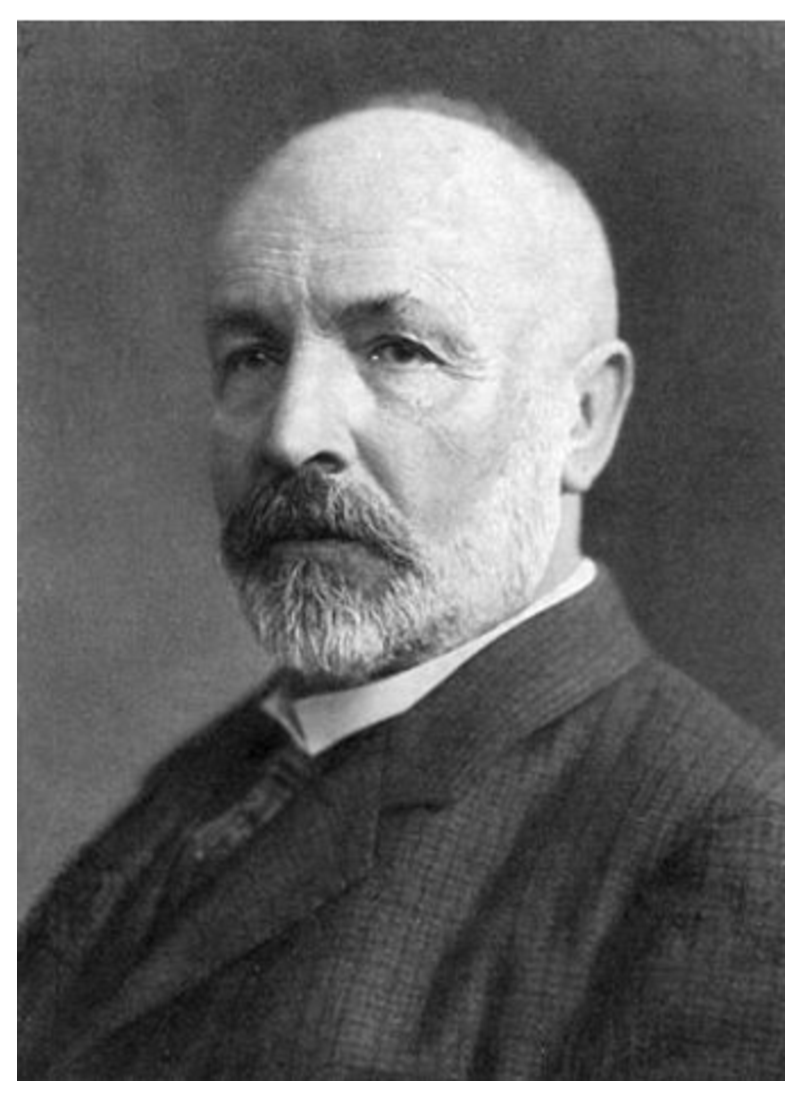
\includegraphics[width=2cm]{Georg-Cantor}}
\noindent\textbf{Georg Cantor} (1845--1918) was born in Saint Petersburg, Russia, where his father was a
successful merchant. Cantor, the oldest of six children, ever regarded as an outstanding violinist, developed his interest in mathematics in his teens. He began his university studies
in Zurich in 1862, but when his father died he left Zurich. He continued his university studies at the University
of Berlin in 1863, where he studied under the eminent mathematicians \underline{Karl Weierstrass} (1815--1897, German mathematician often cited as the ``father of modern analysis''), \underline{Ernst Eduard Kummer} (1810--1893, German mathematician), and \underline{Leopold Kronecker} (1823--1891, German mathematician whose doctrine is ``God made the integers, all else is the work of man.''). He received his doctor's degree in 1867, after having written a dissertation on number theory. Cantor assumed a position at the University of Halle (renamed Martin-Luther-Universit\"{a}t Halle-Wittenberg in 1933) in 1869, where he continued working until his death.
\\
He invented set theory, which has become a fundamental theory in mathematics.
Cantor's theory of \textit{transfinite numbers} was originally regarded as so counter-intuitive---even shocking---that it encountered resistance from mathematical contemporaries such as \underline{Leopold Kronecker} and \underline{Henri Poincar\'{e}} (1854--1912, French mathematician, theoretical physicist, engineer, and philosopher of science) and later from \underline{Hermann Weyl} (1885--1955, a German mathematician, theoretical physicist and philosopher) and \underline{L. E. J. Brouwer} (1881--1966, a Dutch mathematician and philosopher), while \underline{Ludwig Wittgenstein} (1889--1951, an Austrian-British philosopher) raised philosophical objections.
The objections to Cantor's work were occasionally fierce: \underline{Henri Poincar\'{e}} referred to his ideas as a ``grave disease'' infecting the discipline of mathematics, and Leopold Kronecker's public opposition and personal attacks included describing Cantor as a ``scientific charlatan'', a ``renegade'' and a ``corrupter of youth''.
\\
The harsh criticism has been matched by later accolades. In 1904, the Royal Society awarded Cantor its Sylvester Medal (James Joseph Sylvester (1814--1897), an English mathematician who made fundamental contributions to matrix theory, invariant theory, number theory, partition theory, and combinatorics), the highest honor it can confer for work in mathematics. \underline{David Hilbert} (1862--1943, German mathematician) defended Cantor's theory from its critics by declaring:\\
From his paradise that Cantor with us unfolded, we hold our breath in awe; knowing, we shall not be expelled.\\
Cantor married Vally Guttmann in 1874 and had five children. His melancholy temperament was balanced by his wife's happy disposition. Although he received a large inheritance from his father, he was poorly paid as a professor. To mitigate this, he tried to obtain a better-paying position at the University of Berlin but was blocked by Kronecker. Cantor suffered from mental illness (chronic depression or a bipolar disorder) from 1884 to the end of his life, which have been blamed on the hostile attitude of many of his contemporaries. Cantor retired in 1913, living in poverty and suffering from malnourishment during World War I (1914--1918). The public celebration of his 70th birthday was canceled because of the war. He died on January 6, 1918 from a heart attack in the sanatorium where he had spent the final year of his life. In Halle (Saale), where the Martin-Luther-Universit\"{a}t Halle-Wittenberg locates, there is a high school named Georg Cantor Gymnasium that is famous for teaching in mathematics and natural science.}


\textbf{Venn Diagrams}~~Sets can be represented graphically using Venn diagrams (also called primary diagrams, set diagrams or logic diagrams), named after the English mathematician
John Venn \footnote{\parpic{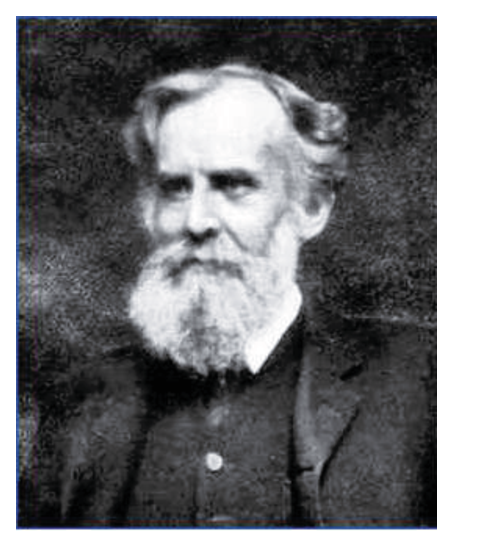
\includegraphics[width=2cm]{Venn}}
\noindent\textbf{John Venn} (1834--1923) was as an English logician and philosopher noted for introducing the Venn diagram, used in the fields of set theory, probability, logic, statistics, and computer science.
\\He began his education in London joining Sir Roger Cholmeley's School, now known as Highgate School, with his brother Henry in September 1846. In 1857, he obtained his degree in mathematics and became a fellow. In 1903 he was elected President of the College, a post he held until his death. In 1862, he returned to Cambridge as a lecturer in moral science, studying and teaching logic and probability theory, and, beginning around 1869, giving intercollegiate lectures. These duties led to his developing the diagram which would eventually bear his name.
\\
Venn built rare machines. The function of the machine was to bowl cricket balls. The machine was so fascinating that when the Australians were visiting Cambridge, the machines were used to entertain them. The bowl cricket ball that Venn built actually bowled out the top ranked player of the team four times consecutively.
\\
Venn was president of the Cambridge Antiquarian Society for 1908-1909. He is also listed as a vice president of the Cambridge Provident Medical Institution. Venn was a prominent supporter of votes for women. He co-signed with his wife Susanna, a letter to the Cambridge Independent Press published 16 October 1908, encouraging women to put themselves forward as candidates for the up-and-coming Cambridge town council elections. The letter was co-sponsored by Lady \underline{Maud Darwin}, wife of Sir \underline{George Darwin} (1845--1912, English barrister and astronomer, born at Down House, Kent, the second son and fifth child of Charles Darwin) and daughter-in-law of \underline{Charles Darwin} (1809--1882, English naturalist, geologist and biologist, best known for his contributions to the science of evolution), plus \underline{Florence Ada Keynes} (1861--1958, female, British author, historian and politician), who would later go on to become the first woman elected to Cambridge Town Council (now Cambridge City Council) and the second woman to become Mayor of Cambridge, in 1932-1933. She's also known for being the mother of the economist \underline{John Maynard Keynes} (1883--1946, British economist whose ideas fundamentally changed the theory and practice of macroeconomics and the economic policies of governments. He built on and greatly refined earlier work on the causes of business cycles, and is widely considered to be one of the most influential economists of the 20th century and the founder of modern macroeconomics theory. His ideas are the basis for the \textit{school of thought} known as \textit{Keynesian economics}, and its various offshoots.).}, who introduced their use in 1881. In Venn diagrams the universal set $U$, which
contains all the objects under consideration, is represented by a rectangle (Note that the universal
set varies depending on which objects are of interest). Inside this rectangle, circles or
other geometrical figures are used to represent sets. Sometimes points are used to represent the
particular elements of the set. Venn diagrams are often used to indicate the relationships between
sets.

\begin{example}
Draw a Venn diagram that represents $V$, the set of vowels in the English alphabet.
We draw a rectangle to indicate the universal set $U$, which is the set of the 26 letters
of the English alphabet. Inside this rectangle we draw a circle to represent $V$. Inside this circle
we indicate the elements of $V$ with points, as seen in Figure \ref{fig1-001}. \hfill$\square$
\end{example}





\begin{figure}[htbp]
%\sidecaption
%\includegraphics[scale=.45]{fig1-001.eps}
%\begin{center}
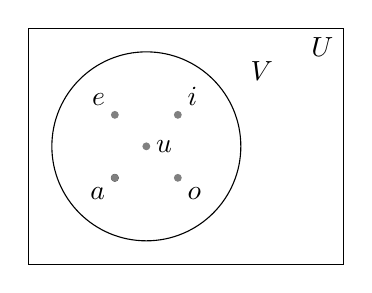
\begin{tikzpicture}
\fill[black] (-0.4,-0.4) circle (0.05cm);
\fill[gray] (-0.4,0.4) circle (0.05cm);
\fill[gray] (-0.4,-0.4) circle (0.05cm);
\fill[gray] (0.4,0.4) circle (0.05cm);
\fill[gray] (0.4,-0.4) circle (0.05cm);
\fill[gray] (0,0) circle (0.05cm);
\draw (0,0) circle (1.2cm);
\draw (-1.5,-1.5) rectangle (2.5,1.5) node [text=black,below left] {$U$};
\draw (-0.4,-0.4) node [text=black,below left] {$a$};
\draw (-0.4,0.4)  node [text=black,above left] {$e$};
\draw (0.4,0.4)   node [text=black,above right] {$i$};
\draw (0.4,-0.4)  node [text=black,below right] {$o$};
\draw (1.2,1.2)   node [text=black,below right] {$V$};
\draw (0,0)       node [text=black,right] {$u$};
\end{tikzpicture}
%\end{center}
\caption{Venn graph for the set of vowels.}
\label{fig1-001}       % Give a unique label
\end{figure}



It is common to encounter situations where the elements of one set are also the elements of
a second set. We now introduce some terminologies and notations to express such relationships
between sets.

\begin{definition}
The set $A$ is a subset of $B$ if and only if every element of $A$ is also an element of $B$. We use
the notation $A\subseteq{B}$ to indicate that $A$ is a subset of the set $B$.
\end{definition}


We see that $A\subseteq B$ if and only if the quantification

\[\forall x(x\in A\Rightarrow{x}\in{B})\]

\noindent is true. Note that to show that $A$ is not a subset of $B$ we need only find one element $x\in{A}$ with
$x\notin{B}$. Such an $x$ is a counterexample to the claim that $x\in{A}$ implies $x\in{B}$.


\begin{example}
The set of all odd positive integers less than 10 is a subset of the set of all positive integers less
than 10, the set of rational numbers is a subset of the set of real numbers, the set of all computer
science majors at your school is a subset of the set of all students at your school, and the set of
all people in China is a subset of the set of all people in China (that is, it is a subset of itself).
Each of these facts follows immediately by noting that an element that belongs to the first set
in each pair of sets also belongs to the second set in that pair.
\hfill$\square$
\end{example}



\begin{example}
The set of integers with squares less than 100 is not a subset of the set of nonnegative integers because -1 is in the former set (as $(-1)^2<100$), but not the later set. The set of people who
have taken discrete mathematics at your school is not a subset of the set of all computer science majors at your school if there is at least one student who has taken discrete mathematics who is
not a computer science major.
\hfill$\square$
\end{example}

Given any nonempty set $S$, it is guaranteed to have at least two subsets, the empty set and the set $S$ itself, that is, $\emptyset\subseteq{S}$ and $S\subseteq{S}$.

When we wish to emphasize that a set $A$ is a subset of a set $B$ but that $A\neq B$, we write
$A\subset{B}$ and say that $A$ is a \textit{proper subset} of $B$. For $A\subset{B}$ to be true, it must be the case that
$A\subseteq{B}$ and there must exist an element $x$ of $B$ that is not an element of $A$. That is, $A$ is a proper
subset of $B$ if and only if

\[\forall x(x\in{A}\Rightarrow x\in{B})\wedge\exists{y}(y\in{B}\wedge y\notin{A})\]


\noindent is true. Venn diagrams can be used to illustrate that a set $A$ is a subset of a set $B$. We draw the
universal set $U$ as a rectangle. Within this rectangle we draw a circle for $B$. Because $A$ is a subset
of $B$, we draw the circle for $A$ within the circle for $B$. This relationship is shown in Figure \ref{fig1-002}.



\begin{figure}[htbp]
%\sidecaption
%\includegraphics[scale=.45]{fig1-002.eps}
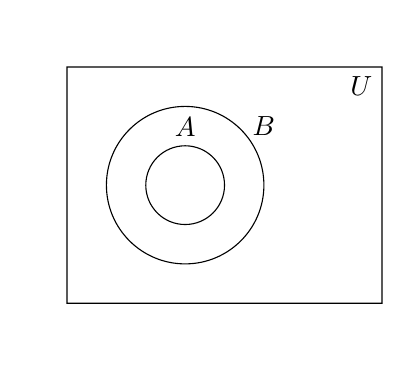
\begin{tikzpicture}[fill=gray]
% left hand
\scope
\clip (-2,-2) rectangle (2,2)
      (1,0) circle (1);
%\fill (0,0) circle (1);
\endscope
% right hand
\scope
\clip (-2,-2) rectangle (2,2)
      (0,0) circle (1);
%\fill (1,0) circle (1);
\endscope
% outline
%\fill[gray] (0,0) circle (0.5);
\draw (0,0) circle (0.5) (0,0.5)  node [text=black,above] {$A$}
      (0,0) circle (1) (1,1)  node [text=black,below] {$B$}
      (-1.5,-1.5) rectangle (2.5,1.5) node [text=black,below left] {$U$};
\end{tikzpicture}
\caption{Venn graph showing that $A$ is a proper subset of $B$.}
\label{fig1-002}       % Give a unique label
\end{figure}





A useful way to show that two sets have the same elements is to show that each set is a subset of the other. In other words, we can show that if $A$ and $B$ are sets with $A\subseteq{B}$ and $B\subseteq{A}$, then $A=B$. That is, $A=B$ if and only if $\forall x(x\in A\Rightarrow x\in{B})$ and $\forall x(x\in{B}\Rightarrow x\in A)$ or
equivalently if and only if $\forall x(x\in{A}\Leftrightarrow x\in{B})$, which is what it means for the $A$ and $B$ to be
equal.

\begin{example}
$A=\{\emptyset, \{a\}, \{b\}, \{a,b\}\}$ and $B=\{x|x~\text{is a subset of the set}~\{a,b\}\}$ are equal.
\hfill$\square$
\end{example}



\textbf{The Size of a Set}~~Sets are used extensively in counting problems, and for such applications we need to discuss
the sizes of sets.

\begin{definition}
Let $S$ be a set. If there are exactly $n$ distinct elements in $S$ where $n$ is a nonnegative integer,
we say that $S$ is a finite set and that $n$ is the cardinality of $S$. The cardinality of S is denoted by $|S|$.
\end{definition}


\begin{example}
Let $A$ be the set of odd positive integers less than 10. Then $|A|=5$. \hfill$\square$
\end{example}

\begin{example}
Let $S$ be the set of letters in the English alphabet. Then $|S|= 26$. \hfill$\square$
\end{example}



\begin{example}
Because the null set has no elements, it follows that $|\emptyset| =0$. \hfill$\square$
\end{example}

A set is said to be \textit{infinite} if it is not finite. For example, the set of all nonnegative integers $\{0, 1, 2, \ldots\}$ is infinite and the set of all even nonnegative numbers $\{0, 2, 4, \ldots\}$ is infinite. It is obvious that $\{0, 2, 4, \ldots\}$ is a proper subset of $\{0, 1, 2, \ldots\}$.
We will extend the notion of cardinality to infinite sets in Section 2.5, which is a challenging topic
full of surprising results \footnote{For a finite set, its cardinality provides an exact measure of its size. However, for infinite sets, the cardinality is a relative measure of two sets. Specifically, we can define what it means for one infinite set to have a small cardinality than another infinite set. The pertinent results regarding this issue are largely attributed to the work of Cantor and Julius Wilhelm Richard Dedekind (1831--1916). A primary surprising result is that sets $A=\{2, 4, 6, \ldots\}$ and $\mathbb{N}^+=\{1, 2, 3, \ldots\}$ have the same cardinality, represented by $|A|=|\mathbb{N}^+|$ (although $A\subset\mathbb{N}^+$ is obviously true). Since the concept of functions is needed to define the cardinality of an infinite set, we leave the problem in Chapter 2.}.


\textbf{Power Sets}~~Many problems involve testing all combinations of elements of a set to see if they satisfy some
property. To consider all such combinations of elements of a set $S$, we build a new set that has
as its members all the subsets of $S$.


\begin{definition}
Given a set $S$, the power set of $S$ is the set of all subsets of the set $S$. The power set of $S$ is
denoted by $\mathcal{P}(S)$.
\end{definition}



\begin{example}
The power set $\mathcal{P}(\{0, 1, 2\})$ is the set of all subsets of \{0, 1, 2\}. Hence,
$\mathcal{P}(\{0, 1, 2\})=\{\emptyset, \{0\}, \{1\}, \{2\}, \{0, 1\}, \{0, 2\}, \{1, 2\}, \{0, 1, 2\}\}$.
\hfill$\square$
\end{example}


\begin{example}
We have $\mathcal{P}(\emptyset)=\{\emptyset\}$ and $\mathcal{P}(\{\emptyset\})=\{\emptyset, \{\emptyset\}\}$.
\hfill$\square$
\end{example}

\begin{remark}
If a set $A$ has $n$ (disctinct) elements, then its power set contains $2^n$ members. Accordingly, sometimes $\mathcal{P}$ is written as $2^A$. \hfill$\square$
\footnote{\parpic{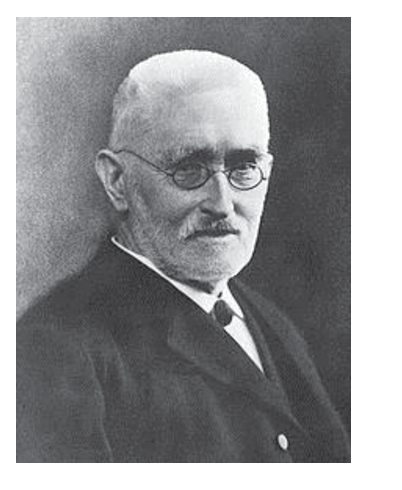
\includegraphics[width=2.0cm]{Dedekind.eps}}\noindent Julius Wilhelm Richard Dedekind (1831--1916) was a German mathematician who made important contributions to abstract algebra (particularly ring theory), algebraic number theory and the definition of the real numbers.\\
He was born, lived most of his life, and died in Braunschweig (often called ``Brunswick'' in English).
He first attended the Collegium Carolinum in 1848 before transferring to the University of G\"{o}ttingen in 1850. There, Dedekind was taught number theory by Professor Moritz Stern and he became Gauss's last student there. Dedekind received his doctorate in 1852. The thesis however did not display the talent evident by his subsequent work.\\
Dedekind went to Berlin for two years of study, where he and Bernhard Riemann (1826--1866, a German mathematician who made contributions to analysis, number theory, and differential geometry) were contemporaries; they were both awarded the habilitation in 1854. Dedekind returned to G\"{o}ttingen to teach, giving courses on probability and geometry. He studied for a while with Peter Gustav Lejeune Dirichlet (1805--1859, a German mathematician who made deep contributions to number theory, Fourier series and other topics in mathematical analysis, credited with being one of the first mathematicians to give the modern formal definition of a function), and they became good friends.
\\
Dedekind developed the notion now known as a Dedekind cut, now a standard definition of the real numbers.
In 1888, he published a short monograph titled ``What are numbers and what should they be?'' which included his definition of an infinite set. He also proposed an axiomatic foundation for the natural numbers, whose primitive notions were the number one and the successor function. In 1872, while on holiday in Interlaken, Dedekind met Georg Cantor. Thus they began an enduring relationship of mutual respect, and Dedekind became one of the very first mathematicians to admire Cantor's work concerning infinite sets, proving a valued ally in Cantor's disputes with Leopold Kronecker, who was philosophically opposed to Cantors's transfinite numbers.\\
He retired in 1894, but did occasional teaching and continued to publish. He never married, instead living with his sister Julia.
Dedekind was elected to the Academies of Berlin (1880) and Rome, and to the French Academy of Sciences (1900). He received honorary doctorates from the universities of Oslo, Zurich, and Braunschweig.\\
Interestingly and accidentally, Johann Carl Friedrich Gauss (1777--1855, a German mathematician who contributed significantly to many fields, including number theory, algebra, statistics, analysis, differential geometry, geodesy, geophysics, mechanics, electrostatics, astronomy, matrix theory, and optics, referred to as ``the foremost of mathematicians'' and ``greatest mathematician since antiquity''. Gauss had an exceptional influence in many fields of mathematics and science and is ranked as one of history's most influential mathematicians) was also born in the small town Braunschweig (252,768 people, as of 31 December 2015), where the residents are all proud of the two mathematicians.\\
There is an anecdote regarding the death of Dedekind. He lived so long that although some of his work had been familiar to all the students of analysis for a generation before his death, he himself had become almost a legend and many classed him with the shadowy dead. Twelve years before his death, a book \textit{Calendar for Mathematicians} listed Dedekind as having died on September 4, 1899, much to Dedekind's amusement. The day, September 4, might possible prove to be correct, he wrote to the editor of the book, but the year was certainly wrong.  `According to my memorandum I passed this day in perfect health and enjoyed a very stimulating conversation on ``system and theory'' with my luncheon guest and honoured friend Georg Cantor of Halle.'}
\end{remark}

\begin{remark}
For a finite non-empty set $A$, it is rather intuitive that the cardinality of set $A$ is strictly less than that of its power set $2^A$ or $\mathcal{P}(A)$, i.e., $|A|<|\mathcal{P}(A)|$. When $A$ is infinite, $\mathcal{P}(A)$ is naturally infinite. The relative measure of $|A|$ and $|\mathcal{P}(A)|$ is important for mathematics analysis. \hfill$\square$
\end{remark}


\textbf{Cartesian Products}~~The order of elements in a collection is often important. Because sets are unordered, a different
structure is needed to represent ordered collections. This is provided by \textbf{ordered $n$-tuples}.

\begin{definition}
An ordered $n$-tuple $(a_1, a_2, \ldots, a_n)$ is the ordered collection that has $a_1$ as its first element,
$a_2$ as its second element, $\ldots$, and $a_n$ as its $n$-th element.
\end{definition}

We say that two ordered $n$-tuples are equal if and only if each corresponding pair of their
elements is equal. In other words, $(a_1, a_2, \ldots, a_n)=(b_1, b_2, \ldots, b_n)$ if and only if $a_i=b_i$,
for $i=1, 2, \ldots, n$. In particular, ordered 2-tuples are called ordered pairs. The ordered pairs
$(a, b)$ and $(c, d)$ are equal if and only if $a=c$ and $b=d$. Note that $(a, b)$ and $(b, a)$ are not
equal unless $a=b$.

Many of the discrete structures are based on the notion of the
Cartesian product of sets (named after Ren\'{e} Descartes). We first define the Cartesian product
of two sets \footnote{\parpic{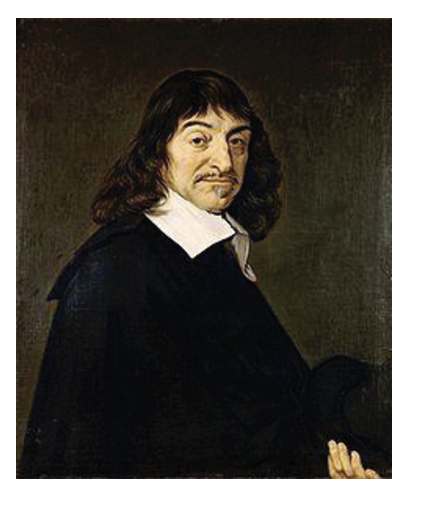
\includegraphics[width=2cm]{Descartes.eps}}\noindent Ren\'{e} Descartes (1596--1650) was a French philosopher, mathematician, and scientist. Dubbed the father of modern western philosophy, much of subsequent Western philosophy is a response to his writings, which are studied closely to this day.\\
Descartes was born into a noble family near Tours, France, about
200 miles southwest of Paris. He was the third child of his father's first wife. When he was one year old, his mother Jeanne Brochard died after trying to give birth to another child who also died. Because of Ren\'{e}'s poor health, his father, a provincial judge, let his son's formal lessons slide until, at
the age of 8, Ren\'{e} entered the Jesuit college at La Fl\`{e}che. The rector of the school took a liking to him and
permitted him to stay in bed until late in the morning because of his frail health. From then on, Descartes spent
his mornings in bed; he considered these times his most productive hours for thinking.\\
Descartes left school in 1612, moving to Paris, where he spent 2 years studying mathematics. He earned
a law degree in 1616 from the University of Poitiers. At 18 Descartes became disgusted with studying and
decided to see the world. He moved to Paris and became a successful gambler. However, he grew tired
of bawdy living and moved to the suburb of Saint-Germain, where he devoted himself to mathematical study. When his gambling
friends found him, he decided to leave France and undertake a military career. However, he never did any fighting. One day, while
escaping the cold in an overheated room at a military encampment, he had several feverish dreams, which revealed his future career as a mathematician and philosopher.\\
After ending his military career, he traveled throughout Europe. He then spent several years in Paris, where he studied mathematics and philosophy and constructed optical instruments. Descartes decided to move to Holland, where he spent 20 years wandering around the country, accomplishing his most important work. During this time he wrote several books, including the \textit{Discours}, which contains his contributions to analytic geometry, for which he is best known. He also made fundamental contributions to philosophy. \\
In 1649 Descartes was invited by Queen Christina to visit her court in Sweden to tutor her in philosophy. Although he was
reluctant to live in what he called ��the land of bears amongst rocks and ice,�� he finally accepted the invitation and moved to Sweden. Unfortunately, the winter of 1649--1650 was extremely bitter. Descartes caught pneumonia and died in mid-February.\\
One of Descartes' most enduring legacies was his development of Cartesian or analytic geometry, which uses algebra to describe geometry. He invented the convention of representing unknowns in equations by $x$, $y$, and $z$, and knowns by $a$, $b$, and $c$. He also pioneered the standard notation that uses superscripts to show the powers or exponents, e.g., $x^3$.
\\Current opinion is that Descartes had the most influence of anyone on the young Newton, and this is arguably one of Descartes' most important contributions. Newton continued Descartes' work on cubic equations, which freed the subject from the fetters of the Greek perspectives. Descartes' work provided the basis for the \textit{calculus} developed by Isaac Newton (1642--1726) and Gottfried Leibniz (1646--1716), who applied infinitesimal calculus to the tangent line problem, thus permitting the evolution of that branch of modern mathematics.}.



\begin{definition}
Let $A$ and $B$ be sets. The Cartesian product of $A$ and $B$, denoted by $A\times{B}$, is the set of all
ordered pairs $(a, b)$, where $a\in{A}$ and $b\in{B}$, i.e.,

\[A\times{B}=\{(a, b)|a\in A\wedge b\in B\}.\]
\end{definition}


\begin{example}
Let $A$ represent the set of all students at a university, and let $B$ represent the set of all courses
offered at the university. The Cartesian product $A\times{B}$ consists of all the ordered pairs of the form $(a, b)$, where
$a$ is a student at the university and $b$ is a course offered at the university. One way to use the set
$A\times{B}$ is to represent all possible enrollments of students in courses at the university.
\hfill$\square$
\end{example}


\begin{example}
Let $A=\{1, 2\}$ and $B=\{a, b, c\}$. The Cartesian product $A\times{B}$ is
$A\times{B}=\{(1, a), (1, b), (1, c), (2, a), (2, b), (2, c)\}$.
\hfill$\square$
\end{example}


If any of $A$ and $B$ is empty, $A\times{B}=B\times{A}=\emptyset$. However, in general, $A\times{B}\neq{B\times{A}}$ unless $A=B$. The Cartesian product of more than two sets can also be defined.

\begin{definition}
The Cartesian product of the sets $A_1$, $A_2$, $\ldots$, $A_n$, denoted by $A_1\times{A_2}\times\ldots\times{A_n}$, is the
set of ordered $n$-tuples $(a_1, a_2, \ldots, a_n)$, where $a_i$ belongs to $A_i$ for $i=1, 2, \ldots, n$. In other
words,

\[A_1\times A_2\times\ldots\times A_n=\{(a_1, a_2, \ldots, a_n)|a_i\in A_i~\text{for}~i=1,2, \ldots, n\}.\]
\end{definition}


\begin{example}
Let $A=\{0, 1\}, B=\{1, 2\}$, and $C=\{0, 1, 2\}$. $A\times{B}\times{C}$ consists of all ordered triples $(a, b, c)$, where $a\in{A}$, $b\in{B}$, and $c\in{C}$. Hence,

$A\times{B}\times{C}=\{(0, 1, 0), (0, 1, 1), (0, 1, 2), (0, 2, 0), (0, 2, 1), (0, 2, 2)$, $(1$, $1$, $0)$, $(1$, $1$, $1)$, $(1$, $1, 2), (1, 2, 0), (1, 2, 1), (1, 2, 2)\}.$
\hfill$\square$
\end{example}


We use the notation $A^2$ to denote $A\times{A}$, the Cartesian product of the set $A$ with itself.
Similarly, $A^3=A\times{A}\times{A}$, $A^4=A\times{A}\times{A}\times{A}\times{A}$, and so on. More generally,

\[A^n =\{(a_1, a_2, \ldots, a_n) | a_i\in A~\text{for}~i=1, 2, \ldots, n\}.\]


\begin{example}
Let $A=\{1, 2\}$ be a set. It follows that $A^2=\{(1, 1), (1, 2), (2, 1), (2, 2)\}$ and $A^3=\{(1, 1, 1), (1, 1, 2), (1, 2, 1), (1, 2, 2), (2, 1, 1), (2, 1, 2), (2, 2, 1), (2, 2, 2)\}$.
\hfill$\square$
\end{example}


A subset $R$ of the Cartesian product $A\times{B}$ is called a relation \footnote{\textit{Relation} is an important concept in discrete mathematics, which will be introduced in Chapter 3.} from the set $A$ to the set
$B$. The elements of $R$ are ordered pairs, where the first element belongs to $A$ and the second
to $B$. For example, $R=\{(a, 0), (a, 1), (a, 3), (b, 1), (b, 2), (c, 0), (c, 3)\}$ is a relation from the
set $\{a, b, c\}$ to the set $\{0, 1, 2, 3\}$. A relation from a set $A$ to itself is called a relation on $A$.


Suppose that $A$=\{G88\} and $B$=\{Xian, Zhengzhou, Hebi, Xingtai, Shijiazhuang, Baoding, Beijing\}. Then $R$=\{(G88, Xian), (G88, Zhengzhou), (G88, Shijiazhuang), (G88, Beijing)\} is a relation from $A$ to $B$, indicating the cites in which High Speed Rail G88 (China Railway Corporation) stops over.

\begin{example}
Let $A=\{0,1,2,3\}$ and $R=\{(a,b)|a\leq{b}\}$ be a relation on $A$. Then
$R=\{(0,0)$, $(0,1), (0,2), (0,3), (1,1), (1,2), (1,3),
(2,2), (2, 3), (3, 3)\}$. \hfill$\square$
\end{example}

\section{Set Operations}

Two, or more, sets can be combined in many different ways. For instance, starting with the set
of mathematics majors at your school and the set of computer science majors at your school, we
can form the set of students who are mathematics majors or computer science majors, the set of
students who are joint majors in mathematics and computer science, the set of all students not
majoring in mathematics, and so on.

\begin{definition}
Let $A$ and $B$ be sets. The union of the sets $A$ and $B$, denoted by $A\cup{B}$, is the set that contains
those elements that are either in $A$ or in $B$, or in both.
\end{definition}

An element $x$ belongs to the union of the sets $A$ and $B$ if and only if $x$ belongs to $A$ or $x$ belongs
to $B$. This tells us that

\[A\cup B=\{x|x\in{A}\vee x\in{B}\}.\]


The Venn diagram shown in Figure \ref{union of two sets} represents the union of two sets $A$ and $B$. The area
that represents $A\cup{B}$ is the shaded area within either the circle representing $A$ or the circle
representing $B$.

\begin{figure}[htbp]
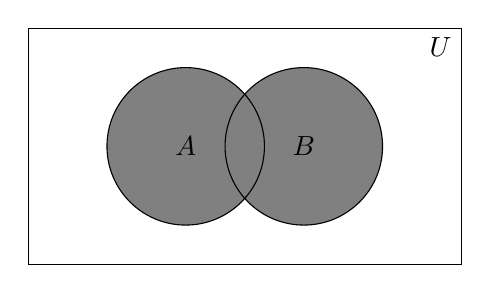
\begin{tikzpicture}
\draw (-2,-1.5) rectangle (3.5,1.5) node[below left]{$U$};
\fill[gray] (0,0) circle (1cm);
\fill[gray] (1.5,0) circle (1cm);
\draw (0,0) circle (1cm) node {$A$};
\draw (1.5,0) circle (1cm) node {$B$};
\end{tikzpicture}
\caption{Venn graph of the union of two sets.}
\label{union of two sets}
\end{figure}

\begin{example}
The union of the sets \{1, 3, 5\} and \{1, 2, 3\} is the set \{1, 2, 3, 5\}; that is,
\{1, 3, 5\}$\cup$\{1, 2, 3\}=\{1, 2, 3, 5\}.
\hfill$\square$
\end{example}


\begin{example}
The union of the sets $\{a, b, c, d\}$ and $\{1, 2, b, d, e\}$ is the set $\{1$, $2$, $a$, $b$, $c$, $d$, $e\}$.
\hfill$\square$
\end{example}

\begin{example}
The union of the set of all computer science majors at Xidian University and the set of all mathematics
majors at Xidian University is the set of students at Xidian University who are majoring either in
mathematics or in computer science (or in both).
\hfill$\square$
\end{example}


\begin{definition}
Let $A$ and $B$ be sets. The \textit{intersection} of the sets $A$ and $B$, denoted by $A\cap{B}$, is the set
containing those elements in both $A$ and $B$.
\end{definition}

An element $x$ belongs to the intersection of the sets $A$ and $B$ if and only if $x$ belongs to $A$ and
$x$ belongs to $B$. This tells us that

\[A\cap{B}=\{x|x\in A\wedge x\in B\}.\]



The Venn diagram shown in Figure \ref{intersection of two sets} represents the intersection of two sets $A$ and $B$. The shaded
area that is within both the circles representing the sets $A$ and $B$ is the area that represents the
intersection of $A$ and $B$.

\begin{figure}[htbp]
%\begin{center}
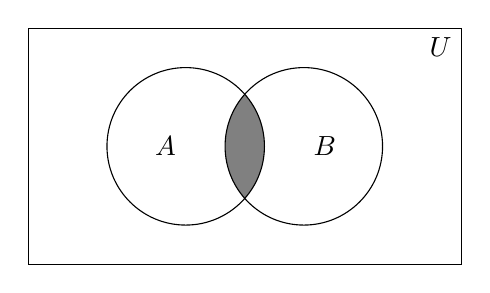
\begin{tikzpicture}
\draw (-2,-1.5) rectangle (3.5,1.5) node[below left]{$U$};
\begin{scope} % start of clip scope
\clip (0,0) circle (1cm);
\fill[gray] (1.5,0) circle (1cm);
\end{scope} % end of clip scope
\draw (0,0) circle (1cm) node[left] {$A$};
\draw (1.5,0) circle (1cm) node[right] {$B$};
\end{tikzpicture}
%\end{center}
\caption{Venn graph of the intersection of two sets.}
\label{intersection of two sets}
\end{figure}


\begin{example}
The intersection of the sets \{1, 3, 5\} and \{1, 2, 3\} is the set \{1, 3\}; that is,
$\{1, 3, 5\}\cap\{1, 2, 3\} = \{1, 3\}$.
\hfill$\square$
\end{example}


\begin{example}
The intersection of the set of all computer science majors at your school and the set of all
mathematics majors is the set of all students who are joint majors in mathematics and computer
science.
\hfill$\square$
\end{example}



We are often interested in finding the cardinality of a union of two finite sets $A$ and $B$. Note that $|A|+|B|$ counts each element that is in $A$ but not in $B$ or in $B$ but not in $A$ exactly once, and each element that is in both $A$ and $B$ exactly twice. Thus, if the number of elements that
are in both $A$ and $B$ is subtracted from $|A|+|B|$, elements in $A\cap B$ will be counted only once. Hence,

\[|A\cup B|=|A|+|B|-|A\cap B|.\]


\begin{definition}
Two sets are said to be \textit{disjoint} if their intersection is the empty set.
\hfill$\square$
\end{definition}


\begin{example}
Let $A=\{1, 3, 5, 7, 9\}$ and $B=\{2, 4, 6, 8, 10\}$. Because $A\cap B=\emptyset$, $A$ and $B$ are disjoint.
\hfill$\square$
\end{example}


\begin{definition}
Let $A$ and $B$ be sets. The \textit{difference} of $A$ and $B$, denoted by $A-B$ or $A\setminus{B}$, is the set containing those
elements that are in $A$ but not in $B$. The difference of $A$ and $B$ is also called the \textit{complement} of $B$ with respect to $A$.
\end{definition}

An element $x$ belongs to the difference of $A$ and $B$ if and only if $x\in A$ and $x\notin{B}$. This tells us
that

\[A-B=\{x|x\in A\wedge x\notin B\}.\]


The Venn diagram shown in Figure \ref{Difference of two sets} represents the difference of the sets $A$ and $B$. The shaded
area inside the circle that represents $A$ and outside the circle that represents $B$ is the area that
represents $A-B$.


\begin{figure}[htbp]
%\begin{center}
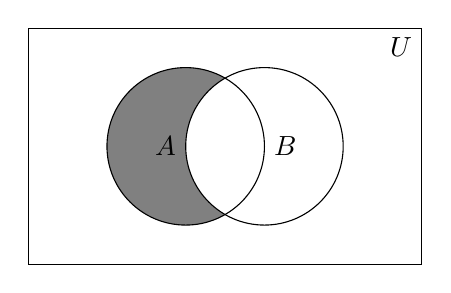
\begin{tikzpicture}
\draw (-2,-1.5) rectangle (3,1.5) node[below left]{$U$}; % draw a rectangle
\fill[gray] (0,0) circle (1cm); % then fill in a circular region
\fill[white] (1,0) circle (1cm); % then fill in a 2nd circular region
\draw (0,0) circle (1cm) node[left] {$A$};
\draw (1,0) circle (1cm) node[right] {$B$};
\end{tikzpicture}
%\end{center}
\caption{Venn graph of the difference of two sets.}
\label{Difference of two sets}
\end{figure}


\begin{example}
The difference of \{1, 3, 5\} and \{1, 2, 3\} is the set \{5\}; that is, $\{1, 3, 5\}-\{1, 2, 3\}=\{5\}$. This
is different from the difference of \{1, 2, 3\} and \{1, 3, 5\}, which is the set \{2\}.
\hfill$\square$
\end{example}

\begin{example}
The difference of the set of computer science majors at your school and the set of mathematics majors at your school is the set of all computer science majors at your school who are not also
mathematics majors.
\hfill$\square$
\end{example}



Once the universal set $U$ has been specified, the complement of a set can be defined.


\begin{definition}
Let $U$ be the universal set. The \textit{complement} of the set $A$, denoted by $\overline{A}$, is the complement
of $A$ with respect to $U$. Therefore, the complement of the set A is $U-A$.
\end{definition}

An element belongs to $\overline{A}$ if and only if $x\notin{A}$. This tells us that

\[\overline{A}=\{x\in U|x\notin A\}.\]


In Figure \ref{complement of a set} the shaded area outside the circle representing $A$ is the area representing $\overline{A}$.

\begin{figure}[htbp]
\begin{center}
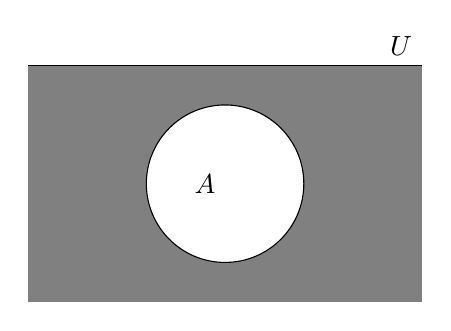
\begin{tikzpicture}
\draw (-2,-1.5) rectangle (3,1.5) node[above left] {$U$}; % draw a rectangle
\fill[gray] (-2,-1.5) rectangle (3,1.5); % then fill in a circular region
\fill[white] (0.5,0) circle (1cm); % then fill in a 2nd circular region
\draw (0.5,0) circle (1cm) node[left] {$A$};
\end{tikzpicture}
\caption{Venn diagram of the complement of a set.}
\label{complement of a set}
\end{center}
\end{figure}

\begin{example}
Let $A=\{a, e, i, o, u\}$ (where the universal set is the set of letters of the English alphabet). Then
$\overline{A}=\{b, c, d, f, g, h, j, k, l, m, n, p, q, r, s, t, v, w, x, y, z\}$.
\hfill$\square$
\end{example}


\begin{example}
Let $A$ be the set of positive integers greater than 10 (with universal set the set of all positive
integers). Then $\overline{A}=\{1, 2, 3, 4, 5, 6, 7, 8, 9, 10\}$.
\hfill$\square$
\end{example}


\textbf{Set Identities}~~
Table \ref{set identities} lists the most important set identities. We can prove these identities
using different methods. These methods are presented to illustrate that there are often many
different approaches to the solution of a problem. The proofs of the remaining identities will
\marginpar{\small Set identities and propositional equivalences are just special cases of identities
for Boolean algebra.}
be left as exercises. The reader should note the similarity between these set identities and the
logical equivalences. In fact, the set identities given can be proved directly from the corresponding logical equivalences.
Furthermore, both are special cases of identities that hold for Boolean algebra.

\begin{table}
\caption{Set identities}
\begin{tabular}{|p{8cm}||p{3cm}|}
  \hline
  Identity & Name\\
  \hline
  $A\cap{U}=A$, $A\cup\emptyset=A$ & Identity laws \\
  \hline
  $A\cup{U}=U$, $A\cap\emptyset=\emptyset$ & Domination laws \\
  \hline
  $A\cup{A}=A$, $A\cap{A}=A$ & Idempotent laws \\
  \hline
  $\overline{(\overline{A})}=A$ & Complementation law \\
  \hline
  $A\cup{B}=B\cup{A}$, $A\cap{B}=B\cap{A}$ & Commutative laws \\
  \hline
  $A\cup{(B\cup C)}=(A\cup B)\cup{C}$, $A\cap{(B\cap C)}=(A\cap{B})\cap{C}$ & Associative laws \\
  \hline
  $A\cup(B\cap C)=(A\cup B)\cap(A\cup C)$, $A\cap (B\cup C)=(A\cap B)\cup(A\cap C)$ & Distributive laws \\
  \hline
  $\overline{A\cap B}=\overline{A}\cup\overline{B}$, $\overline{A\cup{B}}=\overline{A}\cap\overline{B}$ & De Morgan's laws\\
    \hline
  $A\cup(A\cap B)=A$, $A\cap(A\cup B)=A$ & Absorption laws \\
  \hline
  $A\cup\overline{A}=U$, $A\cap\overline{A}=\emptyset$ & Complement laws \\
  \hline
\end{tabular}
\label{set identities}
\end{table}

One way to show that two sets are equal is to show that each is a subset of the other. Recall
that to show that one set is a subset of a second set, we can show that if an element belongs to
the first set, then it must also belong to the second set. We generally use a direct proof to do this.
We illustrate this type of proof by establishing the first of De Morgan's laws.



\begin{example}
Prove that $\overline{(A\cap B)}=\overline{A}\cup\overline{B}$.

Solution: First, we will show that $\overline{A\cap B}\subseteq\overline{A}\cup\overline{B}$. We do this by showing that if $x$ is in $\overline{A\cap B}$, then it must also be in $\overline{A}\cup\overline{B}$. Now suppose that $x\in\overline{A\cap B}$. By the definition of complement, $x\notin A\cap B$. Using the definition of intersection, we see that the proposition $\neg((x\in A) \wedge(x\in B))$ is true.

By applying De Morgan's law for propositions, we see that $\neg(x\in A)$ or $\neg(x\in B)$. Using
the definition of negation of propositions, we have $x\notin A$ or $x\notin B$. Using the definition of
the complement of a set, we see that this implies that $x\in\overline{A}$ or $x\in\overline{B}$. Consequently, by the
definition of union, we see that $x\in\overline{A}\cup\overline{B}$. We have now shown that $\overline{A\cap B}\subseteq\overline{A}\cup\overline{B}$.

Next, we will show that $\overline{A}\cup\overline{B}\subseteq\overline{A\cap B}$. We do this by showing that if $x$ is in $\overline{A}\cup\overline{B}$, then it must also be in $\overline{A\cap B}$. Now suppose that $x\in\overline{A}\cup\overline{B}$. By the definition of union, we know that
$x\in\overline{A}$ or $x\in\overline{B}$. Using the definition of complement, we see that $x\notin A$ or $x\notin B$. Consequently, the proposition $\neg(x\in A)\vee\neg(x\in B)$ is true.

By De Morgan's law for propositions, we conclude that $\neg((x\in A)\wedge(x\in B))$ is true.
By the definition of intersection, it follows that $\neg(x\in A\cap B)$. We now use the definition of
complement to conclude that $x\in\overline{A\cap B}$. This shows that $\overline{A}\cup\overline{B}\subseteq\overline{A\cap B}$.

Because we have shown that each set is a subset of the other, the two sets are equal, and the identity is proved. \marginpar{\small Mathematical induction, a form of direct proof, is a mathematical proof technique used to prove a given statement about any well-ordered set.} \footnote{\parpic{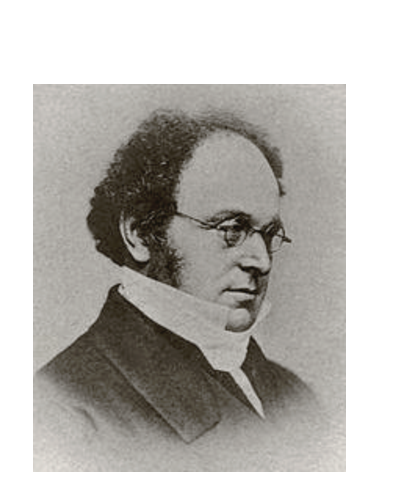
\includegraphics[width=2.0cm]{Morgan.eps}}Augustus De Morgan (1806--1871) was a British mathematician and logician. He formulated De Morgan's laws and introduced the term mathematical induction, making its idea rigorous. In his own time he was better known as a newspaper columnist.\\
De Morgan studied at Trinity College, Cambridge, graduating in 1827. Although he considered medicine or law, he decided on
mathematics for his career. In the 1840s De Morgan made fundamental contributions to the development of symbolic logic. He invented notations that helped him prove propositional equivalences, such as the laws that are named after him. In 1842 De Morgan presented what is considered to be the first precise definition of a limit and developed new tests for convergence of infinite series. De Morgan was also interested in the history of mathematics and wrote biographies of \underline{Newton} and \underline{Halley} (1656--1742, an English astronomer, geophysicist, mathematician, meteorologist, and physicist who is best known for computing the orbit of Halley's Comet).
\\
De Morgan was famous for his opposition to negative numbers, which nowadays flabbergasts our contemporaries since, without thinking too much about it, most of us can use negative numbers for things like recording temperatures below zero and representing economy recession by negative increase. It takes a long time until the end of the 19th century that negative numbers are well accepted by the community of mathematics as part of the number system. \\
Although the first set of rules for dealing with negative numbers was stated in the 7th century by the Indian mathematician Brahmagupta, it is surprising that in 1758 the British mathematician \underline{Francis Maseres} (1731--1824, an English lawyer, known as attorney general of the Province of Quebec, judge, mathematician, historian, and member of the Royal Society) was claiming that negative numbers\\
``\ldots\ldots darken the very whole doctrines of the equations and make dark of the things which are in their nature excessively obvious and simple''.\\
In the early work solving equations, negative roots were not even considered. Hindu mathematicians in the sixth century, and before that, Chinese mathematicians figured out all the rules for operations with negative numbers. Yet the Arabs did not include any of this in their work three centuries later. French mathematician \underline{Blaise Pascal} (1623-1662, a French mathematician, physicist, inventor, writer and Catholic theologian) did not see the need for negative numbers. De Morgan thought numbers less than zero were unimaginable. \\For females, De Morgan cautioned them against
studying too much mathematics, because it might interfere with their childbearing abilities.}
\hfill$\square$
\label{set identity 1}
\end{example}


We can more succinctly express the reasoning used in Example \ref{set identity 1} using set builder notation,
as Example \ref{set identity 2} illustrates

\begin{example}
Use set builder notation and logical equivalences to establish the first De Morgan law $\overline{A\cap B}=
\overline{A}\cup\overline{B}$.

Solution: We can prove this identity with the following steps.

$\overline{A\cap{B}}=\{x|x\notin A\cap{B}\}$ \hfill by definition of complement

$=\{x|\neg(x\in(A\cap B))\}$ \hfill by definition of ``does not belong symbol''

$=\{x|\neg(x\in A\wedge x\in B)\}$ \hfill by definition of intersection

$=\{x |\neg(x\in A)\vee\neg(x\in B)\}$ \hfill by the second De Morgan law

\hfill for logical equivalences
\marginpar{De Morgan's law for logical equivalence is $\neg(p\wedge q)=\neg p\vee\neg q$ and $\neg(p\vee q)=\neg p\wedge\neg q$, where $p$ and $q$ are propositions.}


$=\{x|x\notin A\vee\notin B\}$ \hfill by definition of ``does not belong symbol''

$=\{x|x\in\overline{A}\vee x\in\overline B\}$ \hfill by definition of complement

$=\{x|x\in\overline{A}\cup\overline{B}\}$ \hfill by definition of union

$=\overline{A}\cup\overline{B}$ \hfill by meaning of set builder notation

Note that besides the definitions of complement, union, set membership, and set builder
notation, this proof uses the second De Morgan law for logical equivalences.
\hfill$\square$
\label{set identity 2}
\end{example}


\begin{example}
Prove the second distributive law from Table 1, which states that
$A\cap (B\cup C)=(A\cap B)\cup (A\cap C)$ for all sets $A$, $B$, and $C$.


Solution: We will prove this identity by showing that each side is a subset of the other side.
Suppose that $x\in A\cap(B\cup C)$. Then $x\in A$ and $x\in B\cup C$. By the definition of union, it
follows that $x\in A$, and $x\in B$ or $x\in C$ (or both). In other words, we know that the compound
proposition $(x\in A)wedge((x\in B)\vee(x\in C))$ is true. By the distributive law for conjunction over
disjunction, it follows that $((x\in A)\wedge(x\in B))\vee((x\in A)\wedge(x\in C))$. We conclude that either
$x\in A$ and $x\in B$, or $x\in A$ and $x\in C$. By the definition of intersection, it follows that $x\in A\cap B$
or $x\in A\cap C$. Using the definition of union, we conclude that $x\in (A\cap B)\cup(A\cap C)$. We
conclude that $A\cap(B\cup C)\subseteq(A\cap B)\cup(A\cap C)$.


Now suppose that $x\in(A\cap B)\cup(A\cap C)$. Then, by the definition of union, $x\in A\cap B$ or
$x\in A\cap C$. By the definition of intersection, it follows that $x\in A$ and $x\in B$ or that $x\in A$ and
$x\in C$. From this we see that $x\in A$, and $x\in B$ or $x\in C$. Consequently, by the definition of
union we see that $x\in A$ and $x\in B\cup C$. Furthermore, by the definition of intersection, it follows
that $x\in A\cap (B\cup C)$. We conclude that $(A\cap B)\cup(A\cap C)\subseteq A\cap(B\cup C)$. This completes
the proof of the identity.
\hfill$\square$
\end{example}


Because unions and intersections of sets satisfy associative laws, the sets $A\cup B\cup C$ and
$A\cap B\cap C$ are well defined; that is, the meaning of this notation is unambiguous when $A$,
$B$, and $C$ are sets. That is, we do not have to use parentheses to indicate which operation
comes first because $A\cup(B\cup C)=(A\cup B)\cup C$ and $A\cap(B\cap C)=(A\cap B)\cap C$. Note that
$A\cup B\cup C$ contains those elements that are in at least one of the sets $A$, $B$, and $C$, and that
$A\cap B\cap C$ contains those elements that are in all of $A$, $B$, and $C$.


\begin{example}
Let $A=\{0, 2, 4, 6, 8\}$, $B=\{0, 1, 2, 3, 4\}$, and $C=\{0, 3, 6, 9\}$. The set $A\cup B\cup C$ contains those elements in at least one of $A$, $B$, and $C$. Hence, $A\cup B\cup C=\{0, 1, 2, 3, 4, 6, 8, 9\}$.
The set $A\cap B\cap C$ contains those elements in all three of $A$, $B$, and $C$. Thus, $A\cap B\cap C=\{0\}$.
\hfill$\square$
\end{example}




\begin{definition}
The union of a collection of sets is the set that contains those elements that are members of
at least one set in the collection.
\end{definition}

We use the notation

\[A_1\cup A_2\cup\ldots\cup A_n=\cup_{i=1}^{n}A_i\]

\noindent to denote the union of the sets $A_1$, $A_2$, $\ldots$, $A_n$.

\begin{definition}
The intersection of a collection of sets is the set that contains those elements that are members
of all the sets in the collection.
\end{definition}

We use the notation

\[A_1\cap A_2\cap\ldots\cap A_n=\cap_{i=1}^{n}A_i\]

\noindent to denote the intersection of the sets $A_1$, $A_2$, $\ldots$, $A_n$.


\begin{example}
For $i=1, 2, \ldots$, let $A_i=\{i, i + 1, i + 2, \ldots\}$. Then,


\[\cup_{i=1}^{n}A_i=\cup_{i=1}^{n}\{i, i+1, i+2, \ldots\}=\{1, 2, 3, \ldots\},\]

and

\[\cap_{i=1}^{n}A_i=\cap_{i=1}^{n}\{i, i+1, i+2, \ldots\}=\{n, n+1, n+2, \ldots\}=A_n.\]
\hfill$\square$
\end{example}


\begin{definition}
Let $A_1$, $A_2$, $\ldots$, $A_n$ be subsets of $S$. $A_1$, $A_2$, $\ldots$, $A_n$ are said to be a partition of $S$ if (1) $\cup_{i=1}^{n}A_i=S$ and (2) $\forall i\neq{j}$ $(i,j\in\mathbb{N}_n)$, $A_i\cap{A_j}=\emptyset$.
\end{definition}



\begin{example}
Consider the following collections of subsets of $S=\{1, 2, . . ., 8, 9\}$:

(i) \{1, 3, 5\}, \{2, 6\}, \{4, 8, 9\};

(ii) \{1, 3, 5\}, \{2, 4, 6, 8\}, \{5, 7, 9\}; and

(iii) \{1, 3, 5\}, \{2, 4, 6, 8\}, \{7, 9\}.

It is trivial that (i) and (ii) are not the partition of $S$, while (iii) is.
\hfill$\square$
\end{example}

\section{Multi-sets}

In mathematics, a \textit{multiset} (or \textit{bag}) is a generalization of the concept of a set that, unlike a set, allows multiple instances of the multiset's elements. For example, $\{a, a, b\}$ and $\{a, b\}$ are different multisets although they are the same set. However, the order in a multiset does not matter. Specifically, $\{a, a, b\}$ and $\{a, b, a\}$ are the same multiset.


\underline{De~Bruijn}\footnote{\parpic{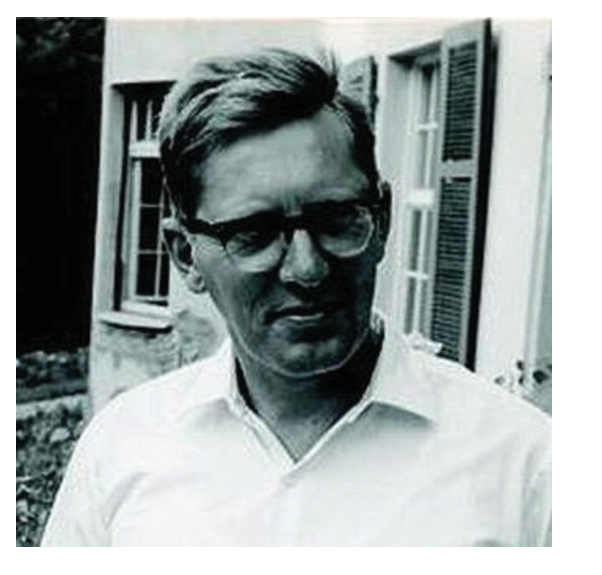
\includegraphics[width=2.0cm]{Bruijn.eps}}\noindent Nicolaas Govert de Bruijn (1918--2012) was a Dutch mathematician, noted for his many contributions in the fields of analysis, number theory, combinatorics and logic. De Bruijn started his academic career as at the University of Amsterdam, where he was Professor of Mathematics from 1952 to 1960. In 1960 he moved to the Technical University Eindhoven where he was Professor of Mathematics until his retirement in 1984.
In 1957 he was appointed member of the Royal Netherlands Academy of Arts and Sciences. He was Knighted with the Order of the Netherlands Lion.} coined the word \textit{multiset} in the 1970s. However, the use of multisets predates the word multiset by many centuries. The first study of multisets is usually attributed to an Indian mathematician who described permutations of multisets around 1150. In history, other names that were proposed or used for multisets include \textit{list}, \textit{bunch}, \textit{bag}, \textit{heap}, \textit{sample}, \textit{weighted set}, \textit{collection}, and \textit{suite}. The word ``visa'' is also used.

In the explicit form, multisets appeared in the work of \underline{Richard Dedekind}. Other mathematicians formalized multisets and began to study them as a precise mathematical object (structure) in the 20th century.

The multiplicity of an element is the number of instances of the element in a specific multiset. For example, an infinite number of multisets exist which contain only elements $a$ and $b$, varying only by multiplicity: The unique set $\{a, b\}$ contains only elements $a$ and $b$, each having multiplicity 1. In multiset $\{a, a, b\}$, $a$ has multiplicity 2 and $b$ has multiplicity 1.
In multiset $\{a, a, a, b, b, b\}$, $a$ and $b$ both have multiplicity 3.

\begin{definition}
Let $A$ be an ordinary set. A multiset $\alpha$ is a mapping from $A$ to $\mathbb{N}$ that gives the multiplicity of an element $a\in{A}$, denoted by $\alpha(a)$, representing the number of appearances of an element $a$ in $\alpha$. The cardinality of $\alpha$ is defined as $\sum_{a\in{A}}\alpha(a)$.
\end{definition}

By the definition, a multiset $\alpha$, given the underlying set $A$, can be written as $\alpha=\sum_{a\in{A}}\alpha(a).a$.

\begin{example}
In a multiset $\alpha=\{a, a, b, c, c, c\}$ on set $A=\{a, b, c, d\}$. We have $\alpha(a)=2$, $\alpha(b)=1$, $\alpha(c)=3$, and $\alpha(d)=0$. Then, the cardinality of $\alpha$, denoted as $|\alpha|$, is $\alpha(a)+\alpha(b)+\alpha(c)=6$. Write $\alpha=2a+b+3c$. For $x\in{A}$, If $\alpha(x)>0$, write $x\in\alpha$.
\end{example}

\begin{definition}
Let $\alpha$ and $\alpha^\prime$ be two multisets over a set $A$. Their addition, scalar multiplication, cover and substraction are defined as follows:

\begin{itemize}
  \item Addition: $\alpha+\alpha^\prime=_{\text{def}}\sum_{a\in{A}}(\alpha(a)+\alpha^\prime(a)).a$.
  \item Scalar multiplication: $n\times\alpha=_{\text{def}}\sum_{a\in{A}}(n\times\alpha(a)).a, n\in\mathbb{N}$.
  \item $\alpha$ covers $\alpha^\prime$: $\alpha\geq\alpha^\prime=_{\text{def}}\alpha(a)\geq\alpha^\prime(a), \forall a\in{A}$.
  \item $\alpha$ properly covers $\alpha^\prime$: $\alpha>\alpha^\prime=_{\text{def}}\alpha\geq\alpha^\prime$ and $\exists a\in{A}$, $\alpha(a)>\alpha^\prime(a)$.
  \item Substraction: $\alpha-\alpha^\prime=_{\text{def}}\sum_{a\in{A}}(\alpha(a)-\alpha^\prime(a)).a$ if $\alpha\geq\alpha^\prime$.
\end{itemize}
\end{definition}


\begin{definition}
A multiset $\alpha^\prime$ is said to be a subset of the multiset $\alpha$ if $\alpha\geq\alpha^\prime$. The power set of a multiset $\alpha$ (denoted as $2^\alpha$) is the set of all subsets of $\alpha$. If $\forall a\in{A}$, $\alpha(a)=0$, $\alpha$ is said to be an empty multiset. An empty multiset is usually written as $\emptyset$. We stipulate that $\emptyset\in 2^\alpha$ for any multiset $\alpha$.
\end{definition}

\begin{example}
Let $\alpha_1=2a+3b+c$ and $\alpha_2=a+2b$ be two multisets defined on a set $A=\{a, b, c, d\}$. We have $\alpha_1+\alpha_2=3a+5b+c$, $3\alpha_1=6a+9b+3c$, $\alpha_1\geq\alpha_2$, and $\alpha_1-\alpha_2=a+b+c$. Note that $2^{\alpha_2}=\{\emptyset, a, b, 2b, a+b, a+2b\}$. \hfill$\square$
\end{example}



\newpage
\section{Section Heading}
\label{sec:1}
Use the template \emph{chapter.tex} together with the Springer document class SVMono (monograph-type books) or SVMult (edited books) to style the various elements of your chapter content in the Springer layout.

\section{Section Heading}
\label{sec:2}
% Always give a unique label
% and use \ref{<label>} for cross-references
% and \cite{<label>} for bibliographic references
% use \sectionmark{}
% to alter or adjust the section heading in the running head
Instead of simply listing headings of different levels we recommend to let every heading be followed by at least a short passage of text. Furtheron please use the \LaTeX\ automatism for all your cross-references and citations.

Please note that the first line of text that follows a heading is not indented, whereas the first lines of all subsequent paragraphs are.

Use the standard \verb|equation| environment to typeset your equations, e.g.
%
\begin{equation}
a \times b = c\;,
\end{equation}
%
however, for multiline equations we recommend to use the \verb|eqnarray|
environment\footnote{In physics texts please activate the class option \texttt{vecphys} to depict your vectors in \textbf{\itshape boldface-italic} type - as is customary for a wide range of physical subjects.}.
\begin{eqnarray}
a \times b = c \nonumber\\
\vec{a} \cdot \vec{b}=\vec{c}
\label{eq:01}
\end{eqnarray}

\subsection{Subsection Heading}
\label{subsec:2}
Instead of simply listing headings of different levels we recommend to let every heading be followed by at least a short passage of text. Furtheron please use the \LaTeX\ automatism for all your cross-references\index{cross-references} and citations\index{citations} as has already been described in Sect.~\ref{sec:2}.

\begin{quotation}
Please do not use quotation marks when quoting texts! Simply use the \verb|quotation| environment -- it will automatically render Springer's preferred layout.
\end{quotation}


\subsubsection{Subsubsection Heading}
Instead of simply listing headings of different levels we recommend to let every heading be followed by at least a short passage of text. Furtheron please use the \LaTeX\ automatism for all your cross-references and citations as has already been described in Sect.~\ref{subsec:2}, see also Fig.~\ref{fig:1}\footnote{If you copy text passages, figures, or tables from other works, you must obtain \textit{permission} from the copyright holder (usually the original publisher). Please enclose the signed permission with the manucript. The sources\index{permission to print} must be acknowledged either in the captions, as footnotes or in a separate section of the book.}

Please note that the first line of text that follows a heading is not indented, whereas the first lines of all subsequent paragraphs are.

% For figures use
%
\begin{figure}[b]
\sidecaption
% Use the relevant command for your figure-insertion program
% to insert the figure file.
% For example, with the option graphics use
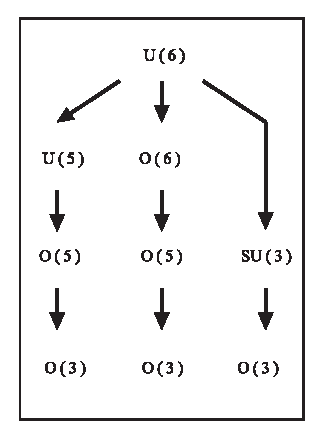
\includegraphics[scale=.65]{figure}
%
% If not, use
%\picplace{5cm}{2cm} % Give the correct figure height and width in cm
%
\caption{If the width of the figure is less than 7.8 cm use the \texttt{sidecapion} command to flush the caption on the left side of the page. If the figure is positioned at the top of the page, align the sidecaption with the top of the figure -- to achieve this you simply need to use the optional argument \texttt{[t]} with the \texttt{sidecaption} command}
\label{fig:1}       % Give a unique label
\end{figure}


\paragraph{Paragraph Heading} %
Instead of simply listing headings of different levels we recommend to let every heading be followed by at least a short passage of text. Furtheron please use the \LaTeX\ automatism for all your cross-references and citations as has already been described in Sect.~\ref{sec:2}.

Please note that the first line of text that follows a heading is not indented, whereas the first lines of all subsequent paragraphs are.

For typesetting numbered lists we recommend to use the \verb|enumerate| environment -- it will automatically render Springer's preferred layout.

\begin{enumerate}
\item{Livelihood and survival mobility are oftentimes coutcomes of uneven socioeconomic development.}
\begin{enumerate}
\item{Livelihood and survival mobility are oftentimes coutcomes of uneven socioeconomic development.}
\item{Livelihood and survival mobility are oftentimes coutcomes of uneven socioeconomic development.}
\end{enumerate}
\item{Livelihood and survival mobility are oftentimes coutcomes of uneven socioeconomic development.}
\end{enumerate}


\subparagraph{Subparagraph Heading} In order to avoid simply listing headings of different levels we recommend to let every heading be followed by at least a short passage of text. Use the \LaTeX\ automatism for all your cross-references and citations as has already been described in Sect.~\ref{sec:2}, see also Fig.~\ref{fig:2}.

Please note that the first line of text that follows a heading is not indented, whereas the first lines of all subsequent paragraphs are.

For unnumbered list we recommend to use the \verb|itemize| environment -- it will automatically render Springer's preferred layout.

\begin{itemize}
\item{Livelihood and survival mobility are oftentimes coutcomes of uneven socioeconomic development, cf. Table~\ref{tab:1}.}
\begin{itemize}
\item{Livelihood and survival mobility are oftentimes coutcomes of uneven socioeconomic development.}
\item{Livelihood and survival mobility are oftentimes coutcomes of uneven socioeconomic development.}
\end{itemize}
\item{Livelihood and survival mobility are oftentimes coutcomes of uneven socioeconomic development.}
\end{itemize}

\begin{figure}[t]
\sidecaption[t]
% Use the relevant command for your figure-insertion program
% to insert the figure file.
% For example, with the option graphics use
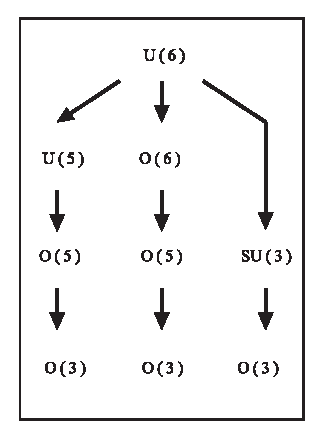
\includegraphics[scale=.65]{figure}
%
% If not, use
%\picplace{5cm}{2cm} % Give the correct figure height and width in cm
%
\caption{Please write your figure caption here}
\label{fig:2}       % Give a unique label
\end{figure}

\runinhead{Run-in Heading Boldface Version} Use the \LaTeX\ automatism for all your cross-references and citations as has already been described in Sect.~\ref{sec:2}.

\subruninhead{Run-in Heading Italic Version} Use the \LaTeX\ automatism for all your cross-refer\-ences and citations as has already been described in Sect.~\ref{sec:2}\index{paragraph}.
% Use the \index{} command to code your index words
%
% For tables use
%
\begin{table}
\caption{Please write your table caption here}
\label{tab:1}       % Give a unique label
%
% For LaTeX tables use
%
\begin{tabular}{p{2cm}p{2.4cm}p{2cm}p{4.9cm}}
\hline\noalign{\smallskip}
Classes & Subclass & Length & Action Mechanism  \\
\noalign{\smallskip}\svhline\noalign{\smallskip}
Translation & mRNA$^a$  & 22 (19--25) & Translation repression, mRNA cleavage\\
Translation & mRNA cleavage & 21 & mRNA cleavage\\
Translation & mRNA  & 21--22 & mRNA cleavage\\
Translation & mRNA  & 24--26 & Histone and DNA Modification\\
\noalign{\smallskip}\hline\noalign{\smallskip}
\end{tabular}
$^a$ Table foot note (with superscript)
\end{table}
%
\section{Section Heading}
\label{sec:3}
% Always give a unique label
% and use \ref{<label>} for cross-references
% and \cite{<label>} for bibliographic references
% use \sectionmark{}
% to alter or adjust the section heading in the running head
Instead of simply listing headings of different levels we recommend to let every heading be followed by at least a short passage of text. Furtheron please use the \LaTeX\ automatism for all your cross-references and citations as has already been described in Sect.~\ref{sec:2}.

Please note that the first line of text that follows a heading is not indented, whereas the first lines of all subsequent paragraphs are.

If you want to list definitions or the like we recommend to use the Springer-enhanced \verb|description| environment -- it will automatically render Springer's preferred layout.

\begin{description}[Type 1]
\item[Type 1]{That addresses central themes pertainng to migration, health, and disease. In Sect.~\ref{sec:1}, Wilson discusses the role of human migration in infectious disease distributions and patterns.}
\item[Type 2]{That addresses central themes pertainng to migration, health, and disease. In Sect.~\ref{subsec:2}, Wilson discusses the role of human migration in infectious disease distributions and patterns.}
\end{description}

\subsection{Subsection Heading} %
In order to avoid simply listing headings of different levels we recommend to let every heading be followed by at least a short passage of text. Use the \LaTeX\ automatism for all your cross-references and citations citations as has already been described in Sect.~\ref{sec:2}.

Please note that the first line of text that follows a heading is not indented, whereas the first lines of all subsequent paragraphs are.

\begin{svgraybox}
If you want to emphasize complete paragraphs of texts we recommend to use the newly defined Springer class option \verb|graybox| and the newly defined environment \verb|svgraybox|. This will produce a 15 percent screened box 'behind' your text.

If you want to emphasize complete paragraphs of texts we recommend to use the newly defined Springer class option and environment \verb|svgraybox|. This will produce a 15 percent screened box 'behind' your text.
\end{svgraybox}


\subsubsection{Subsubsection Heading}
Instead of simply listing headings of different levels we recommend to let every heading be followed by at least a short passage of text. Furtheron please use the \LaTeX\ automatism for all your cross-references and citations as has already been described in Sect.~\ref{sec:2}.

Please note that the first line of text that follows a heading is not indented, whereas the first lines of all subsequent paragraphs are.

\begin{theorem}
Theorem text goes here.
\end{theorem}
%
% or
%
\begin{definition}
Definition text goes here.
\end{definition}

\begin{proof}
%\smartqed
Proof text goes here.
\qed
\end{proof}

\paragraph{Paragraph Heading} %
Instead of simply listing headings of different levels we recommend to let every heading be followed by at least a short passage of text. Furtheron please use the \LaTeX\ automatism for all your cross-references and citations as has already been described in Sect.~\ref{sec:2}.

Note that the first line of text that follows a heading is not indented, whereas the first lines of all subsequent paragraphs are.
%
% For built-in environments use
%
\begin{theorem}
Theorem text goes here.
\end{theorem}
%
\begin{definition}
Definition text goes here.
\end{definition}
%
\begin{proof}
\smartqed
Proof text goes here.
\qed
\end{proof}
%
\begin{acknowledgement}
If you want to include acknowledgments of assistance and the like at the end of an individual chapter please use the \verb|acknowledgement| environment -- it will automatically render Springer's preferred layout.
\end{acknowledgement}
%
\section*{Appendix}
\addcontentsline{toc}{section}{Appendix}
%
When placed at the end of a chapter or contribution (as opposed to at the end of the book), the numbering of tables, figures, and equations in the appendix section continues on from that in the main text. Hence please \textit{do not} use the \verb|appendix| command when writing an appendix at the end of your chapter or contribution. If there is only one the appendix is designated ``Appendix'', or ``Appendix 1'', or ``Appendix 2'', etc. if there is more than one.

\begin{equation}
a \times b = c
\end{equation}
% Problems or Exercises should be sorted chapterwise
\section*{Problems}
\addcontentsline{toc}{section}{Problems}
%
% Use the following environment.
% Don't forget to label each problem;
% the label is needed for the solutions' environment
\begin{prob}
\label{prob1}
A given problem or Excercise is described here. The
problem is described here. The problem is described here.
\end{prob}

\begin{prob}
\label{prob2}
\textbf{Problem Heading}\\
(a) The first part of the problem is described here.\\
(b) The second part of the problem is described here.
\end{prob}

%\input{referenc_1}

\begin{thebibliography}{99}


\bibitem{Lipschutz2007}
S. Lipschutz and M. L. Lipson, \textit{Schaum's Outline of Theory and Problems of Discrete Mathematics}, Third Edition, New York: McGraw-Hill, 2007.

\bibitem{Rosen2007}
K. H. Rosen, \textit{Discrete Mathematics and Its Applications}, Seventh Edition, New York: McGraw-Hill, 2007.

\bibitem{Maclane1988}
S. Maclane and G. Birkhoff, \textit{Algebra}, Third Edition, New York: Bchelsea Publishing Company, 1988.
\end{thebibliography}

%\include{chapter_21}
%\include{chapter_2_function}
%%%%%%%%%%%%%%%%%%%%%% appendix.tex %%%%%%%%%%%%%%%%%%%%%%%%%%%%%%%%%
%
% sample appendix
%
% Use this file as a template for your own input.
%
%%%%%%%%%%%%%%%%%%%%%%%% Springer-Verlag %%%%%%%%%%%%%%%%%%%%%%%%%%

\appendix
\motto{All's well that ends well}
\chapter{Chapter Heading}
\label{introA} % Always give a unique label
% use \chaptermark{}
% to alter or adjust the chapter heading in the running head

Use the template \emph{appendix.tex} together with the Springer document class SVMono (monograph-type books) or SVMult (edited books) to style appendix of your book in the Springer layout.


\section{Section Heading}
\label{sec:A1}
% Always give a unique label
% and use \ref{<label>} for cross-references
% and \cite{<label>} for bibliographic references
% use \sectionmark{}
% to alter or adjust the section heading in the running head
Instead of simply listing headings of different levels we recommend to let every heading be followed by at least a short passage of text. Furtheron please use the \LaTeX\ automatism for all your cross-references and citations.


\subsection{Subsection Heading}
\label{sec:A2}
Instead of simply listing headings of different levels we recommend to let every heading be followed by at least a short passage of text. Furtheron please use the \LaTeX\ automatism for all your cross-references and citations as has already been described in Sect.~\ref{sec:A1}.

For multiline equations we recommend to use the \verb|eqnarray| environment.
\begin{eqnarray}
\vec{a}\times\vec{b}=\vec{c} \nonumber\\
\vec{a}\times\vec{b}=\vec{c}
\label{eq:A01}
\end{eqnarray}

\subsubsection{Subsubsection Heading}
Instead of simply listing headings of different levels we recommend to let every heading be followed by at least a short passage of text. Furtheron please use the \LaTeX\ automatism for all your cross-references and citations as has already been described in Sect.~\ref{sec:A2}.

Please note that the first line of text that follows a heading is not indented, whereas the first lines of all subsequent paragraphs are.

% For figures use
%
\begin{figure}[t]
\sidecaption[t]
%\centering
% Use the relevant command for your figure-insertion program
% to insert the figure file.
% For example, with the option graphics use
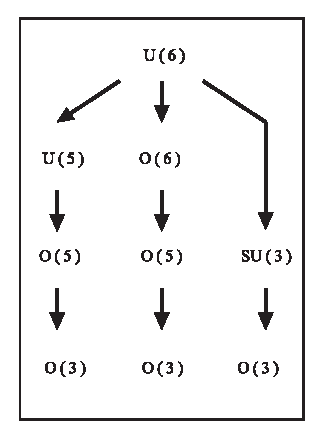
\includegraphics[scale=.65]{figure}
%
% If not, use
%\picplace{5cm}{2cm} % Give the correct figure height and width in cm
%
\caption{Please write your figure caption here}
\label{fig:A1}       % Give a unique label
\end{figure}

% For tables use
%
\begin{table}
\caption{Please write your table caption here}
\label{tab:A1}       % Give a unique label
%
% For LaTeX tables use
%
\begin{tabular}{p{2cm}p{2.4cm}p{2cm}p{4.9cm}}
\hline\noalign{\smallskip}
Classes & Subclass & Length & Action Mechanism  \\
\noalign{\smallskip}\hline\noalign{\smallskip}
Translation & mRNA$^a$  & 22 (19--25) & Translation repression, mRNA cleavage\\
Translation & mRNA cleavage & 21 & mRNA cleavage\\
Translation & mRNA  & 21--22 & mRNA cleavage\\
Translation & mRNA  & 24--26 & Histone and DNA Modification\\
\noalign{\smallskip}\hline\noalign{\smallskip}
\end{tabular}
$^a$ Table foot note (with superscript)
\end{table}
%


%\backmatter%%%%%%%%%%%%%%%%%%%%%%%%%%%%%%%%%%%%%%%%%%%%%%%%%%%%%%%
%\include{glossary}
%
\Extrachap{Solutions}

\section*{Problems of Chapter~\ref{intro}}

\begin{sol}{prob1}
The solution\index{problems}\index{solutions} is revealed here.
\end{sol}


\begin{sol}{prob2}
\textbf{Problem Heading}\\
(a) The solution of first part is revealed here.\\
(b) The solution of second part is revealed here.
\end{sol}


%\printindex

%%%%%%%%%%%%%%%%%%%%%%%%%%%%%%%%%%%%%%%%%%%%%%%%%%%%%%%%%%%%%%%%%%%%%%

$\emph{P}$ $\texttt{P}$ $\P$  $\mathrm{P}$  $\mathcal{P}$ $\mathit{P}$  $\mathnormal{P}$  $\boldsymbol{P}$  $\mathbf{P}$
\\
\\
the signatures of the transition relations:

$T \in P(Q \times V \times Q)$

$T \in V \to P(Q \times Q)$

$T \in Q\times Q \to P(V)$

$T \in Q \times V \to P(Q)$

$T \in Q \to P(V \times Q)$

for example, the function $T \in Q \to P(V \times Q)$ is defined as $T(p) = \{(a,q):(p,a,q) \in T\}$
\\
\\
$\epsilon$-transition relation:

$E \in P(Q\times Q)$

$E \in Q \to P(Q)$
\\
\\
\indent
$T \in P(Q \times V \times Q), T = \{(s,a,q) \}$

$T(s)\in Q \to P(V\times Q), T(s) = \{(a,q):(s,a,q) \in T\}$

According to Convention A.4 (Tuple projection):

$\bar{\pi}_2(T) = \{(s,q): (s,a,q)\in T \}$ 

$\pi_2(T(s)) = \{ q : (s,a,q) \in T\}$  
\\
\\
$f(a)=(f(a^R))^R$

\end{document}


 \chapter{Finite automata minimization algorithms}

\section{Introduction}

\section{Brzozowski's algorithm}

\begin{flushleft}
$\epsilon-free$ FA: $M_0=(Q_0,V,T_0,\emptyset,S_0,F_0)$ \\
to be minimized $DFA$: $M_2=(Q_2,V,T_2,\emptyset,S_2,F_2)$ \\
intermediate $NFA$: $M_1=(Q_1,V,T_1,\emptyset,S_1,F_1)$\\
\end{flushleft}

NFA: $M_1 \to $ DFA: $M_2, M_2=suseful_s\circ subsetopt(M_1)$
\begin{align*}
& q_0,q_1\in Q_1,Q_2\subseteq\mathbb{P}(Q_1),\forall p\in  Q_2,p=(q_0,q_1)\\
& \overrightarrow{L}_{M_2}(p)=\overrightarrow{L}_{M_1}(q_0)\cup  \overrightarrow{L}_{M_1}(q_1)\\
& \Rightarrow \\
& \overrightarrow{L}_{M_2}(p)=\bigcup_{q\in p}\overrightarrow{L}_{M_1}(q)\\
& \Rightarrow 
\end{align*}

\begin{figure}[htbp]
	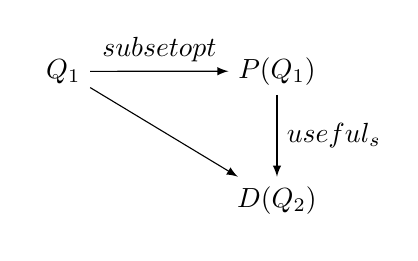
\begin{tikzpicture}
	\matrix (a) [matrix of math nodes,row sep=3em,
	column sep=5em, nodes in empty cells]
	{ Q_1 &  P(Q_1) \\ 
		&  D(Q_2) \\};
	\path[>=latex,->] 
	(a-1-1) edge node [auto] {$subsetopt$} (a-1-2)
	edge node [auto,swap] {$$} (a-2-2)
	(a-1-2) edge node [auto] {$useful_s$} (a-2-2)
	;
	\end{tikzpicture}
	\caption{$M_2=suseful_s\circ subsetopt(M_1)$}
\end{figure}

\begin{figure}[htbp]
	\subfigure[$M_1=(Q_1,V,T_1,\emptyset,S_1,F_1)$] { \label{fig:a} 
	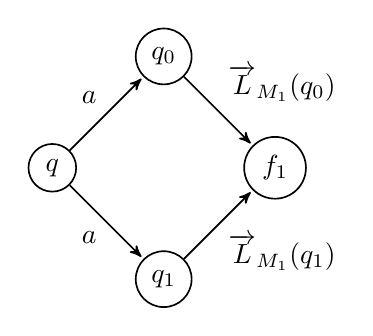
\begin{tikzpicture}[->,>=stealth',shorten >=1pt,auto,node distance=2cm, semithick]
		\tikzstyle{every state}=[minimum size=0.1mm]
		\node[state] (q)  [] {$q$};
		\node[state] (q0) [above right of=q] {$q_0$};
		\node[state] (q1) [below right of=q] {$q_1$};
		\node[state] (f1)  [below right of=q0] {$f_1$};
		\path 
		(q) edge [] node {$a$} (q0)
		    edge [swap] node {$a$} (q1)
		(q0) edge [] node {$\overrightarrow{L}_{M_1}(q_0)$} (f1)
		(q1) edge [swap] node {$\overrightarrow{L}_{M_1}(q_1)$} (f1)
		;
	\end{tikzpicture}
    }
    \hspace{2cm}
	\subfigure[$M_2=(Q_2,V,T_2,\emptyset,S_2,F_2)$] { \label{fig:b}
    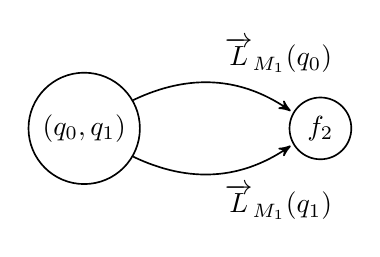
\begin{tikzpicture}[->,>=stealth',shorten >=1pt,auto,node distance=3cm, semithick,scale=4]
    	\tikzstyle{every state}=[minimum size=0.1mm]
    	\node[state] (q01)  {$(q_0,q_1)$};
    	\node[state] (f2)  [right of=q01] {$f_2$};
    	\path 
    	(q01) edge [bend left] node {$\overrightarrow{L}_{M_1}(q_0)$} (f2)
    	(q01) edge [bend right,swap] node {$\overrightarrow{L}_{M_1}(q_1)$} (f2)
    	;
    \end{tikzpicture}
    }
	\caption{$M_2=suseful_s\circ subsetopt(M_1)$}
\end{figure}

\begin{figure}[htbp]
	\subfigure[$M_0=(Q_0,V,T_0,\emptyset,S_0,F_0)$] {
		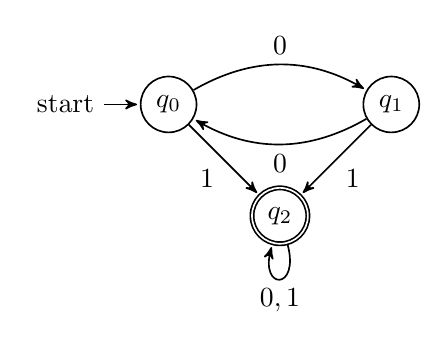
\begin{tikzpicture}[->,>=stealth',shorten >=1pt,auto,node distance=2cm, semithick]
		\tikzstyle{every state}=[minimum size=0.1mm]
		\node[state,accepting] (q2) []{$q_2$};
		\node[state,initial] (q0) [above left of=q2] {$q_0$};
		\node[state] (q1) [above right of=q2] {$q_1$};
		\path
		(q0) edge[bend left] node {$0$} (q1)
		(q1) edge[bend left] node {$0$} (q0)
		(q0) edge[swap] node {$1$} (q2)
		(q1) edge[] node {$1$} (q2)
		(q2) edge[loop below] node {$0,1$} (q2)
		;
		\end{tikzpicture}
	}
    \hspace{1cm}
	\subfigure[$M^R_0=(Q_0,V,T_0,\emptyset,S_0,F_0)^R=(Q_0,V,T^R,\emptyset,F_0,S_0)$]{
		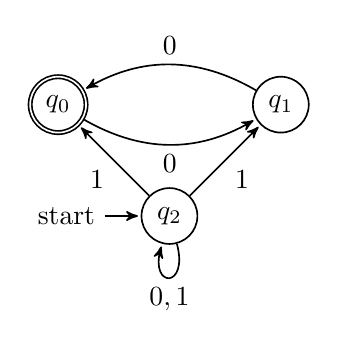
\begin{tikzpicture}[->,>=stealth',shorten >=1pt,auto,node distance=2cm, semithick]
		\tikzstyle{every state}=[minimum size=0.1mm]
		\node[state,initial] (q2) []{$q_2$};
		\node[state,accepting] (q0) [above left of=q2] {$q_0$};
		\node[state] (q1) [above right of=q2] {$q_1$};
		\path
		(q1) edge[bend right,swap] node {$0$} (q0)
		(q0) edge[bend right,swap] node {$0$} (q1)
		(q2) edge[] node {$1$} (q0)
		(q2) edge[swap] node {$1$} (q1)
		(q2) edge[loop below] node {$0,1$} (q2)
		;
		\end{tikzpicture}
	}
    \newline
	\subfigure[$useful_s\circ subsetopt\circ R(M_0)$]{
		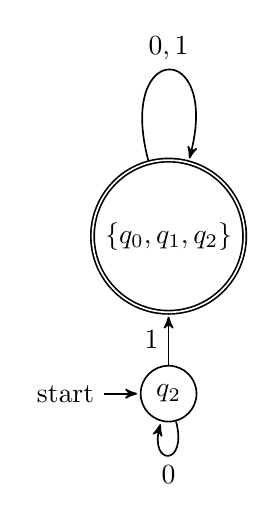
\begin{tikzpicture}[->,>=stealth',shorten >=1pt,auto,node distance=2cm, semithick]
		\tikzstyle{every state}=[minimum size=0.1mm]
		\node[state,initial] (q2) []{$q_2$};
		\node[state,accepting] (q0) [above of=q2] {$\{q_0,q_1,q_2\}$};
		\path
		(q2) edge[] node {$1$} (q0)
		(q0) edge[loop above] node {$0,1$} (q0)
		(q2) edge[loop below] node {$0$} (q2)
		;
	\end{tikzpicture}
	}
    \hspace{3cm}
    \subfigure[$M_1=R\circ useful_s\circ subsetopt\circ R(M_0)$]{
    	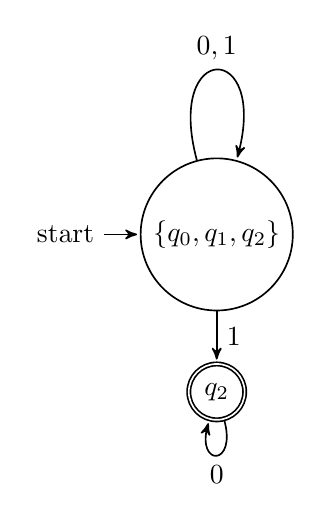
\begin{tikzpicture}[->,>=stealth',shorten >=1pt,auto,node distance=2cm, semithick]
    	\tikzstyle{every state}=[minimum size=0.1mm]
    	\node[state,accepting] (q2) []{$q_2$};
    	\node[state,initial] (q0) [above of=q2] {$\{q_0,q_1,q_2\}$};
    	\path
    	(q0) edge[] node {$1$} (q2)
    	(q0) edge[loop above] node {$0,1$} (q0)
    	(q2) edge[loop below] node {$0$} (q2)
    	;
    	\end{tikzpicture}
    }
    \caption{$M_1=R\circ useful_s\circ subsetopt\circ R(M_0)$}
\end{figure}

\begin{figure}[htbp]
	\begin{align*}
	\text{start: } &U=\{q_2\},D=\emptyset \\
	u=q_2: & T(q_2,0)=\{q_2\},T(q_2,1)=\{q_0,q_1,q_2\} \\
	&\text{add new state to $D$, } D=\{q_2,\{q_0,q_1,q_2\}\} \\
	u=\{q_0,q_1,q_2\}:& T(\{q_0,q_1,q_2\},0)=T(q_0,0)\cup T(q_1,0)\cup T(q_2,0)=\{q_1\}\cup \{q_0\}\cup \{q_2\} =\{q_0,q_1,q_2\}\\
	&T(\{q_0,q_1,q_2\},1)=T(q_0,1)\cup T(q_1,1)\cup T(q_2,1)=\emptyset\cup \emptyset \cup \{q_0,q_1,q_2\}=\{q_0,q_1,q_2\}
	\end{align*}
	
	\subfigure[$M$]{
		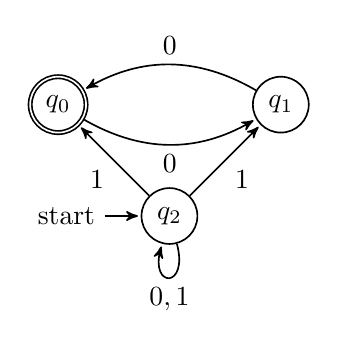
\begin{tikzpicture}[->,>=stealth',shorten >=1pt,auto,node distance=2cm, semithick]
		\tikzstyle{every state}=[minimum size=0.1mm]
		\node[state,initial] (q2) []{$q_2$};
		\node[state,accepting] (q0) [above left of=q2] {$q_0$};
		\node[state] (q1) [above right of=q2] {$q_1$};
		\path
		(q1) edge[bend right,swap] node {$0$} (q0)
		(q0) edge[bend right,swap] node {$0$} (q1)
		(q2) edge[] node {$1$} (q0)
		(q2) edge[swap] node {$1$} (q1)
		(q2) edge[loop below] node {$0,1$} (q2)
		;
		\end{tikzpicture}
	}
    \hspace{2cm}
	\subfigure[$useful_s\circ subsetopt(M)$]{
		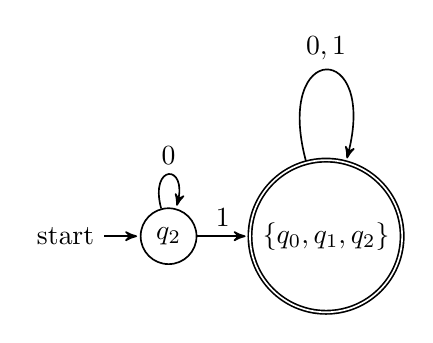
\begin{tikzpicture}[->,>=stealth',shorten >=1pt,auto,node distance=2cm, semithick]
		\tikzstyle{every state}=[minimum size=0.1mm]
		\node[state,initial] (q2) []{$q_2$};
		\node[state,accepting] (q0) [right of=q2] {$\{q_0,q_1,q_2\}$};
		\path
		(q2) edge[] node {$1$} (q0)
		(q0) edge[loop above] node {$0,1$} (q0)
		(q2) edge[loop above] node {$0$} (q2)
		;
		\end{tikzpicture}
	}
	\caption{$useful_s\circ subsetopt(M)$}
\end{figure}

\section{Minimization by equivalence of states}

\begin{figure}[htbp]
	Equivalence relation $E\subseteq Q\times Q$\\
	$(p,q)\in E\equiv (\overrightarrow{L}(p)=\overrightarrow{L}(q))$\\
	
	\subfigure[$(p,q)\in E$]{
		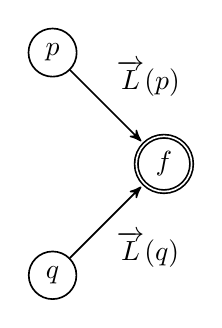
\begin{tikzpicture}[->,>=stealth',shorten >=1pt,auto,node distance=2cm, semithick]
		\tikzstyle{every state}=[minimum size=0.1mm]
		\node[state,accepting] (f) {$f$};
		\node[state] (p) [above left of=f]{$p$};
		\node[state] (q) [below left of=f]{$q$};
		\path
		(p) edge[] node {$\overrightarrow{L}(p)$} (f)
		(q) edge[swap] node {$\overrightarrow{L}(q)$} (f)
		;
		\end{tikzpicture}
		}
	    \hspace{2cm}
    	\subfigure[$(p,q)\in E$]{
    	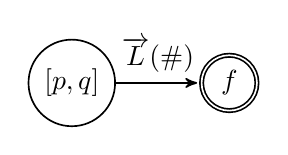
\begin{tikzpicture}[->,>=stealth',shorten >=1pt,auto,node distance=2cm, semithick]
    	\tikzstyle{every state}=[minimum size=0.1mm]
    	\node[state,accepting] (f) {$f$};
    	\node[state] (p) [left of=f]{$[p,q]$};
    	\path
    	(p) edge[] node {$\overrightarrow{L}(\#)$} (f)
    	;
    	\end{tikzpicture}
   		}
	\caption{Equivalence relation $E\subseteq Q\times Q$}
\end{figure}

\begin{figure}[htbp]
	$\overrightarrow{L}(p)=\bigcup_{a\in V}(\{a\} \cdot \overrightarrow{L}(T(p,a)) \cup \{\epsilon|p\in F\}$\\

	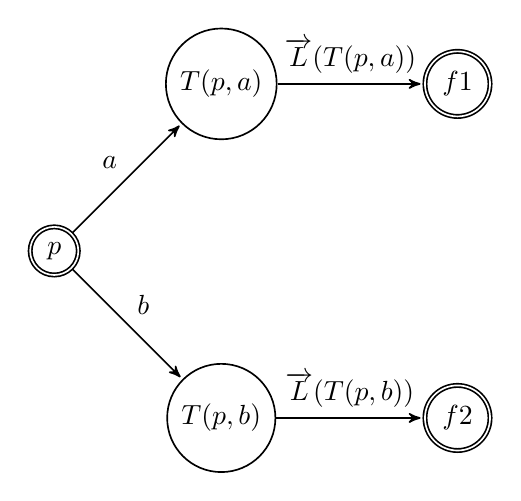
\begin{tikzpicture}[->,>=stealth',shorten >=1pt,auto,node distance=3cm, semithick]
		\tikzstyle{every state}=[minimum size=0.1mm]
		\node[state,accepting] (p) {$p$};
		\node[state] (q1) [above right of=p]{$T(p,a)$};
		\node[state] (q2) [below right of=p]{$T(p,b)$};
		\node[state,accepting] (f1) [right of=q1]{$f1$};
		\node[state,accepting] (f2) [right of=q2]{$f2$};
		\path
		(p) edge[] node {$a$} (q1)
		(p) edge[] node {$b$} (q2)
		(q1) edge[] node {$\overrightarrow{L}(T(p,a))$} (f1)
		(q2) edge[] node {$\overrightarrow{L}(T(p,b))$} (f2)
		;
	\end{tikzpicture}
	\caption{$L(p)$}
\end{figure}

Let $A=(Q,V,T,_,F)$ be a deterministic finite automaton, where $Q$ is a finite set of states, $V$ is a finite set of input symbols, $T$ is a mapping from $Q\times V$ into $Q$, and $F\subseteq Q$ is the set of final states. No initial state is specified since it is of no importance in what follows. The mapping $T$ is extended to $T\times V^\ast$ in the usual manner where $V^\ast$ denotes the set of all finite strings (including the empty string $\epsilon$) of symbols from $V$

\begin{definition}[equivalent states]
	The states $s$ and $t$ are said to be equivalent if for each $x\in V^\ast, T(s,x)\in F$ if and only if $T(t,x)\in F$. 
\end{definition}

\begin{figure}[htbp]
	a: $((T(p,a),T(q,a))\in E_0$; b: $((T(p,a),T(q,a))\notin E_0$, c: $((T(p,a),T(q,a))\in E_1(part_1)$; d: $((T(p,a),T(q,a))\notin E_1(part_1)$;\\
	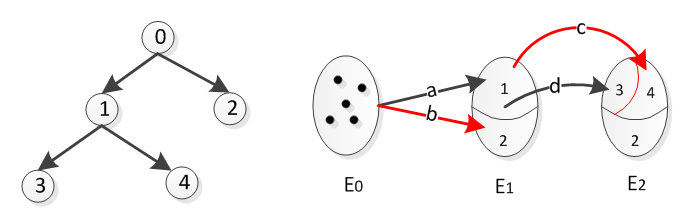
\includegraphics[scale=0.8]{approximatingE}
	\caption{Approximating $E, E_0=(Q\setminus F)^2\cup F^2$ }
\end{figure}

\begin{figure}[htbp]
	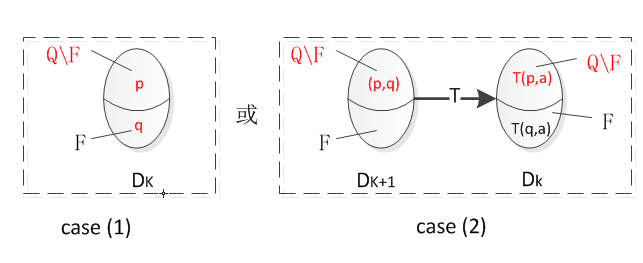
\includegraphics[scale=0.8]{approximatingD}
	\caption{Approximating $D, D_0=((Q\setminus F)\times F)\cup (F\times (Q\setminus F))$ }
\end{figure}

\begin{figure}[htbp]
	initial,$P=[Q]_{E_0}=\{F,Q\setminus F\},Q_0,Q_1\in P$, \\
	if ($\exists p,q\in Q_0,T(p,a)\in Q_1$, and  $T(q,a)\notin Q_1$), then \\
	split $Q_0$ wrt ($Q_1,a$) $\to$ two parts, (1): $Q_0^\prime\in Q_1$ and (2): $(Q_0\setminus Q_0^\prime)\notin Q_1$ \\
	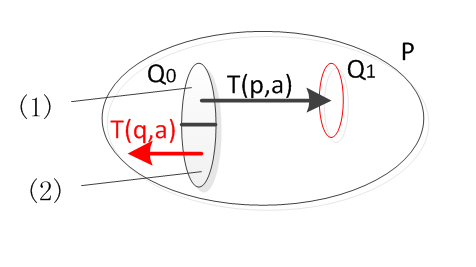
\includegraphics[scale=0.8]{splittable}
	\caption{split $Q_0$ wrt $Q_1$ }
\end{figure}

\section{From \cite{Gries73}}

\subsection{Problem Definition}

DFA: $A=(S,I,\delta,F)$, No initial state is specified since it is of no importance in what follows.

\begin{definition}[equivalent states]
	States $s$ and $t$ are said to be equivalent if for each $x\in I^\ast,\delta(s,x)\in F$. if and only if $\delta(t,x)\in F$.
\end{definition}

We want an algorithm which finds equivalent states of a finite automaton.

\begin{example}
	Consider the automaton with $S=\{a,b,c,d,e\},I=\{0,1\},F=\{d,e\}$ and $\delta$ is given by the arc of diagram of Fig. \ref{fig:ex}.
\begin{figure} [htbp]
	\{a,b\},\{d,e\}is not equivalent states. \\
	Sets of equivalent states: \{a,c\},\{b\},\{d\},\{e\}\\
	%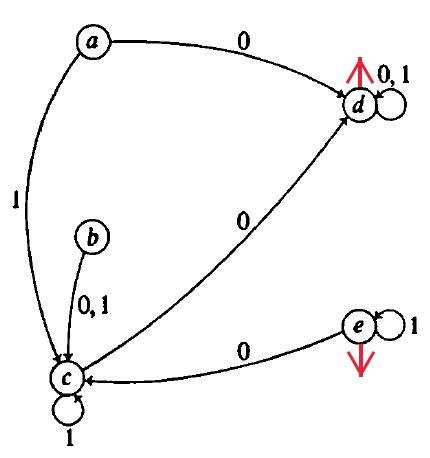
\includegraphics[scale=0.4] {mini-fa} 
	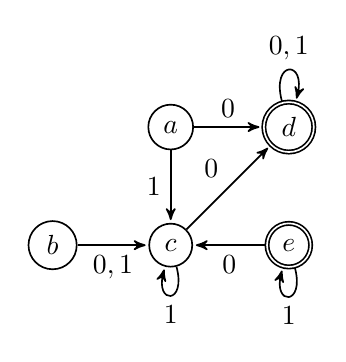
\begin{tikzpicture}[->,>=stealth',shorten >=1pt,auto,node distance=1.5cm, semithick]
	\tikzstyle{every state}=[minimum size=0.1mm]
	\node[state] (a) {$a$};
	\node[state,accepting] (d) [right of=a] {$d$};
	\node[state] (c) [below of=a] {$c$};
	\node[state] (b) [left of=c] {$b$};
	\node[state,accepting] (e) [right of=c] {$e$};
	\path
	(d) edge [loop above] node {$0,1$} (d)
	(c) edge [loop below] node {$1$} (c)
	(e) edge [loop below] node {$1$} (e)
	(a) edge [] node {$0$} (d)
	(a) edge [swap] node {$1$} (c)
	(b) edge [swap] node {$0,1$} (c)
	(e) edge [] node {$0$} (c)
	(c) edge [] node {$0$} (d)
	;
	\end{tikzpicture}
	\caption{Finite state automaton}
	\label{fig:ex}
\end{figure}
\end{example}

\subsection{The Basic Algorithm}
\begin{definition}[acceptable partition]
	A partitioning of the states into blocks $B_1,B_2,\dots,B_p$ is acceptable if (a) no block contains both a final and a nonfinal state, and (b) if $s$ and $t$ are equivalent states then they are in the same block.
\end{definition}

\begin{lemma} \label{lem:partitioning}
	The partitioning $B_1=F,B_2=S-F$ is acceptable.
\end{lemma}

\begin{lemma} \label{lem:stSame}
	The partitioning $B_1,B_2,\dots,B_p$ gives the blocks of equivalent states if and only if (a) the partitioning is acceptable and (b) for each pair of blocks $B_i,B_j$ and symbol $a\in I$
	\begin{equation}
	s,t\in B_i,\delta(s,a)\in B_j \text{ implies } \delta(t,a)\in B_j
	\end{equation}
\end{lemma}

\begin{lemma} \label{lem:split}
	Let $B_1,B_2,\dots,B_p$ be an acceptable partitioning. Suppose there are two blocks $B_i,B_j$ and symbol $a\in I$ such that
	\begin{equation}
	s,t\in B_i,\delta(s,a)\in B_j \text{ but } \delta(t,a)\notin B_j
	\label{eq:split}
	\end{equation}
	
	Then $s$ and $t$ are not equivalent states, and we get a new acceptable partitioning by replacing $B_i$ by the two blocks
	\begin{equation}
	\{s\in B_i|\delta(s,a)\in B_j\} \text{ and } \{s\in B_i|\delta(s,a)\notin B_j\}
	\end{equation}
\end{lemma}

This splitting of $B_i$ as described is called splitting $B_i$ with respect to the pair $(B_i, a)$ or simply splitting $B_i$ wrt $(B_j, a)$. We now write the following algorithm:

\begin{algorithm}  
	\caption{splitting $B_i$ wrt $(B_j, a)$} 
	\label{alg:splitting} 
	\begin{algorithmic}%[1] %每行显示行号
	\State $B_1 \gets F; B_2\gets S-F;$  [initially there are two blocks]  
	\While { $\exists a,B_i,B_j $ such that Eq. (\ref{eq:split}) holds }
		\State SPLIT: split $B_i$ wrt $(B_j,a)$
	\EndWhile
	\end{algorithmic}   
\end{algorithm}

$B$,$P$ are relations, $S$ is a sequence of statements.
\begin{equation}
	P\land B\{S\}P \text{ implies $P$ \{While $B$ do $S$ end\} } P\land\lnot B
\end{equation}

For algorithm (\ref{alg:splitting}), let $P$ be the relation ``the partitioning is acceptable". By Lemma \ref{lem:partitioning}, $P$ is true just before execution of the while loop, while by Lemma \ref{lem:split} execution of $S$ always yields an acceptable partitioning. The relation $B$ is ``$\exists a,B_i,B_j such that  Eq. (\ref{eq:split}) holds $". Thus, $P$ and $\lnot B$ hold after execution of the loop, but these are the sufficient requirements described in Lemma \ref{lem:stSame} for the final partitioning to be the described one.

Our refinement (\ref{alg:refinement}) determines all splittings wrt a pair $(B_i, a)$ and then performs all these splittings at the same time.
\begin{algorithm}  
	\caption{splitting $B_i$ wrt $(B_j, a)$} 
	\label{alg:refinement} 
	\begin{algorithmic}%[1] %每行显示行号
		\State $B_1 \gets F; B_2\gets S-F;$  [initially there are two blocks]  
		\While { $\exists a,B_i,B_j $ such that Eq. (\ref{eq:split}) holds }
		\State Determine the splittings of all blocks wrt $(B_j,a)$
		\State Split each block as just determined.
		\EndWhile
	\end{algorithmic}   
\end{algorithm}

The algorithm is not very efficient, it's $|I||S|^2$.

The result of splitting all blocks wrt $(B_j, a)$ is that any future block $B$ (including the final blocks) satisfies one of the following:

\begin{align}
&\text{(a) for all } s\in B\quad \delta(s,a)\in B_j, \text{ or } \label{eq:splitB} \\
&\text{(b) for all } s\in B\quad \delta(s,a)\notin B_j \notag %无编号
\end{align}

\begin{lemma} 
	Suppose all blocks have been split wrt $(B_j, a)$. Then there is no need to split any future block wrt $(B_j, a)$.
\end{lemma}

\begin{lemma} \label{lem:three_pairs}
Suppose a block $B_j$ is split into blocks $\bar{B}_j$ and $\tilde{B}_j$. Consider a symbol $a$. Splitting all blocks wrt to any two of the three pairs $(B_j, a), (\bar(B)_j, a)$, and $(\tilde{B}_j, a)$ performs the same function as splitting all blocks wrt all three pairs.
\end{lemma}

\begin{proof}
	Suppose we split all blocks wrt $(B_j, a)$ and $(\bar{B}_j, a)$. This implies that each future block $B$ satisfies one of the following:
	\begin{align*}
    & s\in B \text{ implies } \delta(s,a)\in B_j \text{ and } \delta(s,a)\in \bar{B}_j, \text{ or } \\
    & s\in B \text{ implies } \delta(s,a)\in B_j \text{ and } \delta(s,a)\notin \bar{B}_j, \text{ or } \\
    & s\in B \text{ implies } \delta(s,a)\notin B_j \text{ and } \delta(s,a)\notin \bar{B}_j, \text{ or } \\
    & s\in B \text{ implies } \delta(s,a)\notin B_j \text{ and } \delta(s,a)\in \bar{B}_j
	\end{align*}
	Since $\bar{B}_j\cup\tilde{B}_j=B_j$ and $\bar{B}_j\cap\tilde{B}_j=\emptyset$, we infer that one of the following holds:
	\begin{align*}
	& s\in B \text{ implies } \delta(s,a)\in \tilde{B}_j, \text{ or } \\
	& s\in B \text{ implies } \delta(s,a)\notin \tilde{B}_j
	\end{align*}
	This is precisely what splitting all blocks wrt $(\tilde{B}_j,a)$ accomplishes (see (\ref{eq:splitB})). We leave to the reader to prove the rest of the theorem (in the same fashion)--that	splitting wrt $(\bar{B}_j,a)$ and $(\tilde{B}_j,a)$ accomplishes the task of splitting wrt $(B_j, a)$; and that splitting wrt $(B_j, a)$ and $(\tilde{B}, a)$ accomplishes the task of splitting wrt  $(\bar{B}, a)$. $\hfill\square$
\end{proof}

\begin{lemma}
	Let the two initial blocks be $B_1=F$ and $B_2=S-F$. For a given
	symbol $a$, it is necessary to split all blocks wrt only one of the pairs $(B_1, a)$ and $(B_2, a)$.
\end{lemma}

\begin{proof}
	Consider Lemma \ref{lem:three_pairs}, with $B_j=S, \bar{B}_j =F, and \tilde{B}_j=S-F$. We already know that $(s, a)\in B_j$ for any symbol $a$, so it is not necessary to split wrt $(B_j, a)$.
	Hence we need only split wrt either $(\bar{B}_j, a)$ or $(\tilde{B}_j, a)$, but not both. $\hfill\square$
\end{proof}

Let us consider the possibility of maintaining a list $L$ of all pairs $(B_j, a)$ wrt which some blocks may have to be split. Another way to put it is that if we know it is not necessary to split any $B$ (including $B_j$ itself) wrt a pair $(B_j, a)$ we won't put that pair on the list. We can then keep splitting until the list $L$ becomes empty.

see Algorithm \ref{alg:refinement-list}, It remains to show that execution time is no worse than proportional to $|I||S|\log(|S|)$.

\begin{algorithm}  
	\caption{splitting $B_i$ wrt $(B_j, a)$} 
	\label{alg:refinement-list} 
	\begin{algorithmic}%[1] %每行显示行号
		\State $B_1 \gets F; B_2\gets S-F; L=\emptyset$  [initially there are two blocks]  
		\ForAll { $c\in I$ }
			\If {$B_1$ is smaller than $B_2$}
				\State $add(B_1,c)$ to $L$
			\Else
				\State $add(B_2,c)$ to $L$
	        \EndIf
		\EndFor
		
		\While {$L\ne\emptyset$}
			\State b: Pick one pair $(B_j,a)\in L$;
			\State c: Determine splittings of all blocks wrt $(B_j,a)$;
			\State d: $L\gets L-(B_j,a)$;
			\State e: Split each block as determined in $c$;
			\State f: /* Fix $L$ according to the splits that occurred in step e */
			\ForAll {block $B$ just split into $\bar{B}$ and $\tilde{B}$(say) }
				\ForAll { $c\in I$ }
					\If {$(B,c)\in L$ }
						\State $L\gets L+(\bar{B},c)+(\tilde{B},c)-(B,c)$
					\Else
						\If {$\bar{B}$ is smaller than $\tilde{B}$}
							\State $add(\bar{B},c)$ to $L$
						\Else
							\State $add(\tilde{B},c)$ to $L$
						\EndIf
					\EndIf
				\EndFor
			\EndFor
		\EndWhile
	\end{algorithmic}   
\end{algorithm}

Meaning of List $L$. $L$ is a list of pairs $(B_j, a)$ wrt which we must attempt to split all blocks so that either \ref{eq:splitB}(a) or (b) will hold for each block. If $B_j$ is a block and $(B_j, a)\notin L$ for some $a$, then either \ref{eq:splitB}(a) or (b) already holds, or we are assured by other means that either \ref{eq:splitB}(a) or (b) will hold when the algorithm terminates.

Let us now look closer at splitting. Splitting a block $B_i$ wrt $(B_j,a)$ replaces $B_i$ by two blocks $\bar{B}_i$ and $\tilde{B}_i$ which satisfy:
\begin{align*}
& s\in\bar{B}_i \text{  implies  } \delta(s,a)\in B_j \\
& s\in\tilde{B}_i \text{  implies  } \delta(s,a)\notin B_j 
\end{align*}
Given block $B_i$ let us split it by removing from it those states s such that $\delta(s,a)\in B_j$, and putting these states in a new block $B_k$, called $B_i$'s twin. Thus $B_i$ is split into $B_i$ and $B_k$.

In order to determine the splitting of all blocks wrt $(B_j, a)$, we need to make a list $D$ (say) of all states which must be removed from blocks--which satisfy the property $\delta(s,a)\in B_j$. Statement c thus looks like (algorithm \ref{alg:determine}):
\begin{algorithm}  
	\caption{c: Determine the splittings of all blocks wrt $(B_i, a)$} 
	\label{alg:determine} 
	\begin{algorithmic}%[1] %每行显示行号
		\State $D\gets\emptyset$
		\For { each $s\in B_j$}
			\If {$\delta^{-1}(s,a)\ne\emptyset$}
				\State $D\gets D\cup\delta^{-}(s,a)$
			\EndIf
		\EndFor
	\end{algorithmic}   
\end{algorithm}

Statement e, which actually splits blocks, could be written as (algorithm \ref{alg:splitBlocks}):
\begin{algorithm}  
	\caption{e:Split each block as determined in statement c} 
	\label{alg:splitBlocks} 
	\begin{algorithmic}%[1] %每行显示行号
		\For { each block $B_i$ in the partition }
			\State $B_k\gets B_i\cap D$; ($B_k$ is a newly generated block -- $B_i$'s twin)
			\State $B_i\gets B_i-B_k$;
		\EndFor
	\end{algorithmic}   
\end{algorithm}

While correct, statement e is too inefficient since each time it is executed it must manipulate each block, and this would lead to a $|I||S|^2$ algorithm. 

Hence we must refine e further to look only at blocks which have a chance of being partitioned -- which contain states in $D$. We can also recognize a case where removing states is unnecessary. If for all $s\in B,\delta(s,a)\in B_j$ then $\{s\in B_i|\delta(s,a)\notin B_j \}$ is empty. We end up with the following algorithm e:

\begin{algorithm}  
	\caption{e: Split each block as just determined} 
	\label{alg:splitBlocks_refine} 
	\begin{algorithmic}%[1] %每行显示行号
		\State $BI\gets$ block number in which $s$ appears;
		\If {all $s\in BI$ have $\delta(s,a)\in B_j$ }
			\State  [no need to split block--do nothing]
		\Else 
			\If {$BI$ has no twin $BK$ yet}
				\State generate $BI$'s twin $BK$ and set $BK\gets\emptyset$
			\Else
				\State Move $s$ from $BI$ to its twin $BK$
			\EndIf
		\EndIf
	\end{algorithmic}   
\end{algorithm}

Two important ideas helped us in reducing the running time to $mn\log (n)$. The first was that if a block $B$ is split into $\bar{B}$ and $\tilde{B}$ we need only split wrt two of the three pairs $(B, a)$, $(\bar{B}, a)$, and $(\tilde{B}, a)$. The second was that in case we need put only one of $(\bar{B}, a)$ and $(\tilde{B}, a)$ in $L$, we should put the one whose block ($\bar{B}$ or $\tilde{B}$) contains the fewest number of states.

\section{From \cite{Hopcroft71}}

The algorithm for finding the equivalence classes of Q is described below:

\begin{algorithm}  
	\caption{The algorithm for finding the equivalence classes of Q}  
	\begin{algorithmic}%[1] %每行显示行号  
		\Require $M=(Q,V,T,\_,F)$  
		\Ensure The equivalence classes of $Q$  
		\State Step 1. For each $s\in Q$ and each $a\in V$ construct
		
		$T^{-1}(s,a)=\{t|T(t,a)=s\}$ \qquad 计算状态s的in-transitionsss
		
		\State Step 2. construct $B(1)=F, B(2)=Q-F$ and for each $a\in V$ and $1\le i\le 2$ construct
		
		\For{each $a\in V$ }
			\For{$i=1$; $i<n$; $i++$ }  
				\State $\hat{B}(B(i),a)=\{s|s\in B(i) \text{ and } T^{-1}(s,a)\ne \emptyset\}$;
			\EndFor  
		\EndFor 
		\State Step 3. Set $k=3$;
		\State Step 4. For each $a\in V$ construct $L(a)$
		\For{each $a\in V$ }
			\If {$|\hat{B}(B(1),a)| \le |\hat{B}(B(2),a)|$}
				\State $L(a) = \hat{B}(B(1),a)$;
			\Else
	            \State $L(a) = \hat{B}(B(2),a)$; 
			\EndIf
		\EndFor
		\State Step 5. Select $a\in V$ and $i\in L(a)$. The algorithm terminates when $L(a)=\emptyset$ for each $a\in V$.
		\State Step 6. Delete $i$ from $L(a)$.
		\State Step 7. For each $j<k$ such that there exists $t\in B(j)$ with $T(t,a)\in \hat{B}(B(i),a)$, perform steps 7a,7b,7c, and 7d.
		
		\State Step 7a. partition $B(j)$ into
			
			$B^\prime(j)=\{t|T(t,a)\in \hat{B}(B(i),a)\}$ and			
		
			$B^{\prime\prime}(j)=B(j)-B^\prime(j)$
		
		\State Step 7b. Replace $B(j)$ by $B^\prime(j)$ and constant $B(k)=B^{\prime\prime}$. Construct the corresponding $\hat{B}(B(j),a)$ and $\hat{B}(B(k),a)$ for each $a\in V$.
		
		\State Step 7c. For each $a\in V$ modify $L(a)$ as follows.
			\If{$j\notin L(a) \& 0<|\hat{B}(B(j),a)|\le |\hat{B}(B(k)),a|$}
				\State $L(a) = L(a)\cup \{j\}$;
			\Else
				\State $L(a) = L(a)\cup \{k\}$;
			\EndIf 
			
		\State Step 7d. Set $k=k+1$.
		
		\State Step 8. Return to Step 5.
	\end{algorithmic}   
\end{algorithm}

\begin{example}
	$Q=\{1,2,3,4,5,6\},V=\{0,1\},T $ see Fig. \ref{fig:mini-ex1}
	
	The algorithm for finding the equivalence classes of Q is described below: 
	\begin{enumerate}[Step 1. ]
		\item For each $s\in Q$ and each $a\in V$ construct   $T^{-1}(s,a)=\{t|T(t,a)=s\}$\\
			$T^{-1}(1,0)=\emptyset,T^{-1}(2,0)=\{1\},T^{-1}(3,0)=\{2\},\cdots,T^{-1}(6,0)=\{5\}$\\
			$T^{-1}(1,1)=\{1\},T^{-1}(2,1)=\{2\},\cdots T^{-1}(6,1)=\{6\},$
		\item $B(1)=F=\{6\},B(2)=Q-F=\{1,2,3,4,5\}$\\
			for each $a\in V$ and $i\in[1,2]$ construct  $\hat{B}(B(i),a)=\{s|s\in B(i) \text{ and } T^{-1}(s,a)\ne \emptyset\}$;\\
			$\hat{B}(B(1),0)=\{6\},\hat{B}(B(2),0)=\{2,3,4,5\}$ \\
			$\hat{B}(B(1),1)=\{6\},\hat{B}(B(1),1)=\{1,2,3,4,5\}$ 
		\item Set $k=3$
		\item For each $a\in V$ construct $L(a)$ \\
			$L(0) = \{6\},$ \qquad since $|\hat{B}(B(1),0)|=1\le |\hat{B}(B(2),0)|=4$.\\
			$L(1) = \{6\},$ \qquad since $|\hat{B}(B(1),1)|=1\le |\hat{B}(B(2),1)|=5$.
		\item Select $a\in V$ and $i\in L(a)$. The algorithm terminates when $L(a)=\emptyset$ for each $a\in V$.\\
		    $a=0$\\
		    $i=1,\hat{B}(B(i),0)=\{6\}$
		\item Delete $i$ From $L(a)$.\\
			$L(0)=L(0)-B(i)=\emptyset$
		\item For each $j<k$ such that there exists $t\in B(j)$ with $T(t,a)\in \hat{B}(B(i),a)$, perform steps 7a,7b,7c, and 7d. 
			\begin{enumerate}[Step 7a. ]
				\item Partition $B(j)$ into\\ 
					$B^\prime(j)=\{t|T(t,a)\in \hat{B}(B(i),a)\}=\{5\}$ and\\			
				    $B^{\prime\prime}(j)=B(j)-B^\prime(j)$\\
				\item
			\end{enumerate}
	\end{enumerate}  
\end{example}

\begin{figure}[htbp]
	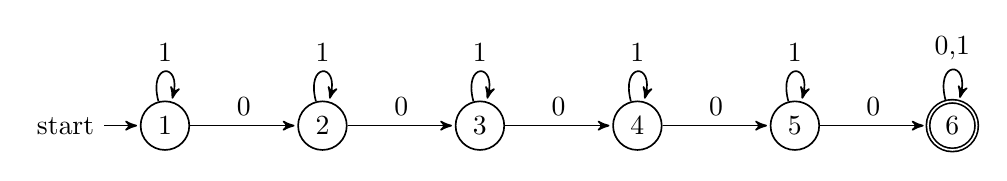
\begin{tikzpicture}[->,>=stealth',shorten >=1pt,auto,node distance=2cm, semithick]
	\tikzstyle{every state}=[minimum size=0.1mm]
	\node[initial,state] (p1)  {$1$};
	\node[state]         (p2) [right of=p1] {$2$};
	\node[state]         (p3) [right of=p2] {$3$};
	\node[state]         (p4) [right of=p3] {$4$};
	\node[state]         (p5) [right of=p4] {$5$};
	\node[state,accepting] (p6) [right of=p5] {$6$};
	\path
	(p1) edge [loop above] node {1} (p1)
	     edge [] node {0} (p2)
	(p2) edge [loop above] node {1} (p2)
	     edge [] node {0} (p3)
	(p3) edge [loop above] node {1} (p3)
		 edge [] node {0} (p4)
    (p4) edge [loop above] node {1} (p4)
         edge [] node {0} (p5)
    (p5) edge [loop above] node {1} (p5)
         edge [] node {0} (p6)
    (p6) edge [loop above] node {0,1} (p6)
	;
	\end{tikzpicture}
	\caption{Minimizing example} \label{fig:mini-ex1}
\end{figure}

\begin{example}
	Consider the automaton with $Q=\{a,b,c,d,e\},V={0,1},F=\{d,e\}$, and $T$ is given by the arcs of diagram of Fig. (\ref{fig:mini-ex2}).
	
	\{a,b\} is not equivalent, since $T(a,0)\in F$ but $T(b,0)\notin F$.
	
	\{d,e\} is not equivalent, since $T(d,0)\in F$ but $T(e,0)\notin F$. 
	
	Sets of equivalent states: \{a,c\},\{b\},\{d\},\{e\}
	
	另外一种描述:
	\begin{enumerate}
		\item $(a,b)\notin E$, since $T(a,0)\in F$ but $T(b,0)\notin F$.
		\item $(d,e)\notin E$, since $T(d,0)\in F$ but $T(e,0)\notin F$.
		\item 	$(a,c)\in E$, since	$(a,c)\in E\equiv(a\in F\equiv c\in F)\land (\forall v\in V,(T(a,v),T(c,v)\in E)$ \\
		$(a\notin F,c\notin F)\Rightarrow (a\in F\equiv c\in F)$ \\
		$T(a,0)=T(c,0)=\{d\}\Rightarrow (T(a,0),T(c,0)) \in E$\\
		$T(a,1)=T(c,1)=\{c\}\Rightarrow (T(a,1),T(c,1)) \in E$
	\end{enumerate}

	$\hfill\square$.

	Algorithm:
	\begin{enumerate}
		\item $B_1\leftarrow F; B_2\leftarrow (Q-F)$\\
			  $B_1=\{d,e\}; B_2=\{a,b,c\} $
	    \item $|B_1|=2,|B_2|=3.\Rightarrow L\leftarrow (B_1,c)$ \\
	    $T(d,0) =\{d\}\in F;T(e,0)=\{c\}\notin F$ \\ 
	    $\Rightarrow (d,e)$ is not equivalent states.\\
	    $T(d,1)=\{d\}\in F; T(e,1)=\{e\}\in F. \Rightarrow$ 无法判断。\\
	    $L=(B_1,0);$
	    \item split $(d,c)$ \\
	    $T(d,0)=\{d\}\in F; T(c,0)=\{d\}\notin F$ 无法判断\\
	    $T(d,1)=\{d\}\in F; T(c,1)=\{c\} \notin F$\\
	    $\Rightarrow (d,c)$ is not equivalent states.
	\end{enumerate}
\end{example}

\begin{figure} [htbp]
	\{a,b\},\{d,e\}is not equivalent states. \\
	Sets of equivalent states: \{a,c\},\{b\},\{d\},\{e\}\\
	%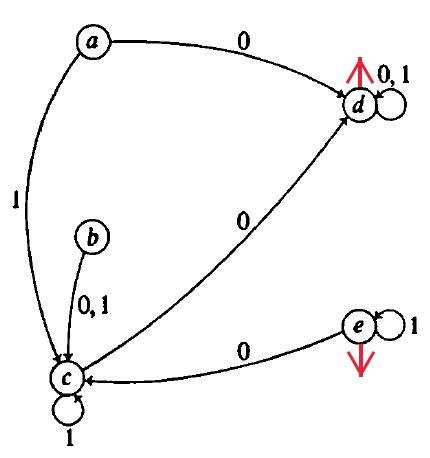
\includegraphics[scale=0.4] {mini-fa} 
	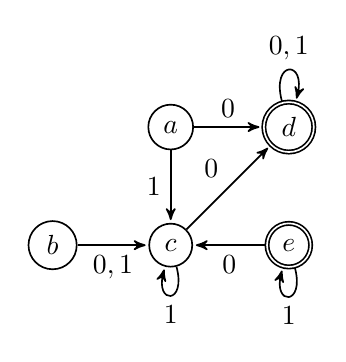
\begin{tikzpicture}[->,>=stealth',shorten >=1pt,auto,node distance=1.5cm, semithick]
	\tikzstyle{every state}=[minimum size=0.1mm]
	\node[state] (a) {$a$};
	\node[state,accepting] (d) [right of=a] {$d$};
	\node[state] (c) [below of=a] {$c$};
	\node[state] (b) [left of=c] {$b$};
	\node[state,accepting] (e) [right of=c] {$e$};
	\path
	(d) edge [loop above] node {$0,1$} (d)
	(c) edge [loop below] node {$1$} (c)
	(e) edge [loop below] node {$1$} (e)
	(a) edge [] node {$0$} (d)
	(a) edge [swap] node {$1$} (c)
	(b) edge [swap] node {$0,1$} (c)
	(e) edge [] node {$0$} (c)
	(c) edge [] node {$0$} (d)
	;
	\end{tikzpicture}
	\caption{Finite state automaton}
	\label{fig:mini-ex2}
\end{figure}

\section{From \cite{Ratnesh95}}

FSM: Finte State Machine

NFSM: Non-deterministic Finite State Machine without $\epsilon-$moves

DFSM: Deterministic Finite State Machine

\begin{definition}[prefix closure of $K$]
	The prefix closure of $K$, denoted $pr(K)\subseteq\Sigma^\ast$, is the language
	\[pr(K):=\{s\in\Sigma^\ast|\exists t\in K:s\le t \}\]
\end{definition}

\begin{example}[Language]\label{ex:language}
	 Consider for example a buffer of capacity one; it has two different states: empty and full. When an \textit{arrival} event occurs in the empty state, then the buffer becomes full; and when a \textit{departure} event occurs in the full state, then the buffer becomes empty. No other state transition can occur in the buffer. Suppose initially the buffer is empty. Then the language of the buffer consists of all possible sequences of the type:
	 $$arrival\cdot departure\cdot arrival\cdot departure \dots,$$
	 where $``\cdot"$ denotes the operation of concatenation.
	 $\hfill\square$
\end{example}

\begin{example}[Generated language]\label{ex:gen_language}
	Consider the buffer of Example \ref{ex:language} Let $a$, $d$ denote the arrival, departure events respectively. Then the generated language of the buffer is $pr((a\cdot d)^\ast)$. Suppose a trace $s\in pr((a\cdot d)^\ast)$ corresponds to completion of a task if and only if its execution results in the empty state of the buffer. Then the marked language of the buffer equals $(a\cdot d)^\ast$.
	$\hfill\square$
\end{example}

\begin{example}[language model]\label{ex:language_model}
	Consider the buffer of Examples \ref{ex:language} and \ref{ex:gen_language} with language	model $[(ad)^\ast,pr((ad)^\ast)]$. The directed graph shown in Figure \ref{fig:DSM} represents a DSM $G:=(X,\Sigma,\alpha,x_0,X_m)$ for the buffer, where $X=\{empty,full\};\Sigma=\{a, d\}; x_0 = empty; X_m = \{empty\};$ and $\alpha(empty, a) = full, \alpha(full, d) = empty$. Note that $\alpha(empty, d)$ and $\alpha(full, a)$ are not defined; hence the transition function is a partial map. (A node in the graph represents a state; a label on a node represents the name of the corresponding state; a directed edge represents a state transition; a label on a directed edge represents the name of the corresponding event; an arrow entering a node represents an initial state; and a circled node represents a marked state.)
	\begin{figure}[htbp]
		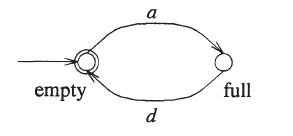
\includegraphics[scale=0.4] {DSM} 
		\caption{Graph representing a DSM}
		\label{fig:DSM}
	\end{figure}
	$\hfill\square$
\end{example}

\begin{example}[Synchronous]
	Consider for example a manufacturing production line consisting
	of a machine (M) and a buffer (B) of capacity one operating in synchrony as shown in Figure \ref{fig:logical-sync}. The event set $\Sigma_1$ of $M$ consists of events $a_1$ representing arrival into the machine, and $d_1$ representing departure from the machine; whereas the event set $\Sigma_2$ of $B$ consists of events $d_1$ representing departure from the machine, and $d_2$ representing departure from buffer. The synchronous composition of two systems is also shown if Figure \ref{fig:logical-sync}.
	\begin{note}
		$d_1$是共享事件,因此,(idle,empty)状态下,$d_1$不能发生, 仅发生 $a_1$事件; (working,empty)状态下,$d_1$在M和B中的转移函数均有定义,因此该共享事件可以发生该共享事件。非共享事件$(a_1,d_2)$在M或B中的转移函数有一个有定义,即可发生。
	\end{note}
	$\hfill\square$
	
	\begin{figure}[htbp]
		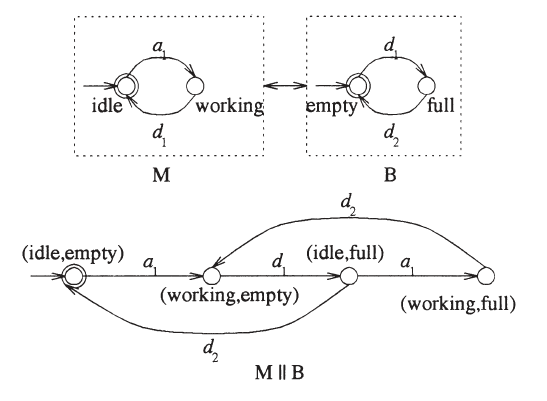
\includegraphics[scale=0.4] {sync} 
		\caption{Diagram illustrating synchronous composition of DFSMs}
		\label{fig:logical-sync}
	\end{figure}
\end{example}

\begin{example}[$\epsilon$-NSM] Consider the $\epsilon$-NSM of Fig. \ref{fig:logical-1model}  Then $\epsilon_G^\ast(1)=\{1,2,3\},\epsilon_G^\ast(2)=\{2,3\},\epsilon_G^\ast(3)=\{3\}.$

so $T(1,\epsilon)=\epsilon_G^\ast(1)=\{1,2,3\}; T(1,a)=\epsilon_G^\ast(T(T(1,\epsilon),a))=\epsilon_G^\ast(T(\{1,2,3\},a)=\epsilon_G^\ast(\{1,3\})=\{1,2,3\}; T(1,ab)=\epsilon_G^\ast(T(\{1,2,3\},b)=\epsilon_G^\ast(\{2\})=\{2,3\}$, etc. $\hfill\square$
	\begin{figure}[htbp]
		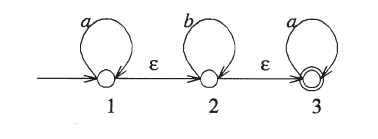
\includegraphics[scale=0.4] {logical-1model} 
		\caption{Diagram illustrating an $\epsilon-NSM$}
		\label{fig:logical-1model}
	\end{figure}
\end{example}


\begin{example}[Completion and reverse]
	Completion and reverse of the DSM of Figure \ref{fig:logical-NFSM-DFSM}(b) are shown
	in Figure \ref{fig:logical-completion-reverse} (a) and \ref{fig:logical-completion-reverse} (b) respectively. The state labels have been changed.
	\begin{figure}[htbp]
		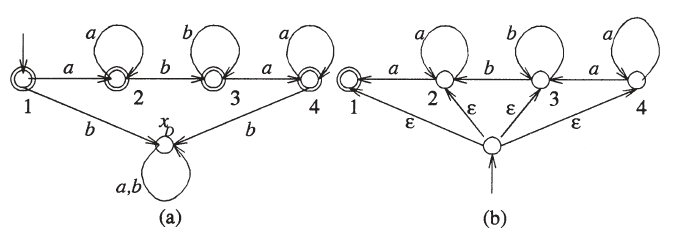
\includegraphics[scale=0.4] {completion-reverse} 
		\caption{Diagram illustrating completion and reverse operations}
		\label{fig:logical-completion-reverse}
	\end{figure}
\end{example}

\begin{theorem}[power set construction]\label{theorem:power_set_cons}
	Let $G:=(X,\Sigma,\alpha,x_0,X_m)$ be a NFSM. Then there exists a language model equivalent DFSM $\mathcal{G}:=(\mathcal{X},\Sigma,\hat{\alpha},\{x_0\},\mathcal{X}_m)$ and $L(\mathcal{G})=L(G)$
\end{theorem}

\begin{proof} Define $\mathcal{X}:=2^X,\mathcal{X}_m:=\{\hat{X}\in\mathcal{X}|\hat{X}\cap X_m\ne \emptyset \}$, and
	\[ \forall \hat{X}\in\mathcal{X},\sigma\in\Sigma:\hat{\alpha}(\hat{X},\sigma):=\bigcup_{x\in\hat{X}}\alpha(x,\sigma) \]
	
	Then is is easily show that $(L_m(\mathcal{G}),L(\mathcal{G}))=(L_m(G),L(G))$
\end{proof}

\begin{example}(NFSM to DFSM)
	Consider the NFSM $G:=(X,\Sigma,\alpha,x_0,X_m)$ shwown in Figure \ref{fig:logical-NFSM-DFSM}(a). The language equivalent DFSM $\mathcal{G}:=(\mathcal{X},\Sigma,\hat{\alpha},\{x_0\},\mathcal{X}_m)$ obtained using the power set construction is shown in Figure \ref{fig:logical-NFSM-DFSM}(b).
	
	Note that $\mathcal{X}=\mathcal{X}_m=\{\{1\},\{1,2,3\},\{2,3\},\{3\} \}$, as $X_m=\{1,3\}$
	
	which has a nonempty intersection with each state in $\mathcal{X}$; 
	\begin{gather*}
	\hat{\alpha}(\{1\},a) = \alpha(1,a) = \{1,2,3\}; \\
	\hat{\alpha}(\{1, 2, 3\}, a) = \alpha(1,a)\cup\alpha(2,a)\cup\alpha(3,a) = \{1, 2, 3\};\\ 
	\hat{\alpha}(\{1, 2, 3\}, b) = \alpha(1, b)\cup\alpha(2, b)\cup\alpha(3, b) = \{2,3\};\\
	etc.
	\end{gather*}

	\begin{figure}[htbp]
		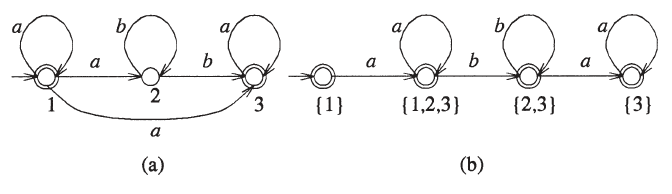
\includegraphics[scale=0.4] {NFSM-DFSM} 
		\caption{Diagram illustrating NFSM to DFSM conversion}
		\label{fig:logical-NFSM-DFSM}
	\end{figure}
\end{example}

\begin{remark}
	It follows from Theorems \ref{theorem:power_set_cons} that if a language model $(K_m, K)$ can be represented as a finite state machine $G$, then there also exists a DFSM $G^\prime$ such that $(L_m(G^\prime), L(G^\prime)) = (K_m, K)$. Thus if we are only concerned with DESs that have finitely many states, then we can assume without loss of generality that they can be represented as DFSMs. We will see below that although the finiteness of states is not needed for most of the analysis, it is needed for developing all the decision algorithms.
	
	However, it should be noted that although DFSMs are useful in developing decision algorithms, it is conceptually easier to obtain a NFSM from the given description of a language. For example, suppose $\Sigma = \{a,b\}$, and suppose we	wish to represent the language with the property that every string in it must contain $aba$ as a substring. A NFSM for the same is shown in Figure \ref{fig:NFSM-DFSM1}(a); corresponding DFSM obtained using the construction outlined in Theorem \ref{theorem:power_set_cons}
	is shown in Figure \ref{fig:NFSM-DFSM1}(b).
\end{remark}

\begin{figure}[htbp]
	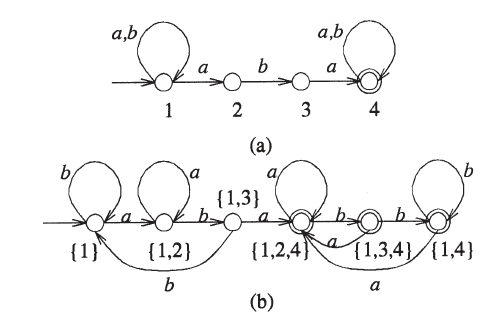
\includegraphics[scale=0.4] {NFSM-DFSM1} 
	\caption{NFSM accepting strings with aba as a substring, and corresponding DFSM}
	\label{fig:NFSM-DFSM1}
\end{figure}

\subsection{Myhill-Nerode Characterization}

\begin{definition}[equivalence relation$(R_K)$]
	Given a language $K\subseteq \Sigma^\ast$, it induces an equivalence relation, denoted $R_K$, on $\Sigma^\ast$:
	\[ \forall s,t\in\Sigma^\ast: s\cong t(R_K)\Leftrightarrow [K\setminus\{s\}=K\setminus\{t\}] \]
	For each $s\in\Sigma^\ast,[s]R_K\subseteq\Sigma^\ast$ is used to denote the equivalence class containing the string $s$.
\end{definition}

\begin{definition}[equivalence relation$(R_G)$]
	Given a DFSM $G:=(X,\Sigma,\alpha,x_0,X_m)$, it induces an equivalence relation, denoted $R_G$, on $\Sigma^\ast$:
	\[ \forall s,t\in\Sigma^\ast: s\cong t(R_G)\Leftrightarrow [\alpha(x_0,s)=\alpha(x_0,t)]\lor[\alpha(x_0,s)=\alpha(x_0,t) \text{ undefined}] \]
	For each $s\in\Sigma^\ast,[s]R_G\subseteq\Sigma^\ast$ is used to denote the equivalence class containing the string $s$.
\end{definition}

\begin{note}
	Note the $R_G$, the \textit{index} of $R_G$, i.e., the number of equivalence classes of $R_G$, is one more than the number of states in $G$, $|R_G|=|G|+1$. (The set of all strings that do not
	belong to $L(G)$ belong to a single equivalence class of $R_G$.) 
\end{note}

It can be easily seen that the equivalence relation $R_G$ refines the equivalence relations $R_{L_m(G)}$ and $R_{L(G)}$. In other words,
\[ \forall s,t\in\Sigma^\ast : s\cong t(R_G)\Rightarrow [s\cong t(R_{L_m(G)})]\land [s\cong t(R_{L(G)})] \]

An equivalence relation $R$ on $\Sigma^\ast$ is said to be \textit{right invariant (with respect to concatenation)} if
\[ \forall s,t\in\Sigma^\ast : s\cong t(R) \Rightarrow su\cong tu(R) \]

It is easy to verify that $R_K$ as well as $R_G$ defined above are right invariant.The following proposition is due to Myhill and Nerode:

\begin{theorem}[Myhill and Nerode]\label{theorem:MyhillNerode}
	Let $K\subseteq\Sigma^\ast$ be a language. Then the following are equivalent:
	\begin{enumerate}[1. ]
		\item $K$ is regular.
		\item $K$ can be written as union of some of the equivalence classes of a right invariant equivalence relation of finite index.
		\item $R_K$ is of finite index.
	\end{enumerate}
\end{theorem}

\begin{proof}
	$(1)\Rightarrow (2)$: Suppose $K$ is regular. Then there exists a DFSM $G$ such that $L_m(G) = K$. Then clearly $K$ can be written as union of the following equivalence classes of $R_G$:
	\[\{[s](R_G)|s\in K \}\]
	
	This proves the first assertion implies the second assertion, as $R_G$ is right invariant.
	
	$(2)\Rightarrow (3)$: Let R be a right invariant equivalence relation of finite index such that $K$ can be written as union of some of the equivalence classes of $R$. In order to show that $R_K$ is of finite index it suffices to show that $R$ refines $R_K$. Pick $s,t\in\Sigma^\ast$  such that $s\cong t(R)$. Since $R$ is right invariant, for any $u\in\Sigma^\ast,su\cong tu(R)$. Since $K$ equals union of some of the equivalence classes of $R$, this implies $su\in K$ if and only if $tu\in K$. In other words, $s\cong t(R_K)$, which proves that the second assertion implies the third assertion.
	
	$(3)\Rightarrow (1)$: Finally, suppose $R_K$ is of finite index. Define a DFSM $G:=(\hat{X},\Sigma,\hat{\alpha},\hat{x}_0,\hat{X}_m)$ as follows: $\hat{X}:=\{[s](R_K)|s\in\Sigma^\ast\}; x_0 :=[\epsilon](R_K); \hat{X}_m=\{[s](R_K)|s\in K \}$;
	and
	\[ \forall [s](R_k)\in\hat{X},\sigma\in\Sigma:\hat{\alpha}([s](R_K),\sigma):=[s\sigma](R_K) \]
	
	Then it is readily verified that for each $s\in\Sigma^\ast,\hat{\alpha}(\hat{x}_0,s)=[s](R_K)$. Hence
	from definition of marked language we obtain that $s\in L_m(G)$ if and only if $\hat{\alpha}(\hat{x}_0,s) = [s](R_K) \in X_m$, i.e., if and only if $s\in K$. Thus $L_m(G) = K$. Since $\hat{G}$ is a DFSM (as $R_K$ is of finite index), this implies that $K$ is regular; so the third assertion implies the first assertion. $\hfill\square$
\end{proof}

The construction of the DFSM G in the proof of Theorem \ref{theorem:MyhillNerode} is known as the Myhill-Nerode construction. The following example illustrates such a construction.

\begin{example}[equivalence classes]
	Consider for example the marked language $K_m = (ad)^\ast$ of
	the buffer of capacity one of Example \ref{ex:gen_language}. 
	Then the generated language of the buffer is $pr((a\cdot d)^\ast)=pr(K_m)$. Suppose a trace $s\in pr((a\cdot d)^\ast)$ corresponds to completion of a task if and only if its execution results in the empty state of the buffer. Then the marked language of the buffer equals $(a\cdot d)^\ast$.
	
	Clearly, $K_m$ is a regular language.
	Hence it follows from Theorem \ref{theorem:MyhillNerode} that $R_{K_m}$ is of finite index. It can be easily verified that
	\begin{gather*}
		[\epsilon](R_{K_m})=(ad)^\ast=K_m\\
		[a](R_{K_m})=(ad)^\ast a=pr(K_m)-K_m\\
		[d](R_{K_m})=\{a,d\}^\ast-pr(K_m)
	\end{gather*}
	and these are the only equivalence classes of $R_{K_m}$
	
	Hence Myhill-Nerode construction yields the DFSM $G:=(\hat{X},\Sigma,\hat{\alpha},\hat{x}_0,\hat{X}_m)$, while\\ 
	$\hat{X}=\{[\epsilon](R_{K_m}),[a](R_{K_m}),[d](R_{K_m}) \}$;
	$\hat{x}_0=[\epsilon](R_{K_m}); X_m=\{[\epsilon](R_{K_m}) \}$;\\
	and
	\begin{align*}
		\hat{\alpha}([\epsilon](R_{K_m}),a)&=[a](R_{K_m});\\
		\hat{\alpha}([\epsilon](R_{K_m}),d)&=[d](R_{K_m});\\
		\hat{\alpha}([a](R_{K_m}),a)&=[aa](R_{K_m})=[d](R_{K_m});\\
		\hat{\alpha}([a](R_{K_m}),d)&=[ad](R_{K_m})=[\epsilon](R_{K_m});\\
		\hat{\alpha}([d](R_{K_m}),a)&=[da](R_{K_m})=[d](R_{K_m});\\
		\hat{\alpha}([d](R_{K_m}),d)&=[dd](R_{K_m})=[d](R_{K_m});
	\end{align*}
	
	See figure \ref{fig:equiv}, State e: empty,$[\epsilon](R_{K_m})$;
	State f: full,$[a](R_{K_m})$;  State t: dump/trap,$[d](R_{K_m})$.
	
	\begin{figure}[htbp]
      \centering
	  \subfigure[buffer model]
	  {
	  	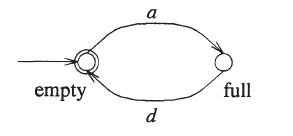
\includegraphics[scale=0.4] {DSM}
	  }
      \hspace{2cm} % 如果并列,用\\换行即可
      \subfigure[equivalence classes]
      {
		  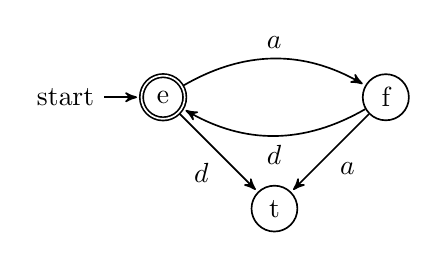
\begin{tikzpicture}[->,>=stealth',shorten >=1pt,auto,node distance=2cm, semithick]
		  \tikzstyle{every state}=[minimum size=0.1mm]
		  \node[state]         (t) {t};
		  \node[initial,state,accepting] (e) [above left of=t] {e};
		  \node[state]         (f) [above right of=t] {f};
		  \path
		  (e) edge [bend left]  node {$a$} (f)
		      edge [swap] node {$d$} (t)
		  (f) edge [bend left]  node {$d$} (e)
		      edge [] node {$a$} (t)
		  ;
		  \end{tikzpicture}
		  (states e:empty,f:full,t:dump/trap) 
      }
	  \caption{equivalence classes}
	  \label{fig:equiv}
	\end{figure}
	$\hfill\square$
\end{example}

\begin{remark}
	Given a regular language K, there always exists a DFSM $G$ such
	that $L_m(G) = K$. Hence there exists a minimal such DFSM (one with a minimal number of states). Let $G^\prime$ be the DFSM obtained by removing the state $[s](R_K)$ form $\hat{G}$ (and all transitions leading into/out of it), where $\hat{G}$ is the DFSM in the proof of Theorem \ref{theorem:MyhillNerode} and $s\in \Sigma^\ast$ is such that $s\notin pr(K)$.Then it is easy to see that $L_m(G^\prime) = K$. In fact $G^\prime$ is a minimal DFSM with marked language $K$. In order to see this first note that the number of states in $\hat{G}$ is $|R_K|$, the index of $R_K$. Since $G^\prime$ is obtained by removing a single state from $\hat{G}$, the number of states in $G^\prime$ equals $|R_K|-1$. Let $G$ be any DFSM with $L_m(G) = K$. Then as noted above number of states in $G$ equals $|R_G|-1$. Also,as noted above, $R_G$ refines $R_{L_m(G)} = R_K$, which implies that $|R_K|\le |R_G|$. Thus $|R_K| - 1\le |R_G| - 1$, which proves that $G^\prime$ is a minimal DFSM with marked language $K$.
\end{remark}

\subsection{Minimization}

\begin{theorem}[Minimal $K$] \label{theorem:Minimal}
	Suppose $K\subseteq \Sigma^\ast$ is a regular language. Then a trim DFSM $G:=(X,\Sigma,\alpha,x_0,X_m)$ with marked language $K$ is mininmal if and only if
	$$\forall x,x^\prime\in X,s\in \Sigma^\ast :(\alpha(x,s),\alpha(x^\prime,s))\in X_m\times X_m\Rightarrow x=x^\prime .$$
\end{theorem}

Suppose $K\subseteq \Sigma^\ast$ is regular. Let $G:=(X,\Sigma,\alpha,x_0,X_m)$ be a trim DSFSM such that $L_m(G)=K$. We are interested in obtaining a minimal DFSM with marked language $K$ by combining some of the ``language equivalent" states of $G$. Note that if $K = \Sigma^\ast$, then it can be accepted by a minimal DFSM having a single state. Hence we assume without loss of generality that $K\ne\Sigma^\ast$.

DFSM $G:=(X,\Sigma,\alpha,x_0,X_m)$ induces an equivalence relation on $X$ defined as:
\[ \forall x,x^\prime\in X:x\cong x^\prime \Leftrightarrow [\forall s\in\Sigma^\ast:\alpha(x,s)\in X_m\Leftrightarrow\alpha(x^\prime,s)\in X_m] \]

Using this equivalence relation we define a language equivalent DFSM $\hat{G}:=(\hat{X},\Sigma,\hat{\alpha},\hat{x}_0,\hat{X}_m)$, where $\hat{X}:=\{[x]|x\in X\},\hat{x}_0:=[x_0],\hat{X}_m:=\{[x]|x\in X_m\}$, and
\[
\forall [x]\in\hat{X},\sigma\in\Sigma:\hat{\alpha}([x],\sigma):=\left\{ 
\begin{aligned}
\left[\alpha(x,\sigma)\right]  &\text{   if $\alpha(x,\sigma)$ defined}\\ 
\text{undefined} &\text{    otherwise}\\
\end{aligned} 
\right. 
\]

Using the fact that $G$ is trim, it is readily verified that $\hat{G}$ is well defined, and $(L_m(\hat{G}),L(\hat{G}))=(L_m(G),L(G))=(K,pr(K))$. Moreover, it follows from Theorem \ref{theorem:Minimal} that $\hat{G}$ is a minimal state machine with marked language $K$.

An algorithm for efficiently identifying the equivalence classes $\{[x]|x\in X\}$ is presented next. Note that each state pair $(x,x^\prime)\in (X_m\times X_m)\cup [(X-X_m)\times (X-X_m)]$ is a possible pair of equivalent states. 

First consider $\bar{G}:=(\bar{X},\Sigma,\bar{\alpha},x_0,X_m)$, the completion of $G$. Then since $K\ne\Sigma^\ast,X_m\ne\bar{X}=X\cup\{x_D\}$, while $X_D$ is the ``dump" state. This implies $\bar{X}-X_m\ne\emptyset$.

\begin{note}
	Note that if $K = \Sigma^\ast$, then it can be accepted by a minimal DFSM having a single state.
\end{note}

\begin{figure}[htbp]
	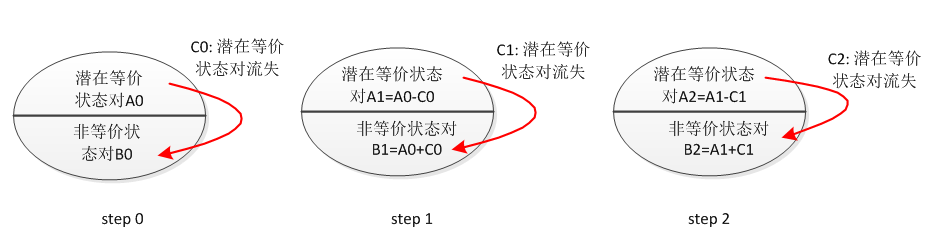
\includegraphics[scale=0.4] {algo-minimize} 
	\caption{Diagram illustrating algorithm minimize}
	\label{fig:algo-minimize}
\end{figure}

\begin{algorithm}  
	\caption{The algorithm for a minimal DFSM, see Figure \ref{fig:algo-minimize}}  
	\begin{algorithmic}[1] %每行显示行号  
		\Require $G=(\bar{X},\Sigma,\alpha,\_,X_m)$  
		\Ensure The equivalence classes of $X$ 
		
		A: \{潜在等价状态对\}; B: \{非等价状态对\}; C: \{本次迭代流失的潜等价状态对\}
		
		\State Initiation step:
		
		$A_0 := [X_m\times X_m]\cup [(\bar{X}-X_m)\times(\bar{X}-X_m)]=\{\text{(final状态对)}\cup \text{(非final状态对)} \} = \{\text{潜在的等价状态对}\}$; 
		
		$B_0 := [\bar{X}\times\bar{X}-A_0] = \{\text{(全体状态对)}-A_0 \} = \{\text{(final状态,非final状态)} \} = \{\text{非等价状态对}\} = \{\text{非$A_0$状态对}\}$; 
		
		$k:=0$.
		
		\State Iteration step:
		\begin{align*}
			C_k &:= \{(x,x^\prime)\in A_k | \exists\sigma\in\Sigma \text{ s.t. } (\alpha(x,\sigma),\alpha(x^\prime,\sigma))\in B_k \} \\
			&=\{\text{$A_0$中两大类中的(状态对)存在字母$\sigma$进入$B_0$类)} \} \\
			&= \{ \text{潜在状态对 $\to$ 非等价状态对} \}\\
			A_{k+1} &:= A_k - C_k \\
			B_{k+1} &:= B_k\cup C_k =[\bar{X}\times \bar{X}] - A_{k+1}\\
			&=\{\text{非$A_{k+1}$状态对}\}
		\end{align*}
		
		\State Termination step:
		
		if $A_{k+1}=A_k$, then stop; else, $k := k+1$, and goto step 2.
	\end{algorithmic}
    \label{alg:minimal}   
\end{algorithm}

It can be verified that after termination, each state pair in $A_k$ is an equivalent pair of states. Finally, the minimal state machine $G$ is obtained by combining each state pair in $A_k$ as described above, and removing the equivalence class of the dump state.

Algorithm \ref{alg:minimal} terminates in $O(m^2)$ steps, where $m$ is the number of states in $G$.

\begin{example}
	Consider the complete DFSM of Figure \ref{fig:complete}. Then $X_m=\{1,2,3,4 \}$ and $X=\{1,2,3,4,x_D \}$. Algorithm \ref{alg:minimal} can be  applied to minimize the DFSM as follows:
	\begin{align*}
		A_0 &=[X_m\times X_m]\cup\{(x_D\times x_D)\};\\
		&=\{(1,1),(2,2),(3,3),(4,4),(1,2),(2,1),(1,3),(3,1),(1,4),(4,1),(2,3),(3,2),(2,4),(4,2),(3,4),(4,3) \} \cup\{(x_D,x_D) \}\\
		&=\{(1,1),(2,2),(3,3),(4,4) \}\cup\{(1,2),(1,3),(1,4),(2,3),(2,4),(3,4) \}\cup
		\{(2,1),(3,1),(4,1),(3,2),(4,2),(4,3)\}\cup\{x_D,x_D\}\\
		&= \{\text{潜在的等价状态对}\} \\
		B_0 &=[X\times X]-A_0\\
		&=\{(1,x_D),(x_D,1),(2,x_D),(x_D,2),(3,x_D),(x_D,3),(4,x_D),(x_D,4) \}\\
		&=\{(1,x_D),(2,x_D),(3,x_D),(4,x_D) \} \cup \{(x_D,1),(x_D,2),(x_D,3),(x_D,4) \}\\
		&= \{\text{非等价状态对}\} = \{\text{非$A_0$状态对}\}\\
		C_0 &= \{(1,2),(2,1),(1,3),(3,1),(2,4),(4,2),(3,4),(4,3)\}\\
		&=\{(1,2),(1,3),(2,4),(3,4) \}\cup\{(2,1),(3,1),(4,2),(4,3) \}\\
		&= \{ \text{潜在状态对$(A_0) \to (B_0)$非等价状态对} \}\\
		A_1 &= A_0-C_0\\
		&=\{(1,1),(2,2),(3,3),(4,4) \}\cup\{(1,4),(2,3) \}\cup
		\{(4,1),(3,2) \}\cup\{x_D,x_D\}\\
		B_1 &= [X\times X]-A_1\\
		&= \{\text{非$A_1$状态对}\}\\
		C_1 &= \{ \text{潜在状态对($A_1) \to (B_1)$非等价状态对} \}\\
		&= \{(1,4),(4,1),(2,3),(3,2)\}\\
		A_2 &= A_1-C_1\\
		&= \{(1,1),(2,2),(3,3),(4,4),(x_D,x_D)\}\\
		B_2 &=[X\times X] - A_2
	\end{align*}
    Clearly, all the state pairs in $A_2$ are equivalent pairs, i.e. $C_2 = \emptyset$: hence the algorithm terminates. Thus the minimal DFSM is the DFSM of Figure \ref{fig:complete}, which does not contain the dump state.
	\begin{figure}[htbp]
		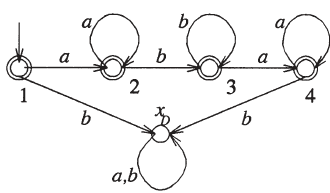
\includegraphics[scale=0.4] {complete} 
		\caption{the minimal DFSM is not contain the dump state}
		\label{fig:complete}
	\end{figure}
\end{example}

\section{From wiki -- Partition of a set}

From \url{https://en.wikipedia.org/wiki/Partition_of_a_set}.

\begin{definition}[a partition of a set] 
	A partition of a set $X$ is a set of nonempty subsets of $X$ such that every element $x$ in $X$ is in exactly one of these subsets (i.e., $X$ is a disjoint union of the subsets).
	Equivalently, a family of sets $P$ is a partition of $X$ if and only if all of the following conditions hold:
	\begin{itemize}
		\item The family $P$ does not contain the empty set (that is $\emptyset \notin P)$.
		\item The union of the sets in $P$ is equal to $X$ (that is $\bigcup _{A\in P}A = X)$ . The sets in $P$ are said to \textbf{cover} $X$.
		\item The intersection of any two distinct sets in $P$ is empty (that is $(\forall A,B\in P)\;A\neq B\implies A\cap B=\emptyset)$. The elements of $P$ are said to be pairwise disjoint.
	\end{itemize}
	
	The sets in P are called the \textit{blocks, parts} or \textit{cells} of the partition.
	
	The rank of $P$ is $|X| − |P|$, if $X$ is finite.
\end{definition}

\begin{example}[a partition of a set]
	(From \url{https://en.wikipedia.org/wiki/Partition_of_a_set})
	\begin{itemize}
		\item The empty set $\emptyset$ has exactly one partition,namely $\emptyset$.
		\item For any nonempty set $X, P = \{X\}$ is a partition of $X$, called the trivial partition.
		\subitem Particularly, every singleton set $\{x\}$ has exactly one partition, namely $\{ \{x\} \}$.
		\item For any non-empty proper subset $A$ of a set $U$, the set $A$ together with its complement form a partition of $U$, namely, $\{A, U \setminus A \}$.
		\item The set $\{ 1, 2, 3 \}$ has these five partitions (one partition per item):
		\begin{itemize}
			\item $\{ \{1\}, \{2\}, \{3\} \}$, sometimes written $1|2|3$.
			\item $\{ \{1, 2\}, \{3\} \}$, or $12|3$.
			\item $\{ \{1, 3\}, \{2\} \}$, or $13|2$.
			\item $\{ \{1\}, \{2, 3\} \}$, or $1|23$.
			\item $\{ \{1, 2, 3\} \}$, or $123$ (in contexts where there will be no confusion with the number).
		\end{itemize}
		\item The following are not partitions of $\{ 1, 2, 3 \}$:
		\begin{itemize}
			\item \{ \{\}, \{1, 3\}, \{2\} \} is not a partition (of any set) because one of its elements is the empty set.
			\item $\{ \{1, 2\}, \{2, 3\} \}$ is not a partition (of any set) because the element $2$ is contained in more than one block.
			\item $\{ \{1\}, \{2\} \}$ is not a partition of $\{1, 2, 3\}$ because none of its blocks contains $3$; however, it is a partition of $\{1, 2\}$.
		\end{itemize}
	\end{itemize}
\end{example}

\begin{definition}[Partitions and equivalence relations]
	For any equivalence relation on a set $X$, the set of its equivalence classes is a partition of $X$. Conversely, from any partition $P$ of $X$, we can define an equivalence relation on $X$ by setting $x\equiv y$ precisely when $x$ and $y$ are in the same part in $P$. Thus the notions of equivalence relation and partition are essentially equivalent.
	
	The axiom of choice guarantees for any partition of a set $X$ the existence of a subset of $X$ containing exactly one element from each part of the partition. This implies that given an equivalence relation on a set one can select a canonical representative element from every equivalence class.
\end{definition}

\begin{definition}[Refinement of partitions]
	A partition $\alpha$ of a set $X$ is a refinement of a partition $\rho$ of $X$—and we say that $\alpha$ is finer than $\rho$ and that $\rho$ is coarser than $\alpha$—if every element of $\alpha$ is a subset of some element of $\rho$. Informally, this means that $\alpha$ is a further fragmentation of $\rho$. In that case, it is written that $\alpha\le\rho$.
	
	This finer-than relation on the set of partitions of $X$ is a partial order (so the notation $``\le"$ is appropriate). Each set of elements has a least upper bound and a greatest lower bound, so that it forms a lattice, and more specifically (for partitions of a finite set) it is a geometric lattice. The partition lattice of a 4-element set has 15 elements and is depicted in the Hasse diagram on the Fig \ref{fig:Hasse}.
	
	Based on the cryptomorphism between geometric lattices and matroids, this lattice of partitions of a finite set corresponds to a matroid in which the base set of the matroid consists of the atoms of the lattice, namely, the partitions with $n-2$ singleton sets and one two-element set. These atomic partitions correspond one-for-one with the edges of a complete graph. The matroid closure of a set of atomic partitions is the finest common coarsening of them all; in graph-theoretic terms, it is the partition of the vertices of the complete graph into the connected components of the subgraph formed by the given set of edges. In this way, the lattice of partitions corresponds to the lattice of flats of the graphic matroid of the complete graph.
	
	Another example illustrates the refining of partitions from the perspective of equivalence relations. If D is the set of cards in a standard 52-card deck, the same-color-as relation on D – which can be denoted ~C – has two equivalence classes: the sets {red cards} and {black cards}. The 2-part partition corresponding to ~C has a refinement that yields the same-suit-as relation ~S, which has the four equivalence classes {spades}, {diamonds}, {hearts}, and {clubs}.
	
	\begin{figure}[htbp]
		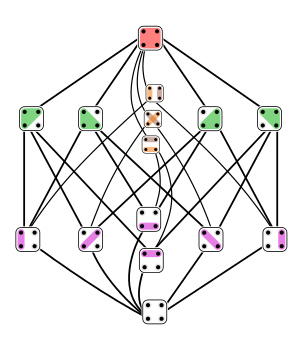
\includegraphics[scale=0.8]{Hasse.png}
		\caption{Partitions of a 4-set ordered by refinement}
		\label{fig:Hasse}
	\end{figure}
\end{definition}

\section{From \cite{Kenneth2012}}

\begin{definition}[等价关系]
	定义在集合$A$上的关系叫做等价关系,如果它是自反的、对称的和传递的。
\end{definition}

\begin{definition}[等价元素]
	如果两个元素$a$和$b$由于等价关系而相关联,则称它们是等价的。记法$a\sim b$通常用来表示对于某个特定的等价关系来说,$a$和$b$是等价的元素。
\end{definition}

\begin{note}
	在等价关系中,若两个元素有关系,就可以说它们是等价的。为了使等价元素的概念有意义,每个元素都应该等价于它自身,因为对于等价关系来说,自反性是一定成立的。在等价关系中,说$a$和$b$是相互关联也是正确的(而不仅是$a$关联于$b$),因为如果$a$关联于$b$, 右对称性, $b$也关联于$a$。
	
	此外,因为等价关系是传递的,所以如果$a$和$b$等价且$b$和$c$等价,则可得出$a$和$c$也是等价的。
\end{note}

\begin{example}
	设$R$是定义在整数集上的关系,满足$aRb$当且仅当$a=b$或$a=-b$。可以证明$R$是自反的,对称的和传递的。因此$R$是等价关系。
\end{example}

\begin{example}[模$m$同余]
	设$m$是大于1的整数。证明以下关系是定义在整数集上的等价关系。
	\[R=\{(a,b)|a\equiv b\pmod{m}\} \]
\end{example}

\begin{proof}
	$a\equiv b\pmod{m}$, 当且仅当$m$整除$a-b$。 注意$a-a=0$能被$m$整除,因为$0=0\cdot m$。因此$a\equiv a\pmod{m}$, 从而模$m$同余关系是自反的。
	
	假设$a\equiv b\pmod{m}$, 那么$a-b$能被$m$整除,即$a-b=km$, 其中$k$是整数。从而$b-a=(-k)m$, 即$b\equiv a\pmod{m}$, 因此模$m$同余关系是对称的。
	
	下面假设$a\equiv b\pmod{m}$和$b\equiv c\pmod{m}$, 那么$m$整除$a-b$和$b-c$。因此存在整数$k$和$l$, 使得$a-b=km$和$b-c=lm$, $\implies a-c=(a-b)+(b-c)=km+lm=(k+l)m$。于是$a\equiv c\pmod{m}$, 从而模$m$同余关系是传递的。
	
	综上所述,模$m$同余关系是等价的。
\end{proof}

\begin{example}
	设$R$是定义在英文字母组成的字符串的集合上的关系,满足$aRb$当且仅当$l(a)=l(b)$, 其中$l(x)$是字符串$x$的长度。证明$R$是等价关系。
\end{example}

\begin{proof}
	因为$l(a)=l(a)$, 所以只要$a$是一个字符串,就有$aRa$, 故$R$是自反的。其次,假设$aRb$, 即$l(a)=l(b)$, 那么有$bRa$, 因为$l(b)=l(a)$, 所以$R$是对称的。最后,假设$aRb$且$bRc$, 那么有$l(a)=l(b),l(b)=l(c)\implies l(a)=l(c)$, 即$aRc$, 从而$R$是传递的。由于$R$是自反的,对称的和传递的,所以$R$是等价关系。
\end{proof}

\begin{example}\label{ex:eqstr}
	设$n$是正整数,$S$是字符串集合。假定$R_n$是$S$上的关系,$sR_n t$当且仅当$s=t$或者$s$和$t$都至少含有$n$个字符,且$s$和$t$的前$n$个字符相同。就是说,少于$n$个字符的字符串只于它自身的$R_n$相关;一个至少含有$n$个字符的字符串$s$与字符串$t$相关当且仅当$t$也含有至少$n$个字符且$t$以$s$最前面的$n$个字符开始。例如,设$n=3$, $S$是所有位串的集合,$sR_3t$当$s=t$或者$s$和$t$均为长度至少为3的位串,且前3位相同。例如,$01R_3 01$, $00111R_3 001101$,但是$(01,010)\notin R_3, (0101,01110)\notin R_3$
	
	证明:对所有的字符串集$S$和所有的正整数$n$, $R_n$是定义在$S$上的等价关系。
\end{example}

\begin{proof}
	
	设$s$是$S$中的一个字符串,由于$s=s$, 可得$sR_ns$, 所以$R_n$关系是自反的。
	
	如果$sR_nt$, 那么或者$s=t$或者$s$和$t$都至少含有$n$个字符,且以相同的$n$个字符开始。这意味着$tR_ns$成立。所以$R_n$是对称的。
	
	现在假设$sR_nt$且$tR_nu$。 则有$s=t$或者$s$和$t$都至少含有$n$个字符,且以相同的$n$个字符开始。还有$t=u$或者$t$和$u$都至少含有$n$个字符,且以相同的$n$个字符开始。 由此可以推出$s=u$或者$s$和$u$都至少含有$n$个字符,且以相同的$n$个字符开始(因为在这种情形下,我们知道$s,t$和$u$都至少含有$n$个字符,且$s$和$u$都与$t$一样以相同的$n$个字符开始)。所以$R_n$是传递的。
	
	综上所述,模$R_n$是一个等价关系。
\end{proof}

\begin{definition}[等价类]
	设$R$是定义在集合$A$上的等价关系。与$A$中的一个元素$a$有关系的所有元素的集合叫做$a$的等价类。$A$的关于$R$的等价类记作$[a]_R$。当只考虑一个关系时,我们将省去下标$R$并把这个等价类写作$[a]$。
	
	换句话说,如果$R$是定义在集合$A$上的等价关系,则元素$a$的等价类是
	\[ [a]_R = \{s|(a,s)\in R \}\]
	如果$b\in [a]_R,b$叫做这个等价类的\textbf{代表元}。一个等价类的任何元素都可以作为这个类的代表元。也就是说,选择特定元素作为一个类的代表元没有特殊要求。 
\end{definition}

\begin{example}
	设$R$是定义在整数集上的关系,满足$aRb$当且仅当$a=b$或$a=-b$。可以证明$R$是自反的,对称的和传递的。因此$R$是等价关系。
	
	在这个等价关系中,一个整数对应于它自身和它的相反数数。从而一个整数的等价类是:$[a]=\{a,-a\}$。这个集合包含两个不同的整数,除非$a=0$。例如, $[7]=\{7,-7\},[-5]=\{-5,5\},[0]=\{0\}$。
\end{example}

\begin{example}
	对于模$4$同余关系,0和1的等价类是什么?
	
	0的等价类包含使得$a\equiv 0\pmod{4}$的所有整数$a$。这个类中的整数是能被4整除的那些整数。因此,对于这个关系,0的等价类是
	\[ [0]=\{\cdots,-8,-4,0,4,8,\cdots \}\]
	1的等价类包含使得$a\equiv 1\pmod{4}$的所有整数$a$。这个类中的整数是当被4除时余数为1的那些整数。因此,对于这个关系,1的等价类是
	\[ [1]=\{\cdots,-7,-3,1,5,9,\cdots \}\]
	
	用正整数$m$代替4, 很容易推广到模m同余关系的等价类--模m的同余类。整数$a$模$m$的同余类记作$[a]_m$, 满足
	\[ [a]_m=\{\cdots,a-2m,a-m,a,a+m,a+2m,\cdots \}\] 
	例如,
	\begin{align*}
		[0]_4 &=\{\cdots,-8,-4,0,4,8,\cdots \} \\
		[1]_4 &=\{\cdots,-7,-3,1,5,9,\cdots \} 
	\end{align*}
		
\end{example}

\begin{example}
	对于例\ref{ex:eqstr}中所有位串集合上的等价关系$R_3$, 串$0111$的等价类是什么?
	等价于$0111$的是以$011$开始,至少含有3位的位串:
	\[[011]_{R_3}=\{011,0110,0111,01100,01101,0111111,\cdots\}\]
\end{example}

\begin{theorem} \label{theorem:eqPro}
	设$R$是定义在集合$A$上的等价关系,下面的关于集合$A$中$a,b$两个元素的命题是等价的。
	\begin{enumerate}[(i) ]
		\item $aRb$
		\item $[a]=[b]$
		\item $[a]\cap [b]\ne\emptyset$
	\end{enumerate}
\end{theorem}

\begin{proof}
	首先证明(i)推出(ii)。
	
	假设$aRb$,我们将通过$[a]\subseteq [b]$和$[b]\supseteq [a]$来证明$[a]=[b]$。
	
	假设$c\in [a]$, 那么$aRc$。因为$aRb$是对称的,所以$bRa$。又由于$R$是传递的以及$bRa$和$aRc$, 就得到$bRc$, 所以$c\in [b]$。这就证明了$[a]\subseteq [b]$。 类似地,可证明$[a]\supseteq [b]$。
	
	其次我们将证明(ii)推出(iii)。假设$[a]=[b]$, 这就证明了$[a]\cap [b]\ne\emptyset$, 因为$[a]$是非空的(由$R$的自反性$a\in [a]$)。
	
	下面证明(iii)推出(i)。假设$[a]\cap [b]\ne\emptyset$, 那么存在元素$c$满足$c\in [a]$且$c\in [b]$。换句话说, $aRc$且$bRc$。由对称性, 有$cRb$。再根据传递性,由$aRc$和$cRb$,就有$aRb$。
	
	因为$(i)\implies (ii),(ii)\implies (iii),(iii)\implies (i)$, 所以三个命题是等价的。
\end{proof}

现在我们将说明一个等价关系怎样划分一个集合。设$R$是定义在集合$A$上的的等价关系,$R$的所有等价类的并集就是集合$A$, 因为$A$的每个元素$a$都在它自己的等价类,即$[a]_R$中。换句话说,
\[ \bigcup_{a\in A}[a]_R = A \]
此外,有定理\ref{theorem:eqPro},这些等价类或者是相等的或者是不相交的的,因此当$[a]_R\ne[b]_R$时,
\[ [a]_R\cap [b]_R = \emptyset\]

这两个结论证明了等价类构成$A$的划分, 因为它们将$A$分成不相交的子集。更确切的说,集合$S$的\textbf{划分}是$S$的不相交的非空的子集构成的集合,且它们的并集就是$S$。换句话说,一簇子集$A_i,i\in I$, (其中$I$是下标的集合)构成$S$的划分,当且仅当
\begin{align*}
A_i &\ne \emptyset  &i\in I \\
A_i\cap A_j &=\emptyset  &i\ne j\\
\bigcup_{i\in I}A_i &= S  &
\end{align*}

\begin{figure}[htbp]
	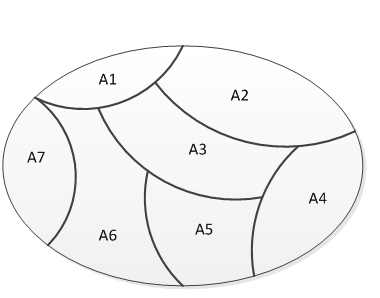
\includegraphics[scale=.4]{partition}
	\caption{Partition of set}
	\label{fig:partition}
\end{figure}

\begin{example}
	假设$S=\{1,2,3,4,5,6\}$, 一簇集合$A_1=\{1,2,3\},A_2=\{4,5\},A_3=\{6\}$构成$S$的一个划分,因为这些集合是不相交的,且它们的并集是$S$。
\end{example}

\begin{theorem}
	设$R$是定义在集合$S$上的等价关系。那么$R$的等价类构成$S$的划分。反过来,给定集合$S$的划分$\{A_i|i\in I\}$, 则存在一个等价关系$R$,它以集合$A_i(i\in I)$作为它的等价类。
\end{theorem}

\begin{example}
	假设$S=\{1,2,3,4,5,6\}$, 一簇集合$A_1=\{1,2,3\},A_2=\{4,5\},A_3=\{6\}$构成$S$的一个划分,因为这些集合是不相交的,且它们的并集是$S$。
	列出这个划分所产生的等价关系$R$中的有序对。
\end{example}

\begin{solution}
	划分中的子集是$R$的等价类。有序对$(a,b)\in R$, 当且仅当$a$和$b$在划分的同一个子集中。
	
	由于$A_1=\{1,2,3\}$是一个等价类,因此有序对$(1,1),(1,2),(1,3),(2,1),(2,2),(2,3),(3,1),(3,2),(3,3)$属于$R$。
	
	由于$A_2=\{4,5\}$是一个等价类,因此有序对$(4,4),(4,5),(5,4),(5,5)$也属于$R$。
	
	由于$A_3=\{6\}$是一个等价类,因此有序对$(6,6)$也属于$R$。
\end{solution}

\begin{example}
    模m同余关系的等价类--模m的同余类。整数$a$模$m$的同余类记作$[a]_m$, 满足
	\[ [a]_m=\{\cdots,a-2m,a-m,a,a+m,a+2m,\cdots \}\] 
	例如,模4同余存在4个等价类,对应于$[0]_4,[1]_4,[2]_4,[3]_4$,它们的集合是:
	\begin{align*}
	[0]_4 &=\{\cdots,-8,-4,0,4,8,\cdots \} \\
	[1]_4 &=\{\cdots,-7,-3,1,5,9,\cdots \} \\
	[2]_4 &=\{\cdots,-6,-2,2,6,10,\cdots \} \\
	[3]_4 &=\{\cdots,-5,-1,3,7,11,\cdots \} 
	\end{align*}
	这些同余类是不相交的,并且每个整数恰好在它们中的一个,换句话说,这些同余类构成了一个划分。
\end{example}

\begin{example}
设$R_3$是一个等价关系,$s,t$是位串,$sR_3t$,如果$s=t$或者$s$和$t$均为长度至少为3的位串,且前3位相同。
例如,$01R_3 01$, $00111R_3 001101$,但是$(01,010)\notin R_3, (0101,01110)\notin R_3$

等价于$0111$的是以$011$开始,至少含有3位的位串,其对应的等价类是
\[[011]_{R_3}=\{011,0110,0111,01100,01101,0111111,\cdots\}\]

由$R_3$等价关系,在所有字符串集合上产生的一个划分是:

(1) 每个长度小于3的位串只和它自身等价。因此$[\lambda]_{R_3}=\{\lambda \}$
\begin{align*}
	&[0]_{R_3}=\{0\},[1_{R_3}=\{1\}],\\
	&[00]_{R_3}=\{00\},[01]_{R_3}=\{01\},[10]_{R_3}=\{10\},[11]_{R_3}=\{11\},
\end{align*}
(2) 每个长度大于3的位串必须和以下8个位串之一等价:
\begin{align*}
[000]_{R_3} &=\{000,0000,0001,00000,00001,00010,00011,\cdots \} \\
[001]_{R_3} &=\{001,0010,0011,00100,00101,00110,00111,\cdots \} \\
[010]_{R_3} &=\{010,0100,0101,01000,01001,01010,01011,\cdots \} \\
[011]_{R_3} &=\{011,0110,0111,01100,01101,01110,01111,\cdots \} \\
[100]_{R_3} &=\{100,1000,1001,10000,10001,10010,10011,\cdots \} \\
[101]_{R_3} &=\{101,1010,1011,10100,10101,10110,10111,\cdots \} \\
[110]_{R_3} &=\{110,1100,1101,11000,11001,11010,11011,\cdots \} \\
[111]_{R_3} &=\{111,1110,1111,11100,11101,11110,11111,\cdots \}
\end{align*}
这15个等价类是不相交的,并且每个位串都恰好属于它们之一,这些等价类是所有位串构成的集合的一个划分。
\end{example}

\section{From \cite{Jean2011}}

\begin{definition} [Partitions and equivalence relations]
	A partition of a set $E$ is a family $P$ of nonempty,	pairwise disjoint subsets of $E$ such that $E =	\bigcup_{\mathcal{P}\in P}\mathcal{P}$. The \textit{index} of the partition is the number of its elements. A partition defines an equivalence relation $\equiv p$ on $E$. Conversely,
	the set of all equivalence classes $[x]$, for $x \in E$, of an equivalence relation on $E$ defines	a partition of $E$. This is the reason why all terms defined for partitions have the same
	meaning for equivalence relations and vice versa.
\end{definition}

A subset $F$ of $E$ is \textit{saturated}使充满 by $P$ if it is the union of classes of $P$. Let $Q$ be another partition of $E$. Then $Q$ is a \textit{refinement} of $P$, or $P$ is \textit{coarser} than $Q$, if each class of $Q$ is contained in some class of $P$. If this holds, we write $Q \le P$. The index of $Q$ is then larger than the index of $P$.

Given two partitions $P$ and $Q$ of a set $E$, we denote by $U = P\land Q $ the coarsest partition粗划分 which refines $P$ and $Q$. The classes of $U$ are the nonempty sets $\mathcal{P}\cap \mathcal{Q}$, for $\mathcal{P} \in P $ and $\mathcal{Q} \in Q.$ The notation is extended to a set of partitions in the usual way: we write $P = P_1\land\cdots P_n$ for the common refinement of $P_1,\dots,P_n$. If $n = 0$, then $P$ is
the universal partition of $E$ composed of the single class $E$. This partition is the neutral element for the $\land$-operation.

Let $F$ be a subset of $E$. A partition $P$ of $E$ induces a partition $P^\prime$ of $F$ by intersection: $P^\prime$ is composed of the nonempty sets $\mathcal{P}\cap F$, for $\mathcal{P}\in P$ If $P$ and $Q$ are partitions of $E$
and $Q\le P$, then the restrictions $P^\prime$ and $Q^\prime$ to $F$ still satisfy $Q^\prime \le P^\prime$.

If $P$ and $P^\prime$ are partitions of disjoint sets $E$ and $E^\prime$, we denote by $P\lor P^\prime$ the partition
of $E\cup E^\prime$ whose restriction to $E$ and $E^\prime$ are $P$ and $P^\prime$ respectively. So, one may write
\[ P =\bigvee_{\mathcal{P}\in P}\{\mathcal{P}\} \]

\begin{definition}[Minimal automaton]
	We consider a deterministic automaton $\mathcal{A} = (Q, i, F)$ over the alphabet $A$ with set of states $Q$, initial state $i$, and set of final states $F$. To each state $q$ corresponds a subautomaton of $\mathcal{A}$ obtained when $q$ is chosen as the initial state. We call it the \textit{subautomaton rooted at $q$} or simply the automaton at $q$. Usually, we consider only	the trim part of this automaton. To each state q corresponds a language $L_q(\mathcal{A})$ which is the set of words recognized by the subautomaton rooted at q, that is
	\[L_q(\mathcal{A})=\{w\in A^\ast |q\cdot w\in F\} \]
	
	This language is called the \textit{future} of the state $q$, or also the \textit{right language} of this state. Similarly one defines the \textit{past} of $q$, also called the \textit{left language}, as the set $\{w\in A^\ast|i\cdot w = q \}$. The automaton $\mathcal{A}$ is \textit{minimal} if $L_p(\mathcal{A}) \ne L_q(\mathcal{A})$ for each pair of distinct states $p, q$. The equivalence relation $\equiv$ defined by
	\[p\equiv q \text{ if and only if } L_p(\mathcal{A})=L_q(\mathcal{A}) \]
	is a \textit{congruence}, that is $p\equiv q$ implies $p\cdot a\equiv q\cdot a$ for all letters $a$. It is called the \textit{Nerode congruence}. Note that the Nerode congruence saturates the set of final states. Thus an	automaton is minimal if and only if its Nerode equivalence is the identity恒等式.
\end{definition}

Minimizing an automaton is the problem of computing the Nerode equivalence. Indeed, the $quotient$ automaton $\mathcal{A}/\equiv$ obtained by taking for set of states the set of equivalence classes of the Nerode equivalence, for the initial state the class of the initial state $i$, for set of final states the set of equivalence classes of states in $F$ and by defining the transition function by $[p]\cdot a = [p\cdot a]$ accepts the same language, and its Nerode equivalence is the identity. The minimal automaton recognizing a given language is unique.

\begin{definition} [Partitions and automata]
	Again, we fix a deterministic automaton $\mathcal{A} = (Q, i, F)$ over
	the alphabet $A$. It is convenient to use the shorthand $P^c$ for $Q\setminus P$ when $P$ is a subset of the set $Q$.
	
	Given a set $P\subset Q$ of states and a letter $a$, we denote by $a^{-1}P$ the set of states $q$ such	that $q\cdot a\in P$.  Given sets $P,R\subset Q $ and $a\in A$, we denote by
	\[(P,a)|R\]
	the partition of $R$ composed of the nonempty sets among the two sets
	\[R\cap a^{-1}P=\{q\in R|q\cdot a\in P\} \text{ and } R\setminus a^{-1}P =\{q\in R|q\cdot a\notin P \} \]
	Note that $R\setminus a^{-1}P=R\cap(a^{-1}P)^c=R\cap a^{-1}(P^c)$ so the definition is symmetric in $P$ and $P^c$. In particular
	\begin{align}
	  (P,a)|R=(P^c,a)|R %\label{key1}
	\end{align}
	
\end{definition}

\begin{figure}[htbp]
	\subfigure[$(P,a)|R$] { %\label{fig:a11} 
		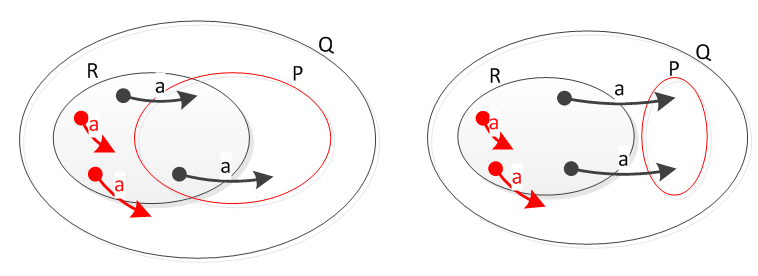
\includegraphics[width=0.8\columnwidth] {PR_1} 
	}
    \hspace{2cm}
    \subfigure[$R\cap a^{-1}P=\{q\in R|q\cdot a\in P\}$]{
    	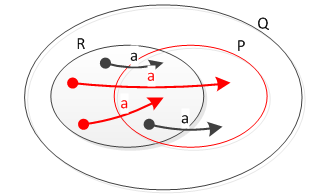
\includegraphics[width=0.4\columnwidth] {PR_2} 
    }
    \subfigure[$R\setminus a^{-1}P =\{q\in R|q\cdot a\notin P \}$]{
    	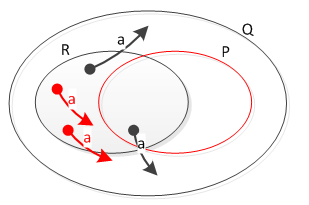
\includegraphics[width=0.4\columnwidth] {PR_3} 
    }
    \caption{$(P,a)|R=(R\cap a^{-1}P) \cup (R\setminus a^{-1}P)$}
\end{figure}

The pair $(P,a)$ is called a \textit{splitter}. Observe that $(P,a)|R=\{R\}$ if either $R\cdot a\subset P$ or $R\cdot a\cap P=\emptyset$, and $(P,a)|R$ is composed of two classes if both $R\cdot a\ne\emptyset$ and $R\cdot a\cap P^c\ne\emptyset$ or equivalently if $R\cdot a\nsubseteq P^c$ and $R\cdot a\nsubseteq P$. if $(P,a)|R$ contains two classes, then we say that $(P,a)$  \textit{splits} $R$. Note that the pair $S=(P,a)$ is called a splitter even if it does not split.

It is useful to extend the notation above to words. Given a word w and sets $P,R\subset Q$ of states, we denote by $w^{-1}P$ the set of states such that $q\cdot w\in P$, and by $(P,w)|R$ the partition of $R$ composed of the nonempty sets among
\[R\cap w^{-1}P=\{q\in R|q\cdot w\in P \} \text{ and } R\setminus w^{-1}P=\{q\in R |q\cdot w\notin P \} \]

As an example, the partition $(F,w)|Q$ is the partition of $Q$ into the set of those states from which $w$ is accepted, and the other ones. A state $q$ in one of the sets and a state $q^\prime$ in the
other are sometimes called \textit{separated} by $w$.

The Nerode equivalence is the coarsest equivalence relation on the set of states that is a (right) congruence saturating $F$. With the notation of splitters, this can be rephrased as follows.

We use later the following lemma which is already given in Hopcroft’s paper [\cite{Hopcroft71}]. It is the basic observation that ensures that Hopcroft’s algorithm works correctly.

\begin{proposition}
	The partition corresponding to the Nerode equivalence is the coarsest partition $P$ such that no splitter $(P, a)$, with $P \in \mathcal{P}$ and $a\in A$, splits a class in $\mathcal{P}$, that is	such that $(P, a)|R = \{R\}$ for all $P,R\in \mathcal{P} $and $a\in A$. $\hfill\square$
\end{proposition}

\begin{lemma}
	Let $P$ be a set of states, and let $\mathcal{P} = \{P_1, P_2\}$ be a partition of P. For any letter $a$ and for any set of states $R$, one has
	\[(P,a)|R\land (P_1,a)|R=(P,a)|R\land (P_2,a)|R=(P_1,a)|R\land (P_2,a)|R \]
	and consequntly
	\begin{align} 
	(P,a)|R \ge (P_1,a)|R\land (P_2,a)|R,\\
	(P_1,a)|R \ge (P,a)|R\land (P_2,a)|R
	\end{align}
\end{lemma}

\begin{example}
	We consider the automata given in Figure \ref{fig:revsFA} over the alphabet $A = {a, b}$.	Each automaton is the reversal of the other. However, determinization of the automaton
	on the left requires exponential time and space.
	\begin{figure}[htbp]
		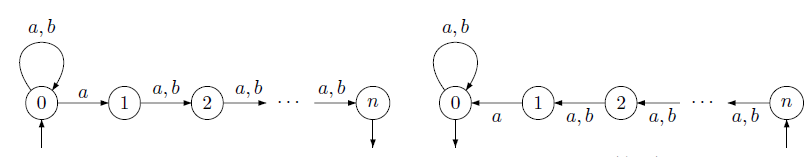
\includegraphics[scale=0.6]{revsFA}
		\caption{The automaton on the left recognizing the language $A^\ast aA^n$. It has $n + 1$ states and the minimal deterministic automaton for this language has $2^n$ states. The	automaton on the right is its reversal. It is minimal and recognizes $A^naA^\ast$.}
	    \label{fig:revsFA}
	\end{figure}
\end{example}

\subsection{Moor's algorithm}

The minimization algorithm given by Moore computes the Nerode equivalence by a stepwise refinement of some initial equivalence. All automata are assumed to be deterministic.

\begin{definition}[Moore equivalence of order $h$]
	Let $\mathcal{A}=(Q,i,F)$ be an automaton over an alphabet $A$. Define, for $q\in Q$ and $h\ge 0$, the set 
	\[L_q^{(h)}(\mathcal{A})=\{w\in A^\ast||w|\le h, q\cdot w\in F \}. \]
	The Moore equivalence of order $h$ is the equivalence $\equiv_h$ on $Q$ defined by
	\[p\equiv_h q\Leftrightarrow L_p^{(h)}(\mathcal{A})=L_q^{(h)}(\mathcal{A})\]
\end{definition}

\begin{algorithm}  
	\caption{Moore's minimization algorithm}  \label{alg:moore}
	\begin{algorithmic}%[1] %每行显示行号  
		\Require $\mathcal{A}=(Q,i,F)$  
		\Ensure The equivalence classes of $Q$  
		\State $\hat{P} \gets \{F,F^c \}$  \qquad\qquad $\triangleright$ The initial partition
		\Repeat
		\State $\hat{P}^\prime \gets \hat{P}$  \qquad\qquad $\triangleright$  $\hat{P}^\prime$ is the old partition, $\hat{P}$ is the new one
		\ForAll {$a\in A$} 
			\State $\hat{P}_a \gets \bigwedge_{P\in \hat{P}}(P,a)|Q$
		\EndFor
		\State $\hat{P}\gets \hat{P}\land \bigwedge_{a\in A}\hat{P}_a$
		\Until {$P=P^\prime$}
	\end{algorithmic}   
\end{algorithm}

The computation is described in algorithm \ref{alg:moore}. It is realized by a loop that refines the current partition. The computation of the refinement of $k$ partitions of a set swith $n$ elements can
be done in time $O(kn^2)$ by brute force. A radix sort improves the running time to $O(kn)$. With $k = Card(A)$, each tour in the loop is realized in time $O(kn)$, so the total time is $O(\mathit{l}kn)$, where $\mathit{l}$ is the number of refinement steps in the computation of the Nerode equivalence $\equiv$, that is the depth of the automaton.

The worst case behavior is obtained for $\mathit{l} = n − 2$. We say that automata having maximal depth are slow and more precisely are slow for Moore automata.

Radix sort(see, \url{https://en.wikipedia.org/wiki/Radix_sort})
In computer science, radix sort is a non-comparative integer sorting algorithm that sorts data with integer keys by grouping keys by the individual digits which share the same significant position and value.

\subsection{Hopcroft's algorithm}

Hopcroft has given an algorithm that computes the minimal automaton of a given deterministic automaton. The running time of the algorithm is $O(k n \log n)$ where $k$ the cardinality of the alphabet and $n$ is the number of states of the given automaton.

\begin{algorithm}  
	\caption{Hopcroft's minimization algorithm}  \label{alg:hopcroft}
	\begin{algorithmic}[1] %每行显示行号  
		\Require $\mathcal{A}=(Q,i,F)$  
		\Ensure The equivalence classes of $Q$  
		\State $\hat{P} \gets \{F,F^c \}$  \qquad\qquad $\triangleright$ The initial partition
		\State $W\gets \emptyset$  \qquad\qquad $\triangleright$ The waiting set
		\ForAll {$a\in A$}
			\State $ADD((min(F,F^c),a),W)$ \qquad\qquad $\triangleright$ initialization of the waiting set
		\EndFor
		\While {$W\ne\emptyset$}
			\State $(W,a)\gets TakeSome(W)$ \qquad\qquad $\triangleright$ Take and remove some splitter
			\ForAll {$P\in \hat{P}$} which is split by $(W,a)$
				\State $P^{\prime},P^{\prime\prime}\gets (W,a)|P$ \qquad\qquad $\triangleright$ Compute the split
				\State Replace $P$ by $P^\prime$ and $P^{\prime\prime}$ in $\hat{P}$ \qquad\qquad $\triangleright$ Refine the partition
			\EndFor 
			\ForAll {$b\in A$}  \qquad\qquad $\triangleright$ Update the waiting set
				\If {$(P,b)\in W$}
				  	\State Replace $(P,b)$ by $(P^\prime,b)$ and $(P^{\prime\prime})$ in $W$
				\Else
					\State $ADD((min(P^\prime,P^{\prime\prime}),b),W)$
				\EndIf  
			\EndFor
		\EndWhile
	\end{algorithmic}
\end{algorithm}

\subsubsection{Outline}

The algorithm is outlined in the function HOPCROFT given in algorithm \ref{alg:hopcroft}. We denote by $min(P, P^\prime)$ the set of smaller size of the two sets $P$ and $P^\prime$, and any one of them if they
have the same size.

Given a deterministic automaton $\mathcal{A}$, Hopcroft's algorithm computes the coarsest congruence which saturates the set $F$ of final states. It starts from the partition ${F, F^c}$ which obviously saturates $F$ and refines it until it gets a congruence. These refinements of the
partition are always obtained by splitting some class into two classes.

The algorithm proceeds as follows. It maintains a current partition $\hat{P} = {P_1,\dots,P_n}$ and a current set $W$ of splitters, that is of pairs $(W, a)$ that remain to be processed, where $W$ is a class of $\hat{P}$ and $a$ is a letter. The set $W$ is called the waiting set. The algorithm stops when the \textit{waiting} set $W$ becomes empty. When it stops, the partition $\hat{P}$ is the coarsest congruence that saturates $F$. The starting partition is the partition ${F, F^c}$ and the starting set $W$ contains all pairs $(min(F, F^c), a)$ for $a\in A$.

The main loop of the algorithm removes one splitter $(W, a)$ from the waiting set $W$ and performs the following actions. Each class $P$ of the current partition (including the class $W$) is checked as to whether it is split by the pair $(W, a)$. If $(W, a)$ does not split $P$, then nothing is done. On the other hand, if $(W, a)$ splits $P$ into say $P^\prime$ and $P^{\prime\prime}$, the class $P$ is replaced in the partition $\hat{P}$ by $P^\prime$ and $P\prime\prime$. Next, for each letter $b$, if the pair $(P, b)$ is in $W$, it is replaced in $W$ by the two pairs $(P^\prime, b)$ and $(P^{\prime\prime}, b)$, otherwise only the pair $(min(P^\prime, P^{\prime\prime}), b)$ is added to $W$.

It should be noted that the algorithm is not really deterministic because it has not been specified which pair $(W, a)$ is taken from $W$ to be processed at each iteration of the main loop. This means that for a given automaton, there are many executions of the algorithm. It turns out that all of them produce the right partition of the states. However, different executions may give rise to different sequences of splitting and also to different running time. Hopcroft has proved that the running time of any execution is bounded by $O(|A|n\log n)$.

\section{From \cite{Knuutila2001}}

\subsection{Sets,relations and mappings}

The cardinality of a set $A$ is denoted by $|A|$. 

Let $A$ and $B$ be sets and $\rho\subseteq A\times B$ a (binary) relation from $A$ to $B$. The fact that $(a,b)\in\rho (a\in A,b\in B)$ is also expressed by writing $a\rho b$. For any $a\in A$, we denote by $a\rho$ the set of elements of $B$ that are in relation $\rho$ with $a$, i.e. $a\rho=\{b\in B|a\rho b\}$. The converse of is the relation $\rho^{-1}=\{(b,a)|a\rho b\}$.Obviously $b\rho^{-1}=\{a|a\rho b\}$.

Next we consider relations on a set $A$, i.e. subsets of $A\times A$.
Theses include the diagonal relation $\omega_A=\{(a,a)|a\in A \}$, and the universal relation $\iota_A=A\times A$. The powers $\rho^n(n\ge 0)$ of a relation $\rho$ are defined as follows:
\begin{align*}
\rho^0 &=\omega_A \\
\rho^{n+1} &=\rho^n\circ \rho, \qquad n\ge 0.
\end{align*}

The relation $\rho$ is called reflexive if $\omega_A\subseteq\rho$; symmetric if $\rho^{-1}\subseteq\rho$; and transitive if $\rho^2\subseteq\rho$.

A relation on $A$ is called an \textit{equivalence relation} on $A$, if it is reflexive, symmetric and transitive. The set of all equivalence relations on a set $A$ is denoted by $Eq(A)$. It is obvious that both $\omega_A\in Eq(A)$ and $\iota_A \in Eq(A)$. Let $\rho\in Eq(A)$. The $\rho$-class $a\rho$ of an element $a (\in A)$ is also denoted by $a/\rho$. The \textit{quotient set} or the \textit{partition of A} with
respect to $\rho$, is $A/\rho=\{a\rho|a\in A \}$. If $\pi\in Eq(A)$ and $\pi\subset \rho$, then the partition $A/\pi$ is a \textit{refinement} of $A/\rho$ (each $\rho$-class is a union of some $\pi$-classes); this is also expressed by saying that $\pi$ is \textit{finer} than $\rho$ or that $\rho$ is \textit{coarser} than $\pi$. We often define an equivalence relation $\rho$ on $A$ via the set $A/\rho$, i.e. in the form $A/\rho=\{C_1,\dots,C_m \}$, where the sets $C_i$ are the classes of $\rho$.

The cardinality of $A/\rho$ is called the \textit{index} of $\rho$; especially, if $A/\rho$ is finite, then is said to have a  \textit{finite index}. For any subset $H$ of $A$, $H/\rho$ denotes $\{a\rho|a\in H \}$. The equivalence $\rho$ saturates the subset $H$, if $H$ is the union of some $\rho$-classes. Hence, $\rho$ saturates $H$ iff $a\rho\in H/\rho$ implies $a\rho\subseteq H$.

A \textit{mapping} or a \textit{function} $\phi:A\to B$ is a relation $\phi\subseteq A\times B$ such that $|a\phi|=1$ for all $a\in A$. If $a\phi b$, then $b$ is the \textit{image} of $a$ and $a$ is a \textit{preimage} of $b$. That $b$ is an image of $a$ is expressed by writing $b=\phi(a)$ and that $a$ is a preimage of $b$ is written as $a=\phi^{-1}(b)$. The notation $a=\phi^{-1}(b)$ is justified合理的, when  $\phi$  is bijective (see below). The \textit{restriction} of a mapping $\phi:A\to B$ to a set $C\subseteq  A$ is the mapping $\phi|C:C\to B$ where $\phi|C=\phi\cap(C\times B)$.

The \textit{composition} of two mappings $\phi:A\to B$ and $\psi:B\to C$ is the mapping
$\phi\psi: A\to C$, where $\phi\psi$ is the product of $\phi$ and $\psi$ as relations. The \textit{kernel} $\phi\phi^{-1}$ of a mapping $\phi:A\to B$, also denoted by $\ker\phi$, is an equivalence relation on $A$ and $a\phi\phi^{-1}b$ iff $a\phi=b\phi (a,b\in A)$. A mapping $\phi:A\to B$ is called \textit{injective} if $\ker \phi=\omega_A$; \textit{surjective} (or onto) if $A\phi =B$; and \textit{bijective} if it is both injective and surjective.

\begin{figure}[htbp]
	\subfigure[An injective non-surjectice function(injection, not a bijection) ]{
		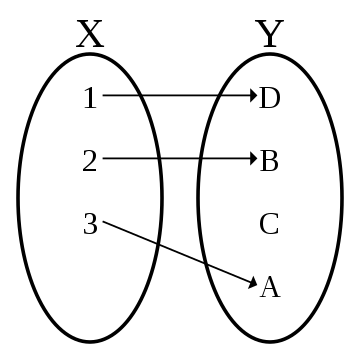
\includegraphics[width=0.2\columnwidth] {Injection} 
	}
	\subfigure[An injective surjective function (bijection) ]{
		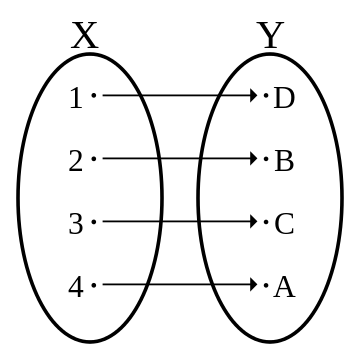
\includegraphics[width=0.2\columnwidth] {Bijection} 
	}
    \subfigure[A non-injective surjective function (surjection, not a bijection) ]{
    	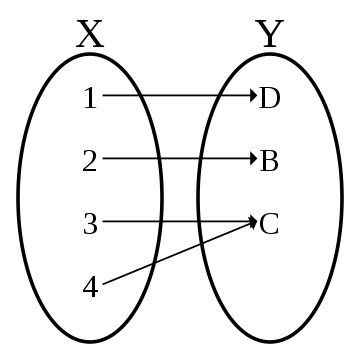
\includegraphics[width=0.2\columnwidth] {Surjection} 
    }
	\subfigure[A non-injective non-surjective function (also not a bijection) ]{
		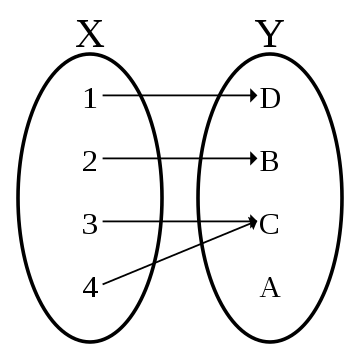
\includegraphics[width=0.2\columnwidth] {Not-Injection-Surjection} 
	}
\caption{The term one-to-one function must not be confused with one-to-one correspondence (a.k.a. bijective function), which uniquely maps all elements in both domain and codomain to each other}
\end{figure}

\subsection{Preliminaries}

\begin{definition}[$a\rho_Gb$]
	DFA $G=(Q,\Sigma,\delta,q_0,F)$, Two states $a$ and $b$ of $G$ are equivalent, which we express by writing $a\rho_G b$, if 
	\[(\forall w\in \Sigma^\ast) (\delta(a,w)\in F)\Leftrightarrow\delta(b,w)\in F) \]
\end{definition}

\begin{definition}[$\omega_Q,\iota_Q,Eq(Q)$]
	DFA $G=(Q,\Sigma,\delta,q_0,F)$, the diagonal relation $\omega_Q=\{(a,a)|a\in Q \}$, the universal relation $\iota_Q=Q\times Q$. The set of all equivalence relations on a set $Q$ is denoted by $Eq(Q)$. It is obvious that both $\omega_Q\in Eq(Q)$ and $\iota_Q \in Eq(Q)$. 
\end{definition}

\begin{definition}[the reduced $G$]
	DFA $G$ is reduced, if $a\rho_G b$ implies $a=b$, i.e. $\rho_G=\omega_Q$
\end{definition}

\begin{definition}[$Con(G)$]
	A relation $\rho\in Eq(Q)$ is a congruence of $G$, if 
	\begin{enumerate}[(1) ]
		\item $a\rho b$ implies $\delta(a,x)\rho\delta(b,x)$ for all $a,b\in Q$ and all $x\in \Sigma$, and
		\item $\rho$ saturates $F$ 
	\end{enumerate} 
	We denote by $Con(G)$ the set of all congruences of $G$. 
\end{definition}

\begin{definition}[quotient DFA $G/\rho$]
	It is well-known that the relation $\rho_G$ is the greatest (coarsest)  congruence of $G$. For any $\rho\in Con(G)$ the quotient DFA $G/\rho$ is defined as $G/\rho=(Q/\rho,\Sigma,\delta/\rho,q_0/\rho,F/\rho)$ where $\delta/\rho(a/\rho,x)=\delta(a,x)/\rho$. 
\end{definition}

\begin{definition}[DFA as unary algebras]
	DFA $G=(Q,\Sigma,\delta,q_0,F)$, $\Sigma$ is viewed as a set of unary operation symbols and the transition function $\delta$ of $G$ is replaced by the $\Sigma$-indexed family $(x^G:x\in\Sigma)$ of unary operations which are defined so that for any $x\in\Sigma$ and $a\in Q, x^G(a)=\delta(a,x)$. We shall omit $G$ from the superscript and write simply $x(a)$ for $\delta(a,x)$. 
	
	Clearly, a string $w=x_1x_2\dots x_n$ is accepted by $G$ if and only if $x_n(\dots(x_2(x_1(q_0))\dots)\in F$. 
\end{definition}

\subsection{The classical algorithm}

The classical minimization algorithm is based on the following ``layer-wise' definition for the equivalence relation $\rho_G$.

\begin{proposition} \label{pro:eq}
	Let $G=(Q,\Sigma,\delta,q_0,F)$ and a series $\rho_i (i\ge 0)$ of equivalence relations on $Q$ be defined as follows:
	\begin{align*}
	\rho_0 &=\{(a,b)|a,b\in F \} \cup \{(a,b)|a,b\in Q-F \},\\
	\rho_{i+1} &=\{(a,b)\in\rho_i|(\forall x\in \Sigma) (\delta(a,x),\delta(b,x))\in\rho_i \}
	\end{align*}
	Then the following hold.
	\begin{enumerate} [(1) ]
		\item $\rho_0\supseteq\rho_1\supseteq\cdots$
		\item If $\rho_i=\rho_{i+1}$ then $\rho_i=\rho_{i+j}$ for all $j>0$ and furthermore, $\rho_i=\rho_G$.
		\item There exists $0\le k\le |Q|$ such that $\rho_k=\rho_{k+1}$. 
	\end{enumerate}
\end{proposition}

\textbf{ The refinements on individual classes}

When the construction of Proposition \ref{pro:eq} is implemented, each refinement step leading from $\rho_i$ to $\rho_{i+1}$ consists of a series of refinements on individual classes of $\rho_i$. The refinement of a single class $B$ can be implemented with suitably chosen data structures for equivalence relations to run in time $O(|\Sigma||B|)$, and each refinement from $\rho_i$ to $\rho_{i+1}$
takes thus time $O(|\Sigma||Q|)$.

\begin{example}
	We construct (the worst kind of ) a DFA Fig. \ref{fig:mini-ex1_1}.
	
	\begin{align*}
		G/\rho_0&=\{\{6\},\{1,2,3,4,5\} \}, \\
		B &= \{1,2,3,4,5 \}, \delta(5,0)\notin B,\delta(i,0)=i+1\in B,1\le i \le 4,\\
		G/\rho_1&=\{\{6\},\{5\}, \{1,2,3,4 \} \} \\
		B &= \{1,2,3,4 \}, \delta(4,0)\notin B,\delta(i,0)=i+1\in B,1\le i \le 3,\\
		G/\rho_2&=\{\{6\},\{5\}, \{4\}, \{1,2,3\} \} \\
		B &= \{1,2,3 \}, \delta(3,0)\notin B,\delta(i,0)=i+1\in B,1\le i \le 2,\\
		G/\rho_3&=\{\{6\},\{5\}, \{4\}, \{3\},\{1,2\} \} \\
		B &= \{1,2 \}, \delta(2,0)\notin B,\delta(i,0)=i+1\in B,1\le i \le 1,\\
		G/\rho_4&=\{\{6\},\{5\}, \{4\}, \{3\},\{2\},\{1\} \} 
	\end{align*}
	
	The classical minimization algorithm is ineffective, since in the worst kind of a DFA, each refinement step from $\rho_i$ to $\rho_{i+1}$ removes always one state from the only nonsingleton class. The work performed by the algorithm (even if we optimize it to avoid considering singleton classes) will then be proportional to $|\Sigma|\sum_{i=1}^{|Q|-2}(|Q|-i)$, which leads to $O(|\Sigma||Q|^2)$ execution time.
	
	\begin{figure}[htbp]
		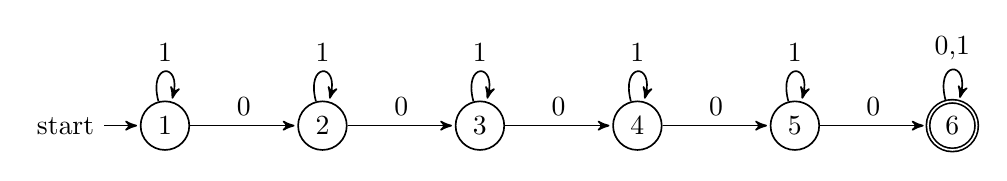
\begin{tikzpicture}[->,>=stealth',shorten >=1pt,auto,node distance=2cm, semithick]
		\tikzstyle{every state}=[minimum size=0.1mm]
		\node[initial,state] (p1)  {$1$};
		\node[state]         (p2) [right of=p1] {$2$};
		\node[state]         (p3) [right of=p2] {$3$};
		\node[state]         (p4) [right of=p3] {$4$};
		\node[state]         (p5) [right of=p4] {$5$};
		\node[state,accepting] (p6) [right of=p5] {$6$};
		\path
		(p1) edge [loop above] node {1} (p1)
		edge [] node {0} (p2)
		(p2) edge [loop above] node {1} (p2)
		edge [] node {0} (p3)
		(p3) edge [loop above] node {1} (p3)
		edge [] node {0} (p4)
		(p4) edge [loop above] node {1} (p4)
		edge [] node {0} (p5)
		(p5) edge [loop above] node {1} (p5)
		edge [] node {0} (p6)
		(p6) edge [loop above] node {0,1} (p6)
		;
		\end{tikzpicture}
		\caption{Minimizing example} \label{fig:mini-ex1_1}
	\end{figure}
\end{example}

\subsection{Atomic refinements}

Note that the construction of Proposition \ref{pro:eq}  reaches the situation $\rho_i = \rho_{i+1}$ when $\rho_i$ becomes a congruence, i.e. 
\[(\forall a,b\in Q, x\in Q) a\rho_i b\implies \delta(a,x)\rho_i\delta(b,x) \]. 

Now consider the situation where $\rho_i \ne \rho_{i+1}$. Obviously,
\begin{align*}
\rho_i\ne\rho_{i+1} &\Leftrightarrow (\exists a,b\in Q,x\in\Sigma) &(a,b)\in\rho_i \text{ and } (\delta(a,x),\delta(b,x))\notin\rho_i\\
&\Leftrightarrow (\exists B\in Q/\rho_i,x\in\Sigma) &(a,b)\in B  \text{ and } (\delta(a,x),\delta(b,x))\notin\rho_i\\
&\Leftrightarrow (\exists B,C\in Q/\rho_i,x\in\Sigma) &(a,b)\in B  \text{ and } \delta(a,x)\in C, \text{ and } \delta(b,x))\notin C\\
&\Leftrightarrow (\exists B,C\in Q/\rho_i,x\in\Sigma) &(a,b)\in B  \text{ and } \delta(B,x)\cap C\ne\emptyset, \text{ and } \delta(B,x))\nsubseteq C
\end{align*}

The step from $\rho_i$ to $\rho_{i+1}$ can thus be understood as a series of ``atomic' refinements performed for such $x\in \Sigma, B,C\in Q/\rho_i$ that
\begin{equation}\label{equ:atomic}
	\delta(B,x)\cap C\ne\emptyset \text{ and } \delta(B,x))\nsubseteq C
\end{equation}
holds, Each such atomic refinement partition then $B$ into $B\cap x^{-1}(C) \}$ and $B-(B\cap x^{-1}C))$. We denote these refinements of $B$ with $B_{C,x}$ and $B^{C,x}$, respectively. We use the notation $B^\prime$ and $B^{\prime\prime}$ for these refinements of $B$ when their relation to the pair $(C,x)$ has no importance.

Let us next rewrite Proposition \ref{pro:eq} in the terms of these atomic refinements.

\begin{proposition} \label{pro:eq_relations}
	Let $G=(Q,\Sigma,\delta,q_0,F)$ be a DFA and series $\theta_i (i\ge 0)$ of equivalence relation on $Q$ be defined as follows:
	\begin{align*}
		Q/\theta_0 &=\{F,Q-F \}, &\\
		Q/\theta_{i+1} &=\begin{cases}
		(Q/\theta_i-\{B\})\cup\{B_{C,x},B^{C,x}\} &\text{ if \ref{equ:atomic} holds for some } B,C\in Q/\theta_i, x\in\Sigma,\\
		Q/\theta_i &\text{otherwise}.
		\end{cases}
	\end{align*}
	Then there exists a $k\le |Q|$ such that $\theta_{i+l}=\theta_i$ for all $l\ge 0$ and $\theta_k=\rho_G$.
\end{proposition}

\begin{proof}
	The upper bound comes from the observation, that each atomic refinement increases the index of $\theta_i$ by one. Naturally this index cannot be increased more than $|Q|-1$ times.
	
	It is clear that $\theta_k$ is both an equivalence relation saturating $F$ (it is a refinement of $\theta_0$) and a congruence of $G$ (since Eq. (\ref{equ:atomic}) does not hold for $\theta_k$). What remains, is to show that $\theta_k$ is also the \textit{greatest} congruence $\rho_G$ of $G$.
	
	We show first that $\theta_i\supseteq\rho_G$ for all $i\ge 0$. When contraposed, the claim is that if $(a,b)\notin\theta_i$ then $(a,b)\notin\rho_G$ (for all $i\ge 0$). This is clearly true for $\theta_0$, since final and non-final states are not in $\rho_G$. Suppose then that the claim holds for all $0\le l\le i$ and let $(a,b)\in\theta_i$. If $(a,b)\notin\theta_{i+l}$, it must be the case that for some $x\in\Sigma,(x(a),x(b))\notin\theta_i $. 
	But this implies (by IA) that $x(a)$ and $x(b)$ are not in $\rho_G$. Thus, $a$ and $b$ become inequivalent in $\theta_{i+l}$ only when they are shown to be inequivalent in $\rho_G$, formally $(a,b)\notin\theta_{i+l}\implies (a,b)\notin\rho_G$. 
	
	It now holds that $\theta_0\supseteq\theta_1\supseteq\cdots\supseteq\theta_k$ (by definition), and consequently $\theta_0\supseteq\theta_1\supseteq\cdots\supseteq\theta_k\supseteq\rho_G$. Since $\rho_G$ is the greatest congruence of $G$, and $\theta_k$ is a congruence, it must be the case that $\theta_k=\rho_G$.  $\hfill\square$.
\end{proof}

Note that the construction given in Proposition \ref{pro:eq_relations} does not fix the order in which the triples $B, C, x$ are exploited to refine $\theta_i$. Thus, all the different orderings yield the same result at the end: the unique greatest congruence.

\begin{algorithm}  
	\caption{Comuting $\rho_G$ using atomic refinements}  \label{alg:atomic}
	\begin{algorithmic}[1] %每行显示行号  
		\Function {Equivalence} {$G$}
		\State $Q/\theta\gets \{F,Q-F\}$
		
		\While {($\exists B,C\in Q/\theta,x\in\Sigma$ s.t. Eq. \ref{equ:atomic} holds)}
		\State $Q/\theta\gets(Q/\theta-\{B\}\cup\{B_{C,x},B^{C,x}  \}$
		\EndWhile
		
		\State \Return{$\theta$}  
		\EndFunction 
	\end{algorithmic}
\end{algorithm}

How to efficiently find some triple $B,C,x$ for which Eq. (\ref{equ:atomic}) holds.

The refiners of $B$ in $\theta$, shortly $ref(B,\theta)$:
\[ref(B,\theta)=\{(C,x)\in(Q/\theta)\times\Sigma|x(B)\cap C\ne\emptyset \text{ and } x(B)\nsubseteq C \} \]

As each $B$ is related to $ref(B,\theta)$, so is each pair $(C,x)$ related to its \textit{objects of refinement} in $\theta$,
\[obj(C,x,\theta)=\{B\in Q/\theta|(C,x)\in ref(B,\theta) \} \]

\begin{algorithm}  
	\caption{Refiner-driven implementation}  \label{alg:refiner-driven}
	\begin{algorithmic}[1] %每行显示行号  
		\Function {Equivalence} {$G$}
		\State $Q/\theta\gets \{F,Q-F\}$
		
		\While {($\exists some(C,x)\in(Q/\theta)\times\Sigma$ with $obj(C,x,\theta)\ne\emptyset$)}
		\For {$B\in obj(C,x,\theta)$}
			\State replace $B$ with $B_{C,x}$ and $B^{C,x}\in Q/\theta$
		\EndFor
		\EndWhile
		
		\State \Return{$\theta$}  
		\EndFunction 
	\end{algorithmic}
\end{algorithm}

\begin{lemma} \label{lemma:refine_B}
	Let $G=(Q,\Sigma,\delta,q_0,F),\theta\in Eq(Q)$ and $B,C\in Q/\theta$ and $x\in\Sigma$. Suppose we refine $B\in Q/\theta$ into $B_{C,x}$ and $B^{C,x}$ with respect to $(C,x)$. Let $D$ be a subset of $B_{C,x}$ or $B^{C,x}$, then $D\notin(C,x,\theta)$.
\end{lemma}

\begin{proof}
	Let us first condider the case $D\in\{B_{C,x},B^{C,x}\}$. Then either $x(a)\in C$ for all $a\in D$ or $x(a)\notin C$ for all $a\in D$. The same property holds naturally for all subsets of $D$.
\end{proof}

The bookkeeping needed for telling whether a particular pair $(C,x)$ has been used can be implemented as follows:
\begin{itemize}
	\item We maintain a set $L$ of candidate refiners, shortly candidates, in $(Q/\theta)\times\Sigma$. Initially $L=\{F,Q-F\}\times X$.
	\item Pairs $(C,x)$ are now selected from $L$, not (blindly) from all of $(Q/\theta)\times\Sigma$.
	\item Every time we select a pair $(C,x)$ from $L$, we remove it from $L$. This is justified by Lemma \ref{lemma:refine_B}.
	\item After refining $\theta$ to $\theta^\prime$, we must also update $L$ to contain only classes of $\theta^\prime$. We do the following for each $x\in\Sigma$ and each class $B$ refined to $B^\prime$ and $B^{\prime\prime}$:
	\begin{itemize}
		\item[$\circ$] if $(B,x)\in L$, we remove $(B,x)$ and add both $(B^\prime,x) and (B^{\prime\prime},x)$ to $L$. This is (indirectly) justified by Proposition \ref{pro:eq_relations}, since only the current $\theta$-classes are used in the construction.	
		\item[$\circ$] If $(B,x)\notin L$, we simply add $(B^\prime)$ and $(B^{\prime\prime})$ to $L$.
	\end{itemize}
\end{itemize}

Note that new items are inserted into $L$ only when some class gets refined. Thus, $L$ will eventually become empty, because each iteration removes one element from $L$, and the total number of elements added into $L$ is bounded by $2|\Sigma||Q|$ (the maximum number of different equivalence classes created in any refinement sequence is $2|Q|-1$. The ideas above are collected into Algorithm \ref{alg:set-driven}.

\begin{algorithm}  
	\caption{Set-driven implementation}  \label{alg:set-driven}
	\begin{algorithmic}[1] %每行显示行号  
		\Function {Equivalence} {$G$}
		\State $Q/\theta\gets \{F,Q-F\}$
		\State $L\gets (Q/\theta)\times\Sigma$
		
		\While {$L\ne\emptyset$}
		\State remove a pair $(C,x)$ from $L$
		\ForAll {$B\in obj(C,x,\theta)$}
			\State replace $B$ with $B_{C,x}$ and $B^{C,x}$ in  $Q/\theta$
			\ForAll {$y\in\Sigma$}
				\If {$(B,y)\in L$}
					\State replace $(B,y)$ with $(B^\prime,y)$ and $(B^{\prime\prime},y)$ in $L$
				\Else
					\State insert $(B^\prime,y)$ and $(B^{\prime\prime},y)$ to $L$
				\EndIf
			\EndFor
		\EndFor
		\EndWhile
		
		\State \Return{$\theta$}  
		\EndFunction 
	\end{algorithmic}
\end{algorithm}

\begin{lemma} \label{lemma:refine}
	Let $G=(Q,\Sigma,\delta,q_0,F),\theta\in Eq(Q)$ and $B\in Q/\theta$. Suppose we refine $B$ into $B^\prime$ and $B^{\prime\prime}$. Then, for any $y\in\Sigma$, refining all the classes of $\theta$ with respect to any two of the pairs $(B,y),(B^\prime,y)$ and $(B^{\prime\prime})$ gives the same result as refining them with respect to all three of them.
\end{lemma}

\begin{proof}
	Consider an arbitrary class $D\in Q/\theta, a\in D$ and $y\in\Sigma$. As seen in Fig. \ref{fig:refine}, the transition $\delta(a,y)$ satisfies exactly one of the following: 
	\begin{enumerate}[(1) ]
		\item $\delta(a,y)\in B^\prime$
		\item $\delta(a,y)\in B^{\prime\prime}$
		\item $\delta(a,y)\notin B$
	\end{enumerate}
	Now each possible refinement sequence with respect to any two of the sets $B,B^\prime$ and $B^{\prime\prime}$ and letter $y$ partitions $D$ into $D_1,D_2,D_3$, which is the same as the result yielded by performing all the three refinements.
\end{proof}

\begin{figure}[htbp]
	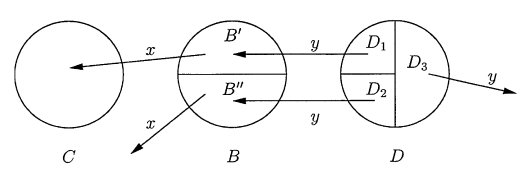
\includegraphics[scale=0.6]{refine}
	\caption{Illustration of Lemma \ref{lemma:refine}}
	\label{fig:refine}
\end{figure}

%%%%%%%%%%%%%%%%%%%%%%%%%%%%%%%%%%%%%%%%%%%%%%%%%%
\begin{thebibliography}{99}
	\bibitem[Hopcroft71]{Hopcroft71}
	Hopcroft, J.E. \textit{An n log n algorithm for minimizing states in a finite automaton}, in The Theory of Machines and Computations (Z. Kohavi, ed.), pp.180-196, Academic Press, New York, 1971.
	
	\bibitem[Gries73]{Gries73}
	Gries, D. \textit{Describing an Algorithm by Hopcroft}, Acta Inf. 2:97 109, 173. $\copyright$ by Springer-Verlag 1973
	
	\bibitem[Knuutila2001]{Knuutila2001}
	Knuutila, T. \textit{Re-describing an Algorithm by Hopcroft}. Theoret. Computer Science 250 (2001) 333--363.
		
	\bibitem[Ratnesh95]{Ratnesh95}
	Ratnesh Kumar, \textit{Modeling and Control of Logical Discrete Event Systems}, $\copyright$ 1995 by Springer Science+Business Media New York.
	
	\bibitem[Jean2011]{Jean2011}
	Jean Berstel, Luc Boasson, Olivier Carton, Isabelle Fagnot
	, \textit{Minimization of automata}, Universit$\acute{e}$ Paris-Est Marne-la-Vall$\acute{e}$e 2010 Mathematics Subject Classification: 68Q45, 2011.
	
	\bibitem[Kenneth2012]{Kenneth2012}
	Kenneth H. Rosen著,徐六通译, \textit{离散数学及其应用Discrete Mathematics and Its Applications},seventh Edition, 2012, 机械工业出版社, 北京, 2014.
	
\end{thebibliography}

%\chapter{\cite{蒋宗礼2013}(第1章 绪论)}

\begin{itemize}
	\item 集合:集合的表示、集合之间的关系、集合的基本运算。
	\item 关系:主要介绍了二元关系相关的内容。包括等价关系、等价分类、关系合成、关系闭包。
	\item 递归定义与归纳证明。	
	\item 图:无向图、有向图、树的基本概念。
	\item 语言与形式语言:自然语言的描述,形式语言和自动机理论的出现,形式语言和自动机理论对计算机科学与技术学科人才能力培养的作用
	\item 基本概念:字母表、字母、句子、字母表上的语言、语言的基本运算
	
\end{itemize}

\section{集合的基础知识}
\subsection{集合之间的关系}
\begin{definition}
	设$A,B$是两个集合,如果集合$A$中的元素都是集合$B$的元素,则称集合$A$是集合$B$的\emph{子集(subset)},集合$B$是集合$A$的\emph{包集(container)}。记作$A\subseteq B$,也可以记作$B\supseteq A$。
\end{definition}

由定义可知,$A\subseteq B$的充要条件是:对于A中的每一个元素$a$,均有$a\in B$。为了简洁起见,$P_1$是$P_2$的充要条件记为
$$P_1\iff P_2$$
或者
$$P_2\text{ iff }P_1$$

经常使用全称量词和存在量词:$\forall x$表示对所有的$x$; $\exists x$表示存在一个$x$。
按照此约定,有

$A\subseteq B\iff\forall x\in A,x\in B$成立,\\
也就是

$A\subseteq B\text{ iff }\forall x\in A,x\in B$成立。

\begin{definition}
	设$A,B$是两个集合,如果$A\subseteq B,\text{且}\exists x\in B,\text{但}x\notin B$,则称$A$是$B$的\emph{真子集(proper subset)},记作$A\subset B$。
\end{definition}

\begin{definition}
	如果集合$A,B$含有的元素完全相同,则称集合$A$与集合$B$\emph{相等(equivalence)},记作$A=B$。
\end{definition}

对任意集合$A,B,C$,不难得出下列结论:
\begin{enumerate}
	\item $A=B$ iff $A\subseteq B$且$B\subseteq A$。
	\item 如果$A\subseteq B$,则$|A|\le|B|$。
	\item 如果$A\subset B$,则$|A|\le|B|$。
	\item 如果A是有穷集,且$A\supset B$,则$|B|>|A|$。
	\item 如果$A\subseteq B$,则$\forall x\in A$,有$x\in B$。
	\item 如果$A\subset B$,则$\forall x\in A$,有$x\in B$并且$\exists x\in B$,但$x\notin A$。
	\item 如果$A\subseteq B$且$B\subseteq C$,则$A\subseteq C$。
	\item 如果$A\subset B$且$B\subset C$,或者$A\subseteq B$且$B\subset C$,或者$A\subset B$且$B\subseteq C$,则$A\subset C$。
	\item 如果$A=B$,则$|A|=|B|$。
\end{enumerate} 

\begin{definition}
	设$A,B$是两个集合,$A$与$B$的\emph{对称差(symmetric difference)}是一个集合,该集合由属于$A$但不属于$B$,以及属于$B$但不属于$A$的所有元素组成,记作$A\otimes B$。
	$$A\otimes B = \{a|a\in A\text{且}a\notin B\text{或者}a\notin B\text{且}a\in B\}$$
\end{definition}

显然,对集合$A,B$,有
$$A\otimes B = (A\cup B) - (A\cap B) = (A-B)\cup(B-A)$$

$\otimes$为对称差运算符,$A\otimes B$读作$A$对称减$B$($A$与$B$的对称差)。

\begin{definition}
	设$A,B$是两个集合,$A$与$B$的\emph{笛卡儿积(Cartesian product)}是一个集合,该集合该集合是由所有这样的有序对$(a,b)$组成的:其中$a\in A,b\in B$ ,记作$A\times B$。
	$$A\times B = \{(a,b)|a\in A \& b\in B\}$$
\end{definition}
$\times$为笛卡儿乘运算符。$A\times B$读作$A$叉乘$B$。

对任意集合$A,B,C$,不难得出下列结论:
\begin{enumerate}
	\item $A\times B\ne B\times A$。
	\item $(A\times B)\times C\ne A\times(B\times C)$。
	\item $A\times A\ne A$。
	\item $A\times\emptyset=\emptyset$。
	\item $A\times(B\cup C)=(A\times B)\cup(A\times C)$。
	\item $(B\cup C)\times A=(B\times A)\cup(C\times A)$。
	\item $A\times(B\cap C)=(A\times B)\cap(A\times C)$。
	\item $(B\cap C)\times A=(B\times A)\cap(C\times A)$。
	\item $A\times(B-C)=(A\times B)-(A\times C)$。
	\item $(B-C)\times A=(B\times A)-(C\times A)$。
	\item 当$A,B$为有穷集时,$|A\times B|=|A||B|$。
\end{enumerate} 

\begin{definition}
	设$A$是一个集合,$A$的\emph{幂集(power set)}是一个集合,该集合由$A$的所有子集组成,记作$2^A$。
	$$2^A=\{B|B\subseteq A\}$$
\end{definition}
$2^A$读作$A$的幂集。

对于任意集合$A,B$,则有下列结论:
\begin{enumerate}
	\item $\emptyset\in 2^A$。
	\item $\emptyset\subseteq 2^A$。
	\item $\emptyset\subset 2^2$。
	\item $2^\emptyset=\{\emptyset\}$。
	\item $A\in 2^A$。
	\item 如果$A$是有穷集合,则$|2^A|=2^|A|$。
	\item $2^{A\cap B} = 2^A\cap 2^B$。
	\item if $A\subseteq B$, then $2^A\subseteq 2^B$。
\end{enumerate}


\begin{definition}
	设$A$是论域$U$上的一个集合,$A$的\emph{补集(complementary set)}是一个集合,该集合由在$U$中,但不在$A$中的所有元素组成,记作$\bar{A}$。
	$$\bar{A}=U-A$$
\end{definition}
$\bar{A}$读作$A$(关于论域$U$)的补集($U$中子集$A$的补集)。

在实际工作和生活中,人们都会在一定的范围内讨论问题,讨论问题的这个范围叫作论域。如果集合$A$是论域$U$上的一个集合,则$A\subseteq U$。

设$U$是论域,$A,B$是$U$上的集合,则有下列结论:
\begin{enumerate}
	\item $\bar{\emptyset}=U$。
	\item $\bar{U}=\emptyset$。
	\item if $A\subseteq B$, then $\bar{B}\subseteq \bar{A}$。
	\item $A\cup \bar{A}=U$。
	\item $A\cap \bar{A}=\emptyset$。
	\item $B=\bar{A}\iff A\cup B=U\& A\cap B=\emptyset$。
	\item De Morgan定律\\ 
	$\overline{A\cap B}=\bar{A}\cup\bar{B}$。\\
	$\overline{A\cup B}=\bar{A}\cap\bar{B}$。
\end{enumerate}


\section{关系}
\begin{itemize}
	\item 二元关系 
	\item 递归定义与归纳证明 
	\item 关系的闭包 
\end{itemize}

\subsection{二元关系}

\begin{definition}
	设$A,B$是两个集合,任意的$R\subset A\times B,R$是$A$到$B$的\emph{二元关系(binary relation)}。
	
	$(a,b)\in R$,表示$a$与$b$满足关系$R$,按照中缀形式,也可以表示为$aRb$。
	
	$A$称为\emph{定义域(domain)}, $B$称为\emph{值域(range)}。
	
	当$A=B$时,则称$R$是$A$上的二元关系。
\end{definition}

\begin{definition}
	$R$是$A$上的二元关系,
	\begin{enumerate}
		\item 如果对任意一个$a\in A$,有$(a,a)\in R$,则称$R$是\emph{自反的(reflexive)}。
		\item 如果对任意一个$a\in A$,有$(a,a)\notin R$,则称$R$是\emph{反自反的(irreflexive)}。
		\item 如果对任意的$a,b\in A$,当$(b,a)\in R$时,必有$(a,b)\in R$,
		则称$R$是\emph{对称的(symmetric)}。
		\item 如果对任意的$a,b\in A$,当$(b,a)\in R$和$(a,b)\in R$同时成立,必有$a=b$,
		则称$R$是\emph{反对称的(asymmetric)}。
		\item 如果对任意的$a,b,c\in A$,当$(a,b)\in R$和$(b,c)\in R$同时成立,必有$(a,c)\in R$,
		则称$R$是\emph{传递的(transition)}。
	\end{enumerate}
    条件(1),(3),(5)合并在一起,叫作关系的三歧性:自反性,对称性,传递性。
\end{definition}

\begin{example}
	关系的性质。
	\begin{enumerate}
		\item $=$关系是自反的,对称的,传递的。
		\item $>,<$关系是反自反的,传递的。
		\item $\ge,\le$关系是自反的,反对称的,传递的。
		\item 集合之间的包含关系是自反的,反对称的,传递的。
		\item 整数集上的模$n$同余关系是自反的,对称的,传递的。
		\item 通常意义下的父子关系是反自反的,非传递的。
		\item 通常意义下的兄弟关系是反自反的,传递的。
		\item 通常意义下的祖先关系是反自反的,传递的。
	\end{enumerate}
\end{example}

\subsection{等价关系与等价类}

\begin{definition}
	如果集合$A$上的二元关系$R$是自反的,对称的,传递的,则称$R$是\emph{等价关系(equivalence relation)}。
\end{definition}

\begin{example}
	等价关系示例。
	\begin{enumerate}
		\item 实数集上的“=”关系。
		\item 整数集上的模$n$同余关系。
		\item 通常意义下的“在同一个学校工作”的关系。
		\item “户口在同一省、市、自治区”的关系。
	\end{enumerate}
    由此,可以考虑利用集合$S$上的等价关系$R$将$S$划分成若干个等价类。
\end{example}

\begin{definition}
	设$R$是集合$S$上的等价关系,则满足如下要求的$S$的划分$S_1,S_2,S_3,\cdots,S_n,\cdots$称为$S$关于$R$的等价划分,$S_i$称为\emph{等价类(equivalence class)}。它们满足以下各条:
	\begin{enumerate}
		\item $S=S_1\cup S_2\cup S_3\cup\cdots\cup S_n\cup\cdots$。
		\item if $i\ne j$, then $S_i\cap S_j=\emptyset$。
		\item 对任意的$i,S_i$中的任意两个元素$a,b,aRb$恒成立。
		\item 对任意的$i,j,i\ne j,S_i$中的任意元素$a$和$S_j$中的任意元素$b,aRb$恒不成立。
	\end{enumerate}

    $R$将$S$分成的等价类的个数称为$R$在$S$上的\emph{指数(index)}。有时候,$R$将$S$分成有穷多个等价类,此时称$R$具有有穷指数,反之称为无穷指数。
\end{definition}

\begin{example} 等价类。
	\begin{enumerate}
		\item "="关系将自然数$\mathbb{N}$分成无穷多个等价类:$\{1\},\{2\},\{3\},\cdots$。
		\item 非负整数集上的模5同余关系将$\{0,1,2,3,\cdots\}$分成5个等价类:\\
		$\{0,5,10,15,20,\cdots\}$\\
		$\{1,6,11,16,21,\cdots\}$\\
		$\{2,7,12,17,22,\cdots\}$\\
		$\{3,8,13,18,23,\cdots\}$\\
		$\{4,9,14,19,24,\cdots\}$
		\item 某计算机学院2001年招收本科生420名,分成12个班,按同班同学关系划分,这420名学生分成12个等价类,每个等价类对应一个班。
	\end{enumerate}
\end{example}

\begin{note}
值得注意的是,给定集合$S$上的一个等价关系$R$,$R$就确定了$S$的一个等价划分。当给定另一个不同的等价关系时,它会确定$S$的一个新的等价划分。
\end{note}

\begin{example}令$S=\{1,2,3,4\}$.
	\begin{enumerate}
		\item 通常意义的"="关系将$S$分成4个等价类:$\{1\},\{2\},\{3\},\{4\}$。
		\item 如果取$R=\{(1,1),(2,1),(1,2),(2,2),(3,3),(3,4),(4,3),(4,4)\}$,则将$S$分成两个等价类:$\{1,2\},\{3,4\}$。
		
		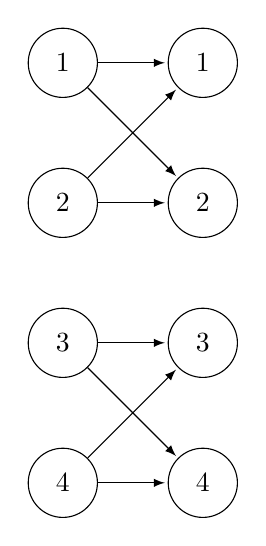
\begin{tikzpicture}[>=latex, shorten >=1pt,node distance=0.7in, on grid, auto]
		\node[state] (q1) {$1$};
		\node[state] (q2) [below of=q1] {$2$};
		\node[state] (q3) [below of=q2] {$3$};
		\node[state] (q4) [below of=q3] {$4$};
		\node[state] (q11) [right of=q1]{$1$};
		\node[state] (q22) [below of=q11] {$2$};
		\node[state] (q33) [below of=q22] {$3$};
		\node[state] (q44) [below of=q33] {$4$};
		\path[->]
		(q1) edge node {} (q11)
		(q2) edge node {} (q11)
		(q1) edge node {} (q22)
		(q2) edge node {} (q22)
		(q3) edge node {} (q33)
		(q3) edge node {} (q44)
		(q4) edge node {} (q33)
		(q4) edge node {} (q44)
		;
		\end{tikzpicture}
	\end{enumerate}
\end{example}

\subsection{关系的合成(composition)}

\begin{definition}
	设$R_1\subseteq A\times B$是$A$到$B$的关系,$R_2\subseteq B\times C$是$B$到$C$的关系,则$R_1$与$R_2$的\emph{合成(composition)} $R_1\circ R_2$是$A$到$C$的关系。
	$$R_1\circ R_2=\{(a,c)|\exists(a,b)\in R_1\&(b,c)\in R_2\}$$
\end{definition}

\begin{note} if $\exists b\in B,(a,b)\in R_1,(b,c)\in R_2,$ then
	
	$R_1:A\to B\Rightarrow R_1(a)=b$
	
	$R_2:B\to C\Rightarrow R_2(b)=c$
	
	$R_1\circ R_2 =\{a,c\}$
	\begin{align*}
		(R_1\circ R_2)(a) &=R_2(R_1(a)) \\
		&=R_2(b) = c
	\end{align*}	
\end{note}

\begin{example}
	设$R_1,R_2$是集合$\{1,2,3,4\}$上的关系,其中
	
	$R_1={(1,1),(1,2),(2,3),(3,4)}$
	
	$R_1={(2,4),(4,1),(4,3),(3,1)}$\\
	则
	
	$R_1\circ R_2=\{(1,4),(2,1),(3,1),(3,3)\}$
	
	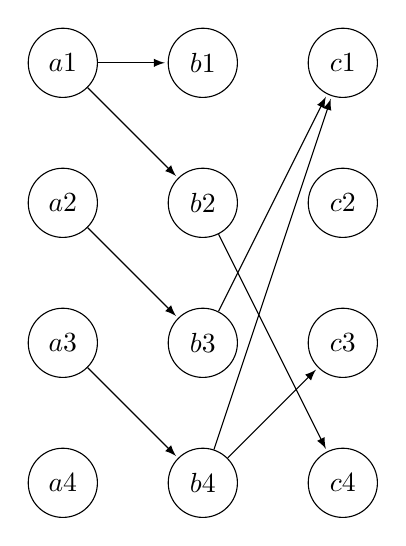
\begin{tikzpicture}[>=latex, shorten >=1pt,node distance=0.7in, on grid, auto]
	\node[state] (a1) {$a1$};
	\node[state] (a2) [below of=a1] {$a2$};
	\node[state] (a3) [below of=a2] {$a3$};
	\node[state] (a4) [below of=a3] {$a4$};
	\node[state] (b1) [right of=a1] {$b1$};
	\node[state] (b2) [below of=b1] {$b2$};
	\node[state] (b3) [below of=b2] {$b3$};
	\node[state] (b4) [below of=b3] {$b4$};
	\node[state] (c1) [right of=b1] {$c1$};
	\node[state] (c2) [below of=c1] {$c2$};
	\node[state] (c3) [below of=c2] {$c3$};
	\node[state] (c4) [below of=c3] {$c4$};
	\path[->]
	(a1) edge node {} (b1)
	(a1) edge node {} (b2)
	(a2) edge node {} (b3)
	(a3) edge node {} (b4)
	(b2) edge node {} (c4)
	(b4) edge node {} (c1)
	(b4) edge node {} (c3)
	(b3) edge node {} (c1)
	;
	\end{tikzpicture}
\end{example}

设$R_1,R_2,R_3$分别是$S$上的二元关系,可以证明以下结论:
\begin{enumerate}
	\item $R_1\circ R_2\ne R_2\circ R_1$。
	\item $(R_1\circ R_2)\circ R_3 = R_1\circ (R_2\circ R_3)$。(结合律)
	\item $(R_1\cup R_2)\circ R_3 = (R_1\circ R_3)\cup(R_2\circ R_3)$。(合成对$\cup$的右分配律)
	\item $R_3\circ(R_1\cup R_2) = (R_3\circ R_1)\cup(R_3\circ R_2)$。(合成对$\cup$的左分配律)
	\item $(R_1\cap R_2)\circ R_3\subseteq(R_1\circ R_3)\cap(R_2\circ R_3)$。(合成对$\cap$的右分配律)
	\item $R_3\circ(R_1\cap R_2)\subseteq(R_3\circ R_1)\cap(R_3\circ R_2)$。(合成对$\cap$的左分配律)
\end{enumerate}

\subsection{递归定义(recurisive definition)与归纳证明}
\begin{itemize}
	\item 递归定义(recurisive definition)
	\begin{itemize}
		\item 又称为归纳定义(indutive definition),它来定义一个集合。
		\item 集合的递归定义由三个部分组成:
		\begin{itemize}
			\item 基础(basis): 用来定义该集合的最基本的元素。
			\item 归纳(induction): 指出用集合中的元素来构造集合的新元素的规则。
			\item 极小性限定: 指出一个对象是所定义集合中的元素的充要条件是它可以通过有限次的使用基础和归纳条款中所给的规定构造出来。
		\end{itemize}
	\end{itemize}
    \item 归纳证明
    \begin{itemize}
    	\item 与递归定义相对应
    	\item 归纳证明方法包括三大步:
    	\begin{itemize}
    		\item 基础(basis): 证明最基本元素具有相应性质。
    		\item 归纳(induction): 证明如果某些元素具有相应性质,则根据这些元素用所规定的方法得到新元素也有相应的性质。
    		\item 根据归纳法原理,所有的元素具有相应的性质。
    	\end{itemize}
    \end{itemize}
\end{itemize}

\begin{example} \label{exr} 算术表达式的递归定义:
	\begin{enumerate}
		\item 基础(basis): 常数是算术表达式,变量是算术表达式;
		\item 归纳(induction): 如果$E_1,E_2$是算术表达式,则$+E_1,-E_1,E_1+E_2,E_1-E_2,E_1\ast E_2,E_1/E_2,E_1\land {E_2},Fun(E_1)$是算术表达式。其中$Fun$为函数名。
		\item 只有满足(1)和(2)的式子才是算术表达式。
	\end{enumerate}
\end{example}

\begin{definition}
	设$R$是$S$上的关系,我们递归地定义$R^n$的幂:
	\begin{enumerate}
		\item $R^0 = \{(a,a)|a\in S\}$
		\item $R^i = R^{i-1}R\quad (i=1,2,3,\cdots)$
	\end{enumerate}
\end{definition}

\begin{example}
对有穷集合$A$, 证明$|2^A| = 2^{|A|}$。
\begin{proof}
	设$A$为一个有穷集合,施归纳于$|A|$:
	\begin{enumerate}
		\item 基础(basis): 当$|A|=0$时,由幂集定义,$|2^A|=|\{\emptyset \}|=1$。而$2^{|A|}=2^0=1$。所以有$|2^A|=2^{|A|}$对$|A|=0$成立。
		\item 归纳(induction): 假设$|A|=n$时结论成立,这里$n\ge 0$,往证当$|A|=n+1$时结论成立。\\
		为此,不妨设$A=B\cup \{a\},a\notin B$,即\\
		$|2^A|=B\cup \{a\}=|B|+|\{a\}|=|B|+1$\\
		由幂集的定义知\\
		$2^A = 2^B \cup \{C\cup \{ a\} | C\in 2^B\}$\\
		由于$a\notin B$,所以\\
		$2^B\cap \{C\cup \{a\}|C\in 2^B \} = \emptyset$\\
		由$\{C\cup \{a\}|C\in 2^B \}$的构造方法知道,可以按如下方法构造一个一一对应的映射$f:\{C\cup \{a\}|C\in 2^B \}\to 2^B$,使\\
		$f(C\cup\{a\})=C$\\
		所以\\
		$|\{C\cup \{a\}|C\in 2^B \}|=|2^B|$\\
		故
		\begin{align*}
			|2^A|&=|2^B \cup \{C\cup \{ a\} | C\in 2^B\}|\\
			&=|2^B|+|\{C\cup \{a\}|C\in 2^B \}| \\
			&=|2^B|+|2^B| \\
			&=2|2^B| 
	    \end{align*}
		显然,$|B|=n$,由归纳假设知\\
		$|2^B|=2^{|B|}$\\
		从而有\\
		$|2^A|=2|2^B|=2\times|2^B|=2^{|B|+1}=2^{|A|}$\\
		这就是说,结论对$|A|=n+1$成立。
		\item 由归纳法原理,结论对任意有穷集合成立。
	\end{enumerate}
\end{proof}	
\end{example}

\begin{example}
	表达式的前缀形式是指将运算符写在前面,后跟相应的运算对象。如:$+E_1$的前缀形式为$+E_1$,$E_1+E_2$的前缀形式为$+E_1E_2$,$E_1\ast E_2$的前缀形式为$\ast E_1E_2$, $E_1\land E_2$的前缀形式为$\land E_1E_2$,$Fun(E_1)$ 的前缀形式为$FunE_1$。
	证明\textit{Example \ref{exr}}所定义的表达式可以用这里定义的前缀形式表示。 	
\end{example}

\begin{proof}
	设$E$为\textit{Example \ref{exr}}所定义的算术表达式,现对$E$中所含的运算符(包括函数引用)的个数实施归纳。设$E$中含$n$个运算符。
	\begin{enumerate}
		\item 基础(basis): 当$n=0$时,表达式为一个常数或者变量,结论显然成立。
		\item 归纳(induction): 假设$n\le k$时结论成立,这里$k\ge 0$,往证当$n=k+1$时结论成立。\\
		由于$E$中含有$k+1$个运算符,所以必须是如下情况中的一种:
		\begin{enumerate}
			\item 当$E=+E_1$时,我们知道$E_1$中的运算符个数为$k$,由归纳假设,$E_1$有对应的前缀形式$F_1$,从而$E$的前缀形式为$+F_1$。
			\item 当$E=-E_1$时,类似地,$E$的前缀形式为$-F_1$。
			\item 当$E=E_1+E_2$时,$E_1,E_2$中的运算符个数分别小于等于$k$,由归纳假设,$E_1,E_2$有对应的前缀形式$F_1,F_2$,从而$E$的前缀形式为$+F_1F_2$。
			\item 对$E=E_1-E_2,E=E_1\ast E_2,E=E_1/E_2,E=E_1\land E_2 $的情况进行类似的讨论,它们的前缀形式分别为: $-F_1F_2,\ast E_1E_2,/E_1E_2,\land E_1E_2$。
			\item 当$E=Fun(E_1)$时,我们知道$E_1$中的运算符个数为$k$,由归纳假设,$E_1$有对应的前缀形式$F_1$,从而$E$的前缀形式为$FunF_1$。
		\end{enumerate}
	    综上所述,结论对$n=k+1$成立。
	    \item 由归纳法原理,结论对\textit{Example \ref{exr}}所定义的所有表达式成立。
	\end{enumerate}
\end{proof}

\subsection{关系的闭包}

\begin{definition}
	设$P$是关于关系的性质的集合,关系$R$的\emph{$P$闭包(closure)}是包含$R$并且具有$P$中所有性质的最小关系。
\end{definition}

\begin{definition}\label{def:R+}
	设$R$是$S$上二元关系,$R$的\emph{正闭包(positive closure)}$R^+$的定义为:
	\subitem(1) $R\subseteq R^{+}$。
	\subitem(2) 如果$(a,b),(b,c) \in R^{+}$,则$(a,c)\in R^{+}$。
	\subitem(3) 除(1)、(2)外,$R^{+}$不包含有其他任何元素。 
    
    可以证明,$R^+$具有传递性,因此又称其为\emph{传递闭包(transitive closure)}。还可以证明,对于任意的二元关系$R$,有
    $$R^{+} = R\cup R^2 \cup R^3 \cup R^4 \cup \dots$$
    且当$S$为有穷集时,有
    \[R^{+} = R\cup R^2 \cup R^3 \cup \cdots \cup R^{|S|} \]
\end{definition}

\begin{definition}\label{def:R*}
	设$R$是$S$上二元关系,$R$的\emph{克林闭包(Kleene closure)}$R^\ast$的定义为:
	\subitem(1) $R^0 \subseteq R^*,R\subseteq R^{\ast}$.
	\subitem(2) 如果$(a,b),(b,c)\in R^{\ast}$则$(a,c)\in R^{\ast}$.
	\subitem(3) 除(1),(2)外,$R^{\ast}$不再含有其他任何元素.
	
	可以证明,$R^\ast$具有自反性和传递性,因此又称其为\emph{自反传递闭包(reflexive and transitive closure)}。
\end{definition}

由定义\ref{def:R+}和\ref{def:R*}可知,对于任意二元关系$R$,有
\begin{align*}
	R^{\ast} &=R^{0}\cup R^{+} \\
	&=R^{0}\cup R\cup R^{2}\cup R^{3}\cup \dots
\end{align*}
而且当$S$为有穷集时:
\[R^{\ast} =R^{0}\cup R\cup R^{2}\cup R^{3}\cup \dots \cup R^{|S|} \]

设$R_1,R_2$是$S$上的两个二元关系,则
\subitem(1) $\emptyset^{+}=\emptyset$
\subitem(2) $(R_1^{+})^{+} = R_1^{+}$
\subitem(3) $(R_1^{\ast})^{\ast} = R_1^{\ast}$
\subitem(4) $R_1^{+}\cup R_2^{+} \subseteq (R_1 \cup R_2)^{+}$
\subitem(5) $R_1^{\ast}\cup R_2^{\ast} \subseteq (R_1\cup R^2)^{\ast}$	

\section{语言}
\subsection{字母表(alphabet)}
\begin{itemize}
	\item \emph{字母表}是一个非空有穷集合,字母表中的元素称为该字母表的一个\emph{字母(letter)}。又叫做\emph{符号(symbol)}、或者\emph{字符(character)}。
	\item 非空性
	\item 有穷性
	\item 字符的两个特性
		\subitem{-} 整体性(monolith), 也叫不可分性
		\subitem{-} 可辨认性(distinguishable),也叫可去区分性
	\item 字母表的乘积(product)
	\[\Sigma_1\Sigma_2 = \{ab|a\in \Sigma_1,b\in \Sigma_2 \} \]
	\item 字母表$\Sigma$的n次幂
		\subitem $\Sigma^0 = \{\epsilon\}$
		\subitem $\Sigma^n = \Sigma^{n-1}\Sigma$
		\subitem $\epsilon$是由$\Sigma$中的0个字符组成的。
	\item $\Sigma$的\emph{正闭包}
		\[\Sigma^{+} = \Sigma \cup \Sigma^2 \cup \Sigma^3 \cup \cdots \]
		\[\Sigma^+ = \{x|x\text{是}\Sigma\text{中的至少一个字符连接而成的字符串}\} \]
	\item $\Sigma$的\emph{克林闭包}
		\[\Sigma^{\ast} = \Sigma^0 \cup \Sigma^+ = \Sigma^0 \cup \Sigma \cup \Sigma^2 \cup \Sigma^3 \cup \cdots \]
		\[\Sigma^{\ast} = \{x|x\text{是}\Sigma\text{中的若干个,包括0个字符,连接而成的字符串}\} \]
\end{itemize}

\begin{example} \{alphabet\}
	\begin{flushleft}
		\{a,b,c,d\}\\
		\{a,b,c,\dots,z\}\\
		\{0,1\} \\
		\{a,$a^{\prime}$,b,$b^{\prime}$ \}\\
		\{aa,ab,bb \}\\
		$\{\infty,\land,\lor,\geq,\leq \}$
	\end{flushleft}
\end{example}

\begin{example} product
	\begin{flushleft}
		\{0,1\}\{0,1\} = \{00,01,10,00\}\\
		\{0,1\}\{a,b,c,d\} = \{0a,0b,0c,0d,1a,1b,1c,1d\}\\
		\{a,b,c,d\}\{0,1\} = \{a0,a1,b0,b1,c0,c1,d0,d1\}\\
		\{aa,ab,bb\}\{0,1\} = \{aa0,aa1,ab0,ab1,bb0,bb1\}
	\end{flushleft}
\end{example}

\begin{example} $\Sigma^0,\Sigma^{\ast}$ 
	\begin{align*}
	\{0,1\}^+ &= \{0,1,00,01,11,000,001,010,011,100,\dots\}\\
	\{0,1\}^{\ast} &= \{\epsilon,0,1,00,01,11,000,001,010,011,100,\dots\}\\
	\{a,b,c,d\}^+ &= \{a,b,c,d,aa,ab,ac,ad,ba,bb,bc,bd,\dots,aaa,aab,aac,aad,aba,abb,abc,\dots\}\\
	\{a,b,c,d\}^{\ast} &= \{\epsilon,a,b,c,d,aa,ab,ac,ad,ba,bb,bc,bd,\dots,aaa,aab,aac,aad,aba,abb,abc,\dots\}
	\end{align*}
\end{example}

\subsection{句子(sentence)/字(word)/字符串(string)}
\begin{itemize}
	\item 别称\\
		句子(sentence),(字符、符号)行(line),(字符、符号)串(string).
	\item 句子(sentence)\\
		$\Sigma$是一个字母表,$\forall \in \Sigma^{\ast},x$叫做$\Sigma$上的一个句子。
	\item 句子相等\\
		两个句子被认为相等的,如果它们对应位置上的字符都对应相等。
	\item 句子的长度(length)
		\subitem{-} $\forall x\in \Sigma^{\ast}$,句子$x$中字符出现的总个数叫做该句子的长度,记作$|x|$。
		\subitem{-} 长度为0的字符串叫\emph{空句子},记作$\epsilon$
	\item 串$x$的$n$次幂
	\begin{align*}
		x^0 &= \epsilon \\
		x^n &= x^{n-1}x
	\end{align*}
\end{itemize}

\begin{note} 注意事项
	\begin{itemize}
		\item $\epsilon$是一个句子
		\item $\{\epsilon\}\ne \emptyset$。这是因为$\{\epsilon\}$不是一个空集,它是含有一个空句子的$\epsilon$的集合。$|\{\epsilon\}|=1,|\emptyset|=0$
	\end{itemize}
\end{note}

\begin{example}
	$$|abaabb|=6$$
	$$|bbaa|=4$$
	$$|\epsilon|=0$$
\end{example}

\begin{example}
	x=001,y=1101
	\begin{align*}
	x^0 &= y^0 = \epsilon \\
	x^4 &= 001001001001 \\
	y^4 &= 1101110111011101
	\end{align*}
\end{example}

\subsection{并置/连结(concatenation)}
\begin{itemize}
	\item 并置/连结(concatenation)
	\subitem{-} $x,y\in \Sigma^{\ast},x,y$的并置是由串$x$直接相接串$y$组成的。记作$xy$.
	\item $\Sigma^{\ast}$上的并置运算性质
	\begin{enumerate}
		\item 结合律: $(xy)z=x(yz)$
		\item 左消去律: if $xy=xz$,then $y=z$
		\item 右消去律: if $yx=zx$,then $y=z$
		\item 惟一分解性: 存在惟一确定的$a_1,a_2,\dots,a_n \in \Sigma$,使得$x=a_1a_2\cdots a_n$.
		\item 单位元素: $\epsilon x=x\epsilon=x$
	\end{enumerate} 
\end{itemize}

\subsection{前缀与后缀}
设$x,y,z,w,v\in \Sigma^{\ast},$且$x=yz,w=yv$
\begin{enumerate}
	\item $y$是$x$的前缀(prefix)
	\item 如果$z\ne \epsilon$,则$y$是x的真前缀(proper prefix).
	\item $z$是$x$的后缀(suffix)
	\item 如果$y\ne \epsilon$,则$z$是$x$的真后缀(proper suffix)
	\item $y$是$x$和$w$的公共前缀(common prefix)
	\item 如果$x$和$w$的任何公共前缀都是$y$的前缀, 则$y$是$x$和$w$的最大公共前缀。
	\item 如果$x=zy$和$w=vy$, 则$y$是$x$和$w$的公共后缀(common suffix)。
	\item 如果$x$和$w$的任何公共后缀都是$y$的后缀, 则$y$是$x$和$w$的最大公共后缀。
\end{enumerate}

\begin{example}
	$\Sigma = \{a,b\}$上的句子abaabb:\\
	前缀: $\epsilon,a,ab,aba,abaa,abaab,abaabb$ \\
	真前缀: $\epsilon,a,ab,aba,abaa,abaab$ \\
	后缀: $\epsilon,b,bb,abb,aabb,baabb,abaabb$ \\
	真后缀: $\epsilon,b,bb,abb,aabb,baabb$
\end{example}

\noindent \textbf{结论}

\begin{enumerate}
	\item $x$的任意前缀$y$有惟一的一个后缀$z$与之对应,使得$x=yz$;反之亦然。
	\item $x$的任意真前缀$y$有惟一的一个真后缀$z$与之对应,使得$x=yz$;反之亦然。
	\item $|\{w|w\text{是}x\text{的后缀}\}| = |\{w|w\text{是}x\text{的前缀}\}|$
	\item $|\{w|w\text{是}x\text{的真后缀}\}| = |\{w|w\text{是}x\text{的真前缀}\}|$
	\item $\{w|w\text{是}x\text{的前缀}\}| = |\{w|w\text{是}x\text{的真前缀}\cup \{x\}\}$
	\item $|\{w|w\text{是}x\text{的前缀}\}| = |\{w|w\text{是}x\text{的真前缀} + 1\}|$
	\item $\{w|w\text{是}x\text{的后缀}\}| = |\{w|w\text{是}x\text{的真后缀}\cup \{x\}\}$
	\item $|\{w|w\text{是}x\text{的后缀}\}| = |\{w|w\text{是}x\text{的真后缀} + 1\}|$
	\item 对于任意字符串$w,w$是自身的前缀,但不是自身的真前缀; $w$是自身的后缀,但不是自身的真后缀。
	\item 对于任意字符串$w,\epsilon$是$w$的前缀,且是$w$的真前缀; $\epsilon$是$w$的后缀,且是$w$的真后缀。
\end{enumerate}

\noindent \textbf{约定}
\begin{itemize}
	\item 用小写字母表中较为靠前的字母$a,b,c,\dots$表示字母表中的字母
	\item 用小写字母表中较为靠后的字母$x,y,z,\dots$表示字母表中的句子(字)
	\item 用$x^T$表示$x$的倒序。例如,如果$x=abc$,则$X^T=cba$
\end{itemize}

\subsection{子串(substring)}
\begin{itemize}
	\item 子串(substring)
		\subitem{-} $w,x,y,z\in \Sigma^{\ast}$,且$w=xyz$,则称$y$是$w$的子串。
	\item 公共子串(common substring)
		\subitem{-} $t,u,v,w,x,y,z\in \Sigma^{\ast}$,且$t=uyv,w=xyz$,则称$y$是$t$和$w$的公共子串(common substring)。如果$y_1,y_2,\dots,y_n$是$t$和$w$的公共子串,且$max\{|y_1|,|y_2|,\dots,|y_n|\}=|y_j|$,则称$y_j$是$t$和$w$的\emph{最大公共子串}。
		\subitem{-} 两个串的最大公共子串并不一定是惟一的。
\end{itemize}

\subsection{语言(language)}
$\forall \in\Sigma^{\ast},L$称为字母表$\Sigma$上的一个\emph{语言(language)},$\forall x\in L,x$叫做$L$的一个句子(sentence)/字(word)/字符串(string)。
\begin{example}
	$\Sigma = \{0,1\}$上的不同语言
	\{00,11\}\\
	\{0,1\}\\
	\{0,1,00,11\}\\
	\{0,1,00,11,01,10\}\\
	\{00,11\}$^{\ast}$\\
	\{01,10\}$^{\ast}$\\
	\{00,01,10,11\}$^{\ast}$\\
	\{0\}\{0,1\}$^{\ast}$\{1\}\\
	\{0,1\}$^{\ast}$\{111\}\{0,1\}$^{\ast}$\\
\end{example}

\subsection{语言的\emph{乘积(product)}}
$L_1\subseteq \Sigma_1^{\ast},L_2\subseteq\Sigma_2^{\ast}$,语言$L_1$与$L_2$的\emph{乘积(product)}是一个语言,该语言定义为:
\[L_1L_2=\{xy|x\in L_1,y\in L_2\}\]
是字母表$\Sigma_1\cup\Sigma_2$上的语言。
\begin{example} $\Sigma = \{0,1\}$
	\begin{align*}
	L_1 &=\{0,1\}\\
	L_2 &=\{00,01,10,11\} \\
	L_3 &=\{0,1,00,01,10,11,000,\dots\} =\Sigma^{+} \\
	L_4 &=\{\epsilon,0,1,00,01,10,11,000,\dots\}=\Sigma^{\ast} \\
	L_5 &=\{0^n|n\geq 1\} \\
	L_6 &=\{0^n1^n\geq 1\} \\
	L_7 &=\{1^n|n\geq 1\} \\
	L_8 &=\{0^n1^m|n,m\geq 1\} \\
	L_9 &=\{0^n1^n0^n|n\geq 1\} \\
	L_{10} &=\{0^n1^m0^k|n,m,k\geq 1\} \\
	L_{11}  &=\{x|x\in\Sigma^{+}\text{且$x$中$0$和$1$的个数相同}\}
	\end{align*}
	\begin{itemize}
		\item 上述所有语言都是$L_4$的子集(子语言);
		\item $L_1,L_2$是有穷语言;其他为无穷语言;其中$L_1$是$\Sigma$上的所有长度为$1$的字组成的语言,$L_2$是$\Sigma$上的所有长度为$2$的字组成的语言;
		\item $L_3,L_4$分别是$\Sigma$的正闭包和克林闭包;
		\item $L_5L_7\ne L_6$,但$L_5L_7=L_8$;同样$L_9\ne L_{10}$,但我们有$L_6\subset L_5L_7, L_9\subset L_{10}$.
		\item $L_6$中的word中的0和1的个数是相同的,并且所有的0在所有的1的前面;$L_{11}$中的word中虽然保持着0和1的个数相同,但它并没有要求所有的0在所有的1的前面。例如,$0101,1100\in L_{11}$,但是$0101\notin L_6$。而对$\forall x\in L_6$,有$x \in L_{11}$。所以$L_6\subset L_{11}$。
	\end{itemize}
\end{example}

\begin{example} $x^T example$
	\begin{enumerate}
		\item $\{x|x=x^T,x\in\Sigma\}$
		\item $\{xx^T|x\in\Sigma^{+}\}$
		\item $\{xx^T|x\in\Sigma^{\ast}\}$
		\item $\{xwx^T|x,w\in\Sigma^{+}\}$
		\item $\{xx^Tw|x,w\in\Sigma^{+}\}$
	\end{enumerate}
\end{example}

\begin{itemize}
	\item 幂
	$\forall L\in\Sigma^{\ast},L$的$n$次\emph{幂}是一个语言,该语言定义为
	\begin{enumerate}
		\item 当$n=0$时,$L^n=\{\epsilon\}$
		\item 当$n\ge 1$时,$L^n=L^{n-1}L$
	\end{enumerate}
	\item 正闭包
	\[L^+=L\cup L^2\cup L^3\cup L^4 \cup\dots\]
	\item 克林闭包
	\[L^{\ast}=L^0\cup L\cup L^2\cup L^3\cup L^4 \cup\dots\]
\end{itemize}

\section{Exercise and Solution}

\begin{exercise}\label{Rl_def}
	设$L$是$\Sigma$上的一个语言,$\Sigma^\ast$上的二元关系$R_L$定义为: 对任给的$x,y\in\Sigma^\ast$,如果对于$\forall z\in\Sigma^\ast$,均有$xz\in L$与$yz\in L$同时成立或者同时不成立,则$xR_L y$。请证明$R_L$是$\Sigma^\ast$上的一个等价关系。将$R_L$称为由语言$L$所确定的等价关系。即
	$$xR_Ly\Leftrightarrow(\forall z\in\Sigma^\ast,xz\in L\Leftrightarrow yz\in L)$$
	
	实际上,$R_L$还有另外一个性质:如果对任给的$x,y\in\Sigma^\ast$, 当$xR_Ly$成立时必有$xzR_Lyz$, 对$\forall z\in\Sigma^\ast$都成立。这将被称为$R_L$的“右不变”性,你能证明此性质成立吗?
\end{exercise}

\begin{solution} 分两步证明$R_L$是“右不变”的等价关系。
	\begin{proof}
		\hfill
		\begin{enumerate}
			\item $R_L$是等价关系。
			\begin{itemize}
				\item 自反性:$\forall x\in\Sigma^\ast$, 显然对于$\forall z\in\Sigma^\ast,xz$要么是$L$的字符串, 要么不是$L$的字符串。由$R_L$的定义知,$xR_Lx$
			    \item 对称性:不难看出,$xR_Ly\Leftrightarrow(\forall z\in\Sigma^\ast,xz\in L\Leftrightarrow yz\in L)\Leftrightarrow yR_Lx$
			    \item 传递性:设$xR_Ly,yR_Lz$。\\
			    $\because$ (由$R_L$的定义知)\\
			    $xR_Ly\Leftrightarrow(\forall w\in\Sigma^\ast, xw\in L\Leftrightarrow yw\in L)$\\
			    $yR_Lz\Leftrightarrow(\forall w\in\Sigma^\ast, yw\in L\Leftrightarrow zw\in L)$\\
			    $\therefore$\\
			    $\forall w\in\Sigma^\ast, xw\in L\Leftrightarrow yw\in L$ and $yw\in L\Leftrightarrow zw\in L$\\
			    $\Rightarrow$\\
			    $\forall w\in\Sigma^\ast, xw\in L\Leftrightarrow zw\in L$
		    \end{itemize}
	    	故\\
	    	$xR_Lz$, 即$R_L$是等价关系。
	    	\item $R_L$是右不变的。\\
	    	设$xR_Ly$。由$R_L$的定义,对$\forall w,v\in\Sigma^\ast,xwv\in L\Leftrightarrow ywv\in L$。注意到$v$的任意性,知$xwR_Lyw$\\
	    	所以,$R_L$是右不变的等价关系。
		\end{enumerate}
	\end{proof}
\end{solution}

\begin{exercise}
	设$\{0,1\}^\ast$上的语言$L=\{0^n1^n|n\ge 0\}$, 请给出$\{0,1\}^\ast$的关于$L$所确定的等价关系$R_L$的等价分类。
\end{exercise}

\begin{solution}
	根据\textbf{Exercise \ref{Rl_def}}对$R_L$的定义及其证明,考虑$R_L$对$\{0,1\}^\ast$的等价分类时,主要需根据语言$L$的结构,分析哪些串按照$L$的要求具有相同的特征。
	\begin{enumerate}
		\item 取$0^n1^n,0^m1^m\in L,0^n1^n\epsilon\in L,0^m1^m\epsilon\in L$同时成立,但是,对所有$x\in\{0,1\}^+,0^n1^nx\in L,0^m1^mx\in L$同时不成立,符合$R_L$的定义。所以,$L$中的元素是属于同一类的。即$0^n1^nR_L0^m1^m\Leftrightarrow(0^n1^n\in L\Leftrightarrow 0^m1^m\in L),n,m\ge 0$。		
		
		\item 分析是否还有其他的元素与$L$中的元素属于同一类。根据$L$的结构,一种类型的串不含子串$10$,这种串可以表示成$0^k1^h,k\ne h$; 另一种是含子串$10$($L$的字符串不含这种子串),这种串可以表示成$x10y$。显然,$01\epsilon\in L$,但是$0^k1^h\notin L(k\ne h),x10y\notin L(x,y\in\{0,1\}^\ast)$。根据等价分类的性质,$\{0,1\}^\ast$中的不在$L$中的串与在$L$的串不在同一个等价类中。
		
		\item 考察不含子串10的串。这些串有如下几种形式:
		\begin{enumerate}
			\item $0^n,n\ge 1$。
			\item $1^n,n\ge 1$。
			\item $0^m1^n,m,n\ge 1,\text{且}m>n$。
			\item $0^m1^n,m,n\ge 1,\text{且}m<n$。
		\end{enumerate}
		对于$0^n,n\ge 1$,$1^n$接在它后面时,构成串$0^n1^n$。显然,当$m\ne n$时,$0^n1^n\in L$, 但$0^m1^n\notin L$。所以,$0^n$和$0^m$一定不在同一个等价类中。
		
		类似的讨论可知,对于$0^n,n\ge 1$:\\	
		$0^n$不可能与形如$0^m1^n(m,n\ge 1,\text{且}m<n)$的串在同一等价类中;\\
		$0^n$不可能与含有子串$10$的串在同一等价类中。
		
		下面再考虑形如$0^k$的串和形如$0^m1^n(m,n\ge 1,\text{且}m>n)$是否可能在同一等价类中。
		
		注意到当$m-n=h$时,
		$$0^h1^h\in L,0^m1^n1^h\in L$$
		同时成立,但是当$n\ge 1,x=01^{h+1}$时$(x\ne 1^h)$,
		$$0^hx\in L,0^m1^nx\notin L$$
		成立。所以,对应$h>0$,令
		$$[h]=\{0^m1^n|m-n=h\text{且}n\ge 1\}$$
		[h]中的元素在同一个等价类中,而且所有其他的元素都不在这个等价类中。实际上,当$h=0$时,有
		$$[0] = L$$
		
		\item 形如$1^m$的串和形如$0^m1^n(m,n\ge 1\text{且}m<n)$的串应该在同一等价类中。	事实上,对于$\{0,1\}^\ast$中的任意字符串$x$,
		$$1^mx\notin L,0^m1^nx\notin L(m,n\ge 1\text{且}m<n)$$
		恒成立。所以,这些字符串在同一个等价类中。
		
		\item 所有含子串$10$的串在同一等价类中。事实上,设$y,z$是含子串$10$的串,对于$\{0,1\}^\ast$中的任意字符串$x$,
			$$yx\notin L,zx\notin L(m,n\ge 1\text{且}m<n)$$
		恒成立。所以,这些字符串在同一个等价类中。
		
		\item 形如$1^m$的串和含子串$10$的串应该在同一等价类中。	事实上,设$y$是含有子串$10$的串,对于$\{0,1\}^\ast$中的任意字符串$x$,
		$$1^mx\notin L,yx\notin L(m\ge 1)$$
		恒成立。所以,这些字符串在同一个等价类中。
		\end{enumerate}
	
		综上所述,$R_L$确定的$\{0,1\}^\ast$的等价分类为\\
		$[10] =\{x10y|x,y\in\{0,1\}^*\}\cup\{0^m1^n|n-m\ge 1\}$ \\
		$[0] =\{0^m1^n|n-m=0\}=\{0^n1^n|n\ge 0\}$ \\
		$[1] =\{0^m1^n|n-m=1\}$ \\
		$[2] =\{0^m1^n|n-m=2\}$ \\
		$\vdots$ \\
		$[h] =\{0^m1^n|n-m=h\}$ \\
		$\vdots$ \\
		$\{0\}$ \\
		$\{00\}$ \\
		$\vdots$ \\
		$\{0^n\}$ \\
		$\vdots$ \\
		其中,$n,m$均为非负整数。
\end{solution}

\begin{exercise} 使用归纳法证明:
	
	对字母表$\Sigma$的任意字符串$x,x$的前缀有$|x|+1$个。
\end{exercise}

\begin{solution}
	\begin{proof}
		设$x\in\Sigma^\ast$,现对$x$的长度施归纳。为了叙述方便用$prefix(x)$表示字符串$x$的所有前缀组成的集合。
		
		当$|x|=0$时,有$x=\epsilon$,由字符串的前缀定义知,$prefix(x)=\{x\}$。\\
		$\epsilon$就是$x$的唯一前缀,而
		\begin{align*}
		|prefix(x) &=|\{\epsilon\}| \\
		           &=1  \\
		           &=0+1 \\
		           &=|x|+1 \\
		\end{align*}
		所以,结论对$|x|=0$成立。
		
		设$|x|=n$时结论成立,$n\ge 0$。即

		$|prefix(x)=|x|+1$\\ 
		现在考察$|x|=n+1$的情况。为了叙述方便,不妨设$x=ya$,其中$|y|=n,a\in\Sigma$。由归纳假设,
		
		$|prefix(y)=|y|+1$ 
		
		首先证明$y$的任何前缀都是$x$的前缀。事实上,设
		
		$|prefix(y)|=\{u_1,u_2,\cdots,u_n\}$	
		
		对于$\forall u\in prefix(y)$,根据前缀的定义,存在$v\in\Sigma^\ast$,使得$uv=y$,注意到$uva=x$,所以,$u$也是$x$的前缀,它对应$x$的后缀为$va$。
		
		再注意到$x=ya$,所以,一方面,对于$\forall u\in prefix(x)$,均有
		
		$u\ne x$\\
		从而
		
		$x\notin prefix(y)$,\\
		然而,由
		
		$x\epsilon=x$\\
		可知,$x$是$x$的一个前缀。另一方面,由$x=ya$知道,如果$u$是$x$的一个前缀,$v$是$u$对应的$x$的后缀,则有如下两种情况:
		\subitem(1) $v\ge 1$,此时必有$u\in prefix(y)$。
		\subitem(2) $|v|=0$,此时必有$v=\epsilon$并且$u=u\epsilon=ya=x$。
		
		\noindent 由此可见,
		\begin{align*}
			prefix(x)&=prefix(y)\cup\{x\} \\
			&=\{u_1,u_2,\cdots,u_n,x\}
		\end{align*}
		由$x\notin prefix(y)$可知,
		\begin{align*}
		|prefix(x)| &= |prefix(y)\cup\{x\}| \\
		&=|prefix(y)|+|\{x\}| \\
		&=|prefix(y)|+1
		\end{align*}
		再由归纳假设,	
		\begin{align*}
			|prefix(x)| &= |prefix(y)|+1 \\
			&=|y|+1+1 \\
			&=|x|+1
		\end{align*}
		
		表明结论对$|x|=n+1$成立。
		
		由归纳法原理,结论对于任意$x\in\Sigma^\ast$成立。$\hfill\square$	
	\end{proof}
    
    \paragraph{另一种往证|x|=n+1时结论成立方法:}
    设$|x|=n$时结论成立,$n\ge 0$。即$|prefix(x)=|x|+1$
     
    现在考察$|x|=n+1$的情况。为了叙述方便,不妨设$x=ya$,其中$|y|=n,a\in\Sigma\& a\ne y$。
    
    $x=ya\Rightarrow$
    \begin{align*}
      prefix(x)&=prefix(ya) &\\
               &=\{\epsilon\}\cup prefix(y) \cup prefix(\{ya\}) &\text{(前缀定义)}\\
               &=\{\epsilon\}\cup prefix(y) \cup prefix(a) & (prefix(\{ya\})=\{\epsilon\}\cup prefix(y)\cup prefix(a)) \\
               &=\{\epsilon\}\cup prefix(y) \cup \{a\} &  (prefix(a)=\{\epsilon,a\})
    \end{align*}
    $\because \epsilon\in prefix(y),a\ne y$,\\
    $\therefore |prefix(x)|= |prefix(y)| + |\{a\}| = |prefix(y)| + 1$\\
    由归纳假设有,$|prefix(y)|=|y|+1$\\
    所以,$|prefix(x)|= |prefix(y)| + 1 = (|y|+1)+1 = |x|+1$\\
    表明结论对$|x|=n+1$成立。
\end{solution}

\begin{exercise}
	设$\Sigma=\{a,b\}$,求字符串$aaaaabbbba$的所有前缀的集合,后缀的集合,真前缀的集合,真后缀的集合。
\end{exercise}

\begin{solution}
	见表(\ref{tab:prepost})。
	
	从表中可以看出,按照前缀与后缀的对应关系构成原来的字符串的对应关系,前缀和后缀是一一对应的,但是,按照这种对应关系,真前缀和真后缀不是一一对应的。不过,若将真后缀和真前缀中的空串$\epsilon$去掉,则这种一一对应关系是仍然存在的。
	
	另外,从对这一问题的讨论知,并不是所有的字符串都有真前缀和真后缀。
	\begin{table}[htbp]
	\caption{$\Sigma=\{a,b\},aaaaabbbba$的前缀,后缀,真前缀,真后缀的集合}
	\label{tab:prepost}
	\begin{tabular}{|c|c|c|c|c|}
		\hline 
		前缀长度&前缀   &是真前缀  &对应后缀      &是真后缀  \\ 
		\hline 
		0&$\epsilon$   &$\surd$  &$aaaaabbbba$ &         \\ 
		\hline 
		1&$a$          &$\surd$  &$aaaabbbba$  &$\surd$  \\ 
		\hline 
		2&$aa$         &$\surd$  &$aaabbbba$   &$\surd$  \\ 
		\hline
	    3&$aaa$        &$\surd$  &$aabbbba$    &$\surd$  \\ 
		\hline
		4&$aaaa$       &$\surd$  &$abbbba$     &$\surd$  \\ 
		\hline
		5&$aaaaa$      &$\surd$  &$bbbba$      &$\surd$  \\
		\hline
		6&$aaaaab$     &$\surd$  &$bbba$       &$\surd$  \\ 
		\hline  
		7&$aaaaabb$    &$\surd$  &$bba$        &$\surd$  \\ 
		\hline
		8&$aaaaabbb$   &$\surd$  &$ba$         &$\surd$  \\ 
		\hline
		9&$aaaaabbbb$  &$\surd$  &$a$          &$\surd$  \\ 
		\hline
		10&$aaaaabbbba$&         &$\epsilon$   &$\surd$  \\ 
		\hline  
	\end{tabular} 
    \end{table}
\end{solution}

\begin{exercise}
	设$L_1,L_2,L_3,L_4$分别是$\Sigma_1,\Sigma_2,\Sigma_3,\Sigma_4$上的语言,能否说$L_1,L_2,L_3,L_4$是某个字母表$\Sigma$上的语言?如果能,请问这个字母表$\Sigma$是什么样的?。
\end{exercise}

\begin{solution}
	可以说$L_1,L_2,L_3,L_4$是同一个字母表$\Sigma$上的语言。这里
	$$\Sigma=\Sigma_1\cup\Sigma_2\cup\Sigma_3\cup\Sigma_4$$
\end{solution}

\begin{exercise}
	设$L_1,L_2,L_3,L_4$分别是$\Sigma_1,\Sigma_2,\Sigma_3,\Sigma_4$上的语言,证明下列等式成立。
	$$(L_1\cup L_2\cup L_3\cup L_4)^\ast=(L_1^\ast L_2^\ast L_3^\ast L_4^\ast)^\ast$$
\end{exercise}

\begin{solution}
	\begin{proof}
		考虑到语言就是一系列字符串的集合,所以,证明两个语言相等,实际上就是证明相应的两个集合相等。因此,为证明
		$$(L_1\cup L_2\cup L_3\cup L_4)^\ast=(L_1^\ast L_2^\ast L_3^\ast L_4^\ast)^\ast$$
		就是证明下列(\ref{eq:1}),(\ref{eq:2})式同时成立。
		\begin{align*}
		(L_1\cup L_2\cup L_3\cup L_4)^\ast &\subseteq(L_1^\ast L_2^\ast L_3^\ast L_4^\ast)^\ast \tag{1}\label{eq:1} \\
		(L_1\cup L_2\cup L_3\cup L_4)^\ast &\supseteq(L_1^\ast L_2^\ast L_3^\ast L_4^\ast)^\ast \tag{2}\label{eq:2}
		\end{align*}
		首先证明(\ref{eq:1})式成立。为此,设
		
		$x\in (L_1\cup L_2\cup L_3\cup L_4)^\ast$\\
		从而存在非负整数$n$和$x_1,x_2,\cdots,x_n,\{x_1,x_2,\cdots,x_n\}\subseteq(L_1\cup L_2\cup L_3\cup L_4)$, 使得
		
		$x=x_1x_2\cdots x_n$\\
		注意到$\{x_1,x_2,\cdots,x_n\}\subseteq(L_1\cup L_2\cup L_3\cup L_4)$,所以,对于$1\le j\le n$
		
		$x_j\in L_1,x_j\in L_2,x_j\in L_3,x_j\in L_4$\\
		中至少一个成立,这表明
		
		$x_j\in L_1^\ast,x_j\in L_2^\ast,x_j\in L_3^\ast,x_j\in L_4^\ast$\\
		中至少一个成立,再注意到
		
		$\epsilon\in L_1^\ast,\epsilon\in L_2^\ast,\epsilon\in L_3^\ast,\epsilon\in L_4^\ast$\\
		并且
		
		$L_1\subseteq L_1^\ast,L_2\subseteq L_2^\ast,L_3\subseteq L_3^\ast,L_4\subseteq L_4^\ast$\\
		使得
		
		$L_1\subseteq L_1^\ast L_2^\ast L_3^\ast L_4^\ast,L_2\subseteq L_1^\ast L_2^\ast L_3^\ast L_4^\ast,L_3\subseteq L_1^\ast L_2^\ast L_3^\ast L_4^\ast,L_4\subseteq L_1^\ast L_2^\ast L_3^\ast L_4^\ast$\\
		从而
		
		$x_j\in  L_1^\ast L_2^\ast L_3^\ast L_4^\ast$\\
		故
		
		$x=x_1x_2\cdots x_n \in  (L_1^\ast L_2^\ast L_3^\ast L_4^\ast)^n$\\
		亦即
		
		$x=x_1x_2\cdots x_n \in  (L_1^\ast L_2^\ast L_3^\ast L_4^\ast)^\ast$\\
		所以(\ref{eq:1})式成立。\\
		类似易证(\ref{eq:2})式亦成立。
		
		综上所述(\ref{eq:1}),(\ref{eq:2})式同时成立。所以,$(L_1\cup L_2\cup L_3\cup L_4)^\ast=(L_1^\ast L_2^\ast L_3^\ast L_4^\ast)^\ast$。$\hfill\square$	
	\end{proof}
\end{solution}

\begin{exercise}
	设$L_1,L_2,L_3,L_4$分别是$\Sigma_1,\Sigma_2,\Sigma_3,\Sigma_4$上的语言,证明下列等式成立否。
	$$L_2(L_1L_2\cup L_2)^\ast L_1=L_1L_1^\ast L_2(L_1L_1^\ast L_2)^\ast$$
\end{exercise}

\begin{solution}
	\begin{proof}
		此式不成立,仅举一个反例即可完成证明。
		
		令 $L_1=\{a\},L_2=\{b\}$,此时,
		
		$L_2(L_1L_2\cup L_2)^\ast L_1=\{b\}(\{a\}\{b\}\cup\{b\})^\ast\{a\}=\{b\}\{ab,b\}^\ast\{a\}$\\
		它含的串都是以$\{b\}开头,以\{a\}结尾的串$。
		
		$L_1L_1^\ast L_2(L_1L_1^\ast L_2)^\ast=\{a\}\{a\}^\ast\{b\}(\{a\}\{a\}^\ast\{b\})^\ast=\{a\}^+\{b\}(\{a\}^+\{b\})^\ast$\\
		它含的串都都是以$\{a\}$开头的串。
		
		所以,此式不成立。$\hfill\square$
	\end{proof}
\end{solution}

\begin{exercise}
	设$\Sigma=\{0,1\}$请给出$\Sigma$上的下列语言的形式化表示。
	\begin{enumerate}
		\item 所有长度为偶数的串。
		\item 所有含有3个连续0的串。
		\item 所有的倒数第10个字符是0的串。
	\end{enumerate}
\end{exercise}

\begin{solution} $\Sigma=\{0,1\}$
	\begin{enumerate}
		\item 所有长度为偶数的串。可以用以下任一种表示方法(含$\epsilon,|\epsilon|=0$,认为是偶数):
		\begin{enumerate}
			\item $(\{0,1\}\{0,1\})^\ast$
			\item $(\{00,01,10,11\})^\ast$
			\item $\{00,01,10,11\}\cup (\{0,1\}\{0,1\})^\ast$
		\end{enumerate}
		\item 所有含有3个连续0的串。\\
		$\{0,1\}^\ast 000\{0,1\}^\ast$
		\item 所有的倒数第10个字符是0的串。\\
		$\{0,1\}^\ast0\{0,1\}\{0,1\}\{0,1\}\{0,1\}\{0,1\}\{0,1\}\{0,1\}\{0,1\}\{0,1\}$
	\end{enumerate}
\end{solution}
 % \cite{蒋宗礼2013}(第1章 绪论)
%\chapter{\cite{蒋宗礼2013}(第3章 有穷状态自动机)}

\emph{主要内容}
\begin{itemize} 
	\item 确定的有穷状态自动机$(DFA)$
		\subitem{-} 作为对实际问题的抽象、直观物理模型、形式定义,DFA接受的句子、语言,状态转移图。
	\item 不确定的有穷状态自动机($NFA$)
		\subitem{-} 定义;
		\subitem{-} NFA与DFA的等价性;
	\item 带空移动的有穷状态自动机($\epsilon-NFA$)
		\subitem{-} 定义。
		\subitem{-} $\epsilon-NFA$与$DFA$的等价性。
	\item $FA$是正则语言的识别器
		\subitem{-} 正则文法($RG$)与$FA$的等价性。
		\subitem{-} 相互转换方法。
		\subitem{-} 带输出的有穷状态自动机。
		\subitem{-} 双向有穷状态自动机。
	\item 重点:$DFA$的概念,$DFA$、$NFA$、$\epsilon-NFA$、$RG$之间的等价转换思路与方法。
	\item 难点:对$DFA$概念的理解,$DFA$、$RG$的构造方法, $RG$与$FA$的等价性证明。
\end{itemize}

\section{语言的识别}

\begin{svgraybox}
	推导和归约中的回溯问题将对系统的效率产生极大的影响 
	
	$S\to aA|aB$
	
	$A\to aA|c$
	
	$B\to aB|d$
	
	分析句子(word)$aaac$的过程中可能需要回溯。
\end{svgraybox}

\begin{itemize}
	\item 识别系统(模型)
	\begin{enumerate}
		\item 系统具有有穷个状态,不同的状态代表不同的意义。按照实际的需要,系统可以在不同的状态下完成规定的任务。
		\item 我们可以将输入字符串中出现的字符汇集在一起构成一个字母表。系统处理的所有字符串都是这个字母表上的字符串。 
		\item 系统在任何一个状态(当前状态)下,从输入字符串中读入一个字符,根据当前状态和读入的这个字符转到新的状态。当前状态和新的状态可以是同一个状态,也可以是不同的状态;当系统从输入字符串中读入一个字符后,它下一次再读时,会读入下一个字符。这就是说,相当于系统维持有一个读写指针,该指针在系统读入一个字符后指向输入串的下一个字符。
		\item 系统中有一个状态,它是系统的开始状态,系统在这个状态下开始进行某个给定句子的处理。 
		\item 系统中还有一些状态表示它到目前为止所读入的字符构成的字符串是语言的一个句子,把所有将系统从开始状态引导到这种状态的字符串放在一起构成一个语言,该语言就是系统所能识别的语言。\item 相应的物理模型
		\begin{enumerate}
			\item 一个右端无穷的输入带。
			\item 一个有穷状态控制器(finite state control,FSC) 。
			\item 一个读头。
		\end{enumerate}
	   \item 系统的每一个动作由三个节拍构成:
	   \begin{enumerate}
	   		\item 读入读头正注视的字符;
	   		\item 根据当前状态和读入的字符改变有穷控制器的状态;
	   		\item 将读头向右移动一格。
	   \end{enumerate}    	
	\end{enumerate}
\end{itemize}

系统识别语言$\{a^nc|n\ge 1\}\cup\{a^nd|n\ge 1\}$的字符串中状态的变化(figure \ref{fig:anc})
\begin{figure}[htbp]
	\includegraphics*[scale=.4]{anc}
	\caption{系统识别语言$\{a^nc|n\ge 1\}\cup\{a^nd|n\ge 1\}$的字符串中状态的变化}
	\label{fig:anc}       % Give a unique label
\end{figure}

有穷状态自动机的物理模型
\begin{figure}[htbp]
	\includegraphics*[scale=.4]{model}
	\caption{有穷状态自动机的物理模型}
	\label{fig:model}       % Give a unique label
\end{figure}

\section{有穷状态自动机(finite automaton,FA)}
\[M=(Q,\Sigma,\delta,q_0,F)\]

$Q$: 状态的非空有穷集合。$\forall\in Q,q$称为$M$的一个\emph{状态(state)}。

$\Sigma$: \emph{输入字母表(Input alphabet)}。输入字符串都是$\Sigma$上的字符串。

$q_0$: $q_0\in Q$,是$M$的\emph{开始状态(initial state)},也可叫做初始状态或者启动状态。

$\delta$: 状态\emph{转移函数(transition function)},有时候又叫做状态转换函数或者移动函数。$\delta: Q\times\Sigma\to Q$,对$\forall(q,a)\in Q\times\Sigma,\delta(q,a)=p$表示:$M$在状态$q$读入字符$a$,将状态变成$p$,并将读头向右移动一个带方格而指向输入字符串的下一个字符。

$F$: $F\subseteq Q$,是$M$的\emph{终止状态(final state)}集合。$\forall q\in F, q$称为$M$的终止状态,又称为\emph{接受状态(accept state)}。  

将$\delta$扩充为
\[\hat{\delta}: Q\times\Sigma^{\ast}\to Q\]

对于任意的$q\in Q, w\in\Sigma^{\ast}, a\in\Sigma$,定义
\begin{enumerate}
	\item $\hat{\delta}(q,\epsilon) = q$
	\item $\hat{\delta}(q,wa) = \delta(\hat{\delta}(q,w),a)$
\end{enumerate}
\begin{align*}
 \hat{\delta}(q,a) &= \hat{\delta}(q,\epsilon a) \\
 				   &= \delta(\hat{\delta}(q,\epsilon),a) \\
 				   &= \delta(q,a)
\end{align*}

两值相同,不用区分这两个符号。 

\paragraph{\textbf{确定的有穷状态自动机}}

由于对于任意的$q\in Q, a\in\Sigma, \delta(q,a)$均有确定的值,所以,将这种FA称为\emph{确定的有穷状态自动机(deterministic finite automaton,DFA) }

\paragraph{\textbf{$M$接受(识别)的语言}}

对于$\forall x\in\Sigma^{\ast}$如果$\delta(q,w)\in F$,则称$x$被$M$接受,如果$\delta(q,w)\notin F$, 则称$M$不接受$x$。
\[L(M)=\{x|x\in\Sigma^{\ast},\text{且}\delta(q,w)\in F\}\]

称为由$M$接受(识别)的语言 

\[L(M_1)=L(M_2)=\{2^{2^n}|n\ge 1\}\]

如果$L(M_1)=L(M_2)$,则称$M_1$与$M_2$等价。

\begin{example}构造一个$DFA$,它接受的语言为
	\[\{x000y|x,y\in\{0,1\}^{\ast}\}\]
	\begin{itemize}
		\item $q_0$: $M$的启动状态;
	    \item $q_1$: $M$读到了一个0,这个0可能是子串“000”的第1个0;
	    \item $q_2$: $M$在$q_1$后紧接着又读到了一个0,这个0可能是子串“000”的第2个0;
		\item $q_3$: $M$在$q_2$后紧接着又读到了一个0,发现输入字符串含有子串“000”;因此,这个状态应该是终止状态。
	    \item $\delta(q_0,1)= q_0$: $M$在$q_0$读到了一个1,它需要继续在$q_0$ “等待”可能是子串“000”的第1个0的输入字符0;
		\item $\delta(q_1,1)= q_0$: $M$在刚刚读到了一个0后,读到了一个1,表明在读入这个1之前所读入的0并不是子串“000”的第1个0,因此,$M$需要重新回到状态$q_0$,以寻找子串“000”的第1个0;
		
		\item $\delta(q_2,1)= q_0$: $M$在刚刚发现了00后,读到了一个1,表明在读入这个1之前所读入的00并不是子串“000”的前两个0,因此,M需要重新回到状态$q_0$,以寻找子串“000”的第1个0;
		
		\item $\delta(q_3,0)= q_3$: $M$找到了子串“000”,只用读入该串的剩余部分。
		
		\item $\delta(q_3,1)= q_3$: $M$找到了子串“000”,只用读入该串的剩余部分。	
	\end{itemize}
	\begin{align*} 
	M=&(\{q_0,q_1,q_2,q_3\},\{0,1\},\\
	&\{\delta(q_0,0)=q_1,\delta(q_1,0)=q_2,\delta(q_2,0)=q_3,\\
	&\delta(q_0,1)=q_0,\delta(q_1,1)=q_0,\delta(q_2,1)=q_0,\\
	&\delta(q_3,0)=q_3,\delta(q_3,1)=q_3\},\\
	&q_0,\{q_3\})
	\end{align*}
	
	see: figure(\ref{fig:x000y}),table(\ref{tab:x000y})
	\begin{table}
		\caption{状态转移表}
		\label{tab:x000y}       % Give a unique label
		\begin{tabular}{|p{1.3cm}|p{0.7cm}|p{0.7cm}|p{0.7cm}|}
		%\begin{tabular}{|c|c|c|c|}
			\hline 
			状态说明 & 状态 & \multicolumn{2}{c|}{输入字符} \\ 
			\hline 
			&  & 0 & 1 \\ 
			\hline 
			开始状态 & $q_0$ & $q_1$ & $q_0$ \\ 
			\hline 
			& $q_1$ & $q_2$ & $q_0$ \\ 
			\hline 
			& $q_2$ & $q_3$ & $q_0$ \\ 
			\hline 
			终止状态 & $q_3$ & $q_3$ & $q_3$ \\ 
			\hline 
		\end{tabular} 
    \end{table}
    \begin{figure}[htbp]
    	\includegraphics*[scale=.4]{x000y}
    	\caption{识别语言\{$x000y|x,y\in\{0,1\}^{\ast}$\}的$DFA$}
    	\label{fig:x000y}       % Give a unique label
    \end{figure}
\end{example}

\begin{example}构造一个$DFA$,它接受的语言为
	\[\{x000|x\in\{0,1\}^{\ast}\}\]
	
	see: figure(\ref{fig:x000})
	\begin{figure}[htbp]
		\includegraphics*[scale=.4]{x000}
		\caption{识别语言\{$x000|x\in\{0,1\}^{\ast}$\}的$DFA$}
		\label{fig:x000}       % Give a unique label
	\end{figure}
\end{example}

\paragraph{}
\begin{note}\emph{几点值得注意}
	\begin{enumerate}
		\item 定义$FA$时,常常只给出$FA$相应的状态转移图就可以了。 
		\item 对于$DFA$来说,并行的弧按其上的标记字符的个数计算,对于每个顶点来说,它的出度恰好等于输入字母表中所含的字符的个数。 
		\item 不难看出,字符串$x$被$FA\quad M$接受的充分必要条件是,在$M$的状态转移图中存在一条从开始状态到某一个终止状态的有向路,该有向路上从第1条边到最后一条边的标记依次并置而构成的字符串$x$。简称此路的标记为$x$。 
		\item 一个$FA$可以有多于1个的终止状态。 
	\end{enumerate}
\end{note}

\paragraph{\textbf{即时描述(instantaneous description,ID)}}

\begin{itemize}
	\item $x,y\in \Sigma^{\ast}, \delta(q_0,x)=q, xqy$称为$M$的一个即时描述,表示$xy$是$M$正在处理的一个字符串,$x$引导$M$从$q_0$启动并到达状态$q$,$M$当前正注视着$y$的首字符。 
	
	\item 如果$xqay$是$M$的一个即时描述,且$\delta(q,a)=p$, 则$xqay\vdash_Mxapy$。
	
	\item $\alpha\vdash_{M^n}\beta$: 表示$M$从即时描述$\alpha$经过$n$次移动到达即时描述$\beta$。
	
	\item $M$存在即时描述$\alpha_1,\alpha_2,\alpha_{n-1}$,使得
	\[\alpha\vdash_M\alpha_1,\alpha_1\vdash_M\alpha_2,\cdots,\alpha_{n-1}\vdash_M\beta\]
	\subitem 当$n=0$时,有$\alpha=\beta$, 即$\alpha\vdash_{M^0}\alpha$
	
	\item $\alpha\vdash_{M^+}\beta$: 表示$M$从即时描述$\alpha$经过至少1次移动到达即时描述$\beta$。
	
	\item $\alpha\vdash_{M^{\ast}}\beta$: 表示$M$从即时描述$\alpha$经过若干步移动到达即时描述$\beta$。
	
	\item 当意义清楚时,我们将符号$\vdash_M, \vdash_{M^n}, \vdash_{M^{\ast}}, \vdash_{M^+}$中的$M$省去,分别用$\vdash, \vdash_n, \vdash_\ast, \vdash_+$表示。	
\end{itemize}

\begin{example}
	图(\ref{fig:x000ID})的DFA到即时描述(instantaneous description,ID)的转换
	\begin{align*}
		q_0101010001 &\vdash 1 q_0 010010001 \\
		&\vdash 10 q_1 10010001 \\
		&\vdash 101 q_0 0010001 \\
		&\vdash 1010 q_1 010001 \\
		&\vdash 10100 q_2 10001 \\
		&\vdash 101001 q_0 0001 \\
		&\vdash 1010010 q_1 001 \\
		&\vdash 10100100 q_2 01 \\
		&\vdash 101001000 q_3 1 \\
		&\vdash 1010010001 q_0
	\end{align*}
	即
	\begin{align*}
		q_0101010001 &\vdash_{10}1010010001 q_0 \\
		q_0101010001 &\vdash_{+}1010010001 q_0 \\
		q_0101010001 &\vdash_{\ast}1010010001 q_0 
	\end{align*}
	对于$x\in\Sigma^{\ast}$,
	\begin{align*}
	q_0x1 &\vdash_{+}x1q_0     \\
	q_0x10 &\vdash_{+}x10q_1   \\
	q_0x100 &\vdash_{+}x100q_2 \\
	q_0x000 &\vdash_{+}x000q_3 
	\end{align*}
	
	\begin{figure}[htbp]
		\includegraphics*[scale=.4]{x000}
		\caption{识别语言\{$x000|x\in\{0,1\}^{\ast}$\}的$DFA$}
		\label{fig:x000ID}       % Give a unique label
	\end{figure}
\end{example}

能引导$FA$从开始状态$q_0$到达$q$的字符串的集合为:
\[set(q)=\{x|x\in\Sigma^{\ast},\delta(q_0,x)=q\}\]

\begin{example}
	对图\ref{fig:x000ID}所给的$DFA$中的所有$q$,求$set(q)$。
	\begin{align*}
		set(q_0) &=\{x|x\in\Sigma^{\ast},x=\epsilon\text{或者$x$以1结尾}\} \\
		set(q_1) &=\{x|x\in\Sigma^{\ast},x=0\text{或者$x$以10结尾}\} \\
		set(q_2) &=\{x|x\in\Sigma^{\ast},x=00\text{或者$x$以100结尾}\} \\
		set(q_3) &=\{x|x\in\Sigma^{\ast},\text{$x$以000结尾}\} \\
		set(q_4) &=\{x|x\in\Sigma^{\ast},\text{$x$以001结尾}\}
	\end{align*}
	这5个集合是两两互不相交。
\end{example}

对于任意一个$FA,\quad M=(Q,\Sigma,\delta,q_0,F)$ 我们可以按照如下方式定义关系$R_M$:

对$\forall x,y\in\Sigma^{\ast},xR_My \Leftrightarrow \exists q\in Q$,使得$x\in set(q)$和$y\in set(q)$同时成立。

按照这个定义所得到的关系实际上是$\Sigma^{\ast}$上的一个等价关系。利用这个关系,可以将$\Sigma^{\ast}$划分成不多于|Q|个等价类。 

\begin{example}
	构造一个$DFA$,它接受的语言为$\{0^n1^m2^k|n,m,k\ge 1\}$。 
	
	$q_0$: $M$的启动状态;
	
	$q_1$: $M$读到至少一个0,并等待读更多的0;
	
	$q_2$: $M$读到至少一个0后,读到了至少一个1,并等待读更多的1;
	
	$q_3$: $M$读到至少一个0后跟至少一个1后,并且接着读到了至少一个2。 
	\begin{itemize}
		\item 先设计“主体框架” ,见图\ref{fig:0n1m2k_1}
		\item 再补充细节, 见图\ref{fig:0n1m2k_2}
	\end{itemize}
	\begin{figure}[htbp]
		\includegraphics*[scale=.4]{0n1m2k_1}
		\caption{语言$\{0^n1^m2^k|n,m,k\ge 1\}$的主题框架}
		\label{fig:0n1m2k_1}       % Give a unique label
	\end{figure}

	\begin{figure}[htbp]
		\includegraphics*[scale=.4]{0n1m2k_2}
		\caption{语言$\{0^n1^m2^k|n,m,k\ge 1\}$的细节}
		\label{fig:0n1m2k_2}       % Give a unique label
	\end{figure}
\end{example}

\begin{enumerate}
	\item 当$FA$一旦进入状态$q_t$,它就无法离开此状态。所以,$q_t$相当于一个陷阱状态(trap)。一般地,我们将陷阱状态用作在其他状态下发现输入串不可能是该$FA$所识别的语言的句子时进入的状态。在此状态下,$FA$读完输入串中剩余的字符。 
	\item  在构造一个识别给定语言的$FA$时,用画图的方式比较方便、直观。我们可以先根据语言的主要特征画出该$FA$的“主体框架”,然后再去考虑画出一些细节要求的内容。
	\item $FA$的状态具有一定的记忆功能:不同的状态对应于不同的情况,由于FA只有有穷个状态,所以,在识别一个语言的过程中,如果有无穷种情况需要记忆,我们肯定是无法构造出相应的$FA$的。 	
\end{enumerate}

\begin{example}
	构造一个$DFA$,它接受的语言为$\{x|x\in \{0,1\}^{\ast}, \text{且当把$x$看成二进制数时,$x$模3与0同余}\}$。 
	
	$q_0$: 对应除以3余数为0的$x$组成的等价类;
	
	$q_1$: 对应除以3余数为1的$x$组成的等价类;
	
	$q_2$: 对应除以3余数为2的$x$组成的等价类;
	
	$q_s$: $M$的开始状态。
	
	$q_s$: 在此状态下读入0时,有$x=0$,所以应该进入状态$q_0$;读入1时,有$x=1$,所以应该进入状态$q_1$。即:$\delta(q_s,0)= q_0; δ(q_s,1)= q_1$。
	
	$q_0$: 能引导$M$到达此状态的$x$除以3余0,所以有:$x=3\times n+0$。
	
	读入0时,引导$M$到达下一个状态的字符串为$x_0,x_0=2\times(3\times n+0)=3\times 2\times n+0$。所以,$\delta(q_0,0)= q_0$;
	
	读入1时,$M$到达下一个状态的字符串为$x_1,x_1=2\times(3\times n+0)+1=3\times 2\times n+1$。所以,$\delta(q_0,1)= q_1$;
	
	$q_1$: 能引导$M$到达此状态的$x$除以3余1,所以有:$x=3\times n+1$。
	读入0时,引导$M$到达下一个状态的字符串为$x_0,x_0=2\times(3\times n+1)=3\times 2\times n+2$。所以即:$\delta(q_1,0)= q_2$;
	
	读入1时,引导$M$到达下一个状态的字符串为$x_1,x_1=2\times(3\times n+1)+1=3\times 2\times n+2+1=3\times(2\times n+1)$。所以$(q_1,1)= q_0$。 
	
	$q_2$: 能引导$M$到达此状态的$x$除以3余2,所以:$x=3\times n+2$。
	读入0时,引导$M$到达下一个状态的字符串为$x_0,x_0=2\times (3\times n+2)=3\times 2\times n+4=3\times(2\times n+1)+1$。所以$\delta(q_2,0)= q_1$;
	
	读入1时,引导$M$到达下一个状态的字符串为$x_1,x_1=2\times(3\times n+2)+1=3\times 2\times n+4+1=3\times(2\times n+1)+2$。所以,$\times(q_2,1)= q_2$。
	
	接受的语言$\{x|x\in \{0,1\}^{\ast}, \text{且当把$x$看成二进制数时,$x$模3与0同余}\}$的$DFA$。如图\ref{fig:mod3}。 
	
	\begin{figure}[htbp]
		\includegraphics*[scale=.4]{mod3}
		\caption{接受的语言$\{x|x\in \{0,1\}^{\ast}, \text{且当把$x$看成二进制数时,$x$模3与0同余}\}$的$DFA$}
		\label{fig:mod3}       % Give a unique label
	\end{figure}
\end{example}

\section{正则代换(regular substitution)}

设$\Sigma,\Delta$是两个字母表,映射
$$f:\Sigma \to 2^{\Delta^{\ast}}$$
被称为是从$\Sigma$到$\Delta$的
\textbf{代换}。如果对于$\forall a\in \Sigma,f(a)$是$\Delta$上的$RL$,则称\textbf{$f$为正则代换}。

\begin{itemize}
	\item 现将$f$的定义域扩展到$\Sigma^{\ast}$上:
	\begin{enumerate}
		\item $f(\epsilon) =\{\epsilon\}$
		\item $f(xa)=f(x)f(a)$
	\end{enumerate}
    \item 再将$f$的定义域扩展到$2^{\Delta^{\ast}}$\\
    对于$\forall L\subseteq \Sigma{\ast}$\\
    $f(L) = \bigcup\limits_{x\in L} f(x)$
    \item $f$是正则代换,则
    \begin{enumerate}
    	\item $f(\emptyset)=\emptyset$
    	\item $f(\epsilon)=\epsilon$
    	\item 对于$\forall a\in \Sigma,f(a)$是$\Delta$上的$RE$
    	\item 如果$r,s$是$\Sigma$上的$RE$,则\\
    	$f(r+s)=f(r)+f(s)$\\
    	$f(rs)=f(r)f(s)$\\
    	$f(r^{\ast}={f(r)}^{\ast}$\\
    	是$\Delta$上的$RE$
    \end{enumerate}
\end{itemize}

\begin{example}
	设$\Sigma={0,1},\Delta={a,b},f(0)=a,f(1)=b^{\ast}$, 则
	\begin{align*}
		f(010) &= f(0)f(1)f(0)=ab^{\ast}a\\
		f({11,00})&=f(11)\cup f(00) \\
		          &=f(1)f(1)\cup f(0)f(0)\\
		          &=b^{\ast}b^{\ast}+aa = b^{\ast}+aa \\
		f(L(0^{\ast}(0+1)1^{\ast})) &= L(a^{\ast}(a+b^{\ast}){(b^{\ast})}^{\ast})\\
		&= L(a^{\ast}(a+b^{\ast})b^{\ast})\\
		&= L(a^{\ast}ab^{\ast} + a^{\ast}b^{\ast}b^{\ast})\\
		&= L(a^{\ast}b^{\ast})
	\end{align*}
\end{example}

\begin{theorem}
	设$L$是$\Sigma$上的一个$RL$
	$$f:\Sigma \to 2^{\Delta^{\ast}}$$
	是正则代换,则$f(L)$也是$RL$. \hfill$\square$ 
\end{theorem}
\begin{proof}
	描述工具$RE$
	
	对$r$中运算符的个数$n$施以归纳,证明$f(r)$是表示$f(L)$的$RE$.
	\begin{itemize}
		\item 当$n=0$时, 结论成立。
		\item 当$n\le k$时,定理成立,即当$r$中运算符的个数不大于$k$时:$f(L(r)) = L(f(r))$。
		\item 当$n=k+1$时,
		\begin{enumerate}
			\item $r=r_1 + r_2$
			\begin{align*}
			f(L) &= f(L(r)) \\
			&=f(L(r_1 + r_2))\\
			&=f(L(r_1)\cup L(r_2))  &\qquad  \text{$RE$的定义} \\
			&=f(L(r_1))\cup f(L(r_2)) &\qquad \text{正则代换的定义} \\
			&=L(f(r_1))\cup L(f(r_2)) &\qquad \text{归纳假设} \\
			&=L(f(r_1)+f(r_2)) &\qquad RE\text{的定义} \\
			&=L(f(r_1+r_2)) &\qquad RE\text{的正则代换的定义} \\
			&=L(f(r))
			\end{align*}
			
			\item $r=r_1r_2$
			\begin{align*}
			f(L) &=f(L(r)) \\
			&=f(L(r_1r_2))\\
			&=f(L(r_1)L(r2)) &\qquad \text{$RE$的定义}\\
			&=f(L(r_1))f(L(r_2)) &\qquad \text{正则代换的定义}\\
			&=L(f(r_1))L(f(r_2)) &\qquad \text{归纳假设} \\
			&=L(f(r_1)f(r_2)) &\qquad \text{$RE$的定义}\\
			&=L(f(r_1r_2)) &\qquad \text{$RE$的正则代换的定义}\\
			&=L(f(r_1r_2))
			\end{align*}
			
			\item $r={r_1}^{\ast}$
			\begin{align*}
			f(L) &=f(L(r)) \\
			&=f(L({r_1}^{\ast}))\\
			&=f(L({r_1})^{\ast}) &\qquad \text{$RE$的定义}\\
			&={(f(L({r_1})))}^{\ast} &\qquad \text{正则代换的定义}\\
			&={(L(f(r_1)))}^{\ast} &\qquad \text{归纳假设} \\
			&=L(f(r_1)^{\ast}) &\qquad \text{$RE$的定义}\\
			&=L(f({r_1}^{\ast})) &\qquad \text{$RE$的正则代换的定义}\\
			&=L(f(r))
			\end{align*}
		\end{enumerate}
	\end{itemize}  \hfill$\square$ 
\end{proof}

%%%%%%%%%%%%%%%%%%%%%%%%% referenc.tex %%%%%%%%%%%%%%%%%%%%%%%%%%%%%%
% sample references
% %
% Use this file as a template for your own input.
%
%%%%%%%%%%%%%%%%%%%%%%%% Springer-Verlag %%%%%%%%%%%%%%%%%%%%%%%%%%
%
% BibTeX users please use
% \bibliographystyle{}
% \bibliography{}
%
\biblstarthook{In view of the parallel print and (chapter-wise) online publication of your book at \url{www.springerlink.com} it has been decided that -- as a genreral rule --  references should be sorted chapter-wise and placed at the end of the individual chapters. However, upon agreement with your contact at Springer you may list your references in a single seperate chapter at the end of your book. Deactivate the class option \texttt{sectrefs} and the \texttt{thebibliography} environment will be put out as a chapter of its own.\\\indent
References may be \textit{cited} in the text either by number (preferred) or by author/year.\footnote{Make sure that all references from the list are cited in the text. Those not cited should be moved to a separate \textit{Further Reading} section or chapter.} The reference list should ideally be \textit{sorted} in alphabetical order -- even if reference numbers are used for the their citation in the text. If there are several works by the same author, the following order should be used: 
\begin{enumerate}
\item all works by the author alone, ordered chronologically by year of publication
\item all works by the author with a coauthor, ordered alphabetically by coauthor
\item all works by the author with several coauthors, ordered chronologically by year of publication.
\end{enumerate}
The \textit{styling} of references\footnote{Always use the standard abbreviation of a journal's name according to the ISSN \textit{List of Title Word Abbreviations}, see \url{http://www.issn.org/en/node/344}} depends on the subject of your book:
\begin{itemize}
\item The \textit{two} recommended styles for references in books on \textit{mathematical, physical, statistical and computer sciences} are depicted in ~\cite{science-contrib, science-online, science-mono, science-journal, science-DOI} and ~\cite{phys-online, phys-mono, phys-journal, phys-DOI, phys-contrib}.
\item Examples of the most commonly used reference style in books on \textit{Psychology, Social Sciences} are~\cite{psysoc-mono, psysoc-online,psysoc-journal, psysoc-contrib, psysoc-DOI}.
\item Examples for references in books on \textit{Humanities, Linguistics, Philosophy} are~\cite{humlinphil-journal, humlinphil-contrib, humlinphil-mono, humlinphil-online, humlinphil-DOI}.
\item Examples of the basic Springer style used in publications on a wide range of subjects such as \textit{Computer Science, Economics, Engineering, Geosciences, Life Sciences, Medicine, Biomedicine} are ~\cite{basic-contrib, basic-online, basic-journal, basic-DOI, basic-mono}. 
\end{itemize}
}

\begin{thebibliography}{99.}%
% and use \bibitem to create references.
%
% Use the following syntax and markup for your references if 
% the subject of your book is from the field 
% "Mathematics, Physics, Statistics, Computer Science"
%
% Contribution 
\bibitem{science-contrib} Broy, M.: Software engineering --- from auxiliary to key technologies. In: Broy, M., Dener, E. (eds.) Software Pioneers, pp. 10-13. Springer, Heidelberg (2002)
%
% Online Document
\bibitem{science-online} Dod, J.: Effective substances. In: The Dictionary of Substances and Their Effects. Royal Society of Chemistry (1999) Available via DIALOG. \\
\url{http://www.rsc.org/dose/title of subordinate document. Cited 15 Jan 1999}
%
% Monograph
\bibitem{science-mono} Geddes, K.O., Czapor, S.R., Labahn, G.: Algorithms for Computer Algebra. Kluwer, Boston (1992) 
%
% Journal article
\bibitem{science-journal} Hamburger, C.: Quasimonotonicity, regularity and duality for nonlinear systems of partial differential equations. Ann. Mat. Pura. Appl. \textbf{169}, 321--354 (1995)
%
% Journal article by DOI
\bibitem{science-DOI} Slifka, M.K., Whitton, J.L.: Clinical implications of dysregulated cytokine production. J. Mol. Med. (2000) doi: 10.1007/s001090000086 
%
\bigskip

% Use the following (APS) syntax and markup for your references if 
% the subject of your book is from the field 
% "Mathematics, Physics, Statistics, Computer Science"
%
% Online Document
\bibitem{phys-online} J. Dod, in \textit{The Dictionary of Substances and Their Effects}, Royal Society of Chemistry. (Available via DIALOG, 1999), 
\url{http://www.rsc.org/dose/title of subordinate document. Cited 15 Jan 1999}
%
% Monograph
\bibitem{phys-mono} H. Ibach, H. L\"uth, \textit{Solid-State Physics}, 2nd edn. (Springer, New York, 1996), pp. 45-56 
%
% Journal article
\bibitem{phys-journal} S. Preuss, A. Demchuk Jr., M. Stuke, Appl. Phys. A \textbf{61}
%
% Journal article by DOI
\bibitem{phys-DOI} M.K. Slifka, J.L. Whitton, J. Mol. Med., doi: 10.1007/s001090000086
%
% Contribution 
\bibitem{phys-contrib} S.E. Smith, in \textit{Neuromuscular Junction}, ed. by E. Zaimis. Handbook of Experimental Pharmacology, vol 42 (Springer, Heidelberg, 1976), p. 593
%
\bigskip
%
% Use the following syntax and markup for your references if 
% the subject of your book is from the field 
% "Psychology, Social Sciences"
%
%
% Monograph
\bibitem{psysoc-mono} Calfee, R.~C., \& Valencia, R.~R. (1991). \textit{APA guide to preparing manuscripts for journal publication.} Washington, DC: American Psychological Association.
%
% Online Document
\bibitem{psysoc-online} Dod, J. (1999). Effective substances. In: The dictionary of substances and their effects. Royal Society of Chemistry. Available via DIALOG. \\
\url{http://www.rsc.org/dose/Effective substances.} Cited 15 Jan 1999.
%
% Journal article
\bibitem{psysoc-journal} Harris, M., Karper, E., Stacks, G., Hoffman, D., DeNiro, R., Cruz, P., et al. (2001). Writing labs and the Hollywood connection. \textit{J Film} Writing, 44(3), 213--245.
%
% Contribution 
\bibitem{psysoc-contrib} O'Neil, J.~M., \& Egan, J. (1992). Men's and women's gender role journeys: Metaphor for healing, transition, and transformation. In B.~R. Wainrig (Ed.), \textit{Gender issues across the life cycle} (pp. 107--123). New York: Springer.
%
% Journal article by DOI
\bibitem{psysoc-DOI}Kreger, M., Brindis, C.D., Manuel, D.M., Sassoubre, L. (2007). Lessons learned in systems change initiatives: benchmarks and indicators. \textit{American Journal of Community Psychology}, doi: 10.1007/s10464-007-9108-14.
%
%
% Use the following syntax and markup for your references if 
% the subject of your book is from the field 
% "Humanities, Linguistics, Philosophy"
%
\bigskip
%
% Journal article
\bibitem{humlinphil-journal} Alber John, Daniel C. O'Connell, and Sabine Kowal. 2002. Personal perspective in TV interviews. \textit{Pragmatics} 12:257--271
%
% Contribution 
\bibitem{humlinphil-contrib} Cameron, Deborah. 1997. Theoretical debates in feminist linguistics: Questions of sex and gender. In \textit{Gender and discourse}, ed. Ruth Wodak, 99--119. London: Sage Publications.
%
% Monograph
\bibitem{humlinphil-mono} Cameron, Deborah. 1985. \textit{Feminism and linguistic theory.} New York: St. Martin's Press.
%
% Online Document
\bibitem{humlinphil-online} Dod, Jake. 1999. Effective substances. In: The dictionary of substances and their effects. Royal Society of Chemistry. Available via DIALOG. \\
http://www.rsc.org/dose/title of subordinate document. Cited 15 Jan 1999
%
% Journal article by DOI
\bibitem{humlinphil-DOI} Suleiman, Camelia, Daniel C. O�Connell, and Sabine Kowal. 2002. `If you and I, if we, in this later day, lose that sacred fire...�': Perspective in political interviews. \textit{Journal of Psycholinguistic Research}. doi: 10.1023/A:1015592129296.
%
%
%
\bigskip
%
%
% Use the following syntax and markup for your references if 
% the subject of your book is from the field 
% "Computer Science, Economics, Engineering, Geosciences, Life Sciences"
%
%
% Contribution 
\bibitem{basic-contrib} Brown B, Aaron M (2001) The politics of nature. In: Smith J (ed) The rise of modern genomics, 3rd edn. Wiley, New York 
%
% Online Document
\bibitem{basic-online} Dod J (1999) Effective Substances. In: The dictionary of substances and their effects. Royal Society of Chemistry. Available via DIALOG. \\
\url{http://www.rsc.org/dose/title of subordinate document. Cited 15 Jan 1999}
%
% Journal article by DOI
\bibitem{basic-DOI} Slifka MK, Whitton JL (2000) Clinical implications of dysregulated cytokine production. J Mol Med, doi: 10.1007/s001090000086
%
% Journal article
\bibitem{basic-journal} Smith J, Jones M Jr, Houghton L et al (1999) Future of health insurance. N Engl J Med 965:325--329
%
% Monograph
\bibitem{basic-mono} South J, Blass B (2001) The future of modern genomics. Blackwell, London 
%
\end{thebibliography}



 % \cite{蒋宗礼2013}(第3章 有穷状态自动机)
%\chapter{\cite{蒋宗礼2013}(第4章 正则表达式)}

\emph{主要内容}
\begin{itemize}
	\item 典型$RE$的构造。
	\item 与$RE$等价$FA$的构造方法。
	\item 与$DFA$等价的$RE$的构造。
	\item 重点
		\subitem{-} $RE$的概念。
		\subitem{-} $RE$与$DFA$的等价性。
	\item 难点
	    \subitem{-} $RE$与$DFA$的等价性证明。 
\end{itemize}

\section{RE的形式定义}
\begin{definition}\label{RE_Def} 正则表达式(regular expression,RE)\\
	设$\Sigma$是一个字母表,以递归形式定义正则表达式:
	\begin{enumerate}
		\item $\emptyset$是$\Sigma$上的$RE$,它表示语言$\emptyset$;
		\item $\epsilon$是$\Sigma$上的$RE$,它表示语言$\{\epsilon\}$;
		\item 对于$\forall a\in\Sigma,a$是$\Sigma$上的$RE$,它便是语言$\{a\}$.
		\item 如果$r,s$分别是$\Sigma$上表示语言$R,S$的$RE$,则:
			\subitem $r,s$的“和”$(r+s)$是$\Sigma$上的$RE,(r+s)$表达的语言为$R\cup S$;
			\subitem $r,s$的“乘积”$(rs)$是$\Sigma$上的$RE,(rs)$表达的语言为$RS$;
			\subitem $r$的克林闭包$(r^\ast)$是$\Sigma$上的$RE,(r^\ast)$表达的语言为$R^\ast$;
		\item 只有满足1,2,3,4的才是$\Sigma$上的$RE$.
	\end{enumerate}
\end{definition}

\begin{example} 设$\Sigma=\{0,1\}$
	\begin{itemize}
		\item $0$,表示语言$\{0\}$
		\item $1$,表示语言$\{1\}$
		\item $(0+1)$,表示语言$\{0,1\}$
		\item $(01)$,表示语言$\{01\}$
		\item $(0+1)^\ast$,表示语言$\{0,1\}^\ast$
		\item $(00)(00)^\ast$,表示语言$\{00\}\{00\}^\ast$
		\item $(0+1)^\ast(0+1)(0+1)^\ast$,表示语言$\{0,1\}^+$
		\item $(0+1)^\ast000(0+1)^\ast$,表示$\{0,1\}$上的至少含有3个连续$0$的串组成的语言
		\item $(0+1)^\ast01$,表示所有以$01$结尾的$0,1$字符串组成的语言
		\item $1(0+1)^\ast0$,表示所有以$1$开头,并且以$0$结尾的$0,1$字符串组成的语言
	\end{itemize}
\end{example}

\emph{约定}
\begin{enumerate}
	\item $r$的正闭包$r^+$表示$r$与$(r^\ast)$的乘积以及$(r^\ast)$与$r$的乘积:
	\[r^+ = rr^\ast = r^\ast r\]
	\item 闭包运算的优先级最高,乘运算的优先级次之,加运算$"+"$的优先级最低。
	\item 在意义明确时,$RE\quad r$表示的语言记为$L(r)$,也可以直接地记为$r$。
	\item 加、乘、闭包运算均执行左结合规则。	
\end{enumerate}

\begin{definition}
	设$r,s$是字母表$\Sigma$上的正则表达式,如果$L(r)=L(s)$,则称$r$和$s$\emph{相等(equivalence,也称为等价)}。
\end{definition}

几个基本结论
\begin{enumerate}
	\item 结合律:
		\subitem $(rs)t=r(st)$
		\subitem $(r+s)+t=r+(s+t)$
	\item 分配律:
		\subitem $r(s+t)=rs+rt$
		\subitem $(s+t)r=sr+tr$
	\item 交换律:$r+s=s+r$
	\item 幂等律:$r+r=r$
	\item 加法运算零元素:$r+\emptyset=r$
	\item 乘法运算单位元:$r\epsilon=\epsilon r=r$
	\item 乘法运算零元素:$r\emptyset=\emptyset r=\emptyset$
	\item $L(\emptyset)=\emptyset$
	\item $L(\epsilon)=\{\epsilon\}$
	\item $L(a)=\{a\}, a\in \Sigma$
	\item $L(rs)=L(r)L(s)$
	\item $L(r+s)=L(r)\cup L(s)$
	\item $L(r^\ast)=(L(r))^\ast$
	\item $L(\emptyset^\ast)=\{\epsilon\}$
	\item $L((r+\epsilon)^\ast)=L(r^\ast)$
	\item $L((r^\ast)^\ast)=L(r^\ast)$
	\item $L((r^\ast s^\ast)^\ast)=L((r+s)^\ast)$
	\item 如果$L(r)\subseteq L(s)$,则$r+s=s$
	\item $L(r^n)=(L(r))^n$
	\item $r^n r^m = r^{n+m}$
\end{enumerate}

\begin{definition}
	设$r$是字母表$\Sigma$上的一个正则表达式,$r$的$n$次幂定义为:
	\begin{enumerate}
		\item $r^0=\epsilon$
		\item $r^n=r^{n-1}r,(n\ge 1)$
	\end{enumerate}
\end{definition}

\begin{note}
	一般地,$r+\epsilon\ne r, (rs)^n \ne r^ns^n, rs\ne sr$.
\end{note}

\begin{example} 设$\Sigma = \{0,1\}$\\
	$00$表示语言$\{00\}$;\\
	$(0+1)^\ast 00(0+1)^\ast$表示所有的至少含两个连续$0$的$0,1$串组成的语言;\\
	$(0+1)^\ast 1(0+1)^9$表示所有的倒数第10个字符为$1$的串组成的语言;\\
	$L((0+1)^\ast 011)=\{x|x\text{是以$011$结尾的$0,1
		$串}\}$;\\
	$L(0^+ 1^+ 2^+)=\{0^n 1^m 2^k|m,n,k\ge 1\}$;\\
	$L(0^\ast 1^\ast 2^\ast)=\{0^n 1^m 2^k|m,n,k\ge 0\}$;\\
	$L(1(0+1)^\ast 1+0(0+1)^\ast 0))=\{x|\text{$x$的开头字符与尾字符相同}\}$。
\end{example}

\section{正则表达式RE与FA等价}
\begin{definition}
	正则表达式$r$称为与$FA\quad M$等价,如果$L(r)=L(M)$。
\end{definition}

从开始状态出发,根据状态之间按照转移所确定的后继关系,依次计算出所给$FA$的各个状态$q$对应的$set(q)$,并且最终得到相应的$FA$接受的语言的$RE$表示。 
寻找一种比较“机械”的方法,使得计算机系统能够自动完成$FA$与$RE$之间的转换。 

\begin{figure}[htbp]
	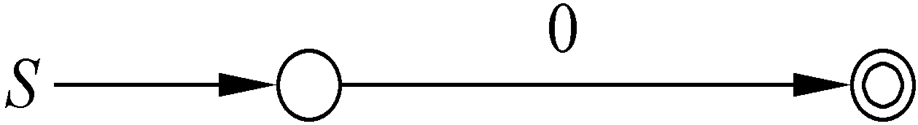
\includegraphics[scale=.4]{0FA}
	\caption{$0$对应的$FA$}
	\label{fig:0FA}       % Give a unique label
\end{figure}

\begin{figure}[htbp]
	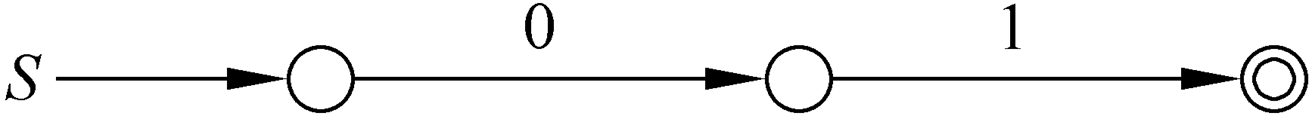
\includegraphics[scale=.4]{01FA}
	\caption{$01$对应的$FA$}
	\label{fig:01FA}       % Give a unique label
\end{figure}

\begin{figure}[htbp]
	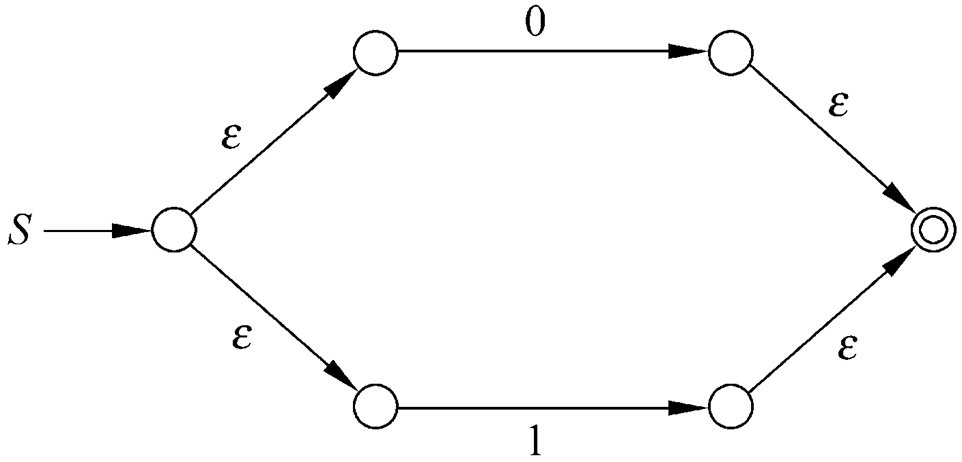
\includegraphics[scale=.4]{0plus1FA}
	\caption{$0+1$对应的$FA$}
	\label{fig:0plus1FA}       % Give a unique label
\end{figure}

\begin{figure}[htbp]
	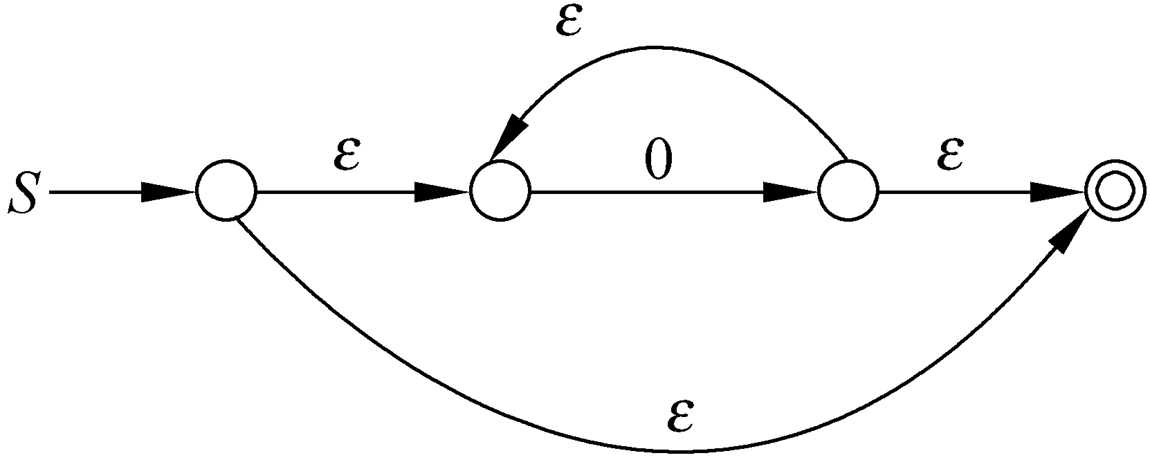
\includegraphics[scale=.4]{0starFA}
	\caption{$0^\ast$对应的$FA$}
	\label{fig:0starFA}       % Give a unique label
\end{figure}

\begin{theorem}
	正则表达式$RE$表示的语言是正则语言$RL$。
\end{theorem}

\begin{proof}
	根据递归表达式的递归定义(\ref{RE_Def}), 施归纳于正则表达式中所含的运算符的个数$n$,证明对于字母表$\Sigma$上的任意正则表达式$r$,存在$FA\quad M$,使得$L(M) = L(r)$ 。
	\begin{itemize}
		\item $M$恰有一个终止状态。
		\item $M$在终止状态下不做移动。
	\end{itemize}

	当$n=0$时,即$r$中不含运算符时,有以下3种情况:
	\begin{enumerate}
		\item $r=\epsilon$,此时图\ref{fig:epsilon_empty_a}(a)所示的$\epsilon -NFA$满足要求。
		\item $r=\emptyset$,此时图\ref{fig:epsilon_empty_a}(b)所示的$\epsilon -NFA$满足要求。
		\item $\forall a\in\Sigma$,此时图\ref{fig:epsilon_empty_a}(c)所示的$\epsilon -NFA$满足要求。
	\end{enumerate}

	所以,结论对$n=0$时成立。
	\begin{figure}[htbp]
		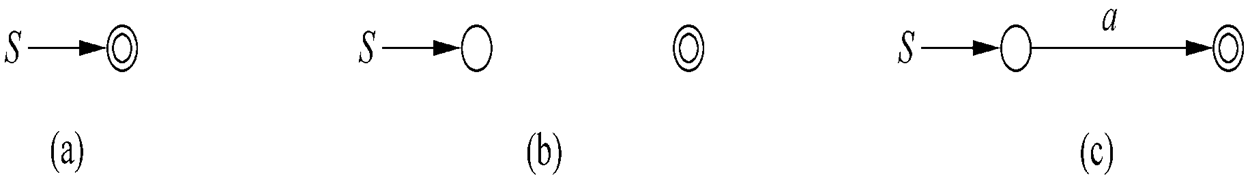
\includegraphics[scale=.45]{epsilon_empty_a}
		\caption{$r=\epsilon,r=\emptyset,r=a$对应的$\epsilon -NFA$}
		\label{fig:epsilon_empty_a}       % Give a unique label
	\end{figure}
    
    假设结论对$n\le k\quad (k\ge 0)$成立,此时有如下$FA$:
    
    $M_1=(Q_1,\Sigma,\delta_1,q_{01},\{f_1\})$
    
    $M_2=(Q_2,\Sigma,\delta_2,q_{02},\{f_2\})$
    
    $L(M_1)=L(r_1), L(M_2)=L(r_2)$
    
    $Q_1\cap Q_2=\emptyset$
    
    \hfill
    
    当$n=k+1$时, $r$有以下3种运算:
    
    \begin{enumerate}
    	\item $r=r_1+r_2$
	    
	    取$q_0,f\notin Q_1\cup Q_2$,令
	    
	    $M=(Q_1\cup Q_2\cup \{q_0,f\},\Sigma,\delta,q_{0},\{f\})$
	    
	    \begin{enumerate}
	    	\item $\delta(q_0,\epsilon)=\{q_{01},q_{02}\}$
	    	\item 对$\forall q\in Q_1,a\in\Sigma\cup\{\epsilon\},\delta(q,a)=\delta_1(q,a)$;\\
	    	对$\forall q\in Q_2,a\in\Sigma\cup\{\epsilon\},\delta(q,a)=\delta_2(q,a)$;
	    	\item $\delta(f_1,\epsilon)=\{f\}$
	    	\item $\delta(f_2,\epsilon)=\{f\}$
	    \end{enumerate}
	    
	    这里构造的$M$,如图(\ref{fig:r_eq_r1_plus_r2})
	    \begin{figure}[htbp]
	    	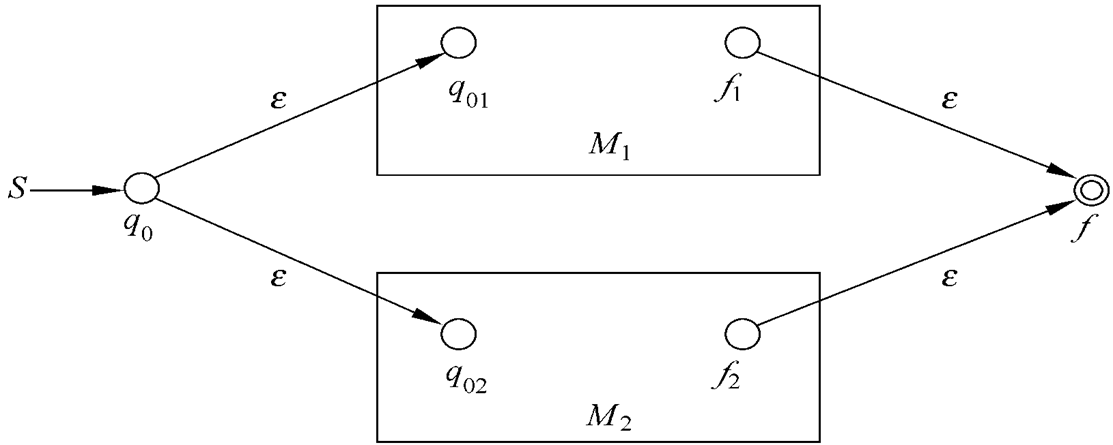
\includegraphics[scale=.45]{r_eq_r1_plus_r2}
	    	\caption{与$r_1+r_2$等价的满足要求的$\epsilon -NFA$}
	    	\label{fig:r_eq_r1_plus_r2}       % Give a unique label
	    \end{figure}
    
        \item $r=r_1r_2$
        
         $M=(Q_1\cup Q_2,\Sigma,\delta,q_{01},\{f_2\})$
        
        \begin{enumerate}
        	\item 对$\forall q\in Q_1-\{f_1\},a\in\Sigma\cup\{\epsilon\},\delta(q,a)=\delta_1(q,a)$;
        	\item 对$\forall q\in Q_2-\{f_2\},a\in\Sigma\cup\{\epsilon\},\delta(q,a)=\delta_2(q,a)$;
        	\item $\delta(f_1,\epsilon)=\{q_{02}\}$
        \end{enumerate}
        
        这里构造的$M$,如图(\ref{fig:r_eq_r1r2})
        \begin{figure}[htbp]
        	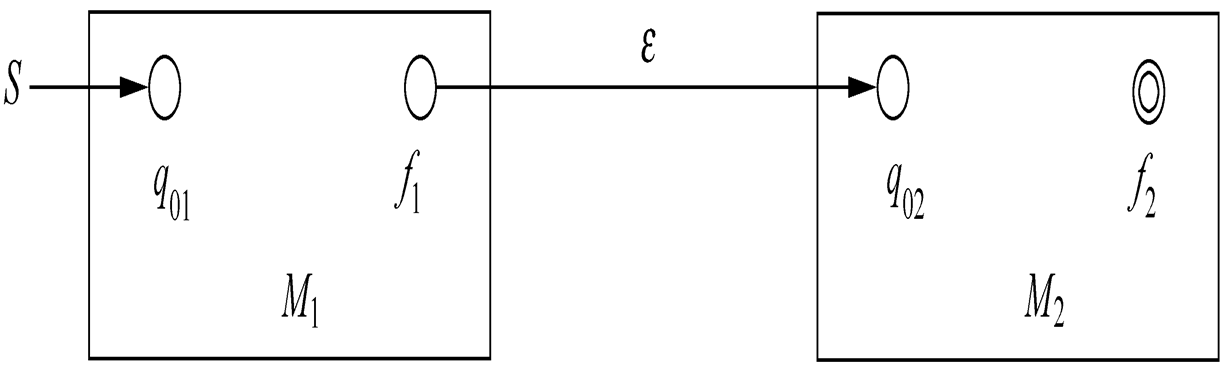
\includegraphics[scale=.45]{r_eq_r1r2}
        	\caption{与$r_1r_2$等价的满足要求的$\epsilon -NFA$}
        	\label{fig:r_eq_r1r2}       % Give a unique label
        \end{figure}
    
	    \item $r=r_1^\ast$
	    
	    $M=(Q_1\cup \{q_0,f\},\Sigma,\delta,q_{0},\{f\})$
	    
	    其中$q_0,f\notin Q_1$, 定义$\delta$为
	    \begin{enumerate}
	    	\item 对$\forall q\in Q_1-\{f_1\},a\in\Sigma,\delta(q,a)=\delta_1(q,a)$;
	    	\item $\delta(f_1,\epsilon)=\{q_{01},f\}$
	    	\item $\delta(q_0,\epsilon)=\{q_{01},f\}$
	    \end{enumerate}
	    
	    这里构造的$M$,如图(\ref{fig:r_eq_r1star})
	    \begin{figure}[htbp]
	    	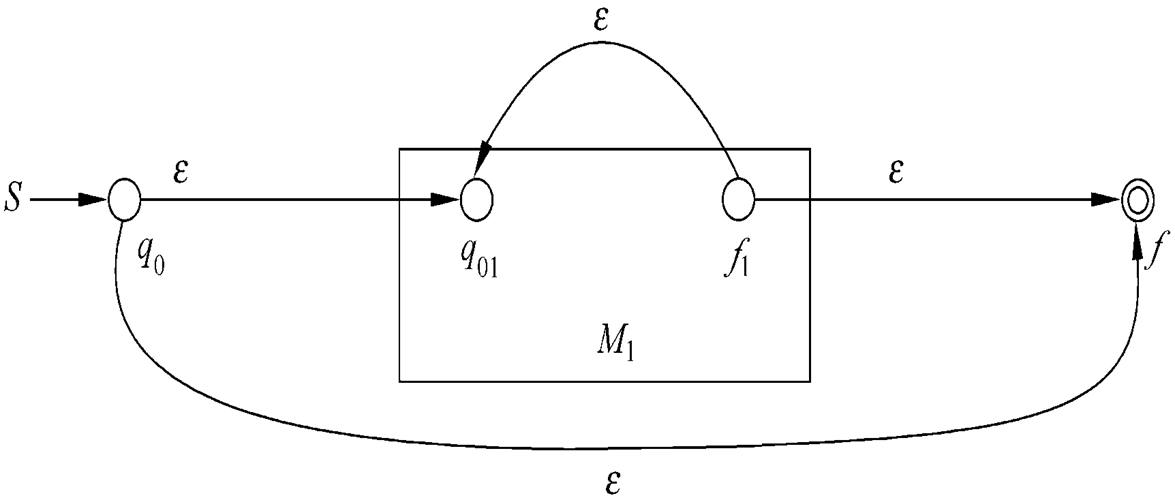
\includegraphics[scale=.45]{r_eq_r1star}
	    	\caption{与$r_1^\ast$等价的满足要求的$\epsilon -NFA$}
	    	\label{fig:r_eq_r1star}       % Give a unique label
	    \end{figure}
	\end{enumerate} 

	因此结论对$n=k+1$成立。由归纳法原理,结论对$\Sigma$上的任意正则表达式成立。
	\hfill$\square$
\end{proof}

\begin{example}
	构造与$(0+1)^\ast 0+(00)^\ast$等价的$FA$。如下图(\ref{fig:ex4-3FA})。  
	\begin{figure}[htbp]
		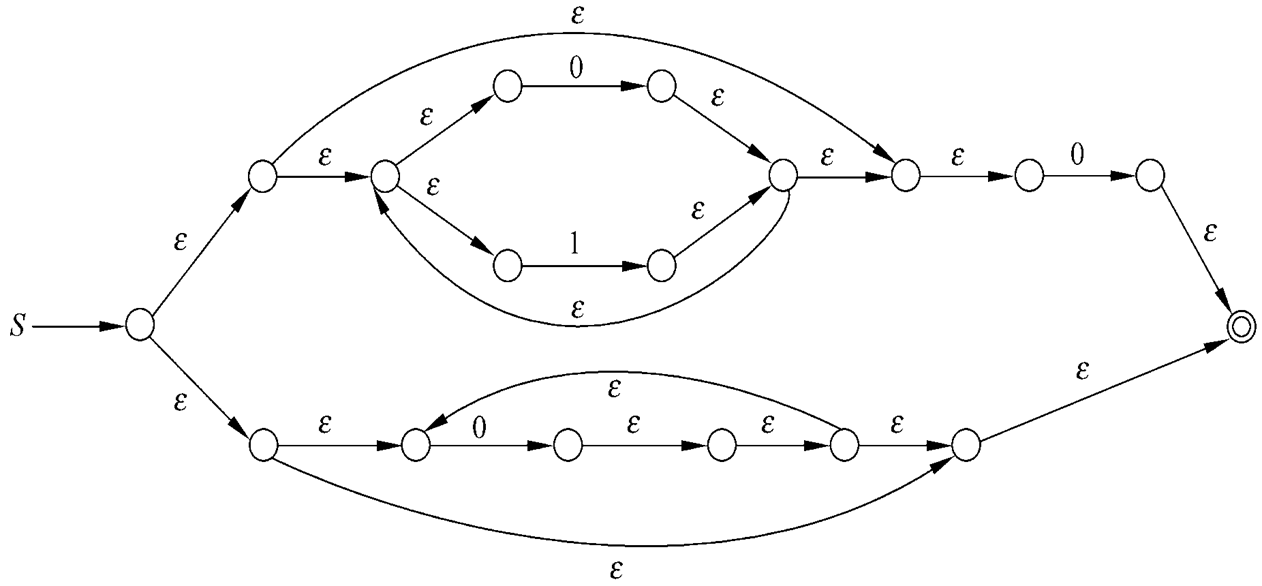
\includegraphics[scale=.45]{ex4-3FA}
		\caption{与$(0+1)^\ast 0+(00)^\ast$等价的$FA$}
		\label{fig:ex4-3FA}       % Give a unique label
	\end{figure}

	按照对$(0+1)^\ast 0+(00)^\ast$的"理解","直接地"构造出的$FA$。
	
	因为,如果$L(r)\subseteq L(s)$,则$r+s=s$, 这里$s=(0+1)^\ast 0,r=(00)^\ast$,因此直接构造出的$FA$如下图(\ref{fig:ex4-3FA1})。 
	\begin{figure}[htbp]
		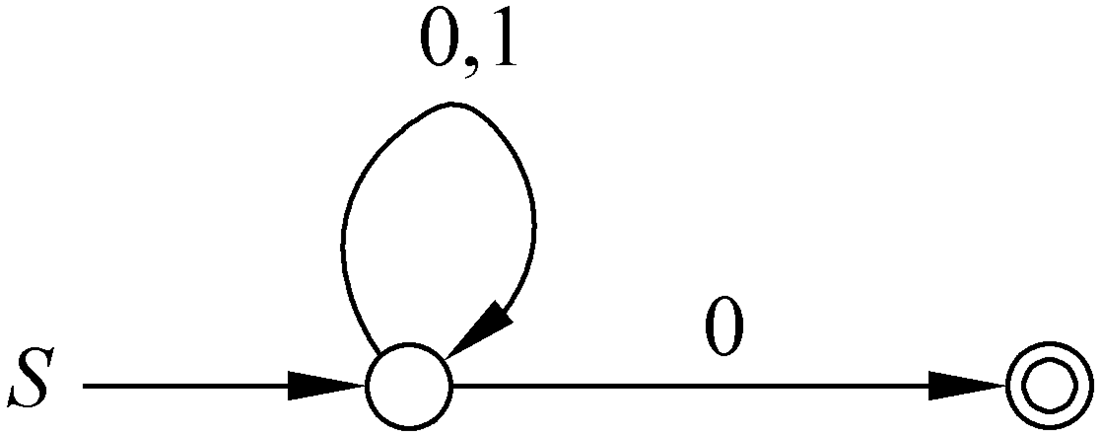
\includegraphics[scale=.45]{ex4-3FA1}
		\caption{与$(0+1)^\ast 0+(00)^\ast$等价的$FA$}
		\label{fig:ex4-3FA1}       % Give a unique label
	\end{figure}
\end{example}

\section{正则语言RL可以用正则表达式RE表示}

\begin{theorem}
	正则语言$RL$可以用正则表达式$RE$表示。
\end{theorem}

设$DFA$
\[M=(\{q_1,q_2,\cdots,q_n\},\Sigma,\delta,q_1,F)\]

令
\[R_{ij}^k = \{x|\delta(q_i,x)=q_j,\text{而且对于$x$的任意前缀$y(y\ne x,y\ne\epsilon)$,如果$\delta(q_i,y)=q_l$,则$l\le k$}\}\]

$R_{ij}^k$表示所有那些将$DFA$从给定状态$q_i$引导到状态$q_j$,并且“途中”不经过(进入并离开)下标大于$k$的状态的所有字符串。值得提醒的是,$i$和$j$的值不受小于等于$k$的限制。

对于$\forall q_i,q_j\in\{q_1,q_2,\cdots,q_n\}, R_{ij}^k$是所有可以将$DFA$从状态$q_i$引导到状态$q_j$的字符串组成的集合。为了便于计算,可以将$R_{ij}^k$递归地定义为:

\[R_{ij}^0 =\begin{cases}
\{a|\delta(q_i,a)=q_j\} &\qquad \text{如果$i\ne j$}\\
\{a|\delta(q_i,a)=q_j\}\cup\{\epsilon\} &\qquad \text{如果$i=j$}
\end{cases}
 \]
 
\[R_{ij}^k = R_{ik}^{k-1}(R_{kk}^{k-1})^\ast R_{kj}^{k-1}\cup R_{ij}^{k-1}\]

显然,
$$L(M)=\bigcup_{q_f\in F}R_{1f}^n$$

当$R_{ij}^0 =\emptyset$时,它对应的正则表达式为$\emptyset$; 当$R_{ij}^0 =\{a_1,a_2,\cdots,a_n\}\ne\emptyset$时,它对应的正则表达式为$a_1+a_2+\cdots+a_n$.

仅当$i=j$时,集合$R_{ij}^0$中含有一个$\epsilon$,而$R_{ij}^k$的表达式中含的都是定义正则表达式时用的运算,所以,容易得到$R_{ij}^k$的正则表达式。

\begin{figure}[htbp]
	\centering
	\begin{minipage}[htbp]{0.3\textwidth}	
	\centerline{} %插入一行,使左右对齐
	\centerline{}
	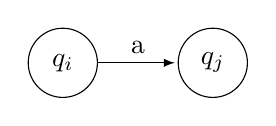
\begin{tikzpicture}[>=latex, shorten >=1pt,node distance=0.75in, on grid, auto]
	% Vertices of automaton
	%\node[state, initial, accepting] (qi) {$q_i$};
	\node[state] (qi) {$q_i$};
	\node[state](qj) [right=of qi] {$q_j$};
	% Edges of automaton
	\path[->] 
	(qi) edge node {a} (qj);
	\end{tikzpicture}
	\centerline{(a) $R_{ij}^0, i\ne j$}
    \end{minipage}
    \begin{minipage}[htbp]{0.3\textwidth}
	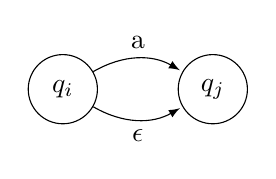
\begin{tikzpicture}[>=latex, shorten >=1pt,node distance=0.75in, on grid, auto]
	% Vertices of automaton
	%\node[state, initial, accepting] (qi) {$q_i$};
	\node[state] (qi) {$q_i$};
	\node[state](qj) [right=of qi] {$q_j$};
	% Edges of automaton
	\path[->] 
	(qi) edge [bend left] node {a} (qj)
	(qi) edge [bend right] node [swap] {$\epsilon$} (qj); 
	\end{tikzpicture}
	\centerline{(b) $R_{ij}^0, i = j$}
    \end{minipage}
    \caption{$R_{ij}^0$对应的$FA$}
    \label{fig:R0-2}       % Give a unique label
\end{figure}

\begin{figure}[htbp]
	\centering
	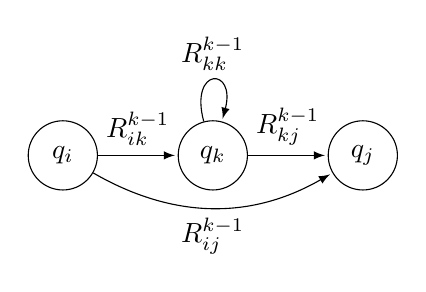
\begin{tikzpicture}[>=latex, shorten >=1pt,node distance=0.75in, on grid, auto]
	% Vertices of automaton
	%\node[state, initial, accepting] (qi) {$q_i$};
	\node[state] (qi) {$q_i$};
	\node[state](qk) [right=of qi] {$q_k$};
	\node[state](qj) [right=of qk] {$q_j$};
	
	% Edges of automaton
	\path[->] 
	(qi) edge node {$R_{ik}^{k-1}$} (qk)
	(qk) edge node {$R_{kj}^{k-1}$} (qj)
	(qk) edge [loop above] node {$R_{kk}^{k-1}$} (qk)
	%(qi) edge [bend right] node {$R_{kj}^{k-1}$} (qj); %弧标记在上
	(qi) edge [bend right] node [swap] {$R_{ij}^{k-1}$} (qj); %弧标记在下
	\end{tikzpicture}
	\caption{$R_{ij}^k$对应的$FA$}
	\label{fig:Rk}       % Give a unique label
\end{figure}


\paragraph{\textbf{图上作业法}}

典型等价变换示例,见图(\ref{fig:figWork})。

\begin{figure}[htbp]
	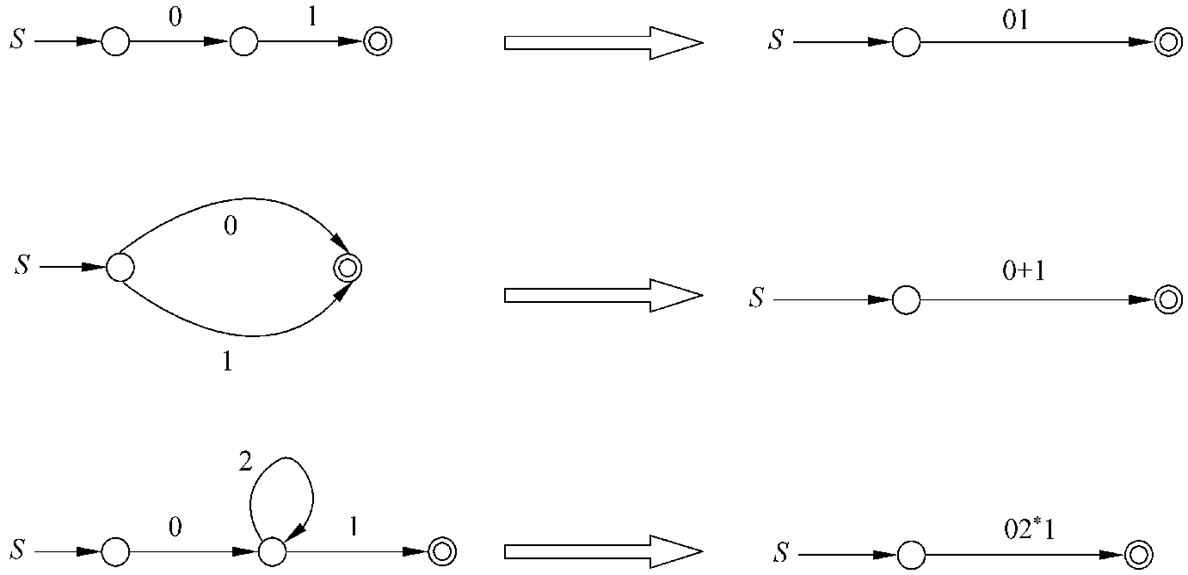
\includegraphics[scale=.45]{figWork}
	\caption{典型等价变换示例}
	\label{fig:figWork}       % Give a unique label
\end{figure}

图上作业法操作步骤
\begin{enumerate}
	\item 预处理:
		\begin{enumerate}
			\item 用标记为$X$和$Y$的状态将$M$“括起来”:
		    \subitem{-} 在状态转移图中增加标记为$X$和$Y$的状态,从标记为$X$的状态到标记为$q_0$的状态引一条标记为$\epsilon$的弧;从标记为$q(q\in F)$的状态到标记为$Y$的状态分别引一条标记为$\epsilon$的弧。
			\item 去掉所有的不可达状态。
		\end{enumerate}
	\item 对通过步骤(1)处理所得到的状态转移图重复如下操作,直到该图中不再包含除了标记为$X$和$Y$外的其他状态,并且这两个状态之间最多只有一条弧。 
		\begin{enumerate}
			\item 并弧
			\subitem{-} 将从$q$到$p$的标记为$r_1,r2,\cdots,r_g$并行弧用从$q$到$p$的、标记为$r_1+r2+\cdots+r_g$的弧取代这$g$个并行弧。 
			\item 去状态1
			\subitem{-} 如果从$q$到$p$有一条标记为$r_1$的弧,从$p$到$t$有一条标记为$r_2$的弧,不存在从状态$p$到状态$p$的弧,将状态$p$和与之关联的这两条弧去掉,用一条从$q$到$t$的标记为$r_1r_2$的弧代替。 
			\item 去状态2
			\subitem{-} 如果从$q$到$p$有一条标记为$r_1$的弧,从$p$到$t$有一条标记为$r_2$的弧,从状态$p$到状态$p$的标记为$r_3$的弧,将状态$p$和与之关联的这三条弧去掉,用一条从$q$到$t$的标记为$r_1r_3^\ast r_2$的弧代替。 
			\item 去状态3
			\subitem{-} 如果图中只有三个状态,而且不存在从标记为$X$的状态到达标记为$Y$的状态的路,则将除标记为$X$的状态和标记为$Y$的状态之外的第3个状态及其相关的弧全部删除。 	
		\end{enumerate}	
	\item 从标记为$X$的状态到标记为$Y$的状态的弧的标记为所求的正则表达式。如果此弧不存在,则所求的正则表达式为$\emptyset$。 	
\end{enumerate}

\begin{example}
	求图(\ref{fig:ex4-4})所示的$DFA$等价的$RE$。
	\begin{figure}[htbp]
		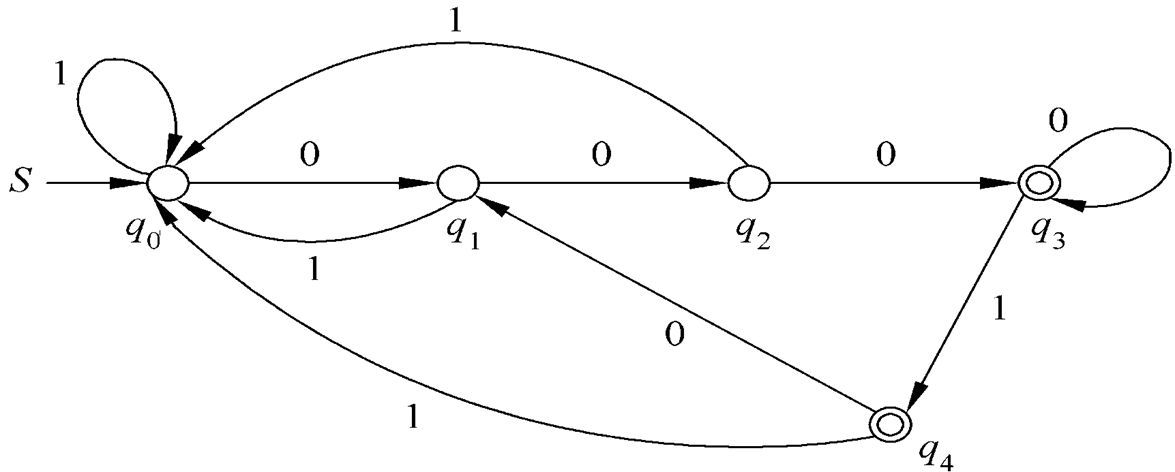
\includegraphics[scale=.45]{ex4-4}
		\caption{由$DFA$构造等价正则表达式的示例$DFA$}
		\label{fig:ex4-4}       % Give a unique label
	\end{figure}
    
    \begin{enumerate}
    	\item 预处理,得到图\ref{fig:ex4-4-1}。
	    \begin{figure}[htbp]
	    	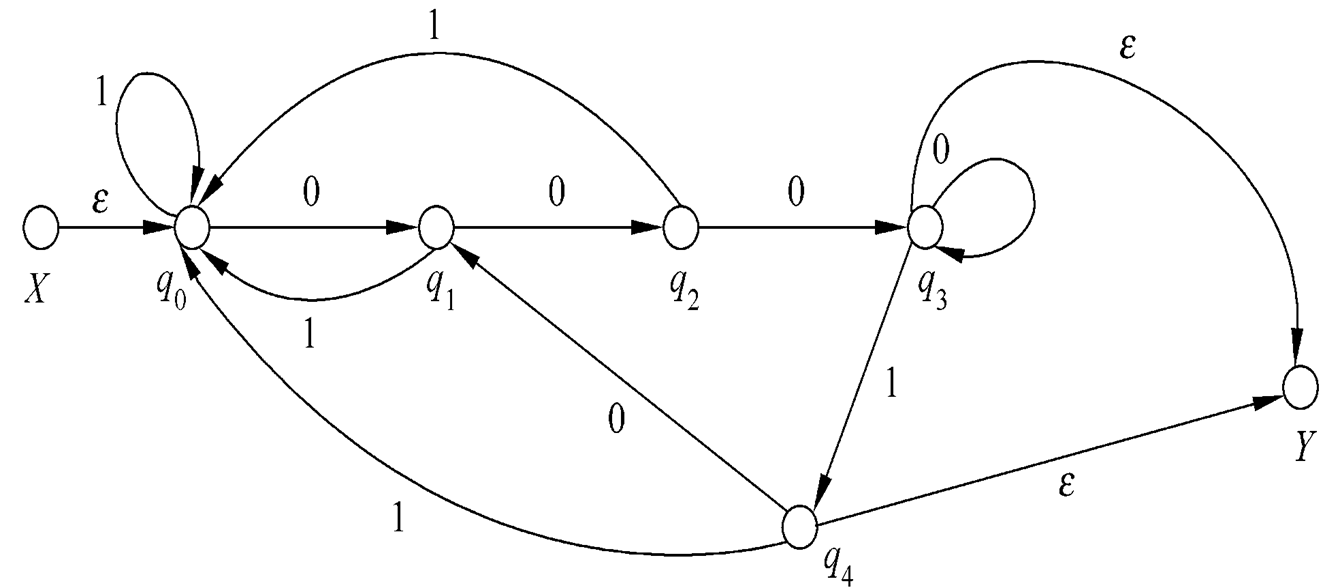
\includegraphics[scale=.45]{ex4-4-1}
	    	\caption{执行步骤(1)后的$DFA$}
	    	\label{fig:ex4-4-1}       % Give a unique label
	    \end{figure}
		\item 去掉状态$q_3$,得到图\ref{fig:ex4-4-2}
		\begin{figure}[htbp]
			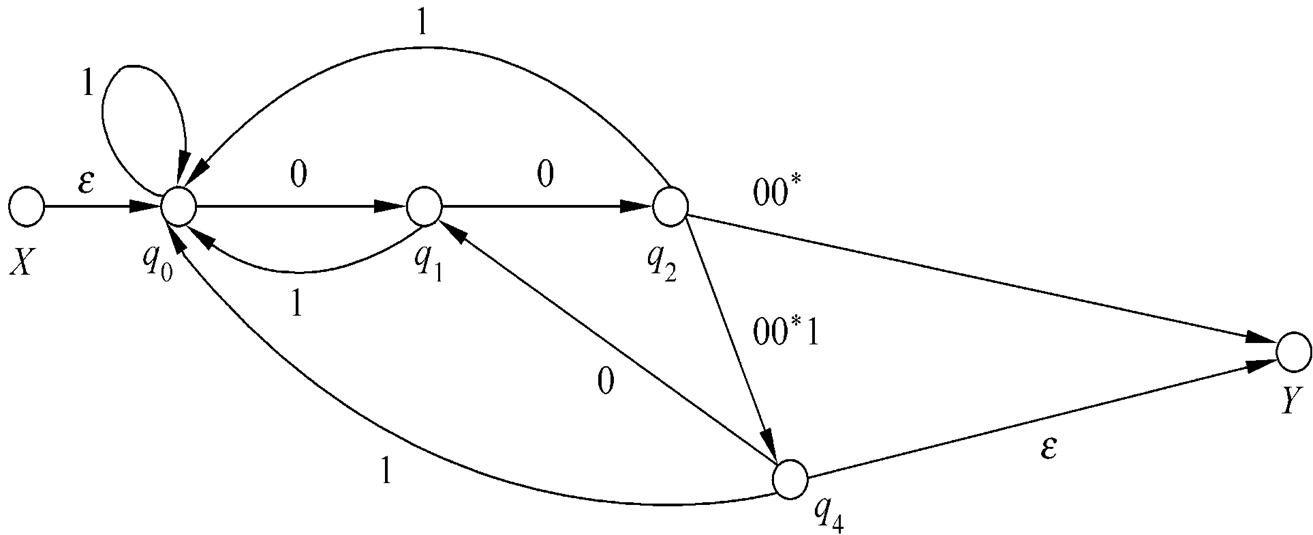
\includegraphics[scale=.45]{ex4-4-2}。
			\caption{去掉状态$q_3$后的$DFA$}
			\label{fig:ex4-4-2}       % Give a unique label
		\end{figure}
	    \item 去掉状态$q_4$,得到图\ref{fig:ex4-4-3}
		\begin{figure}[htbp]
			\includegraphics[scale=.45]{ex4-4-3}
			\caption{去掉状态$q_4$后的$DFA$}
			\label{fig:ex4-4-3}       % Give a unique label
		\end{figure}
	    \item 合并从标记为$q_2$的状态到标记为$Y$的状态的两条并行弧。得到图\ref{fig:ex4-4-4}。 
	    \begin{figure}[htbp]
	    	\includegraphics[scale=.45]{ex4-4-4}
	    	\caption{合并后的$DFA$}
	    	\label{fig:ex4-4-4}       % Give a unique label
	    \end{figure}
        \item 去掉状态$q_0$,得到图\ref{fig:ex4-4-5}。
        \begin{figure}[htbp]
        	\includegraphics[scale=.3]{ex4-4-5}
        	\caption{去掉状态$q_0$后的$DFA$}
        	\label{fig:ex4-4-5}       % Give a unique label
        \end{figure}
        \item 并弧,得到图\ref{fig:ex4-4-6}。
        \begin{figure}[htbp]
        	\includegraphics[scale=.45]{ex4-4-6}
        	\caption{并弧后的$DFA$}
        	\label{fig:ex4-4-6}       % Give a unique label
        \end{figure}
        \item 去掉状态$q_1$,得到图\ref{fig:ex4-4-7}。
        \begin{figure}[htbp]
        	\includegraphics[scale=.45]{ex4-4-7}
        	\caption{去掉状态$q_1$后的$DFA$}
        	\label{fig:ex4-4-7}       % Give a unique label
        \end{figure}\item 去掉状态$q_1$
        \item 去掉状态$q_2$,得到图\ref{fig:ex4-4-8}。
	    \begin{figure}[htbp]
	    \includegraphics[scale=.45]{ex4-4-8}
	    \caption{去掉状态$q_2$后的$DFA$}
	    \label{fig:ex4-4-8}       % Give a unique label
		\end{figure}
	\end{enumerate}

得到以下正则表达式,就是所求。
$$1^\ast 0(11^\ast 0)^\ast 0((00^\ast 111^\ast 0+00^\ast 10+11^\ast 0)(11^\ast 0)^\ast 0)(00^\ast+00^\ast 1)$$ 
\end{example}

\begin{note}
	以下几点需要注意:
	\begin{enumerate}
		\item 如果去状态的顺序不一样,则得到的$RE$可能在形式是不一样,但它们都是等价的。 
		\item 当$DFA$的终止状态都是不可达的时候,状态转移图中\emph{必不存在}从开始状态到终止状态的路。此时,相应的$RE$为$\emptyset$。
		\item 不计算自身到自身的弧,如果状态$q$的入度为$n$,出度为$m$,则将状态$q$及其相关的弧去掉之后,需要添加$n\times m$条新弧。 
		\item 对操作的步数施归纳,可以证明它的正确性。	
	\end{enumerate}
\end{note}

\begin{corollary}
	正则表达式与$FA$、正则文法等价,是正则语言的表示模型。
\end{corollary}

\section{正则语言等价模型的总结}
到此,一共给出了正则语言的5种等价描述模型:正则文法(RG),确定的有穷状态自动机(DFA),不确定的有穷状态自动机(NFA),带空移动的有穷状态自动机($\epsilon -NFA$),正则表达式(RE)。他们之间的等价转换如图(\ref{fig:model_ev})。
\begin{figure}[htbp]
	\includegraphics[scale=.6]{model_ev}
	\caption{正则语言5中等价模型的转换}
	\label{fig:model_ev}       % Give a unique label
\end{figure}

\paragraph{小结}
本章讨论了RL及其与FA的等价性。
\begin{enumerate}
	\item 字母表$\Sigma$上的$RE$用来表示$\Sigma$上的$RL$。$\emptyset,\epsilon,a\in\Sigma$是$\Sigma$上的最基本的$RE$,它们分别表示语言$\emptyset,\{\epsilon\},\{a\}$,以此为基础,如果$r$和$s$分别是$\Sigma$上的表示语言$R$和$S$的$RE$,则$r+s,rs,r^\ast$分别是$\Sigma$上的表示语言$R\cup S,RS,R^\ast$的$RE$。如果$L(r)=L(s)$,则称$r$与$s$等价。  
	\item $RE$对乘、加满足结合律;乘对加满足左、右分配律;加满足交换率和幂等率;$\emptyset$是加运算的零元素;$\epsilon$是乘运算的单位元;$\emptyset$是乘运算的零元素。
	\item $RE$是$RL$的一种描述。容易根据$RE$构造出与它等价的$FA$。反过来,可以用图上作业法构造出与给定的$DFA$等价的$RE$。
	\item $RL$的5种等价描述模型转换图。  
\end{enumerate}

\section{Exercise and Solution}
\begin{exercise}
	写出下列语言的正则表达式。
	\begin{enumerate}
		\item ${0,1}^+$。
		\item $\{x|x\in \{0,1\}^\ast \text{且$x$中不含形如$00$的子串}\}$。
	\end{enumerate}	
\end{exercise}

\begin{solution}
	\hfill
	\begin{enumerate}
	\item ${0,1}^+$\\
		  $r=(0+1)(0+1)^\ast$
	\item $\{x|x\in \{0,1\}^\ast \text{且$x$中不含形如$00$的子串}\}$
		\begin{enumerate}
			\item 分析语言,直接构造正则表达式。\\
			$r_1=(1+01)^\ast=\{x|x\text{无连续的0,但以1结尾;当以0开头时,长度不小于2}\}$ \\
			$r_2=(1+10)^\ast=\{x|x\text{无连续的0,以1开头,但以0或者以1结尾;当以0结尾时,长度不小于2}\}$ \\
			$r_3=(1+01)^\ast 0=\{x|x\text{无连续的0,以0结尾;长度至少为1}\}$ \\	
			$r_4= 0 =\{x|x\text{无连续的0,以0开头和结尾;长度为1}\}$ \\
			$\because r_4\subseteq r_3 \\ \therefore r_3 = r_3+r_4$\\
			$r= r_1+r_2+r_3+r_4 = r_1+r_2+r_3$\\		
			$r=(1+01)^\ast + (1+10)^\ast + (1+01)^\ast 0 =(1+10)^\ast + (1+01)^\ast(\epsilon+0)$\\
			\\
			另一种思路是根据$(1+01)^\ast$和$(1+10)^\ast$直接补充所缺部分。\\
			用$0(1+10)^\ast$补上以0开头的满足要求的字符串:\\
			$(1+10)^\ast + 0(1+10)^\ast=(\epsilon + 0)(1+10)^\ast$\\
			或者用$(1+01)^\ast 0$补上以0结尾的满足要求的字符串:\\
			$(1+01)^\ast + (1+01)^\ast 0=(1+01)^\ast(0+\epsilon)$
			\item 图上作业法。\\
			\begin{tabular}{|c|c|}
				\hline 
				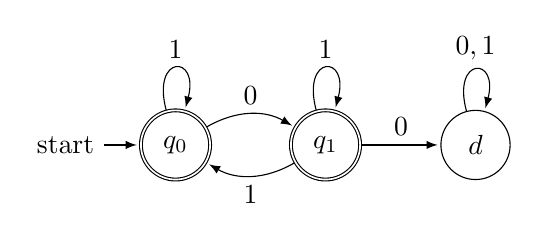
\begin{tikzpicture}[>=latex, shorten >=1pt,node distance=0.75in, on grid, auto]
					\node[state,initial,accepting] (q0) {$q_0$};
					\node[state,accepting](q1) [right=of q0] {$q_1$};
					\node[state](dump) [right=of q1] {$d$};
					\path[->]
					(q0) edge [loop above] node {$1$} (q0) 
					(q0) edge [bend left] node {$0$} (q1)
					(q1) edge [bend left] node {$1$} (q0)
					(q1) edge [loop above] node {$1$} (q1) 
					(q1) edge node {$0$} (dump)
					(dump) edge [loop above] node {$0,1$} (dump);
				\end{tikzpicture} & 
				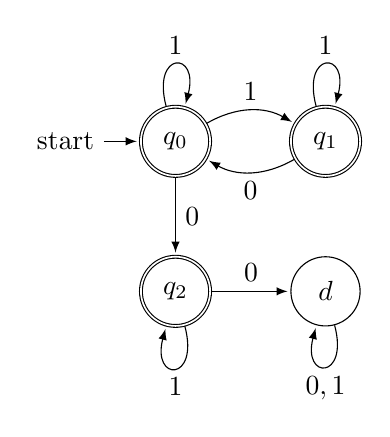
\begin{tikzpicture}[>=latex, shorten >=1pt,node distance=0.75in, on grid, auto]
					\node[state,initial,accepting] (q0) {$q_0$};
					\node[state,accepting](q1) [right=of q0] {$q_1$};
					\node[state,accepting] (q2) [below=of q0] {$q_2$};
					\node[state](dump) [right=of q2] {$d$};
					\path[->]
					(q1) edge [loop above] node {$1$} (q1) 
					(q0) edge [loop above] node {$1$} (q0)
					(q0) edge [bend left] node {$1$} (q1)
					(q1) edge [bend left] node {$0$} (q0)
					(q0) edge node {$0$} (q2)
					(q2) edge [loop below] node {$1$} (q2)
					(q2) edge node {$0$} (dump)
					(dump) edge [loop below] node {$0,1$} (dump);
				\end{tikzpicture} \\
				%\hline 
				(a) NFA: $1^n+(01)^n + 0$ & (b) NFA: $1^n+(10)^n+0$ \\ 
				\hline 
				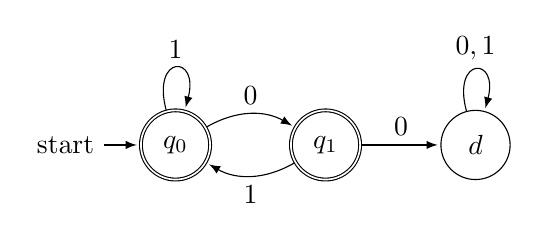
\begin{tikzpicture}[>=latex, shorten >=1pt,node distance=0.75in, on grid, auto]
				\node[state,initial,accepting] (q0) {$q_0$};
				\node[state,accepting](q1) [right=of q0] {$q_1$};
				\node[state](dump) [right=of q1] {$d$};
				\path[->]
				(q0) edge [loop above] node {$1$} (q0) 
				(q0) edge [bend left] node {$0$} (q1)
				(q1) edge [bend left] node {$1$} (q0)
				(q1) edge node {$0$} (dump)
				(dump) edge [loop above] node {$0,1$} (dump);
				\end{tikzpicture} & 
				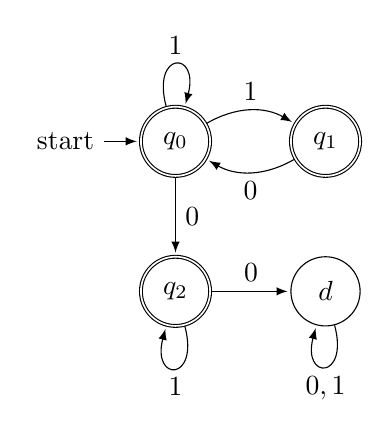
\begin{tikzpicture}[>=latex, shorten >=1pt,node distance=0.75in, on grid, auto]
				\node[state,initial,accepting] (q0) {$q_0$};
				\node[state,accepting](q1) [right=of q0] {$q_1$};
				\node[state,accepting] (q2) [below=of q0] {$q_2$};
				\node[state](dump) [right=of q2] {$d$};
				\path[->]
				(q0) edge [loop above] node {$1$} (q0)
				(q0) edge [bend left] node {$1$} (q1)
				(q1) edge [bend left] node {$0$} (q0)
				(q0) edge node {$0$} (q2)
				(q2) edge [loop below] node {$1$} (q2)
				(q2) edge node {$0$} (dump)
				(dump) edge [loop below] node {$0,1$} (dump);
				\end{tikzpicture} \\
				%\hline 
				(c) DFA: $1^n+(01)^n + 0$ & (d) DFA: $1^n+(10)^n+0$ \\ 
				\hline
				\multicolumn{2}{|c|}
				{
					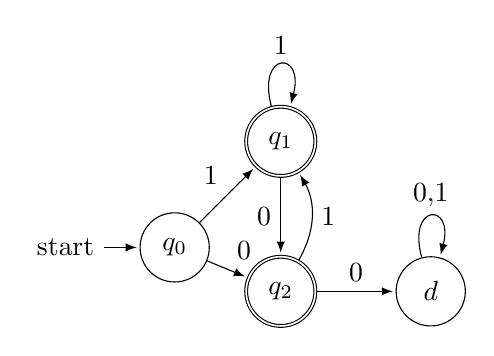
\begin{tikzpicture}[>=latex, shorten >=1pt,node distance=0.75in, on grid, auto]
					\node[state,initial] (q0) {$q_0$};
					\node[state,accepting](q1) [above right=of q0] {$q_1$};
					\node[state,accepting] (q2) [below=of q1] {$q_2$};
					\node[state](dump) [right=of q2] {$d$};
					\path[->]
					(q0) edge node {$1$} (q1)
					(q0) edge node {$0$} (q2)
					(q1) edge [loop above] node {$1$} (q1)
					(q1) edge [swap] node {$0$} (q2)
					(q2) edge [bend right,swap] node {$1$} (q1)
					(q2) edge node {$0$} (dump)
					(dump) edge [loop above] node {0,1} (dump) ;
					\end{tikzpicture} 
				}\\
				%\hline
				\multicolumn{2}{|l|}{构造$\{x|x\in\{0,1\}^+ \text{且$x$中不含形如$00$的子串}\}$语言的$DFA$.}\\ 
				\multicolumn{2}{|l|}{构造要点是,自动机启动并读入一个字符后,就将"精力"集中在考察是否出现$00$子串上,}\\
				\multicolumn{2}{|l|}{一旦发现子串$00$,就进入陷阱状态。}\\
				\hline
			\end{tabular} 
		\end{enumerate}
	\end{enumerate}
\end{solution}

\begin{exercise}
	构造下列正则表达式的等价$FA$。
	$$((0+1)(0+1))^\ast+((0+1)(0+1(0+1))^\ast$$
\end{exercise}

\begin{solution}
	\hfill
	\begin{enumerate}
		\item $(0+1)(0+1))^\ast+((0+1)(0+1(0+1))^\ast$的等价$FA$见图(\ref{fig:0101FA})。
		\item $(0+1)(0+1))^\ast+((0+1)(0+1(0+1))^\ast$的\emph{不等价}$FA$见图(\ref{fig:0101-1FA})。
		\item $(0+1)(0+1))^\ast+((0+1)(0+1(0+1))^\ast$的\emph{不等价}$FA$见图(\ref{fig:0101-2FA})。
		\item $(0+1)(0+1))^\ast+((0+1)(0+1(0+1))^\ast$的\emph{不等价}$FA$见图(\ref{fig:0101-3FA})。
	\end{enumerate}
	\begin{figure}[htbp]
		\centering
		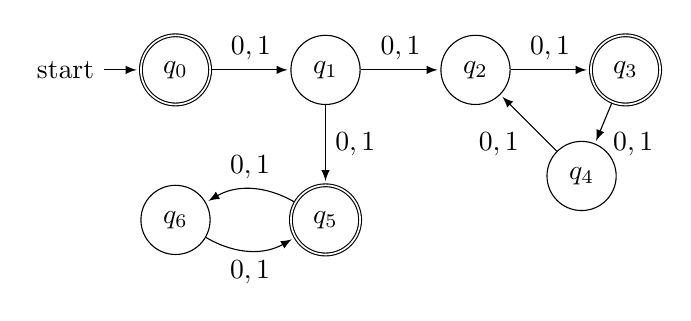
\begin{tikzpicture}[>=latex, shorten >=1pt,node distance=0.75in, on grid, auto]
		\node[state,initial,accepting] (q0) {$q_0$};
		\node[state](q1) [right=of q0] {$q_1$};
		\node[state](q2) [right=of q1] {$q_2$};
		\node[state,accepting](q3) [right=of q2] {$q_3$};
		\node[state] (q4) [below right=of q2] {$q_4$};
		\node[state,accepting](q5) [below=of q1] {$q_5$};
		\node[state] (q6) [left=of q5] {$q_6$};
		\path[->]
		(q0) edge node {$0,1$} (q1)
		(q1) edge node {$0,1$} (q2)
		(q2) edge node {$0,1$} (q3)
		(q3) edge node {$0,1$} (q4)
		(q4) edge node {$0,1$} (q2)
		(q1) edge node {$0,1$} (q5)
		(q5) edge [bend right,swap] node {$0,1$} (q6)	
		(q6) edge [bend right,swap] node {$0,1$} (q5);
		\end{tikzpicture} 
		\caption{$((0+1)(0+1))^\ast+((0+1)(0+1(0+1))^\ast$的等价$FA$}
		\label{fig:0101FA}
	\end{figure}
	\begin{figure}[htbp]
		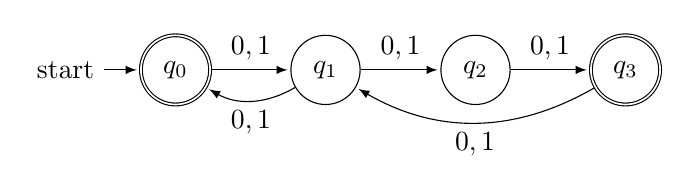
\begin{tikzpicture}[>=latex, shorten >=1pt,node distance=0.75in, on grid, auto]
		\node[state,initial,accepting] (q0) {$q_0$};
		\node[state](q1) [right=of q0] {$q_1$};
		\node[state](q2) [right=of q1] {$q_2$};
		\node[state,accepting](q3) [right=of q2] {$q_3$};
		\path[->]
		(q0) edge node {$0,1$} (q1)
		(q1) edge node {$0,1$} (q2)
		(q2) edge node {$0,1$} (q3)
		(q1) edge [bend left] node {$0,1$} (q0)	
		(q3) edge [bend left] node {$0,1$} (q1);
		\end{tikzpicture} 
		\caption{$((0+1)(0+1))^\ast+((0+1)(0+1(0+1))^\ast$的\emph{不等价}$FA$}
		\label{fig:0101-1FA}
	\end{figure}
	\begin{figure}[htbp]
		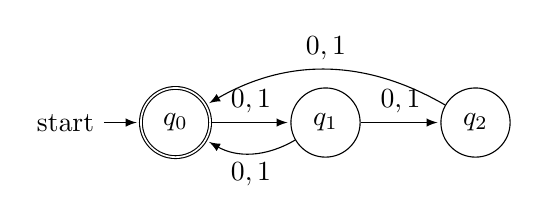
\begin{tikzpicture}[>=latex, shorten >=1pt,node distance=0.75in, on grid, auto]
		\node[state,initial,accepting] (q0) {$q_0$};
		\node[state](q1) [right=of q0] {$q_1$};
		\node[state](q2) [right=of q1] {$q_2$};
		\path[->]
		(q0) edge node {$0,1$} (q1)
		(q1) edge node {$0,1$} (q2)
		(q2) edge [bend right,swap] node {$0,1$} (q0)	
		(q1) edge [bend left] node {$0,1$} (q0);
		\end{tikzpicture} 
		\caption{$((0+1)(0+1))^\ast+((0+1)(0+1(0+1))^\ast$的\emph{不等价}$FA$}
		\label{fig:0101-2FA}
	\end{figure}
	\begin{figure}[htbp]
		\centering
		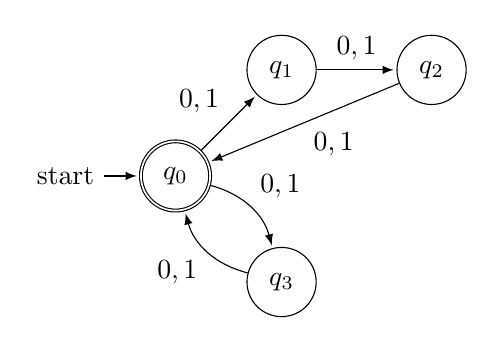
\begin{tikzpicture}[>=latex, shorten >=1pt,node distance=0.75in, on grid, auto]
		\node[state,initial,accepting] (q0) {$q_0$};
		\node[state](q1) [above right=of q0] {$q_1$};
		\node[state](q2) [right=of q1] {$q_2$};
		\node[state](q3) [below right=of q0] {$q_3$};
		\path[->]
		(q0) edge node {$0,1$} (q1)
		(q1) edge node {$0,1$} (q2)
		(q2) edge node {$0,1$} (q0)
		(q0) edge [bend left] node {$0,1$} (q3)	
		(q3) edge [bend left] node {$0,1$} (q0);
		\end{tikzpicture} 
		\caption{$((0+1)(0+1))^\ast+((0+1)(0+1(0+1))^\ast$的\emph{不等价}$FA$}
		\label{fig:0101-3FA}
	\end{figure}

\end{solution}
	

%%%%%%%%%%%%%%%%%%%%%%%%%%%%%%%%%%%%%%%%%%%%%%%%

\section{正则代换(regular substitution)}

设$\Sigma,\Delta$是两个字母表,映射
$$f:\Sigma \to 2^{\Delta^{\ast}}$$
被称为是从$\Sigma$到$\Delta$的
\textbf{代换}。如果对于$\forall a\in \Sigma,f(a)$是$\Delta$上的$RL$,则称\textbf{$f$为正则代换}。

\begin{itemize}
	\item 现将$f$的定义域扩展到$\Sigma^{\ast}$上:
	\begin{enumerate}
		\item $f(\epsilon) =\{\epsilon\}$
		\item $f(xa)=f(x)f(a)$
	\end{enumerate}
	\item 再将$f$的定义域扩展到$2^{\Delta^{\ast}}$\\
	对于$\forall L\subseteq \Sigma{\ast}$\\
	$f(L) = \bigcup\limits_{x\in L} f(x)$
	\item $f$是正则代换,则
	\begin{enumerate}
		\item $f(\emptyset)=\emptyset$
		\item $f(\epsilon)=\epsilon$
		\item 对于$\forall a\in \Sigma,f(a)$是$\Delta$上的$RE$
		\item 如果$r,s$是$\Sigma$上的$RE$,则\\
		$f(r+s)=f(r)+f(s)$\\
		$f(rs)=f(r)f(s)$\\
		$f(r^{\ast}={f(r)}^{\ast}$\\
		是$\Delta$上的$RE$
	\end{enumerate}
\end{itemize}

\begin{example}
	设$\Sigma={0,1},\Delta={a,b},f(0)=a,f(1)=b^{\ast}$, 则
	\begin{align*}
	f(010) &= f(0)f(1)f(0)=ab^{\ast}a\\
	f({11,00})&=f(11)\cup f(00) \\
	&=f(1)f(1)\cup f(0)f(0)\\
	&=b^{\ast}b^{\ast}+aa = b^{\ast}+aa \\
	f(L(0^{\ast}(0+1)1^{\ast})) &= L(a^{\ast}(a+b^{\ast}){(b^{\ast})}^{\ast})\\
	&= L(a^{\ast}(a+b^{\ast})b^{\ast})\\
	&= L(a^{\ast}ab^{\ast} + a^{\ast}b^{\ast}b^{\ast})\\
	&= L(a^{\ast}b^{\ast})
	\end{align*}
\end{example}

\begin{theorem}
	设$L$是$\Sigma$上的一个$RL$
	$$f:\Sigma \to 2^{\Delta^{\ast}}$$
	是正则代换,则$f(L)$也是$RL$. \hfill$\square$ 
\end{theorem}
\begin{proof}
	描述工具$RE$
	
	对$r$中运算符的个数$n$施以归纳,证明$f(r)$是表示$f(L)$的$RE$.
	\begin{itemize}
		\item 当$n=0$时, 结论成立。
		\item 当$n\le k$时,定理成立,即当$r$中运算符的个数不大于$k$时:$f(L(r)) = L(f(r))$。
		\item 当$n=k+1$时,
		\begin{enumerate}
			\item $r=r_1 + r_2$
			\begin{align*}
			f(L) &= f(L(r)) \\
			&=f(L(r_1 + r_2))\\
			&=f(L(r_1)\cup L(r_2))  &\qquad  \text{$RE$的定义} \\
			&=f(L(r_1))\cup f(L(r_2)) &\qquad \text{正则代换的定义} \\
			&=L(f(r_1))\cup L(f(r_2)) &\qquad \text{归纳假设} \\
			&=L(f(r_1)+f(r_2)) &\qquad RE\text{的定义} \\
			&=L(f(r_1+r_2)) &\qquad RE\text{的正则代换的定义} \\
			&=L(f(r))
			\end{align*}
			
			\item $r=r_1r_2$
			\begin{align*}
			f(L) &=f(L(r)) \\
			&=f(L(r_1r_2))\\
			&=f(L(r_1)L(r2)) &\qquad \text{$RE$的定义}\\
			&=f(L(r_1))f(L(r_2)) &\qquad \text{正则代换的定义}\\
			&=L(f(r_1))L(f(r_2)) &\qquad \text{归纳假设} \\
			&=L(f(r_1)f(r_2)) &\qquad \text{$RE$的定义}\\
			&=L(f(r_1r_2)) &\qquad \text{$RE$的正则代换的定义}\\
			&=L(f(r_1r_2))
			\end{align*}
			
			\item $r={r_1}^{\ast}$
			\begin{align*}
			f(L) &=f(L(r)) \\
			&=f(L({r_1}^{\ast}))\\
			&=f(L({r_1})^{\ast}) &\qquad \text{$RE$的定义}\\
			&={(f(L({r_1})))}^{\ast} &\qquad \text{正则代换的定义}\\
			&={(L(f(r_1)))}^{\ast} &\qquad \text{归纳假设} \\
			&=L(f(r_1)^{\ast}) &\qquad \text{$RE$的定义}\\
			&=L(f({r_1}^{\ast})) &\qquad \text{$RE$的正则代换的定义}\\
			&=L(f(r))
			\end{align*}
		\end{enumerate}
	\end{itemize}  \hfill$\square$ 
\end{proof}
 % \cite{蒋宗礼2013}(第4章 正则表达式)
%%%%%%%%%%%%%%%%%%%%%% chapter.tex %%%%%%%%%%%%%%%%%%%%%%%%%%%%%%%%%
%
% sample chapter
%
% Use this file as a template for your own input.
%
%%%%%%%%%%%%%%%%%%%%%%%% Springer-Verlag %%%%%%%%%%%%%%%%%%%%%%%%%%
%\motto{Use the template \emph{chapter.tex} to style the various elements of your chapter content.}
\chapter{chapter format}
\label{intro} % Always give a unique label
% use \chaptermark{}
% to alter or adjust the chapter heading in the running head

\abstract{This paragraph shall summarize the contents of the paper in short terms.}

\paragraph{first Paragraph}
\subparagraph{first Subparagraph} 
\section{first section}
\label{first_section} % Always give a unique label
\subsection{first subsection}

\begin{svgraybox}
	emphasize complete paragraphs of texts 
\end{svgraybox}

description
\begin{description}[Type 1]
	\item[Type 1]{description type 1.}
	\item[Type 2]{description type 2.}
\end{description}

Problems or Exercises should be sorted chapterwise
\section*{Problems}
\addcontentsline{toc}{section}{Problems}
%
% Use the following environment.
% Don't forget to label each problem;
% the label is needed for the solutions' environment
\begin{prob}
	\label{prob1}
	A given problem or Excercise is described here. 
\end{prob}

\begin{prob}
	\label{prob2}
	\textbf{Problem Heading}\\
	(a) The first part of the problem is described here.\\
	(b) The second part of the problem is described here.
\end{prob}


\section{theorem/definition/proof/example}
\begin{theorem}
	Theorem text goes here.
\end{theorem}

%
\begin{definition}[DfName]
	Definition text goes here.
\end{definition}

\begin{proof}
	%\smartqed
	Proof text goes here.
	\qed
\end{proof}

\begin{example}
	Examples text goes here.  \hfill$\square$ 
\end{example}

\begin{corollary}
	Examples text goes here.  \hfill$\square$ 
\end{corollary}

\begin{lemma}
	Examples text goes here.  \hfill$\square$ 
\end{lemma}

\begin{remark}
	Examples text goes here.  \hfill$\square$ 
\end{remark}

\begin{proposition}
	Examples text goes here.  \hfill$\square$ 
\end{proposition}

\begin{property}
	Examples text goes here.  \hfill$\square$ 
\end{property}

\begin{note}
	Examples text goes here.
\end{note}

\begin{problem}
	Examples text goes here.
\end{problem}

\begin{question}
	Examples text goes here.
\end{question}

\begin{exercise}
	Examples text goes here.  
\end{exercise}

\begin{solution}
	Examples text goes here.  
\end{solution}


\section{equation}
equations, e.g.
\begin{equation}
a \times b = c\;,
\end{equation}

multiline equations
\begin{eqnarray}
a \times b = c \nonumber\\
\vec{a} \cdot \vec{b}=\vec{c}
\label{eq:01}
\end{eqnarray}

enumerate example
\begin{enumerate}
	\item{item 1.}
	\begin{enumerate}
		\item{sub item a.}
		\item{sub item b.}
	\end{enumerate}
	\item{item 2.}
\end{enumerate}

itemize example
\begin{itemize}
	\item{item 1, cf. Table~\ref{tab:1}.}
	\begin{itemize}
		\item{sub item 1.}
		\item{sub item 2.}
	\end{itemize}
	\item{item.}
\end{itemize}

For tables use
\begin{table}
	\caption{Please write your table caption here}
	\label{tab:1}       % Give a unique label
	%
	% For LaTeX tables use
	%
	\begin{tabular}{p{2cm}p{2.4cm}p{2cm}p{4.9cm}}
		\hline\noalign{\smallskip}
		Classes & Subclass & Length & Action Mechanism  \\
		\noalign{\smallskip}\svhline\noalign{\smallskip}
		Translation & mRNA$^a$  & 22 (19--25) & Translation repression, mRNA cleavage\\
		Translation & mRNA cleavage & 21 & mRNA cleavage\\
		Translation & mRNA  & 21--22 & mRNA cleavage\\
		Translation & mRNA  & 24--26 & Histone and DNA Modification\\
		\noalign{\smallskip}\hline\noalign{\smallskip}
	\end{tabular}
	$^a$ Table foot note (with superscript)
\end{table}

\section{figure}

For figures use
\begin{figure}[htbp]
\sidecaption
% Use the relevant command for your figure-insertion program
% to insert the figure file.
% For example, with the option graphics use
\includegraphics[scale=.65]{figure}
%
% If not, use
%\picplace{5cm}{2cm} % Give the correct figure height and width in cm
%
\caption{If the width of the figure is less than 7.8 cm use the \texttt{sidecapion} command to flush the caption on the left side of the page. If the figure is positioned at the top of the page, align the sidecaption with the top of the figure -- to achieve this you simply need to use the optional argument \texttt{[t]} with the \texttt{sidecaption} command}
\label{fig:1}       % Give a unique label
\end{figure}


\begin{figure}[htbp]
\sidecaption[t]
% Use the relevant command for your figure-insertion program
% to insert the figure file.
% For example, with the option graphics use
\includegraphics[scale=.65]{figure}
%
% If not, use
%\picplace{5cm}{2cm} % Give the correct figure height and width in cm
%
\caption{Please write your figure caption here}
\label{fig:2}       % Give a unique label
\end{figure}


\section{ref,cite}
\label{sec:2}
% Always give a unique label
% and use \ref{<label>} for cross-references
% and \cite{<label>} for bibliographic references
% use \sectionmark{}
% to alter or adjust the section heading in the running head

referenc Sect.~\ref{sec:2} , see also Fig.~\ref{fig:1}

referenc:Table. ~\ref{tab:1}

\cite{Lipschutz2007}

\cite[chap.2]{Lipschutz2007}


\runinhead{Run-in Heading Boldface Version} Use the \LaTeX\ automatism for all your cross-references and citations.
\subruninhead{Run-in Heading Italic Version} Use the \LaTeX\ automatism for all your cross-refer\-ences and citations as has already been described in Sect.~\ref{sec:2}\index{paragraph}.
% Use the \index{} command to code your index words
%

\begin{quotation}
	引用原文-- it will automatically render Springer's preferred layout.
\end{quotation}

footnote environment \footnote{脚注footnote.}.

\begin{algorithm}  
	\caption{用归并排序求逆序数}  \label{key}
	\begin{algorithmic}[1] %每行显示行号  
		\Require $M=(Q,V,T,_,F)$  
		\Ensure The equivalence classes of $Q$  
		\Function {MergerSort}{$Array, left, right$}  
		\State $result \gets 0$  
		\If {$left < right$}  
		\State $middle \gets (left + right) / 2$  
		\State $result \gets result +$ \Call{MergerSort}{$Array, left, middle$}  
		\State $result \gets result +$ \Call{MergerSort}{$Array, middle, right$}  
		\State $result \gets result +$ \Call{Merger}{$Array,left,middle,right$}  
		\EndIf  
		\State \Return{$result$}  
		\EndFunction 
	\end{algorithmic}   
\end{algorithm}

\begin{algorithm}[!htbp]
	\SetKwInOut{KIN}{在这里自定义输入名称}
	\SetKwInOut{KOUT}{在这里自定义输出名称}
	\caption{在这里编写算法名}
	\label{key}
	\KIN{在这里编写输入参数1,参数2...}% 输入参数
	\KOUT{在这里编写输出参数1,参数2...}% 输出
	算法第一行\\
	%循环语句%
	\For{$i \leftarrow 1$ to $N$} {
		\If{$a > b$} {
			if语句。
		}
		\ElseIf{$b > c$} {
			elseif语句。
		}
		\Else {
			else语句。
		}
	}
\end{algorithm}

%%%%%%%%%%%%%%%%%%%%%%%%%%%%%%%
\begin{comment}

\Function {"FuncName"}{}
%if
\If {"condition"}  "text"   \EndIf
\State

% if else
\If  {"condition"}   "text"   
\Else   "text"    
\EndIf\State                

%if  elseif else
\If  {"condition"}     "text"   
\ElsIf {"condition"}   "text"       
\Else   "text"  
\EndIf\State

%for
\For{"condition"}   "text"   \EndFor\State

%forall
\ForAll {"condition"}  "text"  \EndFor\State

%while
\While {"condition"}  "text"  \EndWhile\State

%repeat
\Repeat "text"  \Until {"condition"}\State

%loop
\Loop "text"  \EndLoop\State
%return
\Return $Result$
\EndFunction

\end{comment}

%%%%%%%%%%%%%%%%%%%%%%%%%%%%%%%%%%%%%%%%%%%%%%%%%5555
%\usepackage{tabulary}
%tabulary tries to balance the column widths so that each column has at least its natural width, without exceeding the maximum length. 

\begin{center}
	\begin{tabulary}{0.7\textwidth}{|L|C|L|}
		Short sentences      & \#  & Long sentences                                                 \\
		\hline
		This is short.       & 173 & This is much loooooooonger, because there are many more words.  \\
		This is not shorter. & 317 & This is still loooooooonger, because there are many more words. \\
	\end{tabulary}  
\end{center}

\begin{comment}
L  left-justified balanced column 
C  centered balanced column 
R  right-justified balanced column 
J  left-right-justified balanced column 
\end{comment}

参考文献
%%%%%%%%%%%%%%%%%%%%%%%%% referenc.tex %%%%%%%%%%%%%%%%%%%%%%%%%%%%%%
% sample references
% %
% Use this file as a template for your own input.
%
%%%%%%%%%%%%%%%%%%%%%%%% Springer-Verlag %%%%%%%%%%%%%%%%%%%%%%%%%%
%
% BibTeX users please use
% \bibliographystyle{}
% \bibliography{}
%
\biblstarthook{In view of the parallel print and (chapter-wise) online publication of your book at \url{www.springerlink.com} it has been decided that -- as a genreral rule --  references should be sorted chapter-wise and placed at the end of the individual chapters. However, upon agreement with your contact at Springer you may list your references in a single seperate chapter at the end of your book. Deactivate the class option \texttt{sectrefs} and the \texttt{thebibliography} environment will be put out as a chapter of its own.\\\indent
References may be \textit{cited} in the text either by number (preferred) or by author/year.\footnote{Make sure that all references from the list are cited in the text. Those not cited should be moved to a separate \textit{Further Reading} section or chapter.} The reference list should ideally be \textit{sorted} in alphabetical order -- even if reference numbers are used for the their citation in the text. If there are several works by the same author, the following order should be used: 
\begin{enumerate}
\item all works by the author alone, ordered chronologically by year of publication
\item all works by the author with a coauthor, ordered alphabetically by coauthor
\item all works by the author with several coauthors, ordered chronologically by year of publication.
\end{enumerate}
The \textit{styling} of references\footnote{Always use the standard abbreviation of a journal's name according to the ISSN \textit{List of Title Word Abbreviations}, see \url{http://www.issn.org/en/node/344}} depends on the subject of your book:
\begin{itemize}
\item The \textit{two} recommended styles for references in books on \textit{mathematical, physical, statistical and computer sciences} are depicted in ~\cite{science-contrib, science-online, science-mono, science-journal, science-DOI} and ~\cite{phys-online, phys-mono, phys-journal, phys-DOI, phys-contrib}.
\item Examples of the most commonly used reference style in books on \textit{Psychology, Social Sciences} are~\cite{psysoc-mono, psysoc-online,psysoc-journal, psysoc-contrib, psysoc-DOI}.
\item Examples for references in books on \textit{Humanities, Linguistics, Philosophy} are~\cite{humlinphil-journal, humlinphil-contrib, humlinphil-mono, humlinphil-online, humlinphil-DOI}.
\item Examples of the basic Springer style used in publications on a wide range of subjects such as \textit{Computer Science, Economics, Engineering, Geosciences, Life Sciences, Medicine, Biomedicine} are ~\cite{basic-contrib, basic-online, basic-journal, basic-DOI, basic-mono}. 
\end{itemize}
}

\begin{thebibliography}{99.}%
% and use \bibitem to create references.
%
% Use the following syntax and markup for your references if 
% the subject of your book is from the field 
% "Mathematics, Physics, Statistics, Computer Science"
%
% Contribution 
\bibitem{science-contrib} Broy, M.: Software engineering --- from auxiliary to key technologies. In: Broy, M., Dener, E. (eds.) Software Pioneers, pp. 10-13. Springer, Heidelberg (2002)
%
% Online Document
\bibitem{science-online} Dod, J.: Effective substances. In: The Dictionary of Substances and Their Effects. Royal Society of Chemistry (1999) Available via DIALOG. \\
\url{http://www.rsc.org/dose/title of subordinate document. Cited 15 Jan 1999}
%
% Monograph
\bibitem{science-mono} Geddes, K.O., Czapor, S.R., Labahn, G.: Algorithms for Computer Algebra. Kluwer, Boston (1992) 
%
% Journal article
\bibitem{science-journal} Hamburger, C.: Quasimonotonicity, regularity and duality for nonlinear systems of partial differential equations. Ann. Mat. Pura. Appl. \textbf{169}, 321--354 (1995)
%
% Journal article by DOI
\bibitem{science-DOI} Slifka, M.K., Whitton, J.L.: Clinical implications of dysregulated cytokine production. J. Mol. Med. (2000) doi: 10.1007/s001090000086 
%
\bigskip

% Use the following (APS) syntax and markup for your references if 
% the subject of your book is from the field 
% "Mathematics, Physics, Statistics, Computer Science"
%
% Online Document
\bibitem{phys-online} J. Dod, in \textit{The Dictionary of Substances and Their Effects}, Royal Society of Chemistry. (Available via DIALOG, 1999), 
\url{http://www.rsc.org/dose/title of subordinate document. Cited 15 Jan 1999}
%
% Monograph
\bibitem{phys-mono} H. Ibach, H. L\"uth, \textit{Solid-State Physics}, 2nd edn. (Springer, New York, 1996), pp. 45-56 
%
% Journal article
\bibitem{phys-journal} S. Preuss, A. Demchuk Jr., M. Stuke, Appl. Phys. A \textbf{61}
%
% Journal article by DOI
\bibitem{phys-DOI} M.K. Slifka, J.L. Whitton, J. Mol. Med., doi: 10.1007/s001090000086
%
% Contribution 
\bibitem{phys-contrib} S.E. Smith, in \textit{Neuromuscular Junction}, ed. by E. Zaimis. Handbook of Experimental Pharmacology, vol 42 (Springer, Heidelberg, 1976), p. 593
%
\bigskip
%
% Use the following syntax and markup for your references if 
% the subject of your book is from the field 
% "Psychology, Social Sciences"
%
%
% Monograph
\bibitem{psysoc-mono} Calfee, R.~C., \& Valencia, R.~R. (1991). \textit{APA guide to preparing manuscripts for journal publication.} Washington, DC: American Psychological Association.
%
% Online Document
\bibitem{psysoc-online} Dod, J. (1999). Effective substances. In: The dictionary of substances and their effects. Royal Society of Chemistry. Available via DIALOG. \\
\url{http://www.rsc.org/dose/Effective substances.} Cited 15 Jan 1999.
%
% Journal article
\bibitem{psysoc-journal} Harris, M., Karper, E., Stacks, G., Hoffman, D., DeNiro, R., Cruz, P., et al. (2001). Writing labs and the Hollywood connection. \textit{J Film} Writing, 44(3), 213--245.
%
% Contribution 
\bibitem{psysoc-contrib} O'Neil, J.~M., \& Egan, J. (1992). Men's and women's gender role journeys: Metaphor for healing, transition, and transformation. In B.~R. Wainrig (Ed.), \textit{Gender issues across the life cycle} (pp. 107--123). New York: Springer.
%
% Journal article by DOI
\bibitem{psysoc-DOI}Kreger, M., Brindis, C.D., Manuel, D.M., Sassoubre, L. (2007). Lessons learned in systems change initiatives: benchmarks and indicators. \textit{American Journal of Community Psychology}, doi: 10.1007/s10464-007-9108-14.
%
%
% Use the following syntax and markup for your references if 
% the subject of your book is from the field 
% "Humanities, Linguistics, Philosophy"
%
\bigskip
%
% Journal article
\bibitem{humlinphil-journal} Alber John, Daniel C. O'Connell, and Sabine Kowal. 2002. Personal perspective in TV interviews. \textit{Pragmatics} 12:257--271
%
% Contribution 
\bibitem{humlinphil-contrib} Cameron, Deborah. 1997. Theoretical debates in feminist linguistics: Questions of sex and gender. In \textit{Gender and discourse}, ed. Ruth Wodak, 99--119. London: Sage Publications.
%
% Monograph
\bibitem{humlinphil-mono} Cameron, Deborah. 1985. \textit{Feminism and linguistic theory.} New York: St. Martin's Press.
%
% Online Document
\bibitem{humlinphil-online} Dod, Jake. 1999. Effective substances. In: The dictionary of substances and their effects. Royal Society of Chemistry. Available via DIALOG. \\
http://www.rsc.org/dose/title of subordinate document. Cited 15 Jan 1999
%
% Journal article by DOI
\bibitem{humlinphil-DOI} Suleiman, Camelia, Daniel C. O�Connell, and Sabine Kowal. 2002. `If you and I, if we, in this later day, lose that sacred fire...�': Perspective in political interviews. \textit{Journal of Psycholinguistic Research}. doi: 10.1023/A:1015592129296.
%
%
%
\bigskip
%
%
% Use the following syntax and markup for your references if 
% the subject of your book is from the field 
% "Computer Science, Economics, Engineering, Geosciences, Life Sciences"
%
%
% Contribution 
\bibitem{basic-contrib} Brown B, Aaron M (2001) The politics of nature. In: Smith J (ed) The rise of modern genomics, 3rd edn. Wiley, New York 
%
% Online Document
\bibitem{basic-online} Dod J (1999) Effective Substances. In: The dictionary of substances and their effects. Royal Society of Chemistry. Available via DIALOG. \\
\url{http://www.rsc.org/dose/title of subordinate document. Cited 15 Jan 1999}
%
% Journal article by DOI
\bibitem{basic-DOI} Slifka MK, Whitton JL (2000) Clinical implications of dysregulated cytokine production. J Mol Med, doi: 10.1007/s001090000086
%
% Journal article
\bibitem{basic-journal} Smith J, Jones M Jr, Houghton L et al (1999) Future of health insurance. N Engl J Med 965:325--329
%
% Monograph
\bibitem{basic-mono} South J, Blass B (2001) The future of modern genomics. Blackwell, London 
%
\end{thebibliography}


\begin{thebibliography}{99}
	
	
	\bibitem{Lipschutz2007}
	S. Lipschutz and M. L. Lipson, \textit{Schaum's Outline of Theory and Problems of Discrete Mathematics}, Third Edition, New York: McGraw-Hill, 2007.
	
	\bibitem{Rosen2007}
	K. H. Rosen, \textit{Discrete Mathematics and Its Applications}, Seventh Edition, New York: McGraw-Hill, 2007.
	
	\bibitem{Maclane1988}
	S. Maclane and G. Birkhoff, \textit{Algebra}, Third Edition, New York: Bchelsea Publishing Company, 1988.
\end{thebibliography}
     % 整理的简单格式样例 
%%%%%%%%%%%%%%%%%%%%%% chapter.tex %%%%%%%%%%%%%%%%%%%%%%%%%%%%%%%%%
%
% sample chapter
%
% Use this file as a template for your own input.
%
%%%%%%%%%%%%%%%%%%%%%%%% Springer-Verlag %%%%%%%%%%%%%%%%%%%%%%%%%%
%\motto{Use the template \emph{chapter.tex} to style the various elements of your chapter content.}
\chapter{Chapter Heading}
\label{intro} % Always give a unique label
% use \chaptermark{}
% to alter or adjust the chapter heading in the running head

\abstract*{Each chapter should be preceded by an abstract (10--15 lines long) that summarizes the content. The abstract will appear \textit{online} at \url{www.SpringerLink.com} and be available with unrestricted access. This allows unregistered users to read the abstract as a teaser for the complete chapter. As a general rule the abstracts will not appear in the printed version of your book unless it is the style of your particular book or that of the series to which your book belongs.
Please use the 'starred' version of the new Springer \texttt{abstract} command for typesetting the text of the online abstracts (cf. source file of this chapter template \texttt{abstract}) and include them with the source files of your manuscript. Use the plain \texttt{abstract} command if the abstract is also to appear in the printed version of the book.}

\abstract{Each chapter should be preceded by an abstract (10--15 lines long) that summarizes the content. The abstract will appear \textit{online} at \url{www.SpringerLink.com} and be available with unrestricted access. This allows unregistered users to read the abstract as a teaser for the complete chapter. As a general rule the abstracts will not appear in the printed version of your book unless it is the style of your particular book or that of the series to which your book belongs.\newline\indent
Please use the 'starred' version of the new Springer \texttt{abstract} command for typesetting the text of the online abstracts (cf. source file of this chapter template \texttt{abstract}) and include them with the source files of your manuscript. Use the plain \texttt{abstract} command if the abstract is also to appear in the printed version of the book.}

\section{Section Heading}
\label{sec:1}
Use the template \emph{chapter.tex} together with the Springer document class SVMono (monograph-type books) or SVMult (edited books) to style the various elements of your chapter content in the Springer layout.

\section{Section Heading}
\label{sec:2}
% Always give a unique label
% and use \ref{<label>} for cross-references
% and \cite{<label>} for bibliographic references
% use \sectionmark{}
% to alter or adjust the section heading in the running head
Instead of simply listing headings of different levels we recommend to let every heading be followed by at least a short passage of text. Furtheron please use the \LaTeX\ automatism for all your cross-references and citations.

Please note that the first line of text that follows a heading is not indented, whereas the first lines of all subsequent paragraphs are.

Use the standard \verb|equation| environment to typeset your equations, e.g.
%
\begin{equation}
a \times b = c\;,
\end{equation}
%
however, for multiline equations we recommend to use the \verb|eqnarray|
environment\footnote{In physics texts please activate the class option \texttt{vecphys} to depict your vectors in \textbf{\itshape boldface-italic} type - as is customary for a wide range of physical subjects.}.
\begin{eqnarray}
a \times b = c \nonumber\\
\vec{a} \cdot \vec{b}=\vec{c}
\label{eq:01}
\end{eqnarray}

\subsection{Subsection Heading}
\label{subsec:2}
Instead of simply listing headings of different levels we recommend to let every heading be followed by at least a short passage of text. Furtheron please use the \LaTeX\ automatism for all your cross-references\index{cross-references} and citations\index{citations} as has already been described in Sect.~\ref{sec:2}.

\begin{quotation}
Please do not use quotation marks when quoting texts! Simply use the \verb|quotation| environment -- it will automatically render Springer's preferred layout.
\end{quotation}


\subsubsection{Subsubsection Heading}
Instead of simply listing headings of different levels we recommend to let every heading be followed by at least a short passage of text. Furtheron please use the \LaTeX\ automatism for all your cross-references and citations as has already been described in Sect.~\ref{subsec:2}, see also Fig.~\ref{fig:1}\footnote{If you copy text passages, figures, or tables from other works, you must obtain \textit{permission} from the copyright holder (usually the original publisher). Please enclose the signed permission with the manucript. The sources\index{permission to print} must be acknowledged either in the captions, as footnotes or in a separate section of the book.}

Please note that the first line of text that follows a heading is not indented, whereas the first lines of all subsequent paragraphs are.

% For figures use
%
\begin{figure}[b]
\sidecaption
% Use the relevant command for your figure-insertion program
% to insert the figure file.
% For example, with the option graphics use
\includegraphics[scale=.65]{figure}
%
% If not, use
%\picplace{5cm}{2cm} % Give the correct figure height and width in cm
%
\caption{If the width of the figure is less than 7.8 cm use the \texttt{sidecapion} command to flush the caption on the left side of the page. If the figure is positioned at the top of the page, align the sidecaption with the top of the figure -- to achieve this you simply need to use the optional argument \texttt{[t]} with the \texttt{sidecaption} command}
\label{fig:1}       % Give a unique label
\end{figure}


\paragraph{Paragraph Heading} %
Instead of simply listing headings of different levels we recommend to let every heading be followed by at least a short passage of text. Furtheron please use the \LaTeX\ automatism for all your cross-references and citations as has already been described in Sect.~\ref{sec:2}.

Please note that the first line of text that follows a heading is not indented, whereas the first lines of all subsequent paragraphs are.

For typesetting numbered lists we recommend to use the \verb|enumerate| environment -- it will automatically render Springer's preferred layout.

\begin{enumerate}
\item{Livelihood and survival mobility are oftentimes coutcomes of uneven socioeconomic development.}
\begin{enumerate}
\item{Livelihood and survival mobility are oftentimes coutcomes of uneven socioeconomic development.}
\item{Livelihood and survival mobility are oftentimes coutcomes of uneven socioeconomic development.}
\end{enumerate}
\item{Livelihood and survival mobility are oftentimes coutcomes of uneven socioeconomic development.}
\end{enumerate}


\subparagraph{Subparagraph Heading} In order to avoid simply listing headings of different levels we recommend to let every heading be followed by at least a short passage of text. Use the \LaTeX\ automatism for all your cross-references and citations as has already been described in Sect.~\ref{sec:2}, see also Fig.~\ref{fig:2}.

Please note that the first line of text that follows a heading is not indented, whereas the first lines of all subsequent paragraphs are.

For unnumbered list we recommend to use the \verb|itemize| environment -- it will automatically render Springer's preferred layout.

\begin{itemize}
\item{Livelihood and survival mobility are oftentimes coutcomes of uneven socioeconomic development, cf. Table~\ref{tab:1}.}
\begin{itemize}
\item{Livelihood and survival mobility are oftentimes coutcomes of uneven socioeconomic development.}
\item{Livelihood and survival mobility are oftentimes coutcomes of uneven socioeconomic development.}
\end{itemize}
\item{Livelihood and survival mobility are oftentimes coutcomes of uneven socioeconomic development.}
\end{itemize}

\begin{figure}[t]
\sidecaption[t]
% Use the relevant command for your figure-insertion program
% to insert the figure file.
% For example, with the option graphics use
\includegraphics[scale=.65]{figure}
%
% If not, use
%\picplace{5cm}{2cm} % Give the correct figure height and width in cm
%
\caption{Please write your figure caption here}
\label{fig:2}       % Give a unique label
\end{figure}

\runinhead{Run-in Heading Boldface Version} Use the \LaTeX\ automatism for all your cross-references and citations as has already been described in Sect.~\ref{sec:2}.

\subruninhead{Run-in Heading Italic Version} Use the \LaTeX\ automatism for all your cross-refer\-ences and citations as has already been described in Sect.~\ref{sec:2}\index{paragraph}.
% Use the \index{} command to code your index words
%
% For tables use
%
\begin{table}
\caption{Please write your table caption here}
\label{tab:1}       % Give a unique label
%
% For LaTeX tables use
%
\begin{tabular}{p{2cm}p{2.4cm}p{2cm}p{4.9cm}}
\hline\noalign{\smallskip}
Classes & Subclass & Length & Action Mechanism  \\
\noalign{\smallskip}\svhline\noalign{\smallskip}
Translation & mRNA$^a$  & 22 (19--25) & Translation repression, mRNA cleavage\\
Translation & mRNA cleavage & 21 & mRNA cleavage\\
Translation & mRNA  & 21--22 & mRNA cleavage\\
Translation & mRNA  & 24--26 & Histone and DNA Modification\\
\noalign{\smallskip}\hline\noalign{\smallskip}
\end{tabular}
$^a$ Table foot note (with superscript)
\end{table}
%
\section{Section Heading}
\label{sec:3}
% Always give a unique label
% and use \ref{<label>} for cross-references
% and \cite{<label>} for bibliographic references
% use \sectionmark{}
% to alter or adjust the section heading in the running head
Instead of simply listing headings of different levels we recommend to let every heading be followed by at least a short passage of text. Furtheron please use the \LaTeX\ automatism for all your cross-references and citations as has already been described in Sect.~\ref{sec:2}.

Please note that the first line of text that follows a heading is not indented, whereas the first lines of all subsequent paragraphs are.

If you want to list definitions or the like we recommend to use the Springer-enhanced \verb|description| environment -- it will automatically render Springer's preferred layout.

\begin{description}[Type 1]
\item[Type 1]{That addresses central themes pertainng to migration, health, and disease. In Sect.~\ref{sec:1}, Wilson discusses the role of human migration in infectious disease distributions and patterns.}
\item[Type 2]{That addresses central themes pertainng to migration, health, and disease. In Sect.~\ref{subsec:2}, Wilson discusses the role of human migration in infectious disease distributions and patterns.}
\end{description}

\subsection{Subsection Heading} %
In order to avoid simply listing headings of different levels we recommend to let every heading be followed by at least a short passage of text. Use the \LaTeX\ automatism for all your cross-references and citations citations as has already been described in Sect.~\ref{sec:2}.

Please note that the first line of text that follows a heading is not indented, whereas the first lines of all subsequent paragraphs are.

\begin{svgraybox}
If you want to emphasize complete paragraphs of texts we recommend to use the newly defined Springer class option \verb|graybox| and the newly defined environment \verb|svgraybox|. This will produce a 15 percent screened box 'behind' your text.

If you want to emphasize complete paragraphs of texts we recommend to use the newly defined Springer class option and environment \verb|svgraybox|. This will produce a 15 percent screened box 'behind' your text.
\end{svgraybox}


\subsubsection{Subsubsection Heading}
Instead of simply listing headings of different levels we recommend to let every heading be followed by at least a short passage of text. Furtheron please use the \LaTeX\ automatism for all your cross-references and citations as has already been described in Sect.~\ref{sec:2}.

Please note that the first line of text that follows a heading is not indented, whereas the first lines of all subsequent paragraphs are.

\begin{theorem}
Theorem text goes here.
\end{theorem}
%
% or
%
\begin{definition}
Definition text goes here.
\end{definition}

\begin{proof}
%\smartqed
Proof text goes here.
\qed
\end{proof}

\paragraph{Paragraph Heading} %
Instead of simply listing headings of different levels we recommend to let every heading be followed by at least a short passage of text. Furtheron please use the \LaTeX\ automatism for all your cross-references and citations as has already been described in Sect.~\ref{sec:2}.

Note that the first line of text that follows a heading is not indented, whereas the first lines of all subsequent paragraphs are.
%
% For built-in environments use
%
\begin{theorem}
Theorem text goes here.
\end{theorem}
%
\begin{definition}
Definition text goes here.
\end{definition}
%
\begin{proof}
\smartqed
Proof text goes here.
\qed
\end{proof}
%
\begin{acknowledgement}
If you want to include acknowledgments of assistance and the like at the end of an individual chapter please use the \verb|acknowledgement| environment -- it will automatically render Springer's preferred layout.
\end{acknowledgement}
%
\section*{Appendix}
\addcontentsline{toc}{section}{Appendix}
%
When placed at the end of a chapter or contribution (as opposed to at the end of the book), the numbering of tables, figures, and equations in the appendix section continues on from that in the main text. Hence please \textit{do not} use the \verb|appendix| command when writing an appendix at the end of your chapter or contribution. If there is only one the appendix is designated ``Appendix'', or ``Appendix 1'', or ``Appendix 2'', etc. if there is more than one.

\begin{equation}
a \times b = c
\end{equation}
% Problems or Exercises should be sorted chapterwise
\section*{Problems}
\addcontentsline{toc}{section}{Problems}
%
% Use the following environment.
% Don't forget to label each problem;
% the label is needed for the solutions' environment
\begin{prob}
\label{prob1}
A given problem or Excercise is described here. The
problem is described here. The problem is described here.
\end{prob}

\begin{prob}
\label{prob2}
\textbf{Problem Heading}\\
(a) The first part of the problem is described here.\\
(b) The second part of the problem is described here.
\end{prob}

%%%%%%%%%%%%%%%%%%%%%%%% referenc.tex %%%%%%%%%%%%%%%%%%%%%%%%%%%%%%
% sample references
% %
% Use this file as a template for your own input.
%
%%%%%%%%%%%%%%%%%%%%%%%% Springer-Verlag %%%%%%%%%%%%%%%%%%%%%%%%%%
%
% BibTeX users please use
% \bibliographystyle{}
% \bibliography{}
%
\biblstarthook{In view of the parallel print and (chapter-wise) online publication of your book at \url{www.springerlink.com} it has been decided that -- as a genreral rule --  references should be sorted chapter-wise and placed at the end of the individual chapters. However, upon agreement with your contact at Springer you may list your references in a single seperate chapter at the end of your book. Deactivate the class option \texttt{sectrefs} and the \texttt{thebibliography} environment will be put out as a chapter of its own.\\\indent
References may be \textit{cited} in the text either by number (preferred) or by author/year.\footnote{Make sure that all references from the list are cited in the text. Those not cited should be moved to a separate \textit{Further Reading} section or chapter.} The reference list should ideally be \textit{sorted} in alphabetical order -- even if reference numbers are used for the their citation in the text. If there are several works by the same author, the following order should be used: 
\begin{enumerate}
\item all works by the author alone, ordered chronologically by year of publication
\item all works by the author with a coauthor, ordered alphabetically by coauthor
\item all works by the author with several coauthors, ordered chronologically by year of publication.
\end{enumerate}
The \textit{styling} of references\footnote{Always use the standard abbreviation of a journal's name according to the ISSN \textit{List of Title Word Abbreviations}, see \url{http://www.issn.org/en/node/344}} depends on the subject of your book:
\begin{itemize}
\item The \textit{two} recommended styles for references in books on \textit{mathematical, physical, statistical and computer sciences} are depicted in ~\cite{science-contrib, science-online, science-mono, science-journal, science-DOI} and ~\cite{phys-online, phys-mono, phys-journal, phys-DOI, phys-contrib}.
\item Examples of the most commonly used reference style in books on \textit{Psychology, Social Sciences} are~\cite{psysoc-mono, psysoc-online,psysoc-journal, psysoc-contrib, psysoc-DOI}.
\item Examples for references in books on \textit{Humanities, Linguistics, Philosophy} are~\cite{humlinphil-journal, humlinphil-contrib, humlinphil-mono, humlinphil-online, humlinphil-DOI}.
\item Examples of the basic Springer style used in publications on a wide range of subjects such as \textit{Computer Science, Economics, Engineering, Geosciences, Life Sciences, Medicine, Biomedicine} are ~\cite{basic-contrib, basic-online, basic-journal, basic-DOI, basic-mono}. 
\end{itemize}
}

\begin{thebibliography}{99.}%
% and use \bibitem to create references.
%
% Use the following syntax and markup for your references if 
% the subject of your book is from the field 
% "Mathematics, Physics, Statistics, Computer Science"
%
% Contribution 
\bibitem{science-contrib} Broy, M.: Software engineering --- from auxiliary to key technologies. In: Broy, M., Dener, E. (eds.) Software Pioneers, pp. 10-13. Springer, Heidelberg (2002)
%
% Online Document
\bibitem{science-online} Dod, J.: Effective substances. In: The Dictionary of Substances and Their Effects. Royal Society of Chemistry (1999) Available via DIALOG. \\
\url{http://www.rsc.org/dose/title of subordinate document. Cited 15 Jan 1999}
%
% Monograph
\bibitem{science-mono} Geddes, K.O., Czapor, S.R., Labahn, G.: Algorithms for Computer Algebra. Kluwer, Boston (1992) 
%
% Journal article
\bibitem{science-journal} Hamburger, C.: Quasimonotonicity, regularity and duality for nonlinear systems of partial differential equations. Ann. Mat. Pura. Appl. \textbf{169}, 321--354 (1995)
%
% Journal article by DOI
\bibitem{science-DOI} Slifka, M.K., Whitton, J.L.: Clinical implications of dysregulated cytokine production. J. Mol. Med. (2000) doi: 10.1007/s001090000086 
%
\bigskip

% Use the following (APS) syntax and markup for your references if 
% the subject of your book is from the field 
% "Mathematics, Physics, Statistics, Computer Science"
%
% Online Document
\bibitem{phys-online} J. Dod, in \textit{The Dictionary of Substances and Their Effects}, Royal Society of Chemistry. (Available via DIALOG, 1999), 
\url{http://www.rsc.org/dose/title of subordinate document. Cited 15 Jan 1999}
%
% Monograph
\bibitem{phys-mono} H. Ibach, H. L\"uth, \textit{Solid-State Physics}, 2nd edn. (Springer, New York, 1996), pp. 45-56 
%
% Journal article
\bibitem{phys-journal} S. Preuss, A. Demchuk Jr., M. Stuke, Appl. Phys. A \textbf{61}
%
% Journal article by DOI
\bibitem{phys-DOI} M.K. Slifka, J.L. Whitton, J. Mol. Med., doi: 10.1007/s001090000086
%
% Contribution 
\bibitem{phys-contrib} S.E. Smith, in \textit{Neuromuscular Junction}, ed. by E. Zaimis. Handbook of Experimental Pharmacology, vol 42 (Springer, Heidelberg, 1976), p. 593
%
\bigskip
%
% Use the following syntax and markup for your references if 
% the subject of your book is from the field 
% "Psychology, Social Sciences"
%
%
% Monograph
\bibitem{psysoc-mono} Calfee, R.~C., \& Valencia, R.~R. (1991). \textit{APA guide to preparing manuscripts for journal publication.} Washington, DC: American Psychological Association.
%
% Online Document
\bibitem{psysoc-online} Dod, J. (1999). Effective substances. In: The dictionary of substances and their effects. Royal Society of Chemistry. Available via DIALOG. \\
\url{http://www.rsc.org/dose/Effective substances.} Cited 15 Jan 1999.
%
% Journal article
\bibitem{psysoc-journal} Harris, M., Karper, E., Stacks, G., Hoffman, D., DeNiro, R., Cruz, P., et al. (2001). Writing labs and the Hollywood connection. \textit{J Film} Writing, 44(3), 213--245.
%
% Contribution 
\bibitem{psysoc-contrib} O'Neil, J.~M., \& Egan, J. (1992). Men's and women's gender role journeys: Metaphor for healing, transition, and transformation. In B.~R. Wainrig (Ed.), \textit{Gender issues across the life cycle} (pp. 107--123). New York: Springer.
%
% Journal article by DOI
\bibitem{psysoc-DOI}Kreger, M., Brindis, C.D., Manuel, D.M., Sassoubre, L. (2007). Lessons learned in systems change initiatives: benchmarks and indicators. \textit{American Journal of Community Psychology}, doi: 10.1007/s10464-007-9108-14.
%
%
% Use the following syntax and markup for your references if 
% the subject of your book is from the field 
% "Humanities, Linguistics, Philosophy"
%
\bigskip
%
% Journal article
\bibitem{humlinphil-journal} Alber John, Daniel C. O'Connell, and Sabine Kowal. 2002. Personal perspective in TV interviews. \textit{Pragmatics} 12:257--271
%
% Contribution 
\bibitem{humlinphil-contrib} Cameron, Deborah. 1997. Theoretical debates in feminist linguistics: Questions of sex and gender. In \textit{Gender and discourse}, ed. Ruth Wodak, 99--119. London: Sage Publications.
%
% Monograph
\bibitem{humlinphil-mono} Cameron, Deborah. 1985. \textit{Feminism and linguistic theory.} New York: St. Martin's Press.
%
% Online Document
\bibitem{humlinphil-online} Dod, Jake. 1999. Effective substances. In: The dictionary of substances and their effects. Royal Society of Chemistry. Available via DIALOG. \\
http://www.rsc.org/dose/title of subordinate document. Cited 15 Jan 1999
%
% Journal article by DOI
\bibitem{humlinphil-DOI} Suleiman, Camelia, Daniel C. O�Connell, and Sabine Kowal. 2002. `If you and I, if we, in this later day, lose that sacred fire...�': Perspective in political interviews. \textit{Journal of Psycholinguistic Research}. doi: 10.1023/A:1015592129296.
%
%
%
\bigskip
%
%
% Use the following syntax and markup for your references if 
% the subject of your book is from the field 
% "Computer Science, Economics, Engineering, Geosciences, Life Sciences"
%
%
% Contribution 
\bibitem{basic-contrib} Brown B, Aaron M (2001) The politics of nature. In: Smith J (ed) The rise of modern genomics, 3rd edn. Wiley, New York 
%
% Online Document
\bibitem{basic-online} Dod J (1999) Effective Substances. In: The dictionary of substances and their effects. Royal Society of Chemistry. Available via DIALOG. \\
\url{http://www.rsc.org/dose/title of subordinate document. Cited 15 Jan 1999}
%
% Journal article by DOI
\bibitem{basic-DOI} Slifka MK, Whitton JL (2000) Clinical implications of dysregulated cytokine production. J Mol Med, doi: 10.1007/s001090000086
%
% Journal article
\bibitem{basic-journal} Smith J, Jones M Jr, Houghton L et al (1999) Future of health insurance. N Engl J Med 965:325--329
%
% Monograph
\bibitem{basic-mono} South J, Blass B (2001) The future of modern genomics. Blackwell, London 
%
\end{thebibliography}

   % Springer's sample chapter
%%%%%%%%%%%%%%%%%%%%%% chapter.tex %%%%%%%%%%%%%%%%%%%%%%%%%%%%%%%%%
%
% sample chapter
%
% Use this file as a template for your own input.
%
%%%%%%%%%%%%%%%%%%%%%%%% Springer-Verlag %%%%%%%%%%%%%%%%%%%%%%%%%%
%\motto{Use the template \emph{chapter.tex} to style the various elements of your chapter content.}
\chapter{Set}
\label{intro} % Always give a unique label
% use \chaptermark{}
% to alter or adjust the chapter heading in the running head

%\abstract*{Each chapter should be preceded by an abstract (10--15 lines long) that summarizes the content. The abstract will appear \textit{online} at \url{www.SpringerLink.com} and be available with unrestricted access. This allows unregistered users to read the abstract as a teaser for the complete chapter. As a general rule the abstracts will not appear in the printed version of your book unless it is the style of your particular book or that of the series to which your book belongs.
%Please use the 'starred' version of the new Springer \texttt{abstract} command for typesetting the text of the online abstracts (cf. source file of this chapter template \texttt{abstract}) and include them with the source files of your manuscript. Use the plain \texttt{abstract} command if the abstract is also to appear in the printed version of the book.}

%\abstract{Each chapter should be preceded by an abstract (10--15 lines long) that summarizes the content. The abstract will appear \textit{online} at \url{www.SpringerLink.com} and be available with unrestricted access. This allows unregistered users to read the abstract as a teaser for the complete chapter. As a general rule the abstracts will not appear in the printed version of your book unless it is the style of your particular book or that of the series to which your book belongs.\newline\indent
%Please use the 'starred' version of the new Springer \texttt{abstract} command for typesetting the text of the online abstracts (cf. source file of this chapter template \texttt{abstract}) and include them with the source files of your manuscript. Use the plain \texttt{abstract} command if the abstract is also to appear in the printed version of the book.}

\section{Set Description}


\textit{Sets} are considered as a primitive in set theory.
They are one of the most fundamental concepts in mathematics. Developed at the end of the 19th century, set theory is now a
ubiquitous part of mathematics, and can be used as a foundation from which nearly all of mathematics can be derived.
Intuitively, a set is a collection of definite and distinct objects that usually have similar properties, but not always. There is no formal definition of a set. However, we here present an inexact definition for it, which is not part of a formal theory of sets.




\begin{definition}
A set is an unordered collection of objects, called elements or members of the set.
\end{definition}

One usually uses capital letters, $A$, $B$, $X$, $Y$, $\ldots$, to denote sets, and lowercase letters, $a$, $b$, $x$, $y$, $\ldots$, to denote elements of sets. Synonyms for ``set'' are ``class'', ``collection'', and ``family''.
A set is said to contain its elements. We write $a\in{A}$ to denote that $a$ is an element of the set $A$. The
notation a $a\notin{A}$ denotes that $a$ is not an element of the set $A$.



\begin{example}
Examples of sets abound: The set of all lines in the plane, the set of all points in a line, the set of all points in a line segment, the set $\mathbb{Q}$ of all rational numbers, the set $\mathbb{C}$ of all complex numbers, the set $\mathbb{Z}$ of all integers (positive, negative, or zero), the set of all students in the Systems Control \& Automation group, and the set of all professors in Xidian University. \hfill$\square$
\end{example}

There are usually two ways to describe a set. One way is to list all the members of a set, when
this is possible. We use a notation where all members of the set are listed between braces. For
example, the notation $\{a, b, c, d\}$ represents the set with the four elements $a$, $b$, $c$, and $d$. This
way of describing a set is known as the \textbf{roster method}.

\begin{example}
The set $V$ of all vowels in the English alphabet can be written as $V=\{a, e, i, o, u\}$. \hfill$\square$
\end{example}

\begin{example}
The set $O$ of odd positive integers less than 10 can be expressed by $O=\{1, 3, 5, 7, 9\}$. \hfill$\square$
\end{example}

\begin{example}
The set $E$ of all even integers between 0 and 8, inclusive, can be exhibited as $E=\{0, 2, 4,6, 8\}$, while the set $S$ of all positive divisors of 6 can be described as $S=\{1, 2, 3, 6\}$. The order in which the elements of a set are listed is irrelevant, i.e., $\{2,3,1,6\}=\{1,2,3,6\}$. \hfill$\square$
\end{example}

\begin{example}
Although sets are usually used to group together elements with some common properties, there is
nothing that prevents a set from having seemingly unrelated elements. For instance, \{$\beta$, 2, Fred,
New York, Petri net\} is the set containing the five elements $\beta$, 2, Fred, New Jersey, and Petri net. \hfill$\square$

\end{example}


Sometimes the roster method is used to describe a set without listing all its members. Some
members of the set are listed, and then ellipses ($\ldots$) are used when the general pattern of the
elements is obvious.

\begin{example}
The set of positive integers less than 100 can be denoted by \{1, 2, 3, \ldots , 99\}. \hfill$\square$
\end{example}


\begin{example}
The English alphabet forms a set represented by $\{a, b, c, \ldots, z\}$. \hfill$\square$
\end{example}


A set may be defined by stating a rule or a condition that makes it possible to determine whether or not a given object belongs to the set, which is called the \textbf{rule method}.

In this way, we characterize all the
elements in a set by stating a property or properties they must have to be members. For instance, the set $O$ of all odd positive integers less than 10 can be written as

\[O=\{x|x~\text{is an odd positive integer less than}~10\},\]

or

\[O=\{x|x~\text{is an odd positive integer},~x<10\}.\]

\begin{remark}
In the rule method to build a set, a letter, usually $x$, is used to denote a typical member of the set, the vertical line $|$ is read as ``such that'' and the comma as ``and''. \hfill$\square$
\end{remark}


\begin{example}
$S=\{x|x^2+x-2=0, x\geq0\}$ is a set that contains only one element, i.e., $S=\{1\}$. \hfill$\square$
\end{example}

Even if we can list the elements of a set, it may not always be practical. That is, we describe a set by listing its
elements only if the set contains a few elements; otherwise we describe it by the property which characterizes
its elements, particularly in the case that it is impossible to list all the elements of the set.

\begin{example}
The set $\mathbb{Q}^+$ of all positive rational numbers can be written as\marginpar{A rational number is a number that can be in the form $ \frac{p}{q}$
where $p$ and $q$ are integers and $q$ is not equal to zero.}

\[\mathbb{Q}^+=\{x\in\mathbb{R}|x=p/q,~\text{for some positive integers}~p~\text{and}~q\},\]

or

\[\mathbb{Q}^+=\{x\in\mathbb{R}|x=p/q, pq>0, q\neq0, p\in\mathbb{N}, q\in\mathbb{N}\}.\]
\hfill$\square$
\end{example}


\begin{remark}
Notice that in this note $\mathbb{N}=\{0,1,2,\ldots\}$ denotes the set of natural numbers. However, some people do not consider 0 a natural number and thus be careful to check how the term
\textit{natural numbers} is used when you read other books. \hfill$\square$
\end{remark}



An interval is a set of real numbers, all of which lie between two real numbers. Should
the endpoints be included or excluded depends on whether the interval is open, closed, or
half-open. We adopt the following interval notation to describe them:

\begin{center}
$(a, b)=\{x\in\mathbb{R}|a<x<b\}$\medskip


$[a, b]=\{x\in\mathbb{R}|a\leq{x}\leq{b}\}$\medskip


$[a, b)=\{x\in\mathbb{R}|a\leq{x}<b\}$\medskip


$(a, b]=\{x\in\mathbb{R}|a<x\leq{b}\}$
\end{center}


It is understood that $a$ must be less than or equal to $b$. Hence, the notation (5,3) does not make
sense. However, [3,3] is a legitimate notation and is equivalent to set $\{3\}$.
An interval contains not just integers, but all the numbers between the two endpoints. By numbers, we mean whole numbers and decimal numbers. For instance, $(1,5)\neq\{2, 3, 4\}$ because
the interval (1,5) also includes decimal numbers such as 1.276, $\sqrt{2}$, and $\pi$.


We can use $\pm\infty$ in the interval notation:

\begin{center}

$(a, \infty)=\{x\in\mathbb{R}|a<x\}$,\medskip

$(-\infty, a)=\{x\in\mathbb{R}|x<a\}$.

\end{center}


However, we cannot write $(a, +\infty]$ or $[-\infty, a)$, because $\pm\infty$ are not numbers. It is nonsense to
say $x\leq+\infty$ or $-\infty\leq{x}$. For the same reason, we can write $[a, +\infty)$ and $(-\infty, a]$, but not $[a,+\infty]$ or $[-\infty, a]$.


\begin{definition}
Two sets are equal if and only if (iff) they have the same elements. Therefore, if $A$ and $B$ are sets,
then $A$ and $B$ are equal if and only if $\forall x(x\in A\Leftrightarrow{x}\in{B})$. We write $A = B$ if $A$ and $B$ are
equal sets.
\end{definition}


\begin{example}
Sets $\{1, -2\}$, $\{-2, 1\}$, $\{-2, -2, 1\}$, $\{-2, 1, 1, 1\}$, and $\{x|x^2+x-2=0\}$ are equal because they have the same elements. \hfill$\square$
\end{example}


\textbf{The Empty Set}~~There is a special set that has no elements. This set is called the empty set,
or null set, and is denoted by $\emptyset$. The empty set can also be denoted by $\{~\}$. Often, a set of
elements with certain properties turns out to be the null set. For instance, the set of all positive
integers that are greater than their squares is the null set, i.e., $\{x|x~\text{is a positive integer},~x^2<x\}=\emptyset$.

A set with one element is called a \textit{singleton set}. A common error is to confuse the empty set $\emptyset$ with the set $\{\emptyset\}$, which is a singleton set. The single element of the set $\{\emptyset\}$ is the empty set
itself! A useful analogy for remembering this difference is to think of folders in a computer file
system. The empty set can be thought of as an empty folder and the set consisting of just the
empty set can be thought of as a folder with exactly one folder inside, namely, the empty folder.



\textbf{Naive Set Theory}~~Note that the term \textit{object} has been used in the definition of a set,
Definition 1, without specifying what an object is. This description of a set as a collection
of objects, based on the intuitive notion of an object, was first stated in 1895 by the German
mathematician Georg Cantor. The theory that results from this intuitive definition of a set, and
the use of the intuitive notion that for any property whatever, there is a set consisting of exactly
the objects with this property, leads to \textit{paradoxes}, or logical inconsistencies. This was shown
by the English philosopher Bertrand Russell in 1902. These logical inconsistencies can be avoided by building set theory beginning with axioms. However, we will use Cantor's original version of set theory, known as \textit{naive set
theory}, in this note because all sets considered in this note can be treated consistently using
Cantor's original theory. A reader will find familiarity with naive set theory helpful if one goes on
to learn about axiomatic set theory. They will also find the development of axiomatic set theory
much more abstract than the material in this text. \footnote{
\parpic{\includegraphics[width=2cm]{Georg-Cantor}}
\noindent\textbf{Georg Cantor} (1845--1918) was born in Saint Petersburg, Russia, where his father was a
successful merchant. Cantor, the oldest of six children, ever regarded as an outstanding violinist, developed his interest in mathematics in his teens. He began his university studies
in Zurich in 1862, but when his father died he left Zurich. He continued his university studies at the University
of Berlin in 1863, where he studied under the eminent mathematicians \underline{Karl Weierstrass} (1815--1897, German mathematician often cited as the ``father of modern analysis''), \underline{Ernst Eduard Kummer} (1810--1893, German mathematician), and \underline{Leopold Kronecker} (1823--1891, German mathematician whose doctrine is ``God made the integers, all else is the work of man.''). He received his doctor's degree in 1867, after having written a dissertation on number theory. Cantor assumed a position at the University of Halle (renamed Martin-Luther-Universit\"{a}t Halle-Wittenberg in 1933) in 1869, where he continued working until his death.
\\
He invented set theory, which has become a fundamental theory in mathematics.
Cantor's theory of \textit{transfinite numbers} was originally regarded as so counter-intuitive---even shocking---that it encountered resistance from mathematical contemporaries such as \underline{Leopold Kronecker} and \underline{Henri Poincar\'{e}} (1854--1912, French mathematician, theoretical physicist, engineer, and philosopher of science) and later from \underline{Hermann Weyl} (1885--1955, a German mathematician, theoretical physicist and philosopher) and \underline{L. E. J. Brouwer} (1881--1966, a Dutch mathematician and philosopher), while \underline{Ludwig Wittgenstein} (1889--1951, an Austrian-British philosopher) raised philosophical objections.
The objections to Cantor's work were occasionally fierce: \underline{Henri Poincar\'{e}} referred to his ideas as a ``grave disease'' infecting the discipline of mathematics, and Leopold Kronecker's public opposition and personal attacks included describing Cantor as a ``scientific charlatan'', a ``renegade'' and a ``corrupter of youth''.
\\
The harsh criticism has been matched by later accolades. In 1904, the Royal Society awarded Cantor its Sylvester Medal (James Joseph Sylvester (1814--1897), an English mathematician who made fundamental contributions to matrix theory, invariant theory, number theory, partition theory, and combinatorics), the highest honor it can confer for work in mathematics. \underline{David Hilbert} (1862--1943, German mathematician) defended Cantor's theory from its critics by declaring:\\
From his paradise that Cantor with us unfolded, we hold our breath in awe; knowing, we shall not be expelled.\\
Cantor married Vally Guttmann in 1874 and had five children. His melancholy temperament was balanced by his wife's happy disposition. Although he received a large inheritance from his father, he was poorly paid as a professor. To mitigate this, he tried to obtain a better-paying position at the University of Berlin but was blocked by Kronecker. Cantor suffered from mental illness (chronic depression or a bipolar disorder) from 1884 to the end of his life, which have been blamed on the hostile attitude of many of his contemporaries. Cantor retired in 1913, living in poverty and suffering from malnourishment during World War I (1914--1918). The public celebration of his 70th birthday was canceled because of the war. He died on January 6, 1918 from a heart attack in the sanatorium where he had spent the final year of his life. In Halle (Saale), where the Martin-Luther-Universit\"{a}t Halle-Wittenberg locates, there is a high school named Georg Cantor Gymnasium that is famous for teaching in mathematics and natural science.}


\textbf{Venn Diagrams}~~Sets can be represented graphically using Venn diagrams (also called primary diagrams, set diagrams or logic diagrams), named after the English mathematician
John Venn \footnote{\parpic{\includegraphics[width=2cm]{Venn}}
\noindent\textbf{John Venn} (1834--1923) was as an English logician and philosopher noted for introducing the Venn diagram, used in the fields of set theory, probability, logic, statistics, and computer science.
\\He began his education in London joining Sir Roger Cholmeley's School, now known as Highgate School, with his brother Henry in September 1846. In 1857, he obtained his degree in mathematics and became a fellow. In 1903 he was elected President of the College, a post he held until his death. In 1862, he returned to Cambridge as a lecturer in moral science, studying and teaching logic and probability theory, and, beginning around 1869, giving intercollegiate lectures. These duties led to his developing the diagram which would eventually bear his name.
\\
Venn built rare machines. The function of the machine was to bowl cricket balls. The machine was so fascinating that when the Australians were visiting Cambridge, the machines were used to entertain them. The bowl cricket ball that Venn built actually bowled out the top ranked player of the team four times consecutively.
\\
Venn was president of the Cambridge Antiquarian Society for 1908-1909. He is also listed as a vice president of the Cambridge Provident Medical Institution. Venn was a prominent supporter of votes for women. He co-signed with his wife Susanna, a letter to the Cambridge Independent Press published 16 October 1908, encouraging women to put themselves forward as candidates for the up-and-coming Cambridge town council elections. The letter was co-sponsored by Lady \underline{Maud Darwin}, wife of Sir \underline{George Darwin} (1845--1912, English barrister and astronomer, born at Down House, Kent, the second son and fifth child of Charles Darwin) and daughter-in-law of \underline{Charles Darwin} (1809--1882, English naturalist, geologist and biologist, best known for his contributions to the science of evolution), plus \underline{Florence Ada Keynes} (1861--1958, female, British author, historian and politician), who would later go on to become the first woman elected to Cambridge Town Council (now Cambridge City Council) and the second woman to become Mayor of Cambridge, in 1932-1933. She's also known for being the mother of the economist \underline{John Maynard Keynes} (1883--1946, British economist whose ideas fundamentally changed the theory and practice of macroeconomics and the economic policies of governments. He built on and greatly refined earlier work on the causes of business cycles, and is widely considered to be one of the most influential economists of the 20th century and the founder of modern macroeconomics theory. His ideas are the basis for the \textit{school of thought} known as \textit{Keynesian economics}, and its various offshoots.).}, who introduced their use in 1881. In Venn diagrams the universal set $U$, which
contains all the objects under consideration, is represented by a rectangle (Note that the universal
set varies depending on which objects are of interest). Inside this rectangle, circles or
other geometrical figures are used to represent sets. Sometimes points are used to represent the
particular elements of the set. Venn diagrams are often used to indicate the relationships between
sets.

\begin{example}
Draw a Venn diagram that represents $V$, the set of vowels in the English alphabet.
We draw a rectangle to indicate the universal set $U$, which is the set of the 26 letters
of the English alphabet. Inside this rectangle we draw a circle to represent $V$. Inside this circle
we indicate the elements of $V$ with points, as seen in Figure \ref{fig1-001}. \hfill$\square$
\end{example}





\begin{figure}[htbp]
%\sidecaption
%\includegraphics[scale=.45]{fig1-001.eps}
%\begin{center}
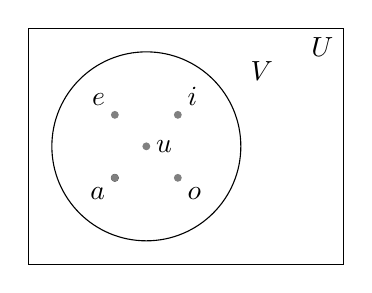
\begin{tikzpicture}
\fill[black] (-0.4,-0.4) circle (0.05cm);
\fill[gray] (-0.4,0.4) circle (0.05cm);
\fill[gray] (-0.4,-0.4) circle (0.05cm);
\fill[gray] (0.4,0.4) circle (0.05cm);
\fill[gray] (0.4,-0.4) circle (0.05cm);
\fill[gray] (0,0) circle (0.05cm);
\draw (0,0) circle (1.2cm);
\draw (-1.5,-1.5) rectangle (2.5,1.5) node [text=black,below left] {$U$};
\draw (-0.4,-0.4) node [text=black,below left] {$a$};
\draw (-0.4,0.4)  node [text=black,above left] {$e$};
\draw (0.4,0.4)   node [text=black,above right] {$i$};
\draw (0.4,-0.4)  node [text=black,below right] {$o$};
\draw (1.2,1.2)   node [text=black,below right] {$V$};
\draw (0,0)       node [text=black,right] {$u$};
\end{tikzpicture}
%\end{center}
\caption{Venn graph for the set of vowels.}
\label{fig1-001}       % Give a unique label
\end{figure}



It is common to encounter situations where the elements of one set are also the elements of
a second set. We now introduce some terminologies and notations to express such relationships
between sets.

\begin{definition}
The set $A$ is a subset of $B$ if and only if every element of $A$ is also an element of $B$. We use
the notation $A\subseteq{B}$ to indicate that $A$ is a subset of the set $B$.
\end{definition}


We see that $A\subseteq B$ if and only if the quantification

\[\forall x(x\in A\Rightarrow{x}\in{B})\]

\noindent is true. Note that to show that $A$ is not a subset of $B$ we need only find one element $x\in{A}$ with
$x\notin{B}$. Such an $x$ is a counterexample to the claim that $x\in{A}$ implies $x\in{B}$.


\begin{example}
The set of all odd positive integers less than 10 is a subset of the set of all positive integers less
than 10, the set of rational numbers is a subset of the set of real numbers, the set of all computer
science majors at your school is a subset of the set of all students at your school, and the set of
all people in China is a subset of the set of all people in China (that is, it is a subset of itself).
Each of these facts follows immediately by noting that an element that belongs to the first set
in each pair of sets also belongs to the second set in that pair.
\hfill$\square$
\end{example}



\begin{example}
The set of integers with squares less than 100 is not a subset of the set of nonnegative integers because -1 is in the former set (as $(-1)^2<100$), but not the later set. The set of people who
have taken discrete mathematics at your school is not a subset of the set of all computer science majors at your school if there is at least one student who has taken discrete mathematics who is
not a computer science major.
\hfill$\square$
\end{example}

Given any nonempty set $S$, it is guaranteed to have at least two subsets, the empty set and the set $S$ itself, that is, $\emptyset\subseteq{S}$ and $S\subseteq{S}$.

When we wish to emphasize that a set $A$ is a subset of a set $B$ but that $A\neq B$, we write
$A\subset{B}$ and say that $A$ is a \textit{proper subset} of $B$. For $A\subset{B}$ to be true, it must be the case that
$A\subseteq{B}$ and there must exist an element $x$ of $B$ that is not an element of $A$. That is, $A$ is a proper
subset of $B$ if and only if

\[\forall x(x\in{A}\Rightarrow x\in{B})\wedge\exists{y}(y\in{B}\wedge y\notin{A})\]


\noindent is true. Venn diagrams can be used to illustrate that a set $A$ is a subset of a set $B$. We draw the
universal set $U$ as a rectangle. Within this rectangle we draw a circle for $B$. Because $A$ is a subset
of $B$, we draw the circle for $A$ within the circle for $B$. This relationship is shown in Figure \ref{fig1-002}.



\begin{figure}[htbp]
%\sidecaption
%\includegraphics[scale=.45]{fig1-002.eps}
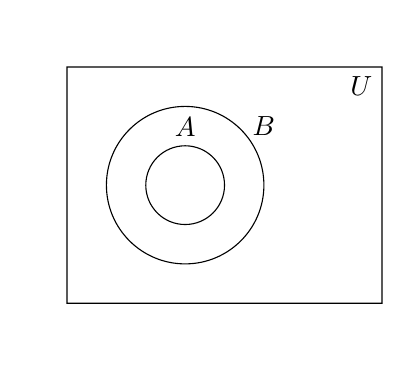
\begin{tikzpicture}[fill=gray]
% left hand
\scope
\clip (-2,-2) rectangle (2,2)
      (1,0) circle (1);
%\fill (0,0) circle (1);
\endscope
% right hand
\scope
\clip (-2,-2) rectangle (2,2)
      (0,0) circle (1);
%\fill (1,0) circle (1);
\endscope
% outline
%\fill[gray] (0,0) circle (0.5);
\draw (0,0) circle (0.5) (0,0.5)  node [text=black,above] {$A$}
      (0,0) circle (1) (1,1)  node [text=black,below] {$B$}
      (-1.5,-1.5) rectangle (2.5,1.5) node [text=black,below left] {$U$};
\end{tikzpicture}
\caption{Venn graph showing that $A$ is a proper subset of $B$.}
\label{fig1-002}       % Give a unique label
\end{figure}





A useful way to show that two sets have the same elements is to show that each set is a subset of the other. In other words, we can show that if $A$ and $B$ are sets with $A\subseteq{B}$ and $B\subseteq{A}$, then $A=B$. That is, $A=B$ if and only if $\forall x(x\in A\Rightarrow x\in{B})$ and $\forall x(x\in{B}\Rightarrow x\in A)$ or
equivalently if and only if $\forall x(x\in{A}\Leftrightarrow x\in{B})$, which is what it means for the $A$ and $B$ to be
equal.

\begin{example}
$A=\{\emptyset, \{a\}, \{b\}, \{a,b\}\}$ and $B=\{x|x~\text{is a subset of the set}~\{a,b\}\}$ are equal.
\hfill$\square$
\end{example}



\textbf{The Size of a Set}~~Sets are used extensively in counting problems, and for such applications we need to discuss
the sizes of sets.

\begin{definition}
Let $S$ be a set. If there are exactly $n$ distinct elements in $S$ where $n$ is a nonnegative integer,
we say that $S$ is a finite set and that $n$ is the cardinality of $S$. The cardinality of S is denoted by $|S|$.
\end{definition}


\begin{example}
Let $A$ be the set of odd positive integers less than 10. Then $|A|=5$. \hfill$\square$
\end{example}

\begin{example}
Let $S$ be the set of letters in the English alphabet. Then $|S|= 26$. \hfill$\square$
\end{example}



\begin{example}
Because the null set has no elements, it follows that $|\emptyset| =0$. \hfill$\square$
\end{example}

A set is said to be \textit{infinite} if it is not finite. For example, the set of all nonnegative integers $\{0, 1, 2, \ldots\}$ is infinite and the set of all even nonnegative numbers $\{0, 2, 4, \ldots\}$ is infinite. It is obvious that $\{0, 2, 4, \ldots\}$ is a proper subset of $\{0, 1, 2, \ldots\}$.
We will extend the notion of cardinality to infinite sets in Section 2.5, which is a challenging topic
full of surprising results \footnote{For a finite set, its cardinality provides an exact measure of its size. However, for infinite sets, the cardinality is a relative measure of two sets. Specifically, we can define what it means for one infinite set to have a small cardinality than another infinite set. The pertinent results regarding this issue are largely attributed to the work of Cantor and Julius Wilhelm Richard Dedekind (1831--1916). A primary surprising result is that sets $A=\{2, 4, 6, \ldots\}$ and $\mathbb{N}^+=\{1, 2, 3, \ldots\}$ have the same cardinality, represented by $|A|=|\mathbb{N}^+|$ (although $A\subset\mathbb{N}^+$ is obviously true). Since the concept of functions is needed to define the cardinality of an infinite set, we leave the problem in Chapter 2.}.


\textbf{Power Sets}~~Many problems involve testing all combinations of elements of a set to see if they satisfy some
property. To consider all such combinations of elements of a set $S$, we build a new set that has
as its members all the subsets of $S$.


\begin{definition}
Given a set $S$, the power set of $S$ is the set of all subsets of the set $S$. The power set of $S$ is
denoted by $\mathcal{P}(S)$.
\end{definition}



\begin{example}
The power set $\mathcal{P}(\{0, 1, 2\})$ is the set of all subsets of \{0, 1, 2\}. Hence,
$\mathcal{P}(\{0, 1, 2\})=\{\emptyset, \{0\}, \{1\}, \{2\}, \{0, 1\}, \{0, 2\}, \{1, 2\}, \{0, 1, 2\}\}$.
\hfill$\square$
\end{example}


\begin{example}
We have $\mathcal{P}(\emptyset)=\{\emptyset\}$ and $\mathcal{P}(\{\emptyset\})=\{\emptyset, \{\emptyset\}\}$.
\hfill$\square$
\end{example}

\begin{remark}
If a set $A$ has $n$ (disctinct) elements, then its power set contains $2^n$ members. Accordingly, sometimes $\mathcal{P}$ is written as $2^A$. \hfill$\square$
\footnote{\parpic{\includegraphics[width=2.0cm]{Dedekind.eps}}\noindent Julius Wilhelm Richard Dedekind (1831--1916) was a German mathematician who made important contributions to abstract algebra (particularly ring theory), algebraic number theory and the definition of the real numbers.\\
He was born, lived most of his life, and died in Braunschweig (often called ``Brunswick'' in English).
He first attended the Collegium Carolinum in 1848 before transferring to the University of G\"{o}ttingen in 1850. There, Dedekind was taught number theory by Professor Moritz Stern and he became Gauss's last student there. Dedekind received his doctorate in 1852. The thesis however did not display the talent evident by his subsequent work.\\
Dedekind went to Berlin for two years of study, where he and Bernhard Riemann (1826--1866, a German mathematician who made contributions to analysis, number theory, and differential geometry) were contemporaries; they were both awarded the habilitation in 1854. Dedekind returned to G\"{o}ttingen to teach, giving courses on probability and geometry. He studied for a while with Peter Gustav Lejeune Dirichlet (1805--1859, a German mathematician who made deep contributions to number theory, Fourier series and other topics in mathematical analysis, credited with being one of the first mathematicians to give the modern formal definition of a function), and they became good friends.
\\
Dedekind developed the notion now known as a Dedekind cut, now a standard definition of the real numbers.
In 1888, he published a short monograph titled ``What are numbers and what should they be?'' which included his definition of an infinite set. He also proposed an axiomatic foundation for the natural numbers, whose primitive notions were the number one and the successor function. In 1872, while on holiday in Interlaken, Dedekind met Georg Cantor. Thus they began an enduring relationship of mutual respect, and Dedekind became one of the very first mathematicians to admire Cantor's work concerning infinite sets, proving a valued ally in Cantor's disputes with Leopold Kronecker, who was philosophically opposed to Cantors's transfinite numbers.\\
He retired in 1894, but did occasional teaching and continued to publish. He never married, instead living with his sister Julia.
Dedekind was elected to the Academies of Berlin (1880) and Rome, and to the French Academy of Sciences (1900). He received honorary doctorates from the universities of Oslo, Zurich, and Braunschweig.\\
Interestingly and accidentally, Johann Carl Friedrich Gauss (1777--1855, a German mathematician who contributed significantly to many fields, including number theory, algebra, statistics, analysis, differential geometry, geodesy, geophysics, mechanics, electrostatics, astronomy, matrix theory, and optics, referred to as ``the foremost of mathematicians'' and ``greatest mathematician since antiquity''. Gauss had an exceptional influence in many fields of mathematics and science and is ranked as one of history's most influential mathematicians) was also born in the small town Braunschweig (252,768 people, as of 31 December 2015), where the residents are all proud of the two mathematicians.\\
There is an anecdote regarding the death of Dedekind. He lived so long that although some of his work had been familiar to all the students of analysis for a generation before his death, he himself had become almost a legend and many classed him with the shadowy dead. Twelve years before his death, a book \textit{Calendar for Mathematicians} listed Dedekind as having died on September 4, 1899, much to Dedekind's amusement. The day, September 4, might possible prove to be correct, he wrote to the editor of the book, but the year was certainly wrong.  `According to my memorandum I passed this day in perfect health and enjoyed a very stimulating conversation on ``system and theory'' with my luncheon guest and honoured friend Georg Cantor of Halle.'}
\end{remark}

\begin{remark}
For a finite non-empty set $A$, it is rather intuitive that the cardinality of set $A$ is strictly less than that of its power set $2^A$ or $\mathcal{P}(A)$, i.e., $|A|<|\mathcal{P}(A)|$. When $A$ is infinite, $\mathcal{P}(A)$ is naturally infinite. The relative measure of $|A|$ and $|\mathcal{P}(A)|$ is important for mathematics analysis. \hfill$\square$
\end{remark}


\textbf{Cartesian Products}~~The order of elements in a collection is often important. Because sets are unordered, a different
structure is needed to represent ordered collections. This is provided by \textbf{ordered $n$-tuples}.

\begin{definition}
An ordered $n$-tuple $(a_1, a_2, \ldots, a_n)$ is the ordered collection that has $a_1$ as its first element,
$a_2$ as its second element, $\ldots$, and $a_n$ as its $n$-th element.
\end{definition}

We say that two ordered $n$-tuples are equal if and only if each corresponding pair of their
elements is equal. In other words, $(a_1, a_2, \ldots, a_n)=(b_1, b_2, \ldots, b_n)$ if and only if $a_i=b_i$,
for $i=1, 2, \ldots, n$. In particular, ordered 2-tuples are called ordered pairs. The ordered pairs
$(a, b)$ and $(c, d)$ are equal if and only if $a=c$ and $b=d$. Note that $(a, b)$ and $(b, a)$ are not
equal unless $a=b$.

Many of the discrete structures are based on the notion of the
Cartesian product of sets (named after Ren\'{e} Descartes). We first define the Cartesian product
of two sets \footnote{\parpic{\includegraphics[width=2cm]{Descartes.eps}}\noindent Ren\'{e} Descartes (1596--1650) was a French philosopher, mathematician, and scientist. Dubbed the father of modern western philosophy, much of subsequent Western philosophy is a response to his writings, which are studied closely to this day.\\
Descartes was born into a noble family near Tours, France, about
200 miles southwest of Paris. He was the third child of his father's first wife. When he was one year old, his mother Jeanne Brochard died after trying to give birth to another child who also died. Because of Ren\'{e}'s poor health, his father, a provincial judge, let his son's formal lessons slide until, at
the age of 8, Ren\'{e} entered the Jesuit college at La Fl\`{e}che. The rector of the school took a liking to him and
permitted him to stay in bed until late in the morning because of his frail health. From then on, Descartes spent
his mornings in bed; he considered these times his most productive hours for thinking.\\
Descartes left school in 1612, moving to Paris, where he spent 2 years studying mathematics. He earned
a law degree in 1616 from the University of Poitiers. At 18 Descartes became disgusted with studying and
decided to see the world. He moved to Paris and became a successful gambler. However, he grew tired
of bawdy living and moved to the suburb of Saint-Germain, where he devoted himself to mathematical study. When his gambling
friends found him, he decided to leave France and undertake a military career. However, he never did any fighting. One day, while
escaping the cold in an overheated room at a military encampment, he had several feverish dreams, which revealed his future career as a mathematician and philosopher.\\
After ending his military career, he traveled throughout Europe. He then spent several years in Paris, where he studied mathematics and philosophy and constructed optical instruments. Descartes decided to move to Holland, where he spent 20 years wandering around the country, accomplishing his most important work. During this time he wrote several books, including the \textit{Discours}, which contains his contributions to analytic geometry, for which he is best known. He also made fundamental contributions to philosophy. \\
In 1649 Descartes was invited by Queen Christina to visit her court in Sweden to tutor her in philosophy. Although he was
reluctant to live in what he called ��the land of bears amongst rocks and ice,�� he finally accepted the invitation and moved to Sweden. Unfortunately, the winter of 1649--1650 was extremely bitter. Descartes caught pneumonia and died in mid-February.\\
One of Descartes' most enduring legacies was his development of Cartesian or analytic geometry, which uses algebra to describe geometry. He invented the convention of representing unknowns in equations by $x$, $y$, and $z$, and knowns by $a$, $b$, and $c$. He also pioneered the standard notation that uses superscripts to show the powers or exponents, e.g., $x^3$.
\\Current opinion is that Descartes had the most influence of anyone on the young Newton, and this is arguably one of Descartes' most important contributions. Newton continued Descartes' work on cubic equations, which freed the subject from the fetters of the Greek perspectives. Descartes' work provided the basis for the \textit{calculus} developed by Isaac Newton (1642--1726) and Gottfried Leibniz (1646--1716), who applied infinitesimal calculus to the tangent line problem, thus permitting the evolution of that branch of modern mathematics.}.



\begin{definition}
Let $A$ and $B$ be sets. The Cartesian product of $A$ and $B$, denoted by $A\times{B}$, is the set of all
ordered pairs $(a, b)$, where $a\in{A}$ and $b\in{B}$, i.e.,

\[A\times{B}=\{(a, b)|a\in A\wedge b\in B\}.\]
\end{definition}


\begin{example}
Let $A$ represent the set of all students at a university, and let $B$ represent the set of all courses
offered at the university. The Cartesian product $A\times{B}$ consists of all the ordered pairs of the form $(a, b)$, where
$a$ is a student at the university and $b$ is a course offered at the university. One way to use the set
$A\times{B}$ is to represent all possible enrollments of students in courses at the university.
\hfill$\square$
\end{example}


\begin{example}
Let $A=\{1, 2\}$ and $B=\{a, b, c\}$. The Cartesian product $A\times{B}$ is
$A\times{B}=\{(1, a), (1, b), (1, c), (2, a), (2, b), (2, c)\}$.
\hfill$\square$
\end{example}


If any of $A$ and $B$ is empty, $A\times{B}=B\times{A}=\emptyset$. However, in general, $A\times{B}\neq{B\times{A}}$ unless $A=B$. The Cartesian product of more than two sets can also be defined.

\begin{definition}
The Cartesian product of the sets $A_1$, $A_2$, $\ldots$, $A_n$, denoted by $A_1\times{A_2}\times\ldots\times{A_n}$, is the
set of ordered $n$-tuples $(a_1, a_2, \ldots, a_n)$, where $a_i$ belongs to $A_i$ for $i=1, 2, \ldots, n$. In other
words,

\[A_1\times A_2\times\ldots\times A_n=\{(a_1, a_2, \ldots, a_n)|a_i\in A_i~\text{for}~i=1,2, \ldots, n\}.\]
\end{definition}


\begin{example}
Let $A=\{0, 1\}, B=\{1, 2\}$, and $C=\{0, 1, 2\}$. $A\times{B}\times{C}$ consists of all ordered triples $(a, b, c)$, where $a\in{A}$, $b\in{B}$, and $c\in{C}$. Hence,

$A\times{B}\times{C}=\{(0, 1, 0), (0, 1, 1), (0, 1, 2), (0, 2, 0), (0, 2, 1), (0, 2, 2)$, $(1$, $1$, $0)$, $(1$, $1$, $1)$, $(1$, $1, 2), (1, 2, 0), (1, 2, 1), (1, 2, 2)\}.$
\hfill$\square$
\end{example}


We use the notation $A^2$ to denote $A\times{A}$, the Cartesian product of the set $A$ with itself.
Similarly, $A^3=A\times{A}\times{A}$, $A^4=A\times{A}\times{A}\times{A}\times{A}$, and so on. More generally,

\[A^n =\{(a_1, a_2, \ldots, a_n) | a_i\in A~\text{for}~i=1, 2, \ldots, n\}.\]


\begin{example}
Let $A=\{1, 2\}$ be a set. It follows that $A^2=\{(1, 1), (1, 2), (2, 1), (2, 2)\}$ and $A^3=\{(1, 1, 1), (1, 1, 2), (1, 2, 1), (1, 2, 2), (2, 1, 1), (2, 1, 2), (2, 2, 1), (2, 2, 2)\}$.
\hfill$\square$
\end{example}


A subset $R$ of the Cartesian product $A\times{B}$ is called a relation \footnote{\textit{Relation} is an important concept in discrete mathematics, which will be introduced in Chapter 3.} from the set $A$ to the set
$B$. The elements of $R$ are ordered pairs, where the first element belongs to $A$ and the second
to $B$. For example, $R=\{(a, 0), (a, 1), (a, 3), (b, 1), (b, 2), (c, 0), (c, 3)\}$ is a relation from the
set $\{a, b, c\}$ to the set $\{0, 1, 2, 3\}$. A relation from a set $A$ to itself is called a relation on $A$.


Suppose that $A$=\{G88\} and $B$=\{Xian, Zhengzhou, Hebi, Xingtai, Shijiazhuang, Baoding, Beijing\}. Then $R$=\{(G88, Xian), (G88, Zhengzhou), (G88, Shijiazhuang), (G88, Beijing)\} is a relation from $A$ to $B$, indicating the cites in which High Speed Rail G88 (China Railway Corporation) stops over.

\begin{example}
Let $A=\{0,1,2,3\}$ and $R=\{(a,b)|a\leq{b}\}$ be a relation on $A$. Then
$R=\{(0,0)$, $(0,1), (0,2), (0,3), (1,1), (1,2), (1,3),
(2,2), (2, 3), (3, 3)\}$. \hfill$\square$
\end{example}

\section{Set Operations}

Two, or more, sets can be combined in many different ways. For instance, starting with the set
of mathematics majors at your school and the set of computer science majors at your school, we
can form the set of students who are mathematics majors or computer science majors, the set of
students who are joint majors in mathematics and computer science, the set of all students not
majoring in mathematics, and so on.

\begin{definition}
Let $A$ and $B$ be sets. The union of the sets $A$ and $B$, denoted by $A\cup{B}$, is the set that contains
those elements that are either in $A$ or in $B$, or in both.
\end{definition}

An element $x$ belongs to the union of the sets $A$ and $B$ if and only if $x$ belongs to $A$ or $x$ belongs
to $B$. This tells us that

\[A\cup B=\{x|x\in{A}\vee x\in{B}\}.\]


The Venn diagram shown in Figure \ref{union of two sets} represents the union of two sets $A$ and $B$. The area
that represents $A\cup{B}$ is the shaded area within either the circle representing $A$ or the circle
representing $B$.

\begin{figure}[htbp]
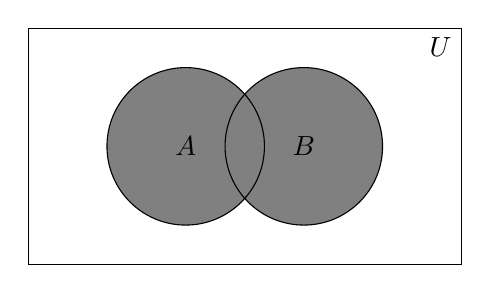
\begin{tikzpicture}
\draw (-2,-1.5) rectangle (3.5,1.5) node[below left]{$U$};
\fill[gray] (0,0) circle (1cm);
\fill[gray] (1.5,0) circle (1cm);
\draw (0,0) circle (1cm) node {$A$};
\draw (1.5,0) circle (1cm) node {$B$};
\end{tikzpicture}
\caption{Venn graph of the union of two sets.}
\label{union of two sets}
\end{figure}

\begin{example}
The union of the sets \{1, 3, 5\} and \{1, 2, 3\} is the set \{1, 2, 3, 5\}; that is,
\{1, 3, 5\}$\cup$\{1, 2, 3\}=\{1, 2, 3, 5\}.
\hfill$\square$
\end{example}


\begin{example}
The union of the sets $\{a, b, c, d\}$ and $\{1, 2, b, d, e\}$ is the set $\{1$, $2$, $a$, $b$, $c$, $d$, $e\}$.
\hfill$\square$
\end{example}

\begin{example}
The union of the set of all computer science majors at Xidian University and the set of all mathematics
majors at Xidian University is the set of students at Xidian University who are majoring either in
mathematics or in computer science (or in both).
\hfill$\square$
\end{example}


\begin{definition}
Let $A$ and $B$ be sets. The \textit{intersection} of the sets $A$ and $B$, denoted by $A\cap{B}$, is the set
containing those elements in both $A$ and $B$.
\end{definition}

An element $x$ belongs to the intersection of the sets $A$ and $B$ if and only if $x$ belongs to $A$ and
$x$ belongs to $B$. This tells us that

\[A\cap{B}=\{x|x\in A\wedge x\in B\}.\]



The Venn diagram shown in Figure \ref{intersection of two sets} represents the intersection of two sets $A$ and $B$. The shaded
area that is within both the circles representing the sets $A$ and $B$ is the area that represents the
intersection of $A$ and $B$.

\begin{figure}[htbp]
%\begin{center}
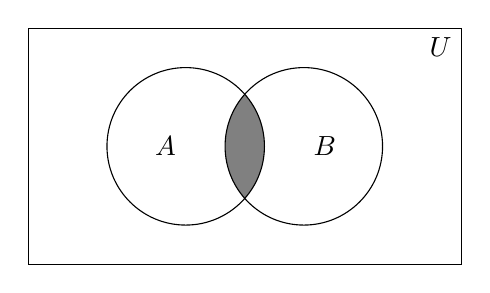
\begin{tikzpicture}
\draw (-2,-1.5) rectangle (3.5,1.5) node[below left]{$U$};
\begin{scope} % start of clip scope
\clip (0,0) circle (1cm);
\fill[gray] (1.5,0) circle (1cm);
\end{scope} % end of clip scope
\draw (0,0) circle (1cm) node[left] {$A$};
\draw (1.5,0) circle (1cm) node[right] {$B$};
\end{tikzpicture}
%\end{center}
\caption{Venn graph of the intersection of two sets.}
\label{intersection of two sets}
\end{figure}


\begin{example}
The intersection of the sets \{1, 3, 5\} and \{1, 2, 3\} is the set \{1, 3\}; that is,
$\{1, 3, 5\}\cap\{1, 2, 3\} = \{1, 3\}$.
\hfill$\square$
\end{example}


\begin{example}
The intersection of the set of all computer science majors at your school and the set of all
mathematics majors is the set of all students who are joint majors in mathematics and computer
science.
\hfill$\square$
\end{example}



We are often interested in finding the cardinality of a union of two finite sets $A$ and $B$. Note that $|A|+|B|$ counts each element that is in $A$ but not in $B$ or in $B$ but not in $A$ exactly once, and each element that is in both $A$ and $B$ exactly twice. Thus, if the number of elements that
are in both $A$ and $B$ is subtracted from $|A|+|B|$, elements in $A\cap B$ will be counted only once. Hence,

\[|A\cup B|=|A|+|B|-|A\cap B|.\]


\begin{definition}
Two sets are said to be \textit{disjoint} if their intersection is the empty set.
\hfill$\square$
\end{definition}


\begin{example}
Let $A=\{1, 3, 5, 7, 9\}$ and $B=\{2, 4, 6, 8, 10\}$. Because $A\cap B=\emptyset$, $A$ and $B$ are disjoint.
\hfill$\square$
\end{example}


\begin{definition}
Let $A$ and $B$ be sets. The \textit{difference} of $A$ and $B$, denoted by $A-B$ or $A\setminus{B}$, is the set containing those
elements that are in $A$ but not in $B$. The difference of $A$ and $B$ is also called the \textit{complement} of $B$ with respect to $A$.
\end{definition}

An element $x$ belongs to the difference of $A$ and $B$ if and only if $x\in A$ and $x\notin{B}$. This tells us
that

\[A-B=\{x|x\in A\wedge x\notin B\}.\]


The Venn diagram shown in Figure \ref{Difference of two sets} represents the difference of the sets $A$ and $B$. The shaded
area inside the circle that represents $A$ and outside the circle that represents $B$ is the area that
represents $A-B$.


\begin{figure}[htbp]
%\begin{center}
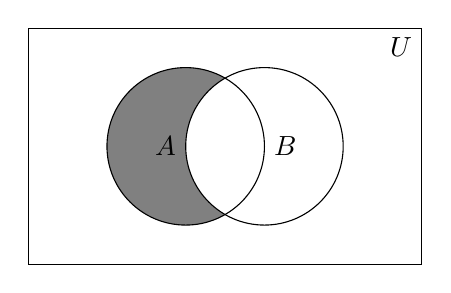
\begin{tikzpicture}
\draw (-2,-1.5) rectangle (3,1.5) node[below left]{$U$}; % draw a rectangle
\fill[gray] (0,0) circle (1cm); % then fill in a circular region
\fill[white] (1,0) circle (1cm); % then fill in a 2nd circular region
\draw (0,0) circle (1cm) node[left] {$A$};
\draw (1,0) circle (1cm) node[right] {$B$};
\end{tikzpicture}
%\end{center}
\caption{Venn graph of the difference of two sets.}
\label{Difference of two sets}
\end{figure}


\begin{example}
The difference of \{1, 3, 5\} and \{1, 2, 3\} is the set \{5\}; that is, $\{1, 3, 5\}-\{1, 2, 3\}=\{5\}$. This
is different from the difference of \{1, 2, 3\} and \{1, 3, 5\}, which is the set \{2\}.
\hfill$\square$
\end{example}

\begin{example}
The difference of the set of computer science majors at your school and the set of mathematics majors at your school is the set of all computer science majors at your school who are not also
mathematics majors.
\hfill$\square$
\end{example}



Once the universal set $U$ has been specified, the complement of a set can be defined.


\begin{definition}
Let $U$ be the universal set. The \textit{complement} of the set $A$, denoted by $\overline{A}$, is the complement
of $A$ with respect to $U$. Therefore, the complement of the set A is $U-A$.
\end{definition}

An element belongs to $\overline{A}$ if and only if $x\notin{A}$. This tells us that

\[\overline{A}=\{x\in U|x\notin A\}.\]


In Figure \ref{complement of a set} the shaded area outside the circle representing $A$ is the area representing $\overline{A}$.

\begin{figure}[htbp]
\begin{center}
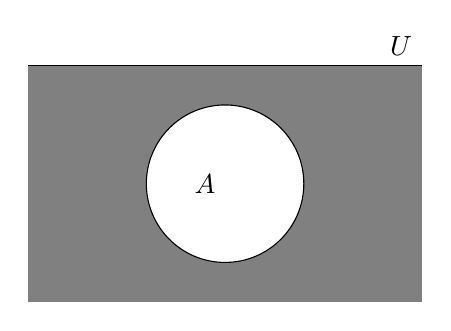
\begin{tikzpicture}
\draw (-2,-1.5) rectangle (3,1.5) node[above left] {$U$}; % draw a rectangle
\fill[gray] (-2,-1.5) rectangle (3,1.5); % then fill in a circular region
\fill[white] (0.5,0) circle (1cm); % then fill in a 2nd circular region
\draw (0.5,0) circle (1cm) node[left] {$A$};
\end{tikzpicture}
\caption{Venn diagram of the complement of a set.}
\label{complement of a set}
\end{center}
\end{figure}

\begin{example}
Let $A=\{a, e, i, o, u\}$ (where the universal set is the set of letters of the English alphabet). Then
$\overline{A}=\{b, c, d, f, g, h, j, k, l, m, n, p, q, r, s, t, v, w, x, y, z\}$.
\hfill$\square$
\end{example}


\begin{example}
Let $A$ be the set of positive integers greater than 10 (with universal set the set of all positive
integers). Then $\overline{A}=\{1, 2, 3, 4, 5, 6, 7, 8, 9, 10\}$.
\hfill$\square$
\end{example}


\textbf{Set Identities}~~
Table \ref{set identities} lists the most important set identities. We can prove these identities
using different methods. These methods are presented to illustrate that there are often many
different approaches to the solution of a problem. The proofs of the remaining identities will
\marginpar{\small Set identities and propositional equivalences are just special cases of identities
for Boolean algebra.}
be left as exercises. The reader should note the similarity between these set identities and the
logical equivalences. In fact, the set identities given can be proved directly from the corresponding logical equivalences.
Furthermore, both are special cases of identities that hold for Boolean algebra.

\begin{table}
\caption{Set identities}
\begin{tabular}{|p{8cm}||p{3cm}|}
  \hline
  Identity & Name\\
  \hline
  $A\cap{U}=A$, $A\cup\emptyset=A$ & Identity laws \\
  \hline
  $A\cup{U}=U$, $A\cap\emptyset=\emptyset$ & Domination laws \\
  \hline
  $A\cup{A}=A$, $A\cap{A}=A$ & Idempotent laws \\
  \hline
  $\overline{(\overline{A})}=A$ & Complementation law \\
  \hline
  $A\cup{B}=B\cup{A}$, $A\cap{B}=B\cap{A}$ & Commutative laws \\
  \hline
  $A\cup{(B\cup C)}=(A\cup B)\cup{C}$, $A\cap{(B\cap C)}=(A\cap{B})\cap{C}$ & Associative laws \\
  \hline
  $A\cup(B\cap C)=(A\cup B)\cap(A\cup C)$, $A\cap (B\cup C)=(A\cap B)\cup(A\cap C)$ & Distributive laws \\
  \hline
  $\overline{A\cap B}=\overline{A}\cup\overline{B}$, $\overline{A\cup{B}}=\overline{A}\cap\overline{B}$ & De Morgan's laws\\
    \hline
  $A\cup(A\cap B)=A$, $A\cap(A\cup B)=A$ & Absorption laws \\
  \hline
  $A\cup\overline{A}=U$, $A\cap\overline{A}=\emptyset$ & Complement laws \\
  \hline
\end{tabular}
\label{set identities}
\end{table}

One way to show that two sets are equal is to show that each is a subset of the other. Recall
that to show that one set is a subset of a second set, we can show that if an element belongs to
the first set, then it must also belong to the second set. We generally use a direct proof to do this.
We illustrate this type of proof by establishing the first of De Morgan's laws.



\begin{example}
Prove that $\overline{(A\cap B)}=\overline{A}\cup\overline{B}$.

Solution: First, we will show that $\overline{A\cap B}\subseteq\overline{A}\cup\overline{B}$. We do this by showing that if $x$ is in $\overline{A\cap B}$, then it must also be in $\overline{A}\cup\overline{B}$. Now suppose that $x\in\overline{A\cap B}$. By the definition of complement, $x\notin A\cap B$. Using the definition of intersection, we see that the proposition $\neg((x\in A) \wedge(x\in B))$ is true.

By applying De Morgan's law for propositions, we see that $\neg(x\in A)$ or $\neg(x\in B)$. Using
the definition of negation of propositions, we have $x\notin A$ or $x\notin B$. Using the definition of
the complement of a set, we see that this implies that $x\in\overline{A}$ or $x\in\overline{B}$. Consequently, by the
definition of union, we see that $x\in\overline{A}\cup\overline{B}$. We have now shown that $\overline{A\cap B}\subseteq\overline{A}\cup\overline{B}$.

Next, we will show that $\overline{A}\cup\overline{B}\subseteq\overline{A\cap B}$. We do this by showing that if $x$ is in $\overline{A}\cup\overline{B}$, then it must also be in $\overline{A\cap B}$. Now suppose that $x\in\overline{A}\cup\overline{B}$. By the definition of union, we know that
$x\in\overline{A}$ or $x\in\overline{B}$. Using the definition of complement, we see that $x\notin A$ or $x\notin B$. Consequently, the proposition $\neg(x\in A)\vee\neg(x\in B)$ is true.

By De Morgan's law for propositions, we conclude that $\neg((x\in A)\wedge(x\in B))$ is true.
By the definition of intersection, it follows that $\neg(x\in A\cap B)$. We now use the definition of
complement to conclude that $x\in\overline{A\cap B}$. This shows that $\overline{A}\cup\overline{B}\subseteq\overline{A\cap B}$.

Because we have shown that each set is a subset of the other, the two sets are equal, and the identity is proved. \marginpar{\small Mathematical induction, a form of direct proof, is a mathematical proof technique used to prove a given statement about any well-ordered set.} \footnote{\parpic{\includegraphics[width=2.0cm]{Morgan.eps}}Augustus De Morgan (1806--1871) was a British mathematician and logician. He formulated De Morgan's laws and introduced the term mathematical induction, making its idea rigorous. In his own time he was better known as a newspaper columnist.\\
De Morgan studied at Trinity College, Cambridge, graduating in 1827. Although he considered medicine or law, he decided on
mathematics for his career. In the 1840s De Morgan made fundamental contributions to the development of symbolic logic. He invented notations that helped him prove propositional equivalences, such as the laws that are named after him. In 1842 De Morgan presented what is considered to be the first precise definition of a limit and developed new tests for convergence of infinite series. De Morgan was also interested in the history of mathematics and wrote biographies of \underline{Newton} and \underline{Halley} (1656--1742, an English astronomer, geophysicist, mathematician, meteorologist, and physicist who is best known for computing the orbit of Halley's Comet).
\\
De Morgan was famous for his opposition to negative numbers, which nowadays flabbergasts our contemporaries since, without thinking too much about it, most of us can use negative numbers for things like recording temperatures below zero and representing economy recession by negative increase. It takes a long time until the end of the 19th century that negative numbers are well accepted by the community of mathematics as part of the number system. \\
Although the first set of rules for dealing with negative numbers was stated in the 7th century by the Indian mathematician Brahmagupta, it is surprising that in 1758 the British mathematician \underline{Francis Maseres} (1731--1824, an English lawyer, known as attorney general of the Province of Quebec, judge, mathematician, historian, and member of the Royal Society) was claiming that negative numbers\\
``\ldots\ldots darken the very whole doctrines of the equations and make dark of the things which are in their nature excessively obvious and simple''.\\
In the early work solving equations, negative roots were not even considered. Hindu mathematicians in the sixth century, and before that, Chinese mathematicians figured out all the rules for operations with negative numbers. Yet the Arabs did not include any of this in their work three centuries later. French mathematician \underline{Blaise Pascal} (1623-1662, a French mathematician, physicist, inventor, writer and Catholic theologian) did not see the need for negative numbers. De Morgan thought numbers less than zero were unimaginable. \\For females, De Morgan cautioned them against
studying too much mathematics, because it might interfere with their childbearing abilities.}
\hfill$\square$
\label{set identity 1}
\end{example}


We can more succinctly express the reasoning used in Example \ref{set identity 1} using set builder notation,
as Example \ref{set identity 2} illustrates

\begin{example}
Use set builder notation and logical equivalences to establish the first De Morgan law $\overline{A\cap B}=
\overline{A}\cup\overline{B}$.

Solution: We can prove this identity with the following steps.

$\overline{A\cap{B}}=\{x|x\notin A\cap{B}\}$ \hfill by definition of complement

$=\{x|\neg(x\in(A\cap B))\}$ \hfill by definition of ``does not belong symbol''

$=\{x|\neg(x\in A\wedge x\in B)\}$ \hfill by definition of intersection

$=\{x |\neg(x\in A)\vee\neg(x\in B)\}$ \hfill by the second De Morgan law

\hfill for logical equivalences
\marginpar{De Morgan's law for logical equivalence is $\neg(p\wedge q)=\neg p\vee\neg q$ and $\neg(p\vee q)=\neg p\wedge\neg q$, where $p$ and $q$ are propositions.}


$=\{x|x\notin A\vee\notin B\}$ \hfill by definition of ``does not belong symbol''

$=\{x|x\in\overline{A}\vee x\in\overline B\}$ \hfill by definition of complement

$=\{x|x\in\overline{A}\cup\overline{B}\}$ \hfill by definition of union

$=\overline{A}\cup\overline{B}$ \hfill by meaning of set builder notation

Note that besides the definitions of complement, union, set membership, and set builder
notation, this proof uses the second De Morgan law for logical equivalences.
\hfill$\square$
\label{set identity 2}
\end{example}


\begin{example}
Prove the second distributive law from Table 1, which states that
$A\cap (B\cup C)=(A\cap B)\cup (A\cap C)$ for all sets $A$, $B$, and $C$.


Solution: We will prove this identity by showing that each side is a subset of the other side.
Suppose that $x\in A\cap(B\cup C)$. Then $x\in A$ and $x\in B\cup C$. By the definition of union, it
follows that $x\in A$, and $x\in B$ or $x\in C$ (or both). In other words, we know that the compound
proposition $(x\in A)wedge((x\in B)\vee(x\in C))$ is true. By the distributive law for conjunction over
disjunction, it follows that $((x\in A)\wedge(x\in B))\vee((x\in A)\wedge(x\in C))$. We conclude that either
$x\in A$ and $x\in B$, or $x\in A$ and $x\in C$. By the definition of intersection, it follows that $x\in A\cap B$
or $x\in A\cap C$. Using the definition of union, we conclude that $x\in (A\cap B)\cup(A\cap C)$. We
conclude that $A\cap(B\cup C)\subseteq(A\cap B)\cup(A\cap C)$.


Now suppose that $x\in(A\cap B)\cup(A\cap C)$. Then, by the definition of union, $x\in A\cap B$ or
$x\in A\cap C$. By the definition of intersection, it follows that $x\in A$ and $x\in B$ or that $x\in A$ and
$x\in C$. From this we see that $x\in A$, and $x\in B$ or $x\in C$. Consequently, by the definition of
union we see that $x\in A$ and $x\in B\cup C$. Furthermore, by the definition of intersection, it follows
that $x\in A\cap (B\cup C)$. We conclude that $(A\cap B)\cup(A\cap C)\subseteq A\cap(B\cup C)$. This completes
the proof of the identity.
\hfill$\square$
\end{example}


Because unions and intersections of sets satisfy associative laws, the sets $A\cup B\cup C$ and
$A\cap B\cap C$ are well defined; that is, the meaning of this notation is unambiguous when $A$,
$B$, and $C$ are sets. That is, we do not have to use parentheses to indicate which operation
comes first because $A\cup(B\cup C)=(A\cup B)\cup C$ and $A\cap(B\cap C)=(A\cap B)\cap C$. Note that
$A\cup B\cup C$ contains those elements that are in at least one of the sets $A$, $B$, and $C$, and that
$A\cap B\cap C$ contains those elements that are in all of $A$, $B$, and $C$.


\begin{example}
Let $A=\{0, 2, 4, 6, 8\}$, $B=\{0, 1, 2, 3, 4\}$, and $C=\{0, 3, 6, 9\}$. The set $A\cup B\cup C$ contains those elements in at least one of $A$, $B$, and $C$. Hence, $A\cup B\cup C=\{0, 1, 2, 3, 4, 6, 8, 9\}$.
The set $A\cap B\cap C$ contains those elements in all three of $A$, $B$, and $C$. Thus, $A\cap B\cap C=\{0\}$.
\hfill$\square$
\end{example}




\begin{definition}
The union of a collection of sets is the set that contains those elements that are members of
at least one set in the collection.
\end{definition}

We use the notation

\[A_1\cup A_2\cup\ldots\cup A_n=\cup_{i=1}^{n}A_i\]

\noindent to denote the union of the sets $A_1$, $A_2$, $\ldots$, $A_n$.

\begin{definition}
The intersection of a collection of sets is the set that contains those elements that are members
of all the sets in the collection.
\end{definition}

We use the notation

\[A_1\cap A_2\cap\ldots\cap A_n=\cap_{i=1}^{n}A_i\]

\noindent to denote the intersection of the sets $A_1$, $A_2$, $\ldots$, $A_n$.


\begin{example}
For $i=1, 2, \ldots$, let $A_i=\{i, i + 1, i + 2, \ldots\}$. Then,


\[\cup_{i=1}^{n}A_i=\cup_{i=1}^{n}\{i, i+1, i+2, \ldots\}=\{1, 2, 3, \ldots\},\]

and

\[\cap_{i=1}^{n}A_i=\cap_{i=1}^{n}\{i, i+1, i+2, \ldots\}=\{n, n+1, n+2, \ldots\}=A_n.\]
\hfill$\square$
\end{example}


\begin{definition}
Let $A_1$, $A_2$, $\ldots$, $A_n$ be subsets of $S$. $A_1$, $A_2$, $\ldots$, $A_n$ are said to be a partition of $S$ if (1) $\cup_{i=1}^{n}A_i=S$ and (2) $\forall i\neq{j}$ $(i,j\in\mathbb{N}_n)$, $A_i\cap{A_j}=\emptyset$.
\end{definition}



\begin{example}
Consider the following collections of subsets of $S=\{1, 2, . . ., 8, 9\}$:

(i) \{1, 3, 5\}, \{2, 6\}, \{4, 8, 9\};

(ii) \{1, 3, 5\}, \{2, 4, 6, 8\}, \{5, 7, 9\}; and

(iii) \{1, 3, 5\}, \{2, 4, 6, 8\}, \{7, 9\}.

It is trivial that (i) and (ii) are not the partition of $S$, while (iii) is.
\hfill$\square$
\end{example}

\section{Multi-sets}

In mathematics, a \textit{multiset} (or \textit{bag}) is a generalization of the concept of a set that, unlike a set, allows multiple instances of the multiset's elements. For example, $\{a, a, b\}$ and $\{a, b\}$ are different multisets although they are the same set. However, the order in a multiset does not matter. Specifically, $\{a, a, b\}$ and $\{a, b, a\}$ are the same multiset.


\underline{De~Bruijn}\footnote{\parpic{\includegraphics[width=2.0cm]{Bruijn.eps}}\noindent Nicolaas Govert de Bruijn (1918--2012) was a Dutch mathematician, noted for his many contributions in the fields of analysis, number theory, combinatorics and logic. De Bruijn started his academic career as at the University of Amsterdam, where he was Professor of Mathematics from 1952 to 1960. In 1960 he moved to the Technical University Eindhoven where he was Professor of Mathematics until his retirement in 1984.
In 1957 he was appointed member of the Royal Netherlands Academy of Arts and Sciences. He was Knighted with the Order of the Netherlands Lion.} coined the word \textit{multiset} in the 1970s. However, the use of multisets predates the word multiset by many centuries. The first study of multisets is usually attributed to an Indian mathematician who described permutations of multisets around 1150. In history, other names that were proposed or used for multisets include \textit{list}, \textit{bunch}, \textit{bag}, \textit{heap}, \textit{sample}, \textit{weighted set}, \textit{collection}, and \textit{suite}. The word ``visa'' is also used.

In the explicit form, multisets appeared in the work of \underline{Richard Dedekind}. Other mathematicians formalized multisets and began to study them as a precise mathematical object (structure) in the 20th century.

The multiplicity of an element is the number of instances of the element in a specific multiset. For example, an infinite number of multisets exist which contain only elements $a$ and $b$, varying only by multiplicity: The unique set $\{a, b\}$ contains only elements $a$ and $b$, each having multiplicity 1. In multiset $\{a, a, b\}$, $a$ has multiplicity 2 and $b$ has multiplicity 1.
In multiset $\{a, a, a, b, b, b\}$, $a$ and $b$ both have multiplicity 3.

\begin{definition}
Let $A$ be an ordinary set. A multiset $\alpha$ is a mapping from $A$ to $\mathbb{N}$ that gives the multiplicity of an element $a\in{A}$, denoted by $\alpha(a)$, representing the number of appearances of an element $a$ in $\alpha$. The cardinality of $\alpha$ is defined as $\sum_{a\in{A}}\alpha(a)$.
\end{definition}

By the definition, a multiset $\alpha$, given the underlying set $A$, can be written as $\alpha=\sum_{a\in{A}}\alpha(a).a$.

\begin{example}
In a multiset $\alpha=\{a, a, b, c, c, c\}$ on set $A=\{a, b, c, d\}$. We have $\alpha(a)=2$, $\alpha(b)=1$, $\alpha(c)=3$, and $\alpha(d)=0$. Then, the cardinality of $\alpha$, denoted as $|\alpha|$, is $\alpha(a)+\alpha(b)+\alpha(c)=6$. Write $\alpha=2a+b+3c$. For $x\in{A}$, If $\alpha(x)>0$, write $x\in\alpha$.
\end{example}

\begin{definition}
Let $\alpha$ and $\alpha^\prime$ be two multisets over a set $A$. Their addition, scalar multiplication, cover and substraction are defined as follows:

\begin{itemize}
  \item Addition: $\alpha+\alpha^\prime=_{\text{def}}\sum_{a\in{A}}(\alpha(a)+\alpha^\prime(a)).a$.
  \item Scalar multiplication: $n\times\alpha=_{\text{def}}\sum_{a\in{A}}(n\times\alpha(a)).a, n\in\mathbb{N}$.
  \item $\alpha$ covers $\alpha^\prime$: $\alpha\geq\alpha^\prime=_{\text{def}}\alpha(a)\geq\alpha^\prime(a), \forall a\in{A}$.
  \item $\alpha$ properly covers $\alpha^\prime$: $\alpha>\alpha^\prime=_{\text{def}}\alpha\geq\alpha^\prime$ and $\exists a\in{A}$, $\alpha(a)>\alpha^\prime(a)$.
  \item Substraction: $\alpha-\alpha^\prime=_{\text{def}}\sum_{a\in{A}}(\alpha(a)-\alpha^\prime(a)).a$ if $\alpha\geq\alpha^\prime$.
\end{itemize}
\end{definition}


\begin{definition}
A multiset $\alpha^\prime$ is said to be a subset of the multiset $\alpha$ if $\alpha\geq\alpha^\prime$. The power set of a multiset $\alpha$ (denoted as $2^\alpha$) is the set of all subsets of $\alpha$. If $\forall a\in{A}$, $\alpha(a)=0$, $\alpha$ is said to be an empty multiset. An empty multiset is usually written as $\emptyset$. We stipulate that $\emptyset\in 2^\alpha$ for any multiset $\alpha$.
\end{definition}

\begin{example}
Let $\alpha_1=2a+3b+c$ and $\alpha_2=a+2b$ be two multisets defined on a set $A=\{a, b, c, d\}$. We have $\alpha_1+\alpha_2=3a+5b+c$, $3\alpha_1=6a+9b+3c$, $\alpha_1\geq\alpha_2$, and $\alpha_1-\alpha_2=a+b+c$. Note that $2^{\alpha_2}=\{\emptyset, a, b, 2b, a+b, a+2b\}$. \hfill$\square$
\end{example}



\newpage
\section{Section Heading}
\label{sec:1}
Use the template \emph{chapter.tex} together with the Springer document class SVMono (monograph-type books) or SVMult (edited books) to style the various elements of your chapter content in the Springer layout.

\section{Section Heading}
\label{sec:2}
% Always give a unique label
% and use \ref{<label>} for cross-references
% and \cite{<label>} for bibliographic references
% use \sectionmark{}
% to alter or adjust the section heading in the running head
Instead of simply listing headings of different levels we recommend to let every heading be followed by at least a short passage of text. Furtheron please use the \LaTeX\ automatism for all your cross-references and citations.

Please note that the first line of text that follows a heading is not indented, whereas the first lines of all subsequent paragraphs are.

Use the standard \verb|equation| environment to typeset your equations, e.g.
%
\begin{equation}
a \times b = c\;,
\end{equation}
%
however, for multiline equations we recommend to use the \verb|eqnarray|
environment\footnote{In physics texts please activate the class option \texttt{vecphys} to depict your vectors in \textbf{\itshape boldface-italic} type - as is customary for a wide range of physical subjects.}.
\begin{eqnarray}
a \times b = c \nonumber\\
\vec{a} \cdot \vec{b}=\vec{c}
\label{eq:01}
\end{eqnarray}

\subsection{Subsection Heading}
\label{subsec:2}
Instead of simply listing headings of different levels we recommend to let every heading be followed by at least a short passage of text. Furtheron please use the \LaTeX\ automatism for all your cross-references\index{cross-references} and citations\index{citations} as has already been described in Sect.~\ref{sec:2}.

\begin{quotation}
Please do not use quotation marks when quoting texts! Simply use the \verb|quotation| environment -- it will automatically render Springer's preferred layout.
\end{quotation}


\subsubsection{Subsubsection Heading}
Instead of simply listing headings of different levels we recommend to let every heading be followed by at least a short passage of text. Furtheron please use the \LaTeX\ automatism for all your cross-references and citations as has already been described in Sect.~\ref{subsec:2}, see also Fig.~\ref{fig:1}\footnote{If you copy text passages, figures, or tables from other works, you must obtain \textit{permission} from the copyright holder (usually the original publisher). Please enclose the signed permission with the manucript. The sources\index{permission to print} must be acknowledged either in the captions, as footnotes or in a separate section of the book.}

Please note that the first line of text that follows a heading is not indented, whereas the first lines of all subsequent paragraphs are.

% For figures use
%
\begin{figure}[b]
\sidecaption
% Use the relevant command for your figure-insertion program
% to insert the figure file.
% For example, with the option graphics use
\includegraphics[scale=.65]{figure}
%
% If not, use
%\picplace{5cm}{2cm} % Give the correct figure height and width in cm
%
\caption{If the width of the figure is less than 7.8 cm use the \texttt{sidecapion} command to flush the caption on the left side of the page. If the figure is positioned at the top of the page, align the sidecaption with the top of the figure -- to achieve this you simply need to use the optional argument \texttt{[t]} with the \texttt{sidecaption} command}
\label{fig:1}       % Give a unique label
\end{figure}


\paragraph{Paragraph Heading} %
Instead of simply listing headings of different levels we recommend to let every heading be followed by at least a short passage of text. Furtheron please use the \LaTeX\ automatism for all your cross-references and citations as has already been described in Sect.~\ref{sec:2}.

Please note that the first line of text that follows a heading is not indented, whereas the first lines of all subsequent paragraphs are.

For typesetting numbered lists we recommend to use the \verb|enumerate| environment -- it will automatically render Springer's preferred layout.

\begin{enumerate}
\item{Livelihood and survival mobility are oftentimes coutcomes of uneven socioeconomic development.}
\begin{enumerate}
\item{Livelihood and survival mobility are oftentimes coutcomes of uneven socioeconomic development.}
\item{Livelihood and survival mobility are oftentimes coutcomes of uneven socioeconomic development.}
\end{enumerate}
\item{Livelihood and survival mobility are oftentimes coutcomes of uneven socioeconomic development.}
\end{enumerate}


\subparagraph{Subparagraph Heading} In order to avoid simply listing headings of different levels we recommend to let every heading be followed by at least a short passage of text. Use the \LaTeX\ automatism for all your cross-references and citations as has already been described in Sect.~\ref{sec:2}, see also Fig.~\ref{fig:2}.

Please note that the first line of text that follows a heading is not indented, whereas the first lines of all subsequent paragraphs are.

For unnumbered list we recommend to use the \verb|itemize| environment -- it will automatically render Springer's preferred layout.

\begin{itemize}
\item{Livelihood and survival mobility are oftentimes coutcomes of uneven socioeconomic development, cf. Table~\ref{tab:1}.}
\begin{itemize}
\item{Livelihood and survival mobility are oftentimes coutcomes of uneven socioeconomic development.}
\item{Livelihood and survival mobility are oftentimes coutcomes of uneven socioeconomic development.}
\end{itemize}
\item{Livelihood and survival mobility are oftentimes coutcomes of uneven socioeconomic development.}
\end{itemize}

\begin{figure}[t]
\sidecaption[t]
% Use the relevant command for your figure-insertion program
% to insert the figure file.
% For example, with the option graphics use
\includegraphics[scale=.65]{figure}
%
% If not, use
%\picplace{5cm}{2cm} % Give the correct figure height and width in cm
%
\caption{Please write your figure caption here}
\label{fig:2}       % Give a unique label
\end{figure}

\runinhead{Run-in Heading Boldface Version} Use the \LaTeX\ automatism for all your cross-references and citations as has already been described in Sect.~\ref{sec:2}.

\subruninhead{Run-in Heading Italic Version} Use the \LaTeX\ automatism for all your cross-refer\-ences and citations as has already been described in Sect.~\ref{sec:2}\index{paragraph}.
% Use the \index{} command to code your index words
%
% For tables use
%
\begin{table}
\caption{Please write your table caption here}
\label{tab:1}       % Give a unique label
%
% For LaTeX tables use
%
\begin{tabular}{p{2cm}p{2.4cm}p{2cm}p{4.9cm}}
\hline\noalign{\smallskip}
Classes & Subclass & Length & Action Mechanism  \\
\noalign{\smallskip}\svhline\noalign{\smallskip}
Translation & mRNA$^a$  & 22 (19--25) & Translation repression, mRNA cleavage\\
Translation & mRNA cleavage & 21 & mRNA cleavage\\
Translation & mRNA  & 21--22 & mRNA cleavage\\
Translation & mRNA  & 24--26 & Histone and DNA Modification\\
\noalign{\smallskip}\hline\noalign{\smallskip}
\end{tabular}
$^a$ Table foot note (with superscript)
\end{table}
%
\section{Section Heading}
\label{sec:3}
% Always give a unique label
% and use \ref{<label>} for cross-references
% and \cite{<label>} for bibliographic references
% use \sectionmark{}
% to alter or adjust the section heading in the running head
Instead of simply listing headings of different levels we recommend to let every heading be followed by at least a short passage of text. Furtheron please use the \LaTeX\ automatism for all your cross-references and citations as has already been described in Sect.~\ref{sec:2}.

Please note that the first line of text that follows a heading is not indented, whereas the first lines of all subsequent paragraphs are.

If you want to list definitions or the like we recommend to use the Springer-enhanced \verb|description| environment -- it will automatically render Springer's preferred layout.

\begin{description}[Type 1]
\item[Type 1]{That addresses central themes pertainng to migration, health, and disease. In Sect.~\ref{sec:1}, Wilson discusses the role of human migration in infectious disease distributions and patterns.}
\item[Type 2]{That addresses central themes pertainng to migration, health, and disease. In Sect.~\ref{subsec:2}, Wilson discusses the role of human migration in infectious disease distributions and patterns.}
\end{description}

\subsection{Subsection Heading} %
In order to avoid simply listing headings of different levels we recommend to let every heading be followed by at least a short passage of text. Use the \LaTeX\ automatism for all your cross-references and citations citations as has already been described in Sect.~\ref{sec:2}.

Please note that the first line of text that follows a heading is not indented, whereas the first lines of all subsequent paragraphs are.

\begin{svgraybox}
If you want to emphasize complete paragraphs of texts we recommend to use the newly defined Springer class option \verb|graybox| and the newly defined environment \verb|svgraybox|. This will produce a 15 percent screened box 'behind' your text.

If you want to emphasize complete paragraphs of texts we recommend to use the newly defined Springer class option and environment \verb|svgraybox|. This will produce a 15 percent screened box 'behind' your text.
\end{svgraybox}


\subsubsection{Subsubsection Heading}
Instead of simply listing headings of different levels we recommend to let every heading be followed by at least a short passage of text. Furtheron please use the \LaTeX\ automatism for all your cross-references and citations as has already been described in Sect.~\ref{sec:2}.

Please note that the first line of text that follows a heading is not indented, whereas the first lines of all subsequent paragraphs are.

\begin{theorem}
Theorem text goes here.
\end{theorem}
%
% or
%
\begin{definition}
Definition text goes here.
\end{definition}

\begin{proof}
%\smartqed
Proof text goes here.
\qed
\end{proof}

\paragraph{Paragraph Heading} %
Instead of simply listing headings of different levels we recommend to let every heading be followed by at least a short passage of text. Furtheron please use the \LaTeX\ automatism for all your cross-references and citations as has already been described in Sect.~\ref{sec:2}.

Note that the first line of text that follows a heading is not indented, whereas the first lines of all subsequent paragraphs are.
%
% For built-in environments use
%
\begin{theorem}
Theorem text goes here.
\end{theorem}
%
\begin{definition}
Definition text goes here.
\end{definition}
%
\begin{proof}
\smartqed
Proof text goes here.
\qed
\end{proof}
%
\begin{acknowledgement}
If you want to include acknowledgments of assistance and the like at the end of an individual chapter please use the \verb|acknowledgement| environment -- it will automatically render Springer's preferred layout.
\end{acknowledgement}
%
\section*{Appendix}
\addcontentsline{toc}{section}{Appendix}
%
When placed at the end of a chapter or contribution (as opposed to at the end of the book), the numbering of tables, figures, and equations in the appendix section continues on from that in the main text. Hence please \textit{do not} use the \verb|appendix| command when writing an appendix at the end of your chapter or contribution. If there is only one the appendix is designated ``Appendix'', or ``Appendix 1'', or ``Appendix 2'', etc. if there is more than one.

\begin{equation}
a \times b = c
\end{equation}
% Problems or Exercises should be sorted chapterwise
\section*{Problems}
\addcontentsline{toc}{section}{Problems}
%
% Use the following environment.
% Don't forget to label each problem;
% the label is needed for the solutions' environment
\begin{prob}
\label{prob1}
A given problem or Excercise is described here. The
problem is described here. The problem is described here.
\end{prob}

\begin{prob}
\label{prob2}
\textbf{Problem Heading}\\
(a) The first part of the problem is described here.\\
(b) The second part of the problem is described here.
\end{prob}

%\input{referenc_1}

\begin{thebibliography}{99}


\bibitem{Lipschutz2007}
S. Lipschutz and M. L. Lipson, \textit{Schaum's Outline of Theory and Problems of Discrete Mathematics}, Third Edition, New York: McGraw-Hill, 2007.

\bibitem{Rosen2007}
K. H. Rosen, \textit{Discrete Mathematics and Its Applications}, Seventh Edition, New York: McGraw-Hill, 2007.

\bibitem{Maclane1988}
S. Maclane and G. Birkhoff, \textit{Algebra}, Third Edition, New York: Bchelsea Publishing Company, 1988.
\end{thebibliography}
 % Zhiwu Li
%%%%%%%%%%%%%%%%%%%%%% appendix.tex %%%%%%%%%%%%%%%%%%%%%%%%%%%%%%%%%
%
% sample appendix
%
% Use this file as a template for your own input.
%
%%%%%%%%%%%%%%%%%%%%%%%% Springer-Verlag %%%%%%%%%%%%%%%%%%%%%%%%%%

\appendix
\motto{All's well that ends well}
\chapter{Chapter Heading}
\label{introA} % Always give a unique label
% use \chaptermark{}
% to alter or adjust the chapter heading in the running head

Use the template \emph{appendix.tex} together with the Springer document class SVMono (monograph-type books) or SVMult (edited books) to style appendix of your book in the Springer layout.


\section{Section Heading}
\label{sec:A1}
% Always give a unique label
% and use \ref{<label>} for cross-references
% and \cite{<label>} for bibliographic references
% use \sectionmark{}
% to alter or adjust the section heading in the running head
Instead of simply listing headings of different levels we recommend to let every heading be followed by at least a short passage of text. Furtheron please use the \LaTeX\ automatism for all your cross-references and citations.


\subsection{Subsection Heading}
\label{sec:A2}
Instead of simply listing headings of different levels we recommend to let every heading be followed by at least a short passage of text. Furtheron please use the \LaTeX\ automatism for all your cross-references and citations as has already been described in Sect.~\ref{sec:A1}.

For multiline equations we recommend to use the \verb|eqnarray| environment.
\begin{eqnarray}
\vec{a}\times\vec{b}=\vec{c} \nonumber\\
\vec{a}\times\vec{b}=\vec{c}
\label{eq:A01}
\end{eqnarray}

\subsubsection{Subsubsection Heading}
Instead of simply listing headings of different levels we recommend to let every heading be followed by at least a short passage of text. Furtheron please use the \LaTeX\ automatism for all your cross-references and citations as has already been described in Sect.~\ref{sec:A2}.

Please note that the first line of text that follows a heading is not indented, whereas the first lines of all subsequent paragraphs are.

% For figures use
%
\begin{figure}[t]
\sidecaption[t]
%\centering
% Use the relevant command for your figure-insertion program
% to insert the figure file.
% For example, with the option graphics use
\includegraphics[scale=.65]{figure}
%
% If not, use
%\picplace{5cm}{2cm} % Give the correct figure height and width in cm
%
\caption{Please write your figure caption here}
\label{fig:A1}       % Give a unique label
\end{figure}

% For tables use
%
\begin{table}
\caption{Please write your table caption here}
\label{tab:A1}       % Give a unique label
%
% For LaTeX tables use
%
\begin{tabular}{p{2cm}p{2.4cm}p{2cm}p{4.9cm}}
\hline\noalign{\smallskip}
Classes & Subclass & Length & Action Mechanism  \\
\noalign{\smallskip}\hline\noalign{\smallskip}
Translation & mRNA$^a$  & 22 (19--25) & Translation repression, mRNA cleavage\\
Translation & mRNA cleavage & 21 & mRNA cleavage\\
Translation & mRNA  & 21--22 & mRNA cleavage\\
Translation & mRNA  & 24--26 & Histone and DNA Modification\\
\noalign{\smallskip}\hline\noalign{\smallskip}
\end{tabular}
$^a$ Table foot note (with superscript)
\end{table}
%
  % appendix of your book in the Springer layout.
%\chapter{Supervisor}

\begin{align}
    L(SUP) = \overline{K}, L_m(SUP)=K\\
	L(G)\cap L(LOC) &= L(SUP)\\
	L_m(G)\cap L_m(LOC) &= L_m(SUP)\\
	SUP_1&=Sync(G_1,LOC_1) \\
	SUP_2&=Sync(G_2,LOC_2)\\
\end{align}



%\backmatter%%%%%%%%%%%%%%%%%%%%%%%%%%%%%%%%%%%%%%%%%%%%%%%%%%%%%%%
%\include{glossary}
%
\Extrachap{Solutions}

\section*{Problems of Chapter~\ref{intro}}

\begin{sol}{prob1}
The solution\index{problems}\index{solutions} is revealed here.
\end{sol}


\begin{sol}{prob2}
\textbf{Problem Heading}\\
(a) The solution of first part is revealed here.\\
(b) The solution of second part is revealed here.
\end{sol}

 % Solutions
%\printindex

%%%%%%%%%%%%%%%%%%%%%%%%%%%%%%%%%%%%%%%%%%%%%%%%%%%%%%%%%%%%%%%%%%%%%%

\end{document}